%%% ps2ascii thesis.pdf | wc -w
%%% bc <<< "scale=2; 5./60000."
%%% word_count=$(ps2ascii thesis.pdf | wc -w) && bc <<< "scale=2; ${word_count}/60000."
%%% https://www.cst.cam.ac.uk/local/phd/typography
%%% https://www.cst.cam.ac.uk/local/phd/writingup


%%%%%
%%
%% Sample document ``thesis.tex''
%%
%% Version: v0.2
%% Authors: Jean Martina, Rok Strnisa, Matej Urbas
%% Date: 30/07/2008
%%
%% Copyright (c) 2008-2011, Rok Strniša, Jean Martina, Matej Urbas
%% License: Simplified BSD License
%% License file: ./License
%% Original License URL: http://www.freebsd.org/copyright/freebsd-license.html
%%%%%

% Available documentclass options:
%
%   <all `report` document class options, e.g.: `a5paper`>
%   withindex   - enables the index. New index entries can be added through `\index{my entry}`
%   glossary    - enables the glossary.
%   techreport  - typesets the thesis in the technical report format.
%   firstyr     - formats the document as a first-year report.
%   times       - uses the `Times` font.
%   backrefs    - add back references in the Bibliography section
%
% For more info see `README.md`
\documentclass[withindex,glossary]{cam-thesis}

% Citations using numbers
\usepackage[numbers]{natbib}
\usepackage{subfig}
\usepackage[dvipsnames]{xcolor}
\usepackage{booktabs}

%%%%%%%%%%%%%%%%%%%%%%%%%%%%%%%%%%%%%%%%%%%%%%%%%%%%%%%%%%%%%%%%%%%%%%%%%%%%%%%%
%% Thesis meta-information
%%

%% The title of the thesis:
\title{Probing Inflation with Precision Bispectra}

%% The full name of the author (e.g.: James Smith):
\author{Philip Clarke}

%% College affiliation:
\college{St.\ John's}

%% College shield [optional]:
\collegeshield{CollegeShields/StJohns}

%% Submission date [optional]:
% \submissiondate{November, 2042}

%% You can redefine the submission notice [optional]:
% \submissionnotice{A badass thesis submitted on time for the Degree of PhD}

%% Declaration date:
\date{July, 2021}

%% PDF meta-info:
\subjectline{Early-universe cosmology}
\keywords{inflation}



%%%%%%%%%%%%%%%%%%%%%%%%%%%%%%%%%%%%%%%%%%%%%%%%%%%%%%%%%%%%%%%%%%%%%%%%%%%%%%%%
%% Abstract:
%%
\abstract{%
\textcolor{red}{This is just a placeholder outline, will be reduced to proper abstract size eventually.}
Calculating the full primordial bispectrum predicted by a model of inflation and
comparing it to what we see in the sky is very computationally intensive, necessitating layers
of approximations and limiting the models which can be constrained. The inherent separability
of the tree level in-in formalism provides a means by which to
obviate some of these difficulties.
To exploit this property, one can expand in separable basis functions.
The practicality of this method is then determined by the descriptive
power of the basis chosen, i.e.\ by the range of scenarios for which that basis provides a convergent representation
of the bispectrum. The central difficulty encountered in obtaining fast convergence is the effect of dominant non-physical
$k$-configurations. A secondary difficulty encountered is accurately including the early-time contributions
to the higher-order coefficients (which are necessary to capture feature effects, such as resonance non-Gaussianity).


In this thesis we develop this separable approach into a practical and efficient
numerical methodology which can be applied to a much wider and more complicated range of bispectrum
phenomenology than previous analyses. This is an important step forward towards observational pipelines which can directly
confront specific models of inflation.


The specific results involved can be categorised into two main lines of research.
The first line of research is in determining the feasibility of the method.
Our initial result here was identifying the contributions of the non-physical configurations
as a novel problem to this analysis, and identifying basis choice as the key method of overcoming this difficulty.
In this work we describe multiple basis sets and make quantitative comparisons
of their convergence on realistic and interesting models, including ones with features.
We find basis sets that can overcome the difficulty of the dominant non-physical $k$-configurations,
converging far more efficiently than the basic basis sets, for physically interesting models.


The second line of research we follow is in developing basis-independent methods that allow the fast and accurate calculation
of higher order coefficients of the basis expansion of the tree-level in-in formalism.
To this end we set up the separable formalism and describe the methods we use to overcome the difficulties encountered.
These difficulties include accurately including the highly oscillatory early-time contributions.
We present a careful and comprehensive validation of our methods,
showing that we can overcome the convergence problems and capture the oscillatory contributions efficiently.
At the primordial level we do this by validating our results using three distinct tests.
We validate on established templates with non-trivial
phenomenology; we use the squeezed-limit consistency condition; and we compare our
full bispectrum results to previous codes through point-tests.


At the level of the CMB, we validate the convergence of our basis by ensuring we can reproduce the
$\planck$ constraints on the DBI sound speed, and we translate this constraint into a constraint on
a fundamental parameter in the context of a physically realistic scan.
%\textcolor{red}{
%We then go beyond this by exploring how
%this constraint changes as we add features to this scenario, placing constraints on previously
%unconstrained templates.}


Chapter~\ref{chapter:intro_general} is a general introduction to cosmology, and
chapter~\ref{chapter:intro_bispectra} is an introduction to the bispectrum as an observable.


Chapter~\ref{chapter:decomp} describes the first line of research mentioned above---we
discuss why we need to take the non-physical configurations into account, how we build our
basis sets, and present quantitative comparisons of the convergence of each basis set to
relevant examples of bispectrum shapes.


In chapter~\ref{chapter:methods} we detail the second line of research mentioned above---we
discuss the details of recasting the in-in formalism in an explicitly separable form,
making explicit each step of the calculation.
We discuss how to efficiently deal with the early time contributions to the integrals,
and other numerical issues that require considerable care and attention.
We also present validation tests on a very broad range of types of non-Gaussianity.


In chapter~\ref{chapter:constraints} we present constraints (obtained in collaboration with Wuhyun Sohn)
on the sound speed of the DBI model, which validate our pipeline against $\planck$.
%\textcolor{red}{TO-DO
%We then also present constraints on previously unconstrained shapes, by adding features
%to this scenario.}
This chapter will describe the parametrisation of the scan, and the physical
interpretation of the results.


In chapter~\ref{chapter:conclusion} we discuss possible avenues of future work, and present our conclusions.
}



%%%%%%%%%%%%%%%%%%%%%%%%%%%%%%%%%%%%%%%%%%%%%%%%%%%%%%%%%%%%%%%%%%%%%%%%%%%%%%%%
%% Acknowledgements:
%%
\acknowledgements{%
  My acknowledgements\ldots\\
  We make use of Lyth and Liddle,\\
  https://nms.kcl.ac.uk/eugene.lim/AdvCos/lecture2.pdf,\\
  http://cosmology.amsterdam/education/cosmology/\\
  throughout.
}



%%%%%%%%%%%%%%%%%%%%%%%%%%%%%%%%%%%%%%%%%%%%%%%%%%%%%%%%%%%%%%%%%%%%%%%%%%%%%%%%
%% Glossary [optional]:
%%
\newglossaryentry{HOL}{
    name=HOL,
    description={Higher-order logic}
}

%\newcommand{\eps}{\epsilon}
\newcommand{\Pmax}{p_\text{max}} 	
\newcommand{\Hint}{H_{int}}
\newcommand{\kbar}{\bar{k}}
\newcommand{\Delk}{\Delta}
\newcommand{\Sumk}{\Sigma}
\newcommand{\Qrot}{Q_{pq}(\tau_s)}
\newcommand{\shapecor}{\mathcal{S}}
\newcommand{\ampcor}{\mathcal{A}}
\newcommand{\totalcor}{\mathcal{E}}
\newcommand{\threeLs}{L_p(\kbar_1)L_q(\kbar_2)L_r(\kbar_3)}
\newcommand{\threePs}{P_p(\kbar_1)P_q(\kbar_2)P_r(\kbar_3)}
\newcommand{\threeQs}{Q_p(k_1)Q_q(k_2)Q_r(k_3)}
\newcommand{\Lbasic}{\mathcal{P}_0}
\newcommand{\Linvk}{\mathcal{P}_1}
\newcommand{\Lnsinv}{\mathcal{P}^{n_s}_1}
\newcommand{\Lnsboth}{\mathcal{P}^{n_s}_{01}}
\newcommand{\Linvksq}{\mathcal{P}_2}
\newcommand{\Lns}{\mathcal{P}^{n_s}_2}
\newcommand{\Fbasic}{\mathcal{F}_0}
\newcommand{\Finvk}{\mathcal{F}_1}
\newcommand{\Finvksq}{\mathcal{F}_2}
\newcommand{\quadpot}{V_{\phi^2}(\phi)}
%\newcommand{\threeqs}{q_p(\kbar_1)\,q_r(\kbar_2)\,q_s(\kbar_3)}
\newcommand{\threeqs}{q_p(k_1)\,q_r(k_2)\,q_s(k_3)}
\newcommand{\threeqstilde}{q_{\tilde{p}}(k_1)\,q_{\tilde{r}}(k_2)\,q_{\tilde{s}}(k_3)}
\newcommand{\kmin}{{k_\text{min}}}
\newcommand{\kmax}{{k_\text{max}}}
\newcommand{\fnl}{f_{NL}}
\newcommand{\fnllocal}{f^{local}_{NL}}
\newcommand{\fnlequil}{f^{equil}_{NL}}
\newcommand{\fnlortho}{f^{ortho}_{NL}}

\usepackage{commands}

%%%%%%%%%%%%%%%%%%%%%%%%%%%%%%%%%%%%%%%%%%%%%%%%%%%%%%%%%%%%%%%%%%%%%%%%%%%%%%%%
%% Contents:
%%
\begin{document}



%%%%%%%%%%%%%%%%%%%%%%%%%%%%%%%%%%%%%%%%%%%%%%%%%%%%%%%%%%%%%%%%%%%%%%%%%%%%%%%%
%% Title page, abstract, declaration etc.:
%% -    the title page (is automatically omitted in the technical report mode).
\frontmatter{}
%\thispagestyle{empty}
\listoffigures
\listoftables
%\newpage


%%%%%%%%%%%%%%%%%%%%%%%%%%%%%%%%%%%%%%%%%%%%%%%%%%%%%%%%%%%%%%%%%%%%%%%%%%%%%%%%
%% Chapter 1:
%%
%\newcommand{\eps}{\epsilon}
\newcommand{\Pmax}{p_\text{max}} 	
\newcommand{\Hint}{H_{int}}
\newcommand{\kbar}{\bar{k}}
\newcommand{\Delk}{\Delta}
\newcommand{\Sumk}{\Sigma}
\newcommand{\Qrot}{Q_{pq}(\tau_s)}
\newcommand{\shapecor}{\mathcal{S}}
\newcommand{\ampcor}{\mathcal{A}}
\newcommand{\totalcor}{\mathcal{E}}
\newcommand{\threeLs}{L_p(\kbar_1)L_q(\kbar_2)L_r(\kbar_3)}
\newcommand{\threePs}{P_p(\kbar_1)P_q(\kbar_2)P_r(\kbar_3)}
\newcommand{\threeQs}{Q_p(k_1)Q_q(k_2)Q_r(k_3)}
\newcommand{\Lbasic}{\mathcal{P}_0}
\newcommand{\Linvk}{\mathcal{P}_1}
\newcommand{\Lnsinv}{\mathcal{P}^{n_s}_1}
\newcommand{\Lnsboth}{\mathcal{P}^{n_s}_{01}}
\newcommand{\Linvksq}{\mathcal{P}_2}
\newcommand{\Lns}{\mathcal{P}^{n_s}_2}
\newcommand{\Fbasic}{\mathcal{F}_0}
\newcommand{\Finvk}{\mathcal{F}_1}
\newcommand{\Finvksq}{\mathcal{F}_2}
\newcommand{\quadpot}{V_{\phi^2}(\phi)}
%\newcommand{\threeqs}{q_p(\kbar_1)\,q_r(\kbar_2)\,q_s(\kbar_3)}
\newcommand{\threeqs}{q_p(k_1)\,q_r(k_2)\,q_s(k_3)}
\newcommand{\threeqstilde}{q_{\tilde{p}}(k_1)\,q_{\tilde{r}}(k_2)\,q_{\tilde{s}}(k_3)}
\newcommand{\kmin}{{k_\text{min}}}
\newcommand{\kmax}{{k_\text{max}}}
\newcommand{\fnl}{f_{NL}}
\newcommand{\fnllocal}{f^{local}_{NL}}
\newcommand{\fnlequil}{f^{equil}_{NL}}
\newcommand{\fnlortho}{f^{ortho}_{NL}}

\chapter{Introduction to cosmology/inflation}
Calculating the primordial bispectrum predicted by a model of inflation and
comparing it to what we see in the sky is very computationally intensive, necessitating layers
of approximations and limiting the models which can be constrained.  Exploiting the inherent separability
of the tree level in-in formalism using expansions in separable basis functions provides a means by which to
obviate some of these difficulties. Here, we develop this approach further into a practical and efficient
numerical methodology which can be applied to a much wider and more complicated range of bispectrum
phenomenology, making an important step forward towards observational pipelines which can directly
confront specific models of inflation.  We describe a simple augmented Legendre polynomial basis
and its advantages, then test the method on single-field inflation models with non-trivial phenomenology,
showing that our calculation of these coefficients is fast and accurate to high orders.

\section{General intro}\label{sec:general_intro}
%\subsection{The bispectrum}
The primordial bispectrum is one of the main
characteristics used to distinguish between models of inflation. While it is well
known that the physics of inflation must have been extremely close
to linear, and the initial seeds of structure it laid down
very close to Gaussian, there is expected to have been some level of coupling
between the Fourier modes of the perturbations.
In the simplest example of an inflation model this is
expected to be unobservable~\cite{Maldacena},
but the possibility remains that inflation was driven by
more complex physics that may have left an observable imprint on our universe today.
Some models of inflation have interactions that predict non-Gaussian
correlations at observable levels. Ways this can happen include
self-interactions~\cite{px_burrage,dbi_in_the_sky},
interactions between multiple fields~\cite{Byrnes_2010},
sharp features~\cite{adshead}
and periodic features~\cite{flauger_pajer_resonant}.
However, constraining such imprints is extremely difficult observationally.
Even once the data has been obtained, using existing methods it is
extremely computationally intensive to translate this into constraints
on specific inflation scenarios. Much progress has been made by course-graining
the model space into a small number of approximate templates,
and leveraging the simplifying characteristic of separability
with respect to the three parameters of the bispectrum~\cite{Komatsu_2005, Munchmeyer_2014}.


The primordial bispectrum is the Fourier equivalent of the
three-point correlator of the primordial curvature perturbation.
If this field is Gaussian, the bispectrum vanishes, so
it is a valuable measure of the interactions in play during inflation.
If some inflation model predicts a bispectrum that is sufficiently well approximated by
the standard separable templates, the constraints on those standard templates
can be translated into constraints on the parameters of the model.
The fact that all primordial templates estimated thus far from the CMB
are consistent with zero has already provided such constraints
in certain scenarios~\cite{Planck_NG_2015, Planck_NG_2018}.
With this high-precision \textit{Planck} data, and data from forthcoming experiments
such as the Simons Observatory (SO)~\cite{simons}
and CMB-S4~\cite{abazajian2016cmbs4},
robust pipelines must be developed to circumvent the computational difficulties and
extract the maximum amount of information possible.
Due to the nature of bispectrum estimation in the CMB and
LSS~\cite{lss_baldauf,lss_karagiannis,chen_future_lss,Scoccimarro_2012}
constraining an arbitrary template is difficult.
Our aim in this work is to develop the inflationary part
of a pipeline to allow to efficiently test a much broader range of models.
In this work, we explore shapes arising from tree-level effects in single field models.
We do this numerically, allowing quantitative results for a broad
range of models, and avoiding extra approximations.
Our general aim is to apply the modal philosophy of~\cite{FergShell_1,FergShell_2,FergShell_3}
to calculating primordial bispectra.
This modal philosophy is a flexible method that has broadened the range of constrained
bispectrum templates, by expanding them in a carefully chosen basis.
The Modal estimator is thus capable of constraining
non-separable templates, while the KSW estimator cannot.
In this work we exploit the intrinsic separability of the
tree-level in-in formalism to apply these methods at the level of inflation.
Expressing the primordial bispectrum in a separable
basis expansion leads to vast increases in efficiency both at the primordial
and late-universe parts of the calculation.
The main advantage is that expressing the primordial shape function
in this way reduces the process of bispectrum estimation in the CMB to a
cost which is large, but need only be paid once per basis,
not per scenario.
A proof of concept of this approach at the primordial level was presented in~\cite{Funakoshi},
and the details of the bispectrum estimation part will be detailed in~\cite{Sohn_2020}.
We go beyond the work of~\cite{Funakoshi} both in developing the choice of basis
(the feasibility of the method depending vitally on the chosen basis
achieving sufficiently fast convergence in a broad range of interesting models)
and in the methods we use to allow us to go to much higher order in our modal expansion,
allowing us to apply the method to feature bispectra for the first time.


The paper is organised as follows. In section~\ref{sec:review} we present brief reviews
of the various parts of the pipeline that connects inflation scenarios to observations
through the bispectrum.
We review the usual paradigm of bispectrum estimation in the CMB,
and the motivation for separable bispectra. We review the in-in formalism,
for calculating the tree level bispectrum for a given model of inflation.
We review $P(X,\phi)$ models of inflation as an example, and
some of the usual approximate bispectrum templates
that we aim to bypass.
We will draw our validation scenarios from these models.
We discuss previous numerical codes for
calculating the primordial bispectrum $k$-configuration by $k$-configuration,
which contrasts our separable basis expansion.
We review the previous work in achieving separability through modal expansions
in~\cite{Funakoshi},
and we discuss methods of testing
numerical bispectrum results, defining our relative difference measurement.
In section~\ref{sec:methods} we present our methods.
Since the paradigm we aim to present is only viable if we can find a basis
that can efficiently represent a wide variety of bispectra,
we begin with this vital discussion. We discuss the effects of the
non-physical $k$-configurations on the convergence of our expansion on
the tetrapyd, and present an efficient basis.
Then, we recast the usual in-in calculation into an explicitly separable form,
in terms of an expansion in an arbitrary basis,
and detail our methods for carefully calculating the coefficients to high order.
In section~\ref{sec:validation} we validate our methods and implementation
on inflation scenarios with varied features from the literature,
and we finish with a discussion of future work in section~\ref{sec:future}.
    \subsection{GR.}
    Words
\newpage
    Words
\newpage
    \subsection{$\Lambda CDM$.}
    Words
\newpage
    Words
\newpage
    Words
\newpage
    Words
\newpage
\section{Before the Big Bang (cf popsci)}
    \subsection{Motivate inflation.}
    Words
\newpage
    Words
\newpage
    Words
\newpage
    \subsection{Define SR params.}
    Words
\newpage
    Words
\newpage
\section{Determining the weighting of a coin}
    \subsection{The PS.}
    Words
\newpage
    Words
\newpage
\section{Simons, Planck}
    \subsection{Descriptions}
    Words
\newpage
    Words
\newpage
\section{Goals}
    \subsection{connecting inflation models directly to observations, through the bispectrum ("which will be defined in section...")}
    Words
    \subsection{Constraining the parameters of inflation models, not pheno templates ($f_{NL}$ etc).}
    Words
    \subsection{Full shape information, not point samples or a limit.}
    Words
    \subsection{Efficient numerics gives access to more accurate, and in some cases new, feature shapes.}
    Words
\newpage
\section{Methods}
    \subsection{building separability into the tree-level in-in formalism}
    Words
    \subsection{CMB calculation expensive, but need only be done once per primordial basis.}
    Words
    \subsection{So, want a basis expansion that converges quickly for a broad range of inflation models.}
    Words
    \subsection{Convergence on the cube is different to the tetrapyd.}
    Words
    \subsection{Turns out to be much faster at primordial level than previous numerical methods.}
    Words
\newpage
\section{Results}
    \subsection{First development/implementation of the formalism for high orders, features.}
    Words
    \subsection{Pointed out the central issue of the cube vs tetra problem.}
    Words
    \subsection{Found a basis with broad descriptive power.}
    Words
    \subsection{Validated these methods on interesting examples.}
    Words
    \subsection{Explore and characterise DBI reso model TBC?? Validity of approximations, eg Tanh kink.}
    Words
    \subsection{Connect to CMB, get constraints TBC??}
    Words


%\newcommand{\eps}{\epsilon}
\newcommand{\Pmax}{p_\text{max}} 	
\newcommand{\Hint}{H_{int}}
\newcommand{\kbar}{\bar{k}}
\newcommand{\Delk}{\Delta}
\newcommand{\Sumk}{\Sigma}
\newcommand{\Qrot}{Q_{pq}(\tau_s)}
\newcommand{\shapecor}{\mathcal{S}}
\newcommand{\ampcor}{\mathcal{A}}
\newcommand{\totalcor}{\mathcal{E}}
\newcommand{\threeLs}{L_p(\kbar_1)L_q(\kbar_2)L_r(\kbar_3)}
\newcommand{\threePs}{P_p(\kbar_1)P_q(\kbar_2)P_r(\kbar_3)}
\newcommand{\threeQs}{Q_p(k_1)Q_q(k_2)Q_r(k_3)}
\newcommand{\Lbasic}{\mathcal{P}_0}
\newcommand{\Linvk}{\mathcal{P}_1}
\newcommand{\Lnsinv}{\mathcal{P}^{n_s}_1}
\newcommand{\Lnsboth}{\mathcal{P}^{n_s}_{01}}
\newcommand{\Linvksq}{\mathcal{P}_2}
\newcommand{\Lns}{\mathcal{P}^{n_s}_2}
\newcommand{\Fbasic}{\mathcal{F}_0}
\newcommand{\Finvk}{\mathcal{F}_1}
\newcommand{\Finvksq}{\mathcal{F}_2}
\newcommand{\quadpot}{V_{\phi^2}(\phi)}
%\newcommand{\threeqs}{q_p(\kbar_1)\,q_r(\kbar_2)\,q_s(\kbar_3)}
\newcommand{\threeqs}{q_p(k_1)\,q_r(k_2)\,q_s(k_3)}
\newcommand{\threeqstilde}{q_{\tilde{p}}(k_1)\,q_{\tilde{r}}(k_2)\,q_{\tilde{s}}(k_3)}
\newcommand{\kmin}{{k_\text{min}}}
\newcommand{\kmax}{{k_\text{max}}}
\newcommand{\fnl}{f_{NL}}
\newcommand{\fnllocal}{f^{local}_{NL}}
\newcommand{\fnlequil}{f^{equil}_{NL}}
\newcommand{\fnlortho}{f^{ortho}_{NL}}

\chapter{Introduction II: Probing Inflation}\label{chapter:intro_bispectra}
In this chapter we will review details of the bispectrum, including how it is predicted
by an inflationary scenario and connected to the $\cmb$ sky.
We will point out where our methods diverge from previous work,
briefly discuss the computational complexity of the $\cmb$ calculation, and
the approximations that have previously been used to make this tractable.


The primordial bispectrum is one of the main
characteristics used to distinguish between models of inflation. While it is well
known that the physics of inflation must have been extremely close
to linear, and the initial seeds of structure it laid down
drawn from a probability distribution that was
very close to Gaussian, there is expected to have been some level of coupling
between the Fourier modes of the perturbations.
In the simplest example of an inflation model this is
expected to be unobservable~\cite{Maldacena},
but the possibility remains that inflation was driven by
more complex physics that may have left an observable imprint on our universe today.
Some models of inflation have interactions that predict non-Gaussian
correlations at observable levels. This can happen through
self-interactions~\cite{px_burrage,dbi_in_the_sky},
interactions between multiple fields~\cite{Byrnes_2010, Gao_turn,
achucarro_multifield1, achucarro_multifield2, achucarro_robust_16, achucarro_natural,
achucarro_quad_viability, achucarro_gsr_cs_14, achucarro_cs_reduction_13,
achucarro_gong_cs_corr, achucarro_cs_12, achucarro_eft, curvaton_comprehensive},
sharp features~\cite{adshead, gsr, step_novaes}
and periodic features~\cite{flauger_pajer_resonant, Pajer_2013, Meerburg_2012, Meerburg_osc, Meerburg_2010,
Barnaby_2011, Peiris_2013, Easther_2013, Cabass_2018, Behbahani_2011}.
Another observable consequence of primordial non-Gaussianity
that has been studied,
through which it could possibly be probed, is the generation of primordial black
holes~\cite{pbh_byrnes, pbh_young, pbh_franciolini, pbh_passaglia}.
%Ultra slow-roll is a regime that has been explored~\cite{usr_chowdhury,usr_pattison,
%usr_dimopoulos,usr_martin}


We will focus on non-Gaussianity from a single field in this thesis,
however inflation scenarios with more than one field are an
active field of research.
In these models, which are motivated by string theory considerations~\cite{achucarro_multifield1},
non-linearities of interactions between fields during inflation
can generate observably large non-Gaussian signals.
This is in part because they can evade the squeezed limit consistency condition~\cite{sqz_consistency}.
The extra degrees of freedom in these scenarios can also generate bispectrum shapes not usually
seen in single-field models (for example, see recent work in~\cite{RP_2, Fumagalli_2019}).
Multi-field models are a prime target for future work---the
methods outlined in this thesis have been implemented
and tested for single-field models,
though they are expected to generalise to this case.


If the fundamental physical model of inflation is a single field,
then the non-linearities of the self-interactions of that field may have
produced observably large non-Gaussian signatures~\cite{Tolley_2010, achucarro_eft}.
Detecting these signatures in the $\cmb$ bispectrum requires an understanding
of their form~\cite{Komatsu_2005}, which motivates the study of these dynamics.
Models of inflation that can produce observably large non-Gaussian signatures,
and are therefore constrained by the current experimental bounds~\cite{Planck_NG_2018},
include string theory-inspired models such as $\dbi$ inflation~\cite{dbi_silverstein}
and axion-monodromy~\cite{axion_monodr_review_09, Flauger_2014}
(which gives large non-Gaussianity through the resonance mechanism).


There is an extensive literature on the details of the calculation
of bispectra from models of inflation~\cite{chen_easther_lim_1,chen_easther_lim_2,chen_ng_0605,seery_ng_0503,px_burrage,adshead,flauger_pajer_resonant,features_bartolo,bdy_passaglia}.
Multi-field models can produce large
correlations between modes of very different scales;
non-canonical kinetic terms can reduce the sound speed of the perturbations,
boosting both the smooth non-Gaussian correlations, and any
features which may be present~\cite{dbi_adshead,dbi_in_the_sky,warp_features_dbi,dbi_silverstein,dbi_step_miranda,chen_folded_resonant,osc_avila};
effectively single-field models with imaginary sound speeds can generate a bispectrum
mostly orthogonal to the usual equilateral and local templates~\cite{RP_1}.


However, understanding the inflationary prediction is only the first part of the process.
The computational challenge of using these predictions to translate
$\cmb$ data into constraints on specific inflation scenarios has been tackled by
various methods.
Much progress has been made by coarse-graining
the model space, using a small number of approximate representative templates,
and leveraging the simplifying characteristic of separability
with respect to the three parameters of the bispectrum~\cite{Komatsu_2005, Munchmeyer_2014}.


The primordial bispectrum is the Fourier equivalent of the
three-point correlator of the primordial curvature perturbation.
If this field is Gaussian, the bispectrum vanishes, so
it is a valuable measure of the interactions in play during inflation.
If some inflation model predicts a bispectrum that is sufficiently well approximated by
the standard separable templates, the constraints on those standard templates
can be translated into constraints on the parameters of the model.
The fact that the amplitudes of all primordial templates estimated thus far from the CMB
are consistent with zero has already provided such constraints
in certain scenarios~\cite{Planck_NG_2015, Planck_NG_2018}.
With the high-precision \planck~data, and data from forthcoming experiments
such as the Simons Observatory (SO)~\cite{simons}
and CMB-S4~\cite{abazajian2016cmbs4}, robust pipelines must be developed to
extract the maximum amount of information possible,
by bypassing the approximations and
limitations of previous methods.


Constraining an arbitrary template using previous methods has been difficult
due to the nature of bispectrum estimation in the CMB and
LSS~\cite{lss_baldauf,lss_karagiannis,chen_future_lss,Scoccimarro_2012}.
Our aim in this work is to develop the inflationary part
of a pipeline to allow to efficiently test a much broader range of models.
In this work, we explore shapes arising from tree-level effects in single field models.
We do this numerically, allowing quantitative results for a broad
range of models, and avoiding extra approximations.
Our general aim is to apply the Modal philosophy of~\cite{FergShell_1,FergShell_2,FergShell_3}
to calculating primordial bispectra.
This Modal philosophy is a flexible method that has broadened the range of constrained
bispectrum templates, by expanding them in a carefully chosen basis.
The Modal estimator is thus capable of constraining
non-separable templates, while the $\ksw$ estimator~\cite{Komatsu_2005}, for example, cannot.


To do this, we will exploit the intrinsic separability of the
tree-level in-in formalism to apply the Modal methods at the level of inflation.
Expressing the primordial bispectrum in a separable
basis expansion turns out to lead to an increase in the efficiency
of the calculation at the primordial level.
However, the main advantage is still that
expressing the primordial shape function
in this way reduces the process of bispectrum estimation in the CMB to a
cost which (while large) need only be paid once per basis,
not per scenario.
The details of the bispectrum estimation part of
the pipeline will be detailed in~\cite{Sohn_2021}.


A proof of concept of this approach at the primordial level was presented in~\cite{Funakoshi}.
We go beyond the work of~\cite{Funakoshi} both in developing the choice of basis
(the feasibility of the method depending vitally on the chosen basis
achieving sufficiently fast convergence in a broad range of interesting models)
and in the methods we use to allow us to go to much higher order in our primordial expansion,
allowing us to apply the method to feature bispectra for the first time.


\section{Perturbations about the background}
    %We can get a lot of information on the evolution of the perturbations
    %from observations, and that tells us about the history of universe,
    %which tells us about its content, etc\ldots
    We begin by discussing the details of the perturbations.
    The action for the perturbations is derived by
    %working in a general gauge
    %(using the ADM formalism) and
    splitting the relevant quantities into a background
    part and a small perturbation, which we can parameterise
    for the inflaton $\phi$ and the metric $g_{\mu\nu}$ as
    \begin{align}
        \phi(t,\vecx)=\bar{\phi}(t)+\delta\phi(t,\vecx), \qquad g_{\mu\nu}=\bar{g}_{\mu\nu}+\delta g_{\mu\nu}
    \end{align}
    where $\bar{g}_{\mu\nu}$ is the unperturbed metric defined in~\eqref{flrw_metric}.
    In the uniform density gauge we have (neglecting tensor modes)
    \begin{align}
        \delta \phi=0, \qquad h_{ij}=a^2 e^{2\zeta} \delta_{ij}
    \end{align}
    where $h_{ij}$ is the spatial part of the metric.
    %The relation between $\zeta$ in uniform density gauge and
    %$\delphi$ in spatially flat gauge is
    %\begin{align}
    %    \zeta=-\frac{\delphi}{\sqrt{2\varepsilon}a}.
    %\end{align}
    The second order action for the perturbations in this gauge can be found to be
    \begin{align}\label{zeta_action}
        S_{2} = \int d^3x dt~\frac{a\varepsilon}{c_s^2}\left(a^2\dot{\zeta}^2-c_s^2\left(\partial\zeta\right)^2\right)
    \end{align}
    Defining $v=-z\zeta$ and switching to conformal time we can rewrite~\eqref{zeta_action} as
    \begin{align}\label{v_action}
        S_{2} = \frac{1}{2}\int d^3x d\tau \left[{\left(\frac{d v}{d \tau}\right)}^2-c_s^2\left(\partial v\right)^2+\frac{1}{z}\frac{d^2z}{d\tau^2}v^2\right]
    \end{align}
    where
    \begin{align}\label{z_defn}
        z^2 = \frac{2a^2\varepsilon}{c_s^2} = a^2\frac{\rho+P}{\left(c_sH\right)^2}.
    \end{align}
    In terms of $v$, we can recognise the dynamics as that of a
    canonically normalised scalar field, oscillating
    with a frequency that changes as the universe expands.
    The sound speed $c_s$~\eqref{sound_speed_definition} is
    the propagation speed of the perturbations.
    This defines a sound horizon, $c_s/H$---as the modes cross this sound
    horizon they freeze.
    Expanding the mass, we find
    \begin{align}
        %\frac{z''}{z} = 2{\left(aH\right)}^2\left(1+\frac{\eta}{2}-\varepsilon_s\right)\left(1+\frac{\eta-2\epscs-2\varepsilon+2\eta'-4\epscs'}{4}\right)
        %\frac{1}{z}\frac{d^2z}{d\tau^2} = 2{\left(aH\right)}^2\left(1+\ldots\right)
        \frac{1}{z}\frac{d^2z}{d\tau^2} \approx 2{\left(aH\right)}^2
    \end{align}
    where we have neglected terms that are slow-roll suppressed.
    The evolution of the perturbations is therefore well approximated using
    $\frac{1}{z}\frac{d^2z}{d\tau^2} = 2{\left(aH\right)}^2$,
    unless the evolution deviates from the slow-roll behaviour.

    \subsection{Evolution of the perturbations}\label{pert_evol}
    %https://nms.kcl.ac.uk/eugene.lim/AdvCos/lecture2.pdf
    %https://www.mpi-hd.mpg.de/lin/events/group_seminar/inflation/schmidt.pdf
    Varying the second order action~\eqref{zeta_action}, we can calculate the equation of motion
    of the perturbations.
    In terms of derivatives with respect to $N$, we obtain
    \begin{align}\label{modefneqn_zeta_N}
        {\zeta_k}'' + (3-\varepsilon+\eta-2\epscs){\zeta_k}'+\left(\frac{kc_s}{aH}\right)^2\zeta_k=0.
    \end{align}
    We can see that at late times, when $kc_s\ll aH$, $\zeta_k$ will freeze.
    This conservation of $\zeta$ outside the horizon~\cite{Lyth_conserved} is an
    important property\footnote{
    Systems with multiple degrees of freedom have $\zeta$ evolving even outside
    the horizon. See~\cite{Christopherson_2009} for a discussion on how this relates
    to non-adiabatic pressure in inflation models with non-canonical kinetic terms.}.
    It is useful as it means that $\zeta_k$ will then be frozen during the transition from inflation to the
    usual radiation dominated period, and we need only pick up the evolution again once it
    re-enters the horizon in the well-understood radiation era.


    From~\eqref{v_action}, in conformal time, we obtain the Mukhanov-Sasaki equation
    \begin{align}\label{modefneqn_tau}
        \frac{\partial^2 v_k}{\partial \tau^2} + \left(c_s^2k^2 - \frac{1}{z}\frac{d^2 z}{d \tau^2}\right)v_k = 0
    \end{align}
    however, this is not ideal as $c_s$ depends on time.
    Instead, let us use $\tau_s$~\eqref{tausdef} as our time parameter.
    If we follow~\cite{Hu_2011} and define
    \begin{align}\label{y_defn}
        y_k=\sqrt{2kc_s}v_k,
    \end{align}
    we obtain
    \begin{align}\label{modefneqn_tau_s}
        \frac{\partial^2 y_k}{\partial \tau_s^2} + \left(k^2 - 2\left(\frac{aH}{c_s}\right)^2(1+\ldots)\right)y_k = 0
    \end{align}
    where ``\ldots'' represents terms which are slow-roll suppressed.
    %where again \ldots~represents terms which are slow-roll suppressed.


    At early times, well before crossing the sound horizon at $c_sk=aH$,
    we have $k\gg aH/c_s$. We can see that the equation of motion becomes
    \begin{align}
        \frac{\partial^2 y_k}{\partial \tau_s^2} + k^2 y_k \approx 0
    \end{align}
    and we can clearly see that the solutions look like $y_k\propto e^{\pm ik\tau_s}$.


    \subsection{Early time behaviour}
    %\subsubsection{Quantizing the perturbations}
    We now wish to quantize the perturbations. We expand $v$ as
    \begin{align}\label{operator_expansion}
        v(\tau,\vecx) &= \int\frac{d^3\veck}{(2\pi)^3}\left[
            v_k(\tau)\hat{a}_\veck e^{i\veck\cdot\vecx}+
            v^*_k(\tau)\hat{a}^{\dagger}_\veck e^{-i\veck\cdot\vecx}
        \right]\\
            &= \int\frac{d^3\veck}{(2\pi)^3}\left[
            v_k(\tau)\hat{a}_\veck +
            v^*_k(\tau)\hat{a}^{\dagger}_{-\veck}
        \right]e^{i\veck\cdot\vecx}
    \end{align}
    where $v_k(\tau)$ and $v^*_k(\tau)$ satisfy~\eqref{modefneqn_tau}.
    The creation and annihilation operators satisfy
    \begin{align}\label{creation_annihilation_commutator}
        \left[\ahat_{\veck},\ahat^{\dagger}_{\veck'}\right] = (2\pi)^3\delta^{(3)}(\veck-\veck').
    \end{align}
    Taking the commutator of $v$ and its conjugate momentum $\pi=\frac{dv}{d\tau}$
    we can obtain the canonical commutator
    \begin{align}
        \left[v(\tau,\vecx),\pi(\tau,\mathbf{y})\right] &=
        \int \frac{d^3 \veck}{(2\pi)^3}\left(v_k\pi^*_k-\pi_kv^*_k\right)e^{i\veck\cdot(\vecx-\mathbf{y})}\\
        &= i \delta^{(3)}(\vecx-\mathbf{y})
    \end{align}
    if we demand that $v_k\pi^*_k-\pi_kv^*_k=i$.
%\subsubsection{Initial conditions for the perturbations}
    %We can define the vacuum state by $\ahat_{\veck}\left| 0\right>=0$.
    %Demanding this to be an eigenstate of $H$ forces $\pi_k=\pm ikv_k$.
    %Choosing the lowest energy state\ldots
    %and this is known as the Bunch-Davies vacuum.
    We notice that if we quantize $y$
    (defined in~\eqref{y_defn}), its Fourier modes
    should behave like a free field in Minkowski space with respect to $\tau_s$
    when they are deep in the horizon.
    Demanding this early time behaviour of $y_k$
    gives us the Bunch-Davies vacuum
    \begin{align}\label{bd_ic}
        v_k = \frac{1}{\sqrt{2{c_s}k}}e^{-ik\tau_s}
    \end{align}
    when $\frac{{c_s}k}{aH}\rightarrow \infty$.


    \subsection{Late time behaviour}
    %We can write the solution to the equations
    %of motion in terms of the Hankel function $H^{(2)}_i$ as~\cite{px_burrage}
    %\begin{align}
    %    \zeta_k = \frac{1}{2a}\sqrt{\frac{\pi}{2}}\sqrt{\frac{-\tau_s}{zc_s}}H^{(2)}_{\nu}\left[-k\tau_s\right].
    %\end{align}
    %where $\nu = \frac{3}{2}+\varepsilon+\frac{\eta}{2}+\frac{\epscs}{2}$


    %At late times we can use the limit
    %\begin{align}
    %    \lim_{x\rightarrow 0}H^{(1)}_\nu(x)\rightarrow-\frac{i}{\pi}\Gamma(\nu)\left(\frac{x}{2}\right)^{-\nu}.
    %\end{align}
    %From this limiting behaviour we can calculate the power spectrum predicted by
    %a $P(X,\phi)$ model, as a function of time and $k$.
    %What we find is that the time dependence
    %of the prefactor $H^2/(4zc_s^3)$ is precisely canceled out by the time dependence
    %of the limiting behaviour of the Hankel function, as expected.
    %This means we can obtain the final power spectrum by evaluating
    %it separately for each $k$. In fact, we choose to evaluate the asymptotic expression
    %at sound-horizon crossing $c_sk=aH$. Note that we are \textit{not} evaluating
    %$\zeta_k\zeta^*_k$ at horizon crossing---we are evaluating the
    %late-time asymptotic expression for that quantity there.


    Taking the slow-roll parameters as constant, we can obtain a simple approximate solution
    to~\eqref{modefneqn_zeta_N}
    \begin{align}\label{uk_solution}
        \zeta_k(\tau) = \frac{H}{\sqrt{4\varepsilon c_s k^3}}\left(1-ik\tau_s\right)e^{i k\tau_s}.
    \end{align}
    Treating the solution more carefully, one finds
    \begin{align}
        P_\zeta(k) = \frac{H^2}{4\varepsilon c_s k^3}
    \end{align}
    where the right-hand side is evaluated at $c_sk=aH$,
    defining the scale dependence of the result.
    This is enhanced by a factor of $c_s$ compared to the
    usual canonical power spectrum.
    For a review and discussion of corrections see~\cite{px_burrage}.


%The dimensionless power spectrum $\primpowerspec$~\eqref{primpowerspec_defn}
The power spectrum is typically parameterised as
\begin{align}
    P_\zeta(k) = A_s \left(\frac{k}{k_*}\right)^{n_s-1}.
\end{align}
The scalar spectral index $n_s$ can then be found to be
\begin{align}
n_s-1 = -2\varepsilon-\eta-\varepsilon_s
\end{align}
at leading order in slow-roll.


    For completeness, we note some possible points of notational confusion.
    In~\cite{px_burrage} the definition $s^{there}=d\ln c_s/dN$ is used, however we refer to this
    quantity (as we defined in~\eqref{slowrollparams}) as $\epscs$.
    In~\cite{Hu_2011}, the quantity referred to as $s$ is the integral of the sound speed
    with respect to conformal time---we refer to this quantity as $\tau_s$,
    which we defined in~\eqref{tausdef}.
    In~\cite{warp_features_dbi}, $\tau_s^{here}$ is also referred to as $s$,
    but $\epscs^{here}$ is referred to as $\sigma_1$.
    This is summarised in Table~\ref{tab:notation}.


\begin{table}[h!]
  \begin{center}
    \begin{tabular}{ccccc}
        \toprule
        Here & Definition &~\cite{px_burrage}&~\cite{Hu_2011} &~\cite{warp_features_dbi}\\
        \midrule
        $\tau_s$ &~\eqref{tausdef} & ~ & $s$ & $s$ \\
        $\epscs$ &~\eqref{slowrollparams} & $s$ & ~ & $\sigma_1$ \\
        $z$ &~\eqref{z_defn} & $\varepsilon/c_s^2$ & ~ & ~ \\
        \bottomrule
    \end{tabular}
    \caption{
        Notation summary and comparison for some inflationary parameters
        used in the literature.
    }\label{tab:notation}
  \end{center}
\end{table}


    \section{The power spectrum}\label{sec:power_spec_estimator}
    The fractional temperature anisotropies of the $\cmb$ can be decomposed in spherical
    harmonics $Y_{lm}$ as follows
    \begin{align}
        \frac{\Delta T}{T}(\hat{\mathbf{n}}) &= \sum_{l,m} a_{lm}Y_{lm}(\hat{\mathbf{n}}).
    \end{align}
    If we demand the statistics are invariant under rotation, it can be shown that
    \begin{align}
        \left<a_{lm}a^*_{l'm'}\right> &= \delta_{ll'}\delta_{mm'}C_l.
    \end{align}
    We can project the three dimensional inhomogeneities onto the $\cmb$ sky,
    using the Rayleigh plane wave expansion and the addition theorem
    for spherical harmonics. Writing $\vecx=r\hat{\vecn}$,
    \begin{align}
        e^{i\veck\cdot\vecx} &= \sum_l i^l(2l+1)j_l(kr)P_l(\hat{\veck}\cdot\hat{\vecn})\\
                    &= 4\pi\sum_{l,m}i^l j_l(kr)Y^*_{lm}(\hat{\veck})Y_{lm}(\hat{\vecn})\label{addition_expan}
    \end{align}
    where $j_l(x)$ is the spherical Bessel function.
    Expanding the fractional temperature fluctuations
    $\frac{\Delta T}{T}(\vecx)$ in Fourier modes,
    and then expanding the factor $e^{i\veck\cdot\vecx}$ using~\eqref{addition_expan},
    we find
    \begin{align}
        a_{lm} &= 4\pi i^l\int\frac{d^3k}{(2\pi)^3}\frac{\Delta T}{T}(\veck)j_l(k\chi_*)Y^*_{lm}(\hat{\veck})
    \end{align}
    where $\chi_*$ the comoving distance to last scattering.
    Then on large scales, we find
    \begin{align}\label{sachs_cl_example}
        C_l &\approx 4\pi\int d\ln k~\frac{\primpowerspec(k)}{25}{\left[
            j_l(k\chi_*)
            \right]}^2.
    \end{align}
    The factor of $1/5$ comes from the relation between the fractional temperature
    fluctuations and the primordial curvature perturbations on large scales. These are the scales
    that are sufficiently large that we can neglect acoustic oscillations during the
    radiation dominated epoch, leaving inhomogeneous gravitational redshifting
    (the Sachs-Wolfe effect) as the dominant contribution.
    The spherical Bessel function encodes the fact that a three dimensional
    wave of a given wavelength intersects the sphere at multiple different angular separations.


    For large scales, where there was not enough time for oscillations
    before recombination,
    the term $\left(j_l(k\chi_*)/5\right)^2$ acts as a transfer
    function that simply encodes the projection effects.
    For smaller scales where the physics is more complicated this would be encoded in
    some more general transfer function $\Delta_l(k)$
    \begin{align}\label{eqn:transfer_function}
        C_l &= 4\pi\int d\ln k~\primpowerspec(k)
            \Delta_l(k).
    \end{align}


    We can write down an estimator for this angular power spectrum.
    Since $C_l$ depends only on $l$, we can
    use all the values of $m$ for each $l$
    \begin{align}
        %\left<TT\right> &= ?\\
        %\left<a_{lm}a_{l'm'}\right> &= ?\\
        \hat{C}_l &= \frac{1}{2l+1}\sum_{m=-l}^{l} a_{lm} a^*_{lm}.
    \end{align}
    The variance of this estimator is given by
    \begin{align}
        var\left(\hat{C}_l\right) = \frac{2}{2l+1} C^2_l,
    \end{align}
    which reflects the fact that multipoles with higher $l$ have
    more independently drawn modes that we can observe.


    For $\primpowerspec(k)=A_s$, i.e.\ a perfectly scale invariant power spectrum,
    we can use that
    \begin{align}
        \int_0^{\infty}d\ln x~j_l^2(x) = \frac{1}{2l(l+1)}
    \end{align}
    to evaluate the expression for the large scale power spectrum~\eqref{sachs_cl_example}.
    We find that $l(l+1)C_l\propto \text{const}$, i.e.\ that on large scales
    (small $l$) this quantity is independent of $l$.


    %For intermediate scales, the acoustic oscillations and the Doppler effect
    %becomes relevant, and the transfer function additionally encodes this processing
    %\begin{align}
    %    C_l \approx 4\pi\int d\ln k~\primpowerspec(k){\left[
    %        \frac{(\Theta_0+\psi)(\eta_*,\mathbf{k})}{\mathcal{R}(\mathbf{k})}j_l(k\chi_*)
    %        -\frac{v_\gamma(\eta_*,\mathbf{k})}{\mathcal{R}(\mathbf{k})}j'_l(k\chi_*)
    %        \right]}^2.
    %\end{align}


\section{The primordial bispectrum}
    \subsection{The shape function}
The primordial bispectrum is usually written as:
\begin{align}\label{bispectrum_definition}
{
\left< \zeta_{\bf{k_1}}\zeta_{\bf{k_2}}\zeta_{\bf{k_3}} \right>
= (2\pi)^3\delta^{(3)}(\mathbf{k_1}+\mathbf{k_2}+\mathbf{k_3})B(k_1,k_2,k_3)
}
\end{align}
The delta function comes from demanding statistical homogeneity;
demanding statistical isotropy restricts the remaining dependence to the magnitudes of the vectors.
We denote the magnitude of $\mathbf{k_i}$ as $k_i$.
This leaves us with a function of three parameters,
$k_1,k_2,k_3$.
It is useful to define the dimensionless shape function
\begin{align}\label{shapefn}
    S(k_1,k_2,k_3) = (k_1k_2k_3)^2B(k_1,k_2,k_3).
\end{align}
As we saw in Section~\ref{corr_functions}
the bispectrum is only defined where the triangle condition
\begin{align}\label{triangle_condition}
    \mathbf{k_1}+\mathbf{k_2}+\mathbf{k_3} &= 0,
\end{align}
is satisfied, which implies that the triangle inequality must hold
\begin{align}\label{triangle_inequality}
    k_1+k_2 &\geq k_3~\text{and cyclic perms}.
\end{align}
Thus, we will occasionally speak of the bispectrum as a function of types
of triangles---for example, when the three magnitudes are
equal they form an equilateral triangle, and when one is much smaller than
the other two, a squeezed triangle.
The space of configurations we are interested in is therefore
reduced from the full cube $[\kmin,\kmax]^3$
to a~\textit{tetrapyd} (illustrated in Figure~\ref{fig:tetrapyd_diagram}),
which is defined as the intersection of that cube with the
tetrahedron that satisfies~\eqref{triangle_inequality}.
This has important implications that we will explore in
Chapter~\ref{chapter:decomp}. 
\begin{figure}[h!]
\centering
    \subfloat{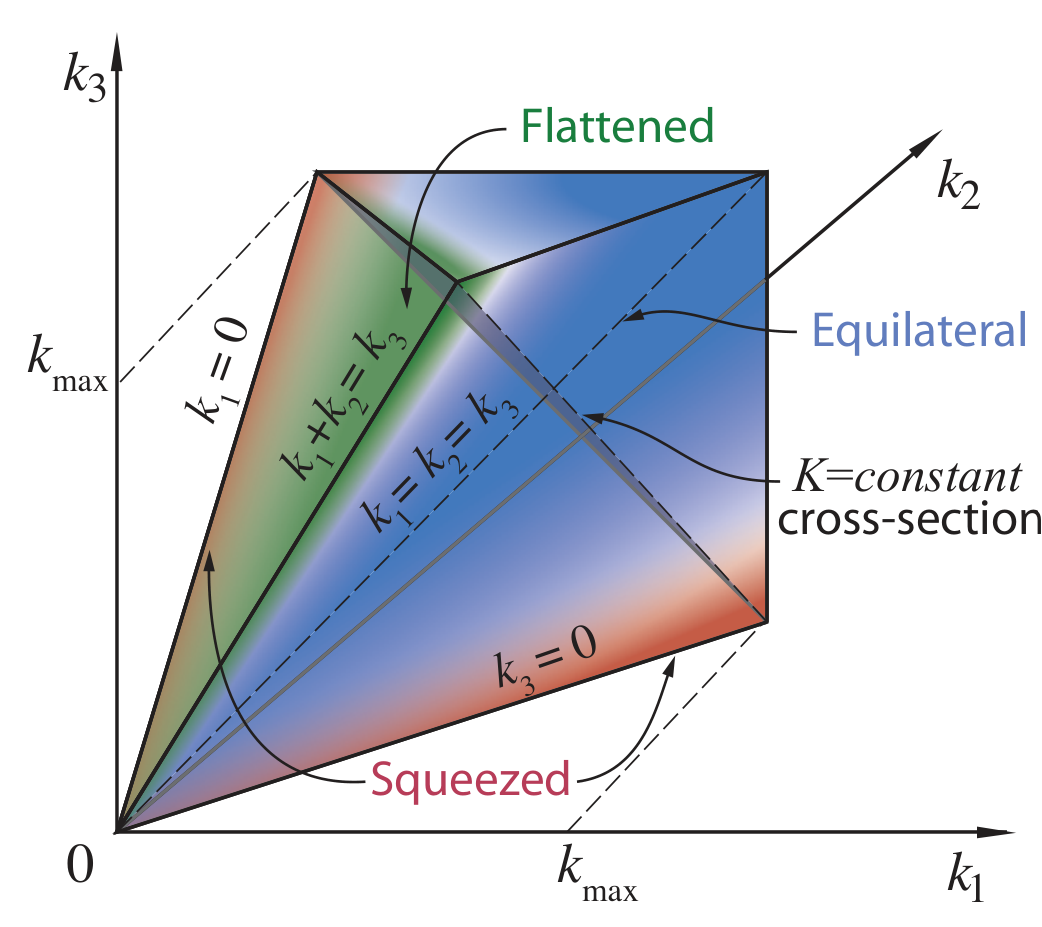
\includegraphics[width=\columnwidth]{plots/tetrapyd_3d_colour_split.png}}
\caption{
    Half of the tetrapydal region on which the bispectrum is defined,
    along with the various limits commonly discussed in the literature.
    We thank Paul Shellard for providing this figure.
}\label{fig:tetrapyd_diagram}
\end{figure}


The amplitude of a bispectrum shape is usually
quoted in terms of some amplitude parameter $\fnl^F$.
We can schematically define $\fnl^F$ for some template $F$ as follows:
\begin{equation}\label{def:fnl}
{
B^{F}(k_1,k_2,k_3) = \fnl^{F}\times F(k_1,k_2,k_3)
}
\end{equation}
where $F$ contains the dependence on the $k$-configuration.
This will be discussed further in later sections,
here we will merely note
%This definition coincides with the definitions of
%$\fnllocal$, $\fnlequil$ and $\fnlortho$
%when $F$ is (respectively) the local (see~\eqref{local_shape}),
%equilateral (see~\eqref{equil_shape}) and orthogonal templates,
%as defined in~\cite{Planck_NG_2013, Planck_NG_2015}.
that a distinction is sometimes made between the ``scale dependence''
of the bispectrum, meaning the dependence on $k_1+k_2+k_3$, and the ``shape dependence'',
meaning the dependence on each $k_i$ separately, for fixed $k_1+k_2+k_3$.


\section{Models}\label{sec:interactions}
We consider the same basic models as in~\cite{Funakoshi}.
Firstly, a quadratic potential
\begin{align}\label{eq:quadratic_potential}
    \quadpot = \frac{1}{2}m^2\phi^2
\end{align}
with a canonical kinetic term.
We will also consider a non-canonical model in detail, the $\dbi$ model.
    The $\dbi$ model has kinetic term
\begin{align}\label{eq:dbi_action}
    S_{\dbi}=\int d^4x\sqrt{-g}\left(-\frac{1}{f(\phi)}\left(\left(1+f(\phi)\partial_\mu\phi\partial^\mu\phi\right)^{\frac{1}{2}}-1\right)-V(\phi)\right),
\end{align}
and we choose
\begin{align}\label{eq:dbi_warp}
    f(\phi)=\frac{\lambda_{\dbi}}{\phi^4},\qquad
    V(\phi)=V_0-\frac{1}{2}m^2\phi^2,\qquad
    m=\sqrt{\beta_{IR}}H_{i}
\end{align}
where $\lambda_{\dbi}$, $\bir$ and $V_0$ are constants which
(along with the initial value of $\phi$, $\phi_0$) define the scenario in question.
$H_i$ is the Hubble parameter evaluated at the initial time.
This is in line with~\cite{Bean_ir_dbi, Chen_dbi}.


The energy-momentum tensor in~\eqref{einstein_equations}, in terms of the matter Lagrangian $\mathcal{L}_m$,
is given in~\eqref{gr_energy}.
%For a $P(X,\phi)$ model this evaluates to
%\begin{align}
%    T_{\mu\nu} &= g_{\mu\nu}P(X,\phi)+P_{,X}(X,\phi)\partial_{\mu}\phi\partial_{\nu}\phi\\
%            &\approx g_{\mu\nu}P(X,\phi)-2X\delta_{0\mu}\delta_{0\nu}P_{,X}(X,\phi).
%\end{align}
    Following~\cite{Christopherson_2009, mukhanov_1999},
    we can then use this to calculate the useful quantities
    \begin{align}
        P(X, \phi) &= -\frac{1}{f(\phi)}\left(\sqrt{1-2f(\phi)X}-1\right)-V(\phi)\\
        %P,_X(X, \phi) &= \frac{1}{\sqrt{1-2f(\phi)X}}\\
        %\rho(X, \phi) &= \frac{X}{\sqrt{1-f(\phi)X}}-P(X,\phi)\\
        %            &= \frac{1}{\sqrt{1-f(\phi)X}}(P+V)+V\\
        \rho(X, \phi) &= \frac{1}{f(\phi)}\left(\frac{1}{\sqrt{1-2f(\phi)X}}-1\right)+V(\phi)\\
        %\rho,_X(X, \phi) &= \frac{1}{\left(1-2f(\phi)X\right)^{\frac{3}{2}}}\\
        c^2_s(X, \phi) &= \frac{P,_X}{\rho,_X}\\
                    &= 1-2f(\phi)X
    \end{align}
    We see that, as expected, in the limit $\lambda_{\dbi}\rightarrow 0$, the sound
    speed tends to unity.
    From these quantities, we can calculate the $\phi$ equation of motion~\eqref{phieom}
    \begin{align}
        \phi'' &= -(3c_s^2-\varepsilon)\phi'
                -\frac{3f_\phi(\phi)}{2f(\phi)}\phi'^2
                +\frac{f_\phi(\phi)}{H^2f(\phi)^2}
                -\left(V_\phi(\phi)+\frac{f_\phi(\phi)}{f(\phi)^2}\right)\frac{c_s^3}{H^2}.
    \end{align}
    See~\cite{dbi_silverstein, warp_features_dbi} for further discussion,
    and also~\cite{cmb_pol_ics} for a brief discussion on setting consistent initial conditions.


\section{A field guide to $\fnl$}
    We present here some of the ways
    $\fnl$ is defined in the literature, for convenience.
    For the local form, one way of generating a non-Gaussian field
    is to write
    \begin{align}\label{fnllocal_quadratic}
        \zeta(\vecx) = \zeta_G(\vecx) - \frac{3}{5}\fnllocal\left(\zeta_G(\vecx)^2-\left<\zeta_G(\vecx)^2\right>\right)
    \end{align}
    where $\zeta_G(\vecx)$ is a Gaussian field. The parameter $\fnllocal$ therefore has a clear
    interpretation as parametrising the deviation from Gaussianity. From this form,
    one obtains a bispectrum of the form~\eqref{local_shape}. This is the version of $\fnl$
    that is most usually referred to.


    In~\cite{Planck_NG_2013}, $\fnl$ is defined individually for each template, in such a way
    that for some template $X$, in the equilateral limit $k_1=k_2=k_3$
    \begin{align}\label{planck_fnl_defn}
        B^X_\Phi(k,k,k) = \frac{6A_\Phi^2\fnl^X}{k^6},
    \end{align}
    for example equation $(5)$ in~\cite{Planck_NG_2013}.
    When considering a deviation from scale invariance, the form
    \begin{align}\label{planck_fnl_defn_ns}
        B^X_\Phi(k,k,k) = \frac{6A_\Phi^2\fnl^X}{k^{8-2n_s}},
    \end{align}
    is used,
    as in equation $(6)$ in~\cite{Planck_NG_2013}.
    The parameter $A_\Phi$ comes from
    \begin{align}
        P_\Phi(k) = \frac{A_\Phi}{k^{4-n_s}}\approx\left(\frac{3}{5}\right)^2\frac{H^2}{4\varepsilon c_sk^{4-n_s}}
    \end{align}
    where we used $\Phi=\frac{3}{5}\zeta$ and the slow-roll result for $P(k)$.
    In~\cite{seery_ng_0503, chen_ng_0605, dbi_in_the_sky} $\fnl$ is similarly defined in terms
    of the shape function evaluated on equilateral triangles,
    as the templates considered had no scale dependence.
    One particular example is the $\dbi$ template, which we will present explicitly in~\eqref{dbi_shape}.
    For now, we briefly state the definition of $\fnl^{\dbi}$, from~\cite{Planck_NG_2013}
    \begin{align}
        B^{\dbi}_\Phi(k,k,k) = \frac{6A_\Phi^2\fnl^{\dbi}}{k^{6}}.
    \end{align}
    Comparing to~\eqref{dbi_shape}, we find that
    \begin{align}\label{fnl_dbi_defn}
        \fnl^{\dbi} = -\frac{35}{108}\left(c_s^{-2}-1\right).
    \end{align}


    In~\cite{px_burrage, transport_main} we see $\fnl$ defined as the reduced bispectrum
    \begin{align}\label{transport_fnl_defn}
        \fnl(k_1,k_2,k_3) = \frac{5}{6}\frac{B(k_1,k_2,k_3)}{P(k_1)P(k_2)+P(k_1)P(k_3)+P(k_2)P(k_3)},
    \end{align}
    which depends on $k_1$, $k_2$ and $k_3$. In the local case we see that this reduces to
    the usual definition of $\fnllocal$ across the entire tetrapyd. %In the equilateral limit,
    %we see that it coincides with the definition of $\fnlequil$.


    In the template-free pipeline that we present in this work,
    we will take $\fnl$ as a fitting coefficient of our expansion
    of the numerically calculated primordial shape.
    This will be described in Chapter~\ref{chapter:constraints},
    where we will use an $\fnl$ which is scenario specific,
    and assessing the consistency of a scenario with data
    will be equivalent to assessing the consistency of $\fnl=1$.


    \subsection{Templates}
    The momentum dependence of the various possible bispectrum templates can be complex
    and it is therefore useful to define a standard notation in which to express this dependence.
    For example in~\cite{Fergusson_2010, Pajer_boostless_2020} the elementary
    symmetric polynomials are used to compactly represent the results in a way that is manifestly
    symmetric\footnote{This representation is useful here in presenting analytic templates, however in performing
    our calculations we will require a one-dimensional basis, not a basis in three variables.
    There are also numerical advantages to the Legendre polynomials, as discussed in~\cite{Fergusson_2010}.}.
    Here we will use the notation employed in~\cite{FergShell_2}:
\begin{align}\label{shape_notation}
\begin{split}
    K_p &= \sum_{i=1,2,3} k_i^p, \\
    K_{pq} &= \frac{1}{\Delta_{pq}}\sum_{i\neq j} k_i^p k_j^q,   \\
    K_{prs} &= \frac{1}{\Delta_{prs}}\sum_{i\neq j\neq l} k_i^p k_j^r k_l^s,
\end{split}
\end{align}
where $\Delta_{pq}$ is $2$ if $p=q$, $1$ otherwise
and $\Delta_{prs}$ is $6$ if $p=r=s$, $2$ if $p=r\neq s$ (and permutations),
and $1$ if $p,r,s$ are all distinct.


    The local template is the shape which results from assuming the perturbation is
    quadratic in a Gaussian field~\eqref{fnllocal_quadratic}
\begin{align}\label{local_shape}
S^{local}(k_1,k_2,k_3)
    &= \frac{6}{5}A_\zeta^2\fnllocal\left(\frac{k_1^2}{k_2k_3}+\frac{k_2^2}{k_3k_1}+\frac{k_3^2}{k_1k_2}\right)\\
    &= \frac{6}{5}A_\zeta^2\fnllocal\frac{K_3}{6\,K_{111}}.
\end{align}
This template peaks on squeezed triangles, i.e.\ when $k_1\approx k_2\gg k_3$,
and is used to test for multi-field effects~\cite{Planck_NG_2015}.
It can also be modified to include the expected scaling
\begin{align}
S^{local}(k_1,k_2,k_3)
    &= \frac{6}{5}\fnllocal\bigg(
        P_\zeta(k_2)P_\zeta(k_3)
        +P_\zeta(k_3)P_\zeta(k_1)
        +P_\zeta(k_1)P_\zeta(k_2)
    \bigg)(k_1k_2k_3)^2.
\end{align}


    Non-Gaussianity arising from inflation with a non-canonical kinetic term,
    and in the effective field theory of inflation~\cite{Cheung_eft, Baumann_horizon_2011},
    can typically be described by the equilateral template
\begin{align}\label{equil_shape}
    S^{equil}(k_1,k_2,k_3)
    &= \frac{18}{5}A_\zeta^2\fnlequil\frac{(k_2+k_3-k_1)(k_3+k_1-k_2)(k_1+k_2-k_3)}{k_1k_2k_3}
\end{align}
This template peaks on equilateral triangles, i.e.\ when $k_1\sim k_2\sim k_3$.


\subsection{Basic shapes}
    We will now briefly review the shape functions that result from
    standard canonical inflation, and from non-canonical $\dbi$ inflation.
    With a canonical kinetic term
    the slow-roll result for the shape is
\begin{align}\label{malda_shape}
    S^{Malda}(k_1,k_2,k_3) &= -\frac{1}{32}\frac{H^4}{12\varepsilon^2} \left( (3\varepsilon-2\eta)\frac{K_3}{K_{111}}+\varepsilon \left(K_{12}+8\frac{K_{22}}{K}\right) \right)
\end{align}
with $\eta=2\varepsilon$ for the quadratic potential~\eqref{eq:quadratic_potential}.
At the primordial level, this is well approximated by the separable local template~\eqref{local_shape}.
However, the amplitude of this shape is expected to be tiny,
since $S^{Malda}\sim\mathcal{O}(\varepsilon)\mathcal{P}^2_{\zeta}$
and the dominant contributions (the squeezed configurations) are expected
to have no observable effect~\cite{Cabass_2016}.


For the featureless $\dbi$ scenario, the shape function is~\cite{dbi_in_the_sky}:
\begin{align}\label{dbi_shape}
    %S^{DBI}(k_1,k_2,k_3) &= -\frac{1}{32}\frac{H^4}{12\varepsilon^2}\left(\frac{1}{c_s^2}-1\right)
    %     \frac{K_5+2K_{14}-3K_{23}+2K_{113}-8K_{122}}{K_{111}K^2}\\
    S^{\dbi}(k_1,k_2,k_3) &=\nonumber\\
    -\frac{35}{108}
         \left(\frac{1}{c_s^2}-1\right)&
         6\left(\frac{H^2}{4\varepsilon c_s}\right)^2
         \left(\frac{3}{5}\right)
         \left(-\frac{3}{7}\right)
         \frac{K_5+2K_{14}-3K_{23}+2K_{113}-8K_{122}}{K_{111}K^2}
\end{align}
to leading order in slow-roll.
Since the amplitude of this shape is predicted to be far larger than~\eqref{malda_shape}
($S^{\dbi}\sim\mathcal{O}(c_s^{-2})\mathcal{P}^2_{\zeta}$)
a constraint on the magnitude of this template can be translated into one 
on the effective sound speed. The \planck~analysis found a lower limit $c_s^{\dbi} \geq 0.087$
at $95\%$ significance~\cite{Planck_NG_2015}.
The shape~\eqref{dbi_shape} can be approximated by the separable equilateral template~\eqref{equil_shape}.


    \subsection{Scaling}
These templates can be modified to be more physically realistic by including
scaling similar to the scalar spectral index $n_s$~\cite{Planck_NG_2015}.
For example, we can add some scale dependence to the $\dbi$ template~\eqref{dbi_shape}
in a reasonable first approximation by including a prefactor,
as was done in~\cite{Planck_NG_2013}.
We define the product scaling template
\begin{align}\label{dbi_prod_shape}
    S^{\dbi}_{prod}(k_1,k_2,k_3) &= {\left(\frac{k_1k_2k_3}{k^3_\star}\right)}^{\frac{n_{NG}}{3}}S^{\dbi}(k_1,k_2,k_3)
\end{align}
and the sum scaling template
\begin{align}\label{dbi_sum_shape}
    S^{\dbi}_{sum}(k_1,k_2,k_3) &= {\left(\frac{k_1+k_2+k_3}{3k_\star}\right)}^{n_{NG}}S^{\dbi}(k_1,k_2,k_3)
\end{align}
with $n_{NG}=2(-2\varepsilon-\varepsilon_s-\eta)-2\varepsilon_s=2(n_s-1)-2\varepsilon_s$.
This improves the fit by matching the expected scaling of the shape function
along the equilateral limit, which results from slow-roll corrections.


\subsection{Shapes from features during inflation}
For our more stringent validation tests we work with feature model scenarios
based on the above base models.
It has long been known that sharp, localised features in the inflationary potential
can generate large non-Gaussianities~\cite{chen_easther_lim_1}, possibly with observable effects.
To explore non-Gaussianity coming from such sharp features we include
a kink~\cite{Adams_step}
\begin{align}\label{eq:kink_potential}
    V(\phi) = \quadpot\left(1-c\tanh\left(\frac{\phi_f-\phi}{d}\right)\right).
\end{align}
To explore non-Gaussianity from deeper in the horizon we imprint
extended resonant features on the basic potential
\begin{align}\label{eq:resonant_potential}
    V(\phi) = \quadpot\left(1+bf\sin\left(\frac{\phi}{f}\right)\right).
\end{align}
For more details on these models, see~\cite{chen_easther_lim_2}.


We now turn to feature templates that result from the preceding potential features.
The result of adding a feature of the form~\eqref{eq:kink_potential}
is to imprint oscillatory features on the bispectrum of the form
\begin{align}\label{cos_shape}
    S^{\cos}(k_1,k_2,k_3) \approx \cos(w(k_1+k_2+k_3))
\end{align}
though more realistically there is some phase, some shape dependence, and a modulating envelope,
as detailed in~\cite{adshead}.
The result of adding a resonant feature of the form~\eqref{eq:resonant_potential}
is to generate logarithmic oscillatory features in the shape function of the form
\begin{align}\label{ln_cos_shape}
    S^{\ln-\cos}(k_1,k_2,k_3) \approx \cos(w\ln(k_1+k_2+k_3)).
\end{align}
With a non-canonical kinetic term, this can also
cause oscillations in the folded limit (out-of-phase
with the equilateral oscillations) as well as a modulating shape,
as detailed in~\cite{chen_folded_resonant}.


    \section{Step 1: the interaction Hamiltonian}
    \subsection{Set-up}\
    %Since General Relativity has a diffeomorphism invariance, it has a redundancy
    %which must be settled before the true degrees of freedom are manifest.
    %One does this by decomposing the metric (typically in the $ADM$ formalism)
    %and expanding the action
    We begin with the action
    %S=\int dx^4\sqrt{g}\left[\frac{R}{2}-\frac{1}{2}(\nabla\phi)^2-V(\phi)\right].
    \begin{align}\label{gr_action}
        S=\int d^4x\sqrt{-g}\left[\frac{1}{2}R+P(X, \phi)\right].
    \end{align}
    Note that unlike~\eqref{inflaton_action} we have explicitly included the
    Ricci scalar $R$.
    One proceeds by expanding this action in the perturbations (typically
    using the ADM formalism)
    to obtain the constraint equations. One can then solve the constraints
    (perturbatively, aided by choice of gauge) and substitute
    back into the action, leaving only the dynamical variables.
    At the level of the background one then obtains the Friedmann equations;
    at second order one obtains the quadratic action, which evolves the
    free ``interaction picture'' fields, as we will discuss in Section~\ref{sec:in_in};
    and at third order, one obtains the cubic
    interaction Lagrangian, the source of deviations from Gaussianity.


    To write the Hamiltonian one needs the momentum $\pi$, conjugate to $\zeta$.
    For a simple Lagrangian such as $\mathcal{L}_{0}=\frac{1}{2}\dzeta^2$,
    we find $\pi\equiv\frac{\partial \mathcal{L}_0}{\partial \dzeta}=\dzeta$. However if the Lagrangian contains cubic terms
    containing $\dzeta$, this relation will change and may not be easily invertible.
    However one can show that it will still be true that $\mathcal{H}_{int}=-\mathcal{L}_{int}+\mathcal{O}(4)$,
    so calculating the cubic interaction Hamiltonian to third order in the perturbations
    from the cubic interaction Lagrangian is trivial\footnote{
        Ignoring terms with no time derivatives, take $\mathcal{L}=\frac{1}{2}\dzeta^2+g\dzeta^3$
        as an example.
        Then, $\pi=\frac{\partial\mathcal{L}}{\partial \dzeta}=\dzeta+3g\dzeta^2$.
        Calculating the Hamiltonian density
        \begin{align}
            \mathcal{H} &= \pi\dzeta - \mathcal{L}\\
                    &= \pi(\pi-3g\dzeta^2) - \frac{1}{2}(\pi-3g\dzeta^2)^2-g\dzeta^3\\
                    &\approx \frac{1}{2}\pi^2-3g\dzeta^3 +3g\dzeta^3-g\dzeta^3\\
                    &\approx \frac{1}{2}\pi^2-g\dzeta^3
        \end{align}
        where we have neglected terms higher order in the perturbations.
    }.


    We will work with a Hamiltonian that has been split into three parts,
    \begin{align}
        H = H_b + H_0 + \Hint,
    \end{align}
    where $H_b$ evolves the homogeneous background, $H_0$ is quadratic in $\zeta$ and evolves the free
    fields, and the interaction Hamiltonian $\Hint$ contains the terms cubic and above.
    In practice we will only use the part cubic in $\zeta$ and $\dzeta$,
    which can be labeled $\Hint^{(3)}$. We will use this to calculate
    the higher order correlations coming from the interactions. We will occasionally drop the superscript and
    refer to the cubic interaction Hamiltonian as simply the interaction Hamiltonian $\Hint$.


    \section{Step 2: the primordial bispectrum}\label{sec:inin_calc_example}
    \subsection{The in-in formalism}\label{sec:in_in}
The standard formalism for calculating
higher-order correlators for models of inflation is the in-in formalism~\cite{Maldacena,weinberg_in_in}.
For a careful discussion, see especially Appendix A2 of~\cite{weinberg_in_in}---here,
we will simply sketch the derivation.
See also~\cite{careful_contour},~\cite{Chen_review_2010, Babich_2004,
Renaux-Petel_2015, Meerburg_clock} for discussions and examples.
The setting for this calculation is the interaction picture. In the Schr\"{o}dinger
picture the time dependence is carried by the states, whereas in the Heisenberg picture
the time dependence is carried by the operators.
For notational convenience we will write the operator $\hat{H}$ as simply $H$.
We will also write $\tilH\equiv H_0+\Hint$ for the part of the Hamiltonian
which evolves the perturbations, which is order quadratic and higher,
since the linear part evolves the background fields.
We can write the solutions to the Schr\"{o}dinger and Heisenberg equations of motion
with reference to some initial time $t_i$, where we take the pictures to coincide:
\begin{align}
    \left|\psi,t\right>_S&=e^{-i\int_{t_i}^{t}{\tilH}dt}\left|\psi,t_i\right>_S\\
    \op_H(t) &= e^{i\int_{t_i}^{t}{\tilH}dt}\op_Se^{-i\int_{t_i}^{t}{\tilH}dt}
\end{align}
with $\op_S(t)=\op_S(t_i)$ and $\left|\psi,t\right>_H=\left|\psi,t_i\right>_S$.
We will be interested in the case where $\tau_i\rightarrow-\infty$.
In contrast to these two pictures,
the interaction picture splits the time dependence between the operators and
states---the operators evolve according
to the free Hamiltonian (the quadratic part) while the states see the interaction
\begin{align}
    \left|\psi,t\right>_I&=e^{i\int_{t_i}^{t}{\tilH}_0dt}e^{-i\int_{t_i}^{t}{\tilH}dt}\left|\psi,t_i\right>_S\\
    \op_I(t) &= e^{i\int_{t_i}^{t}{\tilH}_0dt}\op_Se^{-i\int_{t_i}^{t}{\tilH}_0dt}.
\end{align}


We wish to calculate the equal time expectation value of some operator $\left<\op(t)\right>$.
To calculate this directly is difficult for a theory with interactions.
In the interaction picture however, the operators evolve only according to the
free Hamiltonian, so their time dependence can be more easily obtained. To take advantage of this,
we would like to rewrite our desired expectation value as
\begin{align}
    \left<\op(t)\right> &= \left<F^{-1}(t,t_0)\op^I(t) F(t,t_0)\right>\label{heis_to_int}
\end{align}
to relate the correlators of the interacting theory to the correlators of the
free theory.
The operator $F$ is built out of two unitary time evolution operators
\begin{align}
    F(t,t_0) &= U_0^{-1}(t,t_0)U(t,t_0)\label{f_def}
\end{align}
that obey
\begin{align}
    U_0(t_0,t_0) = 1 = U(t_0,t_0).
\end{align}
As we will see, we will be able to roughly interpret $F(t,t_0)$ as evolving the interaction picture fields
back to the initial point $t_0$ (where the Heisenberg and interaction pictures coincide) and then
evolving the operators forward in the Heisenberg picture, giving the time evolution
of the full expectation value.


The operator $U(t,t_0)$ evolves the Heisenberg picture operators in time
using $\tilH$
\begin{align}
    \delphi(t) &= U^{-1}(t,t_0)\delphi(t_0)U(t,t_0)\\
    \delpi(t) &= U^{-1}(t,t_0)\delpi(t_0)U(t,t_0).
\end{align}
We can write the Heisenberg equation of motion, which has
explicit time dependence in $\tilH$ due to coefficients
that depend on the background evolution,
\begin{align}
    \frac{d}{dt}\delphi(\vecx,t) &= i\left[\tilH\left[\delphi(t),\delpi(t);t\right],\delphi\right].\label{heis_phi}
\end{align}
From this we can calculate
\begin{align}
    i\left[\tilH\left[\delphi(t),\delpi(t);t\right],\delphi\right]
    &= -U^{-1}\dot{U}U^{-1}\delphi(t_0) U+U^{-1}\delphi(t_0) \dot{U}\\
    &= -U^{-1}\dot{U}\delphi(t)+\delphi(t)U^{-1} \dot{U}\\
    &= \left[-U^{-1}\dot{U},\delphi(t)\right]
\end{align}
where $\dot{U}=\frac{dU}{dt}$,
and we have temporarily omitted the arguments of $U(t,t_0)$.
We then have
\begin{align}
    \frac{d}{dt}U(t,t_0) &= -iU(t,t_0)\tilH\left[\delphi(t),\delpi(t);t\right]U^{-1}(t,t_0)U(t,t_0)\\
    \implies \frac{d}{dt}U(t,t_0) &= -i\tilH\left[\delphi(t_0),\delpi(t_0);t\right]U(t,t_0)\label{u_def}
\end{align}
where particular attention should be paid to the evaluation time of the operators from
which the $\tilH$ is built.


In contrast, $U_0(t,t_0)$ evolves the interaction picture operators in time
using only the part of the Hamiltonian quadratic in the perturbations
\begin{align}
    \delphi^I(t) &= U_0^{-1}(t,t_0)\delphi^I(t_0)U_0(t,t_0)\\
    \delpi^I(t) &= U_0^{-1}(t,t_0)\delpi^I(t_0)U_0(t,t_0)
\end{align}
which by a similar calculation (recalling that $\delphi^I$ evolves
according to the Heisenberg equation of motion with $H_0$) gives us
\begin{align}
    \frac{d}{dt}U_0(t,t_0) &= -iH_0\left[\delphi^I(t_0),\delpi^I(t_0);t\right]U_0(t,t_0).\label{u0_def}
\end{align}


From~\eqref{f_def},~\eqref{u_def} and~\eqref{u0_def} we can find the equation of motion for $F(t,t_0)$
\begin{align}
    \frac{d}{dt}F(t,t_0) &= -i\Hint\left[\delphi^I(t),\delpi^I(t);t\right]F(t,t_0)
\end{align}
where $\Hint$ is cubic and higher order in the perturbations,
but is now built from the interaction picture fields evaluated at $t$.
This can be solved using the standard time ordering operator $T$
\begin{align}\label{f_soln}
    F(t,t_0) = T\exp\left(-i\int^t_{t_0}\Hint(t)dt\right).
\end{align}


We have not yet accounted for the evolution of the vacuum state.
We wish the interacting vacuum $\left|\Omega\right>$
to coincide with the free vacuum $\left|0\right>$ in the far past.
We achieve this by taking the integration contour in~\eqref{f_soln} to be
moved slightly onto the complex plane, introducing a factor which kills off the
interactions in the distant past~\cite{Maldacena}.
That is, instead of taking
$\tau_0=-\infty$ we take $\tau_0=-\infty(1+i\epsilon)$.
This is known as the $i\epsilon$ prescription.
To calculate $F^{-1}$, we must take care to use the anti-time ordering operator,
and take the lower bound of the integration to be $-\infty(1-i\epsilon)$.


We would like to calculate the bispectrum of $\zeta$ at tree level.
Expanding~\eqref{f_soln} in~\eqref{heis_to_int}, and recalling that
the expectation value of a product of three interaction picture fields vanishes
\begin{align}\label{inin_integral}
{
    \left< \zeta_{\mathbf{k_1}}(\tau)\zeta_{\mathbf{k_2}}(\tau)\zeta_{\mathbf{k_3}}(\tau) \right>
=-i\int_{-\infty(1-i\varepsilon)}^{\tau}d\tau'a(\tau')
    \left<0\lvert \zeta_{\mathbf{k_1}}(\tau)\zeta_{\mathbf{k_2}}(\tau)\zeta_{\mathbf{k_3}}(\tau)\Hint(\tau') \rvert0\right>+c.c
}
\end{align}
where all the operators on the right-hand side are in the interaction picture
and $\Hint$ is the interaction Hamiltonian written in terms of $\zeta$ and its
(interaction picture) conjugate momentum $\dzeta$.
We will now take $\Hint$ to contain only terms cubic in the perturbations.
From this calculation we obtain the dimensionless shape function $S(k_1,k_2,k_2)$,
defined in~\eqref{shapefn},
which is then used as input into~\eqref{eq:reduced_cmb}.
As an example, if one takes $\Hint\propto\dot{\zeta}^3$, this set-up can produce the standard EFT shape
\begin{align}\label{example_eft2}
    S(k_1, k_2, k_3) = \frac{k_1k_2k_3}{(k_1+k_2+k_3)^3}.
\end{align}

The central point, as noticed in~\cite{Funakoshi}, is that the
integrand of~\eqref{inin_integral} is intrinsically separable
in its dependence on $k_1$, $k_2$ and $k_3$, and that the time integral
can be done in such a way as to preserve this separability.
This intrinsic separability has clearly been lost in
the example in~\eqref{example_eft2},
but can be regained (to arbitrary numerical precision) by approximating it
with a sum of separable terms. Our general aim will be to directly calculate
this sum for a broad range of inflation models.


%We now briefly outline the set-up of the standard calculation.
%The Lagrangian is expanded in the perturbations and used to obtain the Hamiltonian.
%The Hamiltonian for the perturbations is split into $H_0$ and $\Hint$.
%The first part is used to evolve the interaction picture fields, $\zeta_I$,
%which we will simply refer to as $\zeta$, as in~\eqref{inin_integral}.
%The perturbations see an interaction Hamiltonian $\Hint$,
%of which we will consider the part cubic in the perturbations,
%with time dependent coefficients due to the evolution of the background fields.
%The perturbations are assumed to be initially in the Bunch-Davies vacuum,
%but the non-linear
%evolution introduces correlations between the modes.
%As the modes cross the horizon they begin to behave classically
%and eventually freeze out.


There is some freedom in how to represent the interaction Hamiltonian,
as the equation of motion of the free fields can be used, along with integration by parts~\cite{rp_integ_by_parts}.
This can be used, as pointed out in~\cite{Funakoshi}, to avoid numerically difficult cancellations.
Some presentations of this calculation use a field redefinition to eliminate terms
proportional to the equation of motion from the Lagrangian.
As pointed out in~\cite{px_burrage},
this is unnecessary as these terms will never contribute to the bispectrum result.
In fact, in some scenarios (such as resonant models) it introduces a numerically difficult
late time cancellation between a term in the interaction Hamiltonian and the
correction to the correlator that adjusts for the field redefinition.


%The bispectrum arising from a single field inflation model,
%with a canonical kinetic term, slowly rolling, turns out to produce
%unobservably small non-Gaussianity~\cite{Maldacena}.
%However, by breaking these assumptions large signals can arise.
%These signals are usually calculated using~\eqref{inin_integral} within tailored approximations.
%The results are not always separable, so further approximations must then be made to
%allow comparison with the CMB.


We now detail an explicit example of an in-in calculation.
We will take
\begin{align}\label{hint_example}
    \Hint=\int d^3x~g(t) a^3{\dzeta^3}
\end{align}
where $g(t)$ is some function of time.
This example is particularly simple as it contains no spatial derivatives.
We will include those when we outline our formalism fully in Section~\ref{sec:setting_notation}.
We wish to calculate
\begin{align}\label{inin_example}
    \left<\zeta_{\mathbf{k_1}}(t)\zeta_{\mathbf{k_2}}(t)\zeta_{\mathbf{k_3}}(t)\right>&=
    \Re\left(\left<-2i \zeta^I_{\mathbf{k_1}}(t)\zeta^I_{\mathbf{k_2}}(t)\zeta^I_{\mathbf{k_3}}(t)
    \int_{-\infty(1+i\varepsilon)}^{t}dt'\Hint(t')
    \right>\right).
\end{align}
We note that the operators inside the expectation value on the right hand side are
time-ordered, as $t'\leq t$.
All the operators on the right hand side are in the interaction picture, though for
notational convenience we will drop the superscript $I$.
To proceed with this calculation we will use Wick's theorem
\begin{align}\label{wick}
    \left<0\left|\zeta_{\mathbf{k_1}}\ldots\zeta_{\mathbf{k_n}}\right|0\right>
    &= \left<0\left|:\zeta_{\mathbf{k_1}}\ldots\zeta_{\mathbf{k_n}}:~+:\sum~\text{pairwise contractions:}~\right|0\right>
\end{align}
where $:~:$ denotes normal ordering. Normal ordering places operators so that those
which annihilate $\left|0\right>$ are to the right and those which annihilate
$\left<0\right|$ are put to the left. Thus, if a normal ordered term contains
uncontracted operators, the term vanishes inside an expectation value.


By ``$\sum$ pairwise contractions'' we mean the sum over every possible permutation of contracting one pair,
and of contracting two pairs, and so on.
The contraction of two operators $\zeta_{\mathbf{k_1}}$ and $\zeta_{\mathbf{k_2}}$
is defined as the difference between their time ordered product and their normal ordered product.
Since the operators are built up of creation and annihilation operators, this will simply
vanish, or
be proportional to the commutator of $\hat{a}$ and $\hat{a}^{\dagger}$.
In either case, it can be pulled out of the expectation value.
Therefore, the only surviving contribution will the term with every $\zeta_{\mathbf{k}}$
contracted in a pair.


To evaluate the pairwise contractions we expand $\zeta$ similarly to~\eqref{operator_expansion},
\begin{align}
    \left<\zeta_{\mathbf{k_1}}(t_1)\zeta_{\mathbf{k_2}}(t_2)\right>
    &= \left<0\left|
            \left(\zeta_{k_1}(t_1)\hat{a}_\mathbf{k_1} +
            \zeta^*_{k_1}(t_1)\hat{a}^{\dagger}_{-\mathbf{k_1}}\right)
            \left(\zeta_{k_2}(t_2)\hat{a}_\mathbf{k_2} +
            \zeta^*_{k_2}(t_2)\hat{a}^{\dagger}_{-\mathbf{k_2}}\right)
        \right|0\right>\\
    &= \left<0\left|
            \zeta_{k_1}(t_1)\hat{a}_\mathbf{k_1}
            \zeta^*_{k_2}(t_2)\hat{a}^{\dagger}_{-\mathbf{k_2}}
        \right|0\right>\\
    &= \zeta_{k_1}(t_1)\zeta^*_{k_2}(t_2)\left<0\left|
            \left[\hat{a}_\mathbf{k_1},
            \hat{a}^{\dagger}_{-\mathbf{k_2}}\right]
        \right|0\right>\\
    &= \zeta_{k_1}(t_1)\zeta^*_{k_2}(t_2)(2\pi)^3\delta^{(3)}(\mathbf{k_1}+\mathbf{k_2})
\end{align}
where we used~\eqref{creation_annihilation_commutator}.


Inserting~\eqref{hint_example} into~\eqref{inin_example}
%and rewriting $\dzeta(\vecx)$ in terms of its Fourier transform,
we get
\begin{align}\label{inin_example_start}
    \left<\zeta_{\mathbf{k_1}}(t)\right.&\left.\zeta_{\mathbf{k_2}}(t)\zeta_{\mathbf{k_3}}(t)\right>\\
    &=\Re\left(\left<-2i \zeta_{\mathbf{k_1}}(t)\zeta_{\mathbf{k_2}}(t)\zeta_{\mathbf{k_3}}(t)
    \int_{-\infty(1+i\varepsilon)}^{t}dt'
    \int d^3x~\left(g(t) a^3\dzeta^3(\vecx,t')\right)
    \right>\right).
\end{align}
Continuing, we replace $\zeta$ with its Fourier transform
\begin{align}\label{inin_example_2}
    \bigg<-2i \zeta_{\mathbf{k_1}}(t)&\zeta_{\mathbf{k_2}}(t)\zeta_{\mathbf{k_3}}(t)
    \int_{-\infty(1+i\varepsilon)}^{t}dt'
    \int d^3x~\left(g(t) a^3\dzeta^3(\vecx,t')\right)
    \bigg>\\
    =&\bigg<-2i \zeta_{\mathbf{k_1}}(t)\zeta_{\mathbf{k_2}}(t)\zeta_{\mathbf{k_3}}(t)
    \int_{-\infty(1+i\varepsilon)}^{t}dt'\left(g(t) a^3\right)\nonumber\\
    &\qquad\cdot
    \int \frac{d^3p}{(2\pi)^3}
    \frac{d^3q}{(2\pi)^3}
    \frac{d^3r}{(2\pi)^3}
    \dzeta_{\mathbf{p}}(t')
    \dzeta_{\mathbf{q}}(t')
    \dzeta_{\mathbf{r}}(t')
    \int d^3x e^{i\vecx\cdot(\mathbf{p}+\mathbf{q}+\mathbf{r})}
    \bigg>\\
    =&\bigg<-2i \zeta_{\mathbf{k_1}}(t)\zeta_{\mathbf{k_2}}(t)\zeta_{\mathbf{k_3}}(t)
    \int_{-\infty(1+i\varepsilon)}^{t}dt'\left(g(t) a^3\right)\nonumber\\
    &\qquad\cdot
    \int \frac{d^3p}{(2\pi)^3}
    \frac{d^3q}{(2\pi)^3}
    \frac{d^3r}{(2\pi)^3}
    \dzeta_{\mathbf{p}}(t')
    \dzeta_{\mathbf{q}}(t')
    \dzeta_{\mathbf{r}}(t')
    (2\pi)^3\delta^{(3)}(\mathbf{p}+\mathbf{q}+\mathbf{r})
    \bigg>.
\end{align}
We now perform the contractions. If we contract one of the $\zeta_{\mathbf{k_i}}$ with
another, then the delta function will force one of $\mathbf{p}$, $\mathbf{q}$
or $\mathbf{r}$ to be zero. Since we want $\zeta_\mathbf{k}$ to be a perturbation
and not a contribution to the background, this cannot contribute.

The results of the contractions will therefore have the form
\begin{align}
    \left<\zeta_{\mathbf{k_1}}(t)\dzeta_{\mathbf{p}}(t')\right>
    &= \zeta_{k_1}(t)\dzeta^*_{p}(t')(2\pi)^3\delta^{(3)}(\mathbf{k_1}+\mathbf{p}).
\end{align}
and permutations.
Using the delta functions to perform the momentum integrals,
switching to conformal time,
and recalling~\eqref{bispectrum_definition}, we obtain
\begin{align}\label{inin_computer}
    B(k_1, k_1,&k_3)
    =
    \Re\bigg(-2i \zeta_{k_1}(0)\zeta_{k_2}(0)\zeta_{k_3}(0)\nonumber\\
    &\cdot\int_{-\infty(1+i\varepsilon)}^{0}d\tau'\bigg(g(\tau') a^4(\tau')\bigg)
    \dzeta^*_{k_1}(\tau')
    \dzeta^*_{k_2}(\tau')
    \dzeta^*_{k_3}(\tau')
    +\text{perms}
    \bigg).
\end{align}
If one wanted to numerically calculate the bispectrum resulting from~\eqref{hint_example},
one could use this form. Until this point we have assumed nothing about the solutions of the
equations of motion, and we have not made a slow-roll approximation (although we have
of course only included the tree-level effects).
After one had chosen some prescription for numerically implementing the
$i\varepsilon$ prescription, one would need to evolve a set of $\zeta_{k}$
according to the equations of motion and then perform the above time integral.


This is the point where our work will diverge from the standard calculation---this
will be detailed in Section~\ref{sec:setting_notation}. For now, we merely note that
the integrand of~\eqref{inin_computer} is explicitly separable in $k_1$, $k_2$ and $k_3$.


We will now continue the calculation within the slow-roll approximation,
using~\eqref{uk_solution}. We approximate $g(\tau')$ and the slow-roll
parameters as constant, and use $a\approx-1/(H\tau)$.
We see that we will need to perform the following integral by parts
\begin{align}
    \int_{-\infty(1+i\varepsilon)}^{0}d\tau~\tau^2 e^{-ic_sK\tau}
    &= \frac{-2i}{c_s^3K^3}
\end{align}
where we recall $K=k_1+k_2+k_3$.
Using this, we finally obtain
\begin{align}
    S(k_1, k_2, k_3) = -3\frac{g H^5}{8\varepsilon^3}\frac{k_1k_2k_3}{(k_1+k_2+k_3)^3}
\end{align}
where the factor of $6$ comes from the different possible contractions, all
of which give the same result in this example.
We can make contact with $\fnl^{EFT2}$ of~\cite{Planck_NG_2018, Senatore_wmap_2009}
by setting $g(t)=-\frac{\varepsilon}{Hc_s^2}(1-c_s^2)\left(1+\frac{2\tilde{c}_3}{3c_s^2}\right)$
and recalling $\Phi=\frac{3}{5}\zeta$.


    \subsection{The squeezed limit consistency condition}
The squeezed limit of single-field bispectra will not cause
observable deviations from a Gaussian universe,
due to a cancellation when switching to physical coordinates~\cite{Cabass_2016}.
Here, we will only consider primordial phenomenology
in comoving coordinates, so despite this cancellation,
the squeezed limit is still a useful validation test of our results,
using the standard single-field squeezed limit consistency condition~\cite{sqz_consistency,not_so_sqz}.
With $\mathbf{k_S}\equiv\left(\mathbf{k_2}-\mathbf{k_3}\right)/2 $:
\begin{align}\label{eq:sqz_consistency}
    S(k_1,k_2,k_3) = -\left[(n_s-1)|_{k_S}+\mathcal{O}\left(\frac{k_1^2}{k_S^2}\right)\right]P_{\zeta}(k_1)P_{\zeta}(k_S),
\ \ \  k_1\ll k_S
\end{align}
where $S(k_1,k_2,k_3)$ is again our dimensionless shape function.
That the error in the consistency relation decreases at least quadratically
in the long mode was shown in~\cite{not_so_sqz}.
We will use~\eqref{eq:sqz_consistency} in Chapter~\ref{chapter:methods}
as a check on our results.


\section{Step 3: the $\cmb$ bispectrum}
    %For a three dimensional statistical distribution projected onto
    %a sphere, we expect the three-point statistics to be projected
    %like
    %\begin{align}
    %    \left<f_{l_1m_1}f_{l_2m_2}f_{l_3m_3}\right> = B_{l_1l_2l_3}{{l_1~~l_2~~l_3} \choose {m_1~m_2~m_3}}
    %\end{align}
    %where ${{l_1~~l_2~~l_3} \choose {m_1~m_2~m_3}}$ enforces statistical isotropy.
    In this section we will present a basic example of how the primordial bispectrum
    $B(k_1, k_2, k_3)$ is connected to the $\cmb$ bispectrum, which will be discussed in more
    detail in the next section.
    For the $\cmb$, we calculate the reduced $\cmb$ bispectrum using~\cite{FergShell_2}
    \begin{equation}
    \label{eq:reduced_cmb}
    b_{l_1l_2l_3} = \left(\frac{2}{\pi}\right)^3\int_{0}^{\infty}dr~r^2
        \int d^3k~(k_1k_2k_3)^2 B_{\Phi}(k_1,k_2,k_3)\prod_{i=1}^{3}\left[j_{l_i}(k_ir)\Delta_{l_i}(k_i)\right],
    \end{equation}
    analogously to~\eqref{eqn:transfer_function}.
    We see that the expression for the shape function $(k_1k_2k_3)^2 B_{\Phi}(k_1,k_2,k_3)$ appears directly.


    We will repeat the simple example outlined in~\cite{FergShell_2}. If we
    take ${S(k_1,k_2,k_3)=1}$ for all configurations, then the above four-dimensional integral
    simplifies greatly. If we also restrict to large angular scales
    % (The first acoustic peak is around l=200.)
    then we can use the same large-scale Sachs-Wolfe approximation\footnote{
    The factor of $3$ in this equation compared to the factor of $5$
    in~\eqref{sachs_cl_example} is due to $\zeta=5\Phi/3$
    on large scales during matter domination.
    % See (3.47) of AC.
}
    that was used in Section~\ref{sec:power_spec_estimator}
    \begin{align}
        \Delta_l(k) = \frac{1}{3}j_l(\chi_*k)
    \end{align}
    where $\chi_*$ is the comoving distance to last scattering.
    The integral then becomes
    \begin{equation}
    \label{eq:reduced_cmb_constant}
    b_{l_1l_2l_3} = \left(\frac{2}{3\pi}\right)^3\int_{0}^{\infty}drr^2
        \int d^3k \prod_{i=1}^{3}\left[j_{l_i}(k_ir)j_l(\chi_*k_i)\right].
    \end{equation}
    Using the following result
    \begin{align}
        \int_0^\infty dk~j_l(k)j_l(xk)\qquad=\qquad&\frac{\pi}{2}\frac{x^{-(l+1)}}{2l+1}\qquad&&\text{for $x>1$}\\
                            =\qquad&\frac{\pi}{2}\frac{x^{l}}{2l+1}\qquad&&\text{for $x<1$}
    \end{align}
    we arrive at an expression for the $\cmb$ angular bispectrum
    \begin{align} 
        b_{l_1l_2l_3} &= \frac{f_{NL}}{27}\frac{1}{(2l_1+1)(2l_2+1)(2l_3+1)}
        \left[\int^1_0dx x^{l_1+l_2+l_3+2}+\int^\infty_1dx x^{-l_1-l_2-l_3-1}\right]\label{eq:bll_constant_integral}\\
                &= \frac{f_{NL}}{27}\frac{1}{(2l_1+1)(2l_2+1)(2l_3+1)}
        \left[\frac{1}{l_1+l_2+l_3+3}+\frac{1}{l_1+l_2+l_3}\right]\label{eq:bll_constant}.
    \end{align}
    Note also that the acoustic oscillations and
    other relevant physics have not been taken
    into account here---these would imprint oscillations at higher $l$.
    Nevertheless, it is instructive to write down the scaling behaviour of this
    simple example, and to see how separability is lost between~\eqref{eq:reduced_cmb_constant}
    and~\eqref{eq:bll_constant} even for this simple case.


    \section{Step 4: $\cmb$ bispectrum estimation}
    \subsection{Linear regression}
    % https://arxiv.org/pdf/1006.1642.pdf
    % https://arxiv.org/pdf/0912.5516.pdf
    The $\cmb$ bispectrum derived from a given inflationary scenario is denoted
    \begin{align}
        %\left<\triplea\right> = B^{l_1l_2l_3}_{m_1m_2m_3} = \mathcal{G}^{l_1l_2l_3}_{m_1m_2m_3}b_{l_1l_2l_3}.
        \left<\triplea\right> = \mathcal{G}^{l_1l_2l_3}_{m_1m_2m_3}b_{l_1l_2l_3}
    \end{align}
    where isotropy demands that $b_{l_1l_2l_3}$ does not depend on the $m_i$,
    and the quantity $\mathcal{G}^{l_1l_2l_3}_{m_1m_2m_3}$ is the Gaunt integral
    \begin{align}
        \mathcal{G}^{l_1l_2l_3}_{m_1m_2m_3} &\equiv \int d\Omega Y_{l_1m_1}\nhatbrkt Y_{l_2m_2}\nhatbrkt Y_{l_3m_3}\nhatbrkt. %\\
        %&= \sqrt{\frac{(2l_1+1)(2l_2+1)(2l_3+1)}{4\pi}}
        %{{l_1~~l_2~~l_3} \choose {0~~0~~0}}{{l_1~~l_2~~l_3} \choose {m_1~m_2~m_3}}\\
        %&= h_{l_1l_2l_3}{{l_1~~l_2~~l_3} \choose {m_1~m_2~m_3}}
    \end{align}
    %where we have used the Wigner $3j$ symbol, and defined $h_{l_1l_2l_3}$.
    The bispectrum measured from the $\cmb$ is denoted
    \begin{align}
        %B^{obs,l_1l_2l_3}_{m_1m_2m_3} &= \tripleaobs.
        \mathcal{G}^{l_1l_2l_3}_{m_1m_2m_3}b^{obs}_{l_1l_2l_3} &= \tripleaobs.
    \end{align}
    %We can write the angle averaged bispectrum
    %\begin{align}\label{eq:bll}
    %    B_{l_1l_2l_3} = \sum_{m_i} {{l_1~~l_2~~l_3} \choose {m_1~m_2~m_3}} B^{l_1l_2l_3}_{m_1m_2m_3}.
    %\end{align}


    The standard method for estimating the $\cmb$ bispectrum is to calculate the least squares
    fit between the theory bispectrum and the observed bispectrum. That is, we find $\lambda$
    such that the following expression is minimised:
    \begin{align}
        L=\sum_{l_i,m_i}{\left(\lambda\frac{\left<\triplea\right>}{\sqrt{C_{l_1}C_{l_2}C_{l_3}}}
                - \frac{\tripleaobs}{\sqrt{C_{l_1}C_{l_2}C_{l_3}}}\right)}^2.
    \end{align}
    The solution to this is simply
    \begin{align}
        \lambda = \frac{\frac{\left<\triplea\right>}{\sqrt{C_{l_1}C_{l_2}C_{l_3}}}\cdot\frac{\tripleaobs}{\sqrt{C_{l_1}C_{l_2}C_{l_3}}}}{\left|\frac{\left<\triplea\right>}{\sqrt{C_{l_1}C_{l_2}C_{l_3}}}\right|^2}
    \end{align}
    where $\cdot$ denotes summation over $l_i$ and $m_i$.
    Defining the normalisation~\cite{Fergusson_polyspectra, Fergusson_efficient} 
    \begin{align}
        N_B = \sum_{l_i,m_i}\frac{\left(\mathcal{G}^{l_1l_2l_3}_{m_1m_2m_3}b_{l_1l_2l_3}\right)^2}{C_{l_1}C_{l_2}C_{l_3}}
    \end{align}
    we can rewrite this in the usual way (with $\lambda$ identified as the result of the estimator, $\epsilon$)
    \begin{align}
        \epsilon = \frac{1}{N_B}\sum_{l_i,m_i}\frac{\left<\triplea\right>\tripleaobs}{C_{l_1}C_{l_2}C_{l_3}}.
    \end{align}
    This estimator is optimal~\cite{Babich:2005en}, so its variance
    saturates the Cramer-Rao bound and can be calculated theoretically.
    %However, if we simply calculate this quantity for some theoretical model we will not be able to
    %interpret the result. This is because even a $\cmb$ sky in a universe with initial conditions
    %drawn from a purely Gaussian distribution will, through random chance,
    %result in a non-zero $\epsilon$. This problem is solved using simulated Gaussian maps. 


    This procedure must be modified to account for experimental noise, beam effects and
    the presence of a mask (to exclude to regions of the sky saturated by our galaxy
    and other foreground contaminants).
    The covariance matrix is approximated as diagonal, and the
    following quantities are defined
    \begin{align}
        %C_{l_1m_1,l_2m_2}&\approx C_l\delta_{l_1l_2}\delta_{m_1~-m_2},\label{diagonal_covariance}\\
           \tilde{C_l} &\equiv b_l^2C_l+N_l,\\
           \tilde{b}_{l_1l_2l_3} &\equiv b_{l_1}b_{l_2}b_{l_3}b_{l_1l_2l_3},
    \end{align}
    to incorporate the experimental beam $b_l$ and the noise power
    spectrum $N_l$ from the experiment.
    The estimator can then be written as~\cite{Creminelli:2005hu, Fergusson_polyspectra, Fergusson_efficient}
    \begin{align}\label{estimator_with_linear}
        \epsilon = \frac{1}{N_B^2}\sum_{l_im_i}
        \frac{\mathcal{G}^{l_1l_2l_3}_{m_1m_2m_3}\bar{b}_{l_1l_2l_3}}{\tilde{C}_{l_1}\tilde{C}_{l_2}\tilde{C}_{l_3}}
        \left(\triplea-3C^{sim}_{l_1m_1,l_2m_2}a_{l_3m_3}\right)
    \end{align}
    which retains optimality~\cite{Creminelli:2005hu}.
    Here, the diagonal approximation is insufficient for the linear term
    (which is especially important for local type shapes), so the
    full covariance matrix $C^{sim}_{l_1m_1,l_2m_2}$ is approximated using an ensemble average
    over a suite of Gaussian simulations. Excluding this term would result in a large false
    detection of non-Gaussianity, due to the effects of masking the part of the sky obscured
    by the galaxy. While the estimator is still optimal,
    Monte Carlo simulations are also used to estimate the variance, to ensure systematics
    are taken into account correctly.
    Many $\cmb$ skies are generated from Gaussian initial conditions, and then the estimator
    is applied to each. This gives a distribution of $\epsilon$, from which we can
    calculate $1\sigma$ and $2\sigma$ regions for $\epsilon$. Then the result of the
    estimator (when applied to the real $\cmb$ sky) can be compared to this distribution
    to determine the significance of the result.



    \subsection{Complexity of bispectrum estimation}
    %The bispectrum, like the power spectrum, is a quantity that describes
%the statistical distribution of which our universe is a single realisation.
%We can use this one accessible sky to constrain inflationary physics; 
%see~\cite{astro2020_png, astro2020_features, Ballardini_2017, Sypsas_2017,
%    Palma_2017} for recent reviews.
%There are two parts to the pipeline of bispectrum estimation.
%Firstly, calculating the primordial bispectrum at the end of some inflation scenario,
%and then calculating the effect this bispectrum
%has on some appropriate observable today.
To calculate the bispectrum of temperature fluctuations in the CMB, 
one uses transfer functions
(which we saw previously in~\eqref{eqn:transfer_function})
to evolve and project the primordial bispectrum onto our sky.
In principle, this is the same process as power spectrum estimation.
However, for the bispectrum the computational challenge is far greater,
requiring both compute-intensive and large in-memory components.
As a result of this complexity, this step is computationally impractical for generic primordial bispectra.
Progress can be made by finding an approximation to the primordial shape
that is separable, and using this simplification
to make the calculation tractable
through the $\ksw$ estimator~\cite{Komatsu_2005, Munchmeyer_2014, Smith_2011}.
For example, one may find that a particular inflation scenario generates
a primordial bispectrum with a high correlation with some standard shape,
then look at how well that standard shape is constrained by the CMB.
The Modal decomposition method of~\cite{FergShell_1,FergShell_2,FergShell_3}
leveraged these simplifications in a more structured way
for generic bispectra, broadening the range of constrained models.


The measure of non-Gaussianity in the CMB that is
most usually quoted is $\fnl$, referring to $\fnllocal$.
This number describes how well a particular template, the local template,
describes the correlations in the CMB;
this template is used as a proxy for the class of inflation models that produce similar bispectra.
Similar quantities for the equilateral and orthogonal templates are also
commonly quoted.
In addition to broadening the range of constrained models through increases in efficiency,
the Modal decomposition method of~\cite{FergShell_1,FergShell_2,FergShell_3}
allows to go beyond this paradigm, efficiently constraining inflationary templates in the CMB using
all of the shape information; essentially constraining an $\fnl$
specific to a given template. This bypasses the approximation step at the level of the templates,
of finding a separable approximation to the primordial template.
The results of these methods are constraints on the parameters of
certain inflation models through the approximate phenomenological templates.
These constraints can be found in~\cite{Planck_NG_2015, Planck_NG_2018}.


The numbers $\fnl^F$ are useful summary parameters.
From the data-side, they represent the result of
a complex and intensive process
of estimating the amplitude of the template $F$,
given some data. From the theory-side, one
can use them to take an inflation scenario and compare it
to that data, if one can find a standard template
with a high correlation with the shape resulting
from that scenario.
However, despite its usefulness, this paradigm does
have drawbacks. It acts as an information bottleneck,
losing some constraining power when one approximates
the real shape function by some standard template.
In particular, if one is interested in a feature model,
it may be be difficult to see how constraints on existing
features can be applied.


Recall the definition of separability~\eqref{sepXYZ}.
The link between the separability of the primordial bispectrum
and the reduced CMB bispectrum can be seen from~\eqref{eq:reduced_cmb}.
If the primordial bispectrum is separable then the overall dimension
of the calculation can be reduced from seven to five in~\eqref{eq:reduced_cmb},
since the spherical Bessel functions $j_{l_i}$ and the
transfer functions $\Delta_{l_i}$ already appear in a separable way.
This property can also be used to
efficiently generate non-Gaussian initial conditions
for simulations~\cite{Scoccimarro_2012}.


    $\ksw$-type estimators take as their starting point the realisation that many
    templates can be rewritten as a simple finite sum of separable functions.
    For example, the simple local~\eqref{local_shape}, equilateral~\eqref{equil_shape}
    and orthogonal~\cite{Planck_NG_2013}
    templates can be built up from a small set of
    simple monomials, namely $k^{-1}$, $1$, $k$ and $k^{2}$.
    This method is able to constrain shapes with that contain very high frequency linear oscillations\footnote{
    Since $e^{iw(k_1+k_2+k_3)}=e^{iwk_1}e^{iwk_2}e^{iwk_3}$.},
    using a Fourier basis instead of monomials.
    It is limited in that it cannot function for shapes whose shape dependence is not
    sum-separable, however.


Since separability is so vital, the usual strategy is to approximate non-separable templates
by separable ones.
For example, the~\eqref{dbi_shape} is closely approximated by the equilateral
template~\eqref{equil_shape}.
Much success has been had in constraining non-Gaussianity
in the CMB using separable approximations to these approximate templates.
Other methods target oscillations~\cite{reso_estimator, excited_estimator},
by expanding the shape function
in $k_1+k_2+k_3$, thus limiting their ability to capture shapes whose
phase varies across the tetrapyd.


    The Modal method~\cite{FergShell_2014} is more versatile, 
    leveraging the benefits of separability in a broader set of models through expansion.
    For example, this method can deal with primordial templates with envelopes.
    The Modal code proceeds using two sets of basis functions, one in $k$ space at the end
    of inflation, and another in $l$ space for the $\cmb$.
    For a given primordial template, the best-fit linear combination of the primordial basis
    is found, generating a set of coefficients.
    The template need not be a sum of separable functions, but should be well-approximated by this
    decomposition in the primordial basis.
    The coefficients of this decomposition are then projected onto the $\cmb$ basis, to calculate the constraint.


\section{Previous work on in-in separability.}
    In~\cite{Funakoshi} it was pointed out that one can compute the inflationary
    bispectrum using the
tree-level in-in formalism in such a way as to preserve its intrinsic
separability. In addition to making this point,~\cite{Funakoshi} lays
out some of the basic structure of an implementation of that computation,
and validates the method on simple, featureless scenarios.
This work built on the philosophy of~\cite{FergShell_1,FergShell_2,FergShell_3}
in which a formalism was developed to
leverage the tractability of separable CMB bispectrum estimation
for generic primordial bispectra, by expanding them in a separable basis.
The idea of~\cite{Funakoshi} is an extension of that philosophy to the primordial level,
and our work is in expanding that methodology so that it can be applied
to interesting examples.
In~\cite{FergShell_1,FergShell_2,FergShell_3} an orthogonal basis on the tetrapyd was used,
removing the need to fit non-physical configurations.
One of the main differences between that work and this
is that we cannot use this basis here without sacrificing the
in-in separability we are trying to preserve.

In this work we explore the details of this calculation in much greater detail
than was considered in~\cite{Funakoshi}.
We restructure the methods, improving on the work of~\cite{Funakoshi} in terms
of flexibility of basis choice and efficiency of the calculation.
We also detail a particular set of basis functions that improves upon those described
in~\cite{Funakoshi} in its rate of convergence, its transparency,
and its flexibility.
We do this without sacrificing orthogonality.
This is detailed in Chapter~\ref{chapter:decomp}.
Our improvements over the methods sketched in~\cite{Funakoshi} allow us to validate
on non-trivial bispectra for the first time, including sharp deviations from slow-roll, which we present in
Section~\ref{sec:validation}.
We quote our results in terms of a measure that is
easier to interpret than the correlation defined in~\cite{Funakoshi},
and that includes the magnitude as well as the shape information
on the full tetrapyd.
This is discussed in Section~\ref{sec:inner_product}.


Some work has also been done on basis sets for three-dimensional
bispectra~\cite{Byun_1, Byun_2, modal_battefeld}, in the context
of the tetrapyd after inflation.
    %\subsection{Comparison to the present work}


    \section{Configuration-by-configuration codes}
    Previous work on the numerical calculations of inflationary
non-Gaussianity include the BINGO code~\cite{BINGO},
Chen et al~\cite{chen_easther_lim_1,chen_easther_lim_2},
the work of Horner et al~\cite{horner_methods,horner_ng,horner_cs}
and the Transport Method~\cite{transport_main,transport_pytransport,transport_pytransport_2,transport_curved_3_point}.
All but the last directly apply the tree-level in-in formalism $k$-configuration by $k$-configuration for a given model;
they integrate a product of three mode functions and a background-dependent term from the interaction Hamiltonian, of form similar to~\eqref{inin_sep}.
The eventual result is a grid of points representing the primordial bispectrum.


The most advanced publicly released code for the calculation of inflationary perturbations
is based on the Transport Method.
Like the other mentioned work it calculates the bispectrum $k$-configuration by $k$-configuration.
However the method is different in its details.
Instead of performing integrals,
a set of coupled ODEs is set up and solved.
The power spectra and bispectra themselves are evolved, their time derivatives calculated by
differentiating the in-in formalism\footnote{
    One could imagine applying the same philosophy to our method.
    Certainly, at first sight this seems more natural, that if the core
    quantities in our method are the coefficients in some basis expansion,
    why not evolve them directly? Why take the apparently circuitous route
    (that we will see in Chapter~\ref{chapter:decomp} and Chapter~\ref{chapter:methods})
    of evolving the $\zeta_k(\tau)$, and decomposing them at every timestep?
    The answer is that the ``equations of motion'' for the coefficients of the expansion
    obtained by substituting a mode expansion of $\zeta_k(\tau)$ into~\eqref{modefneqn_zeta_N}
    are coupled in an infinite hierarchy, making this a difficult
    direction to pursue. This is, however, a basis dependent statement
    and the possibility remains that a basis may be found to ameliorate this problem.
    }.
The publicly released code is very sophisticated,
able to deal with multiple fields in curved field spaces,
recently being used to explore the bispectra resulting from
sidetracked inflation~\cite{RP_1}.
    \subsection{Usage in recent works}
    In~\cite{RP_1, Fumagalli_2019} and especially
    in~\cite{Marzouk_D3}, a large ensemble of inflationary trajectories is considered
    using the transport method~\cite{transport_pytransport_2}.
    For these trajectories, the bispectrum is calculated for a certain number of $k$-configurations.
    In these works, $\fnlequil$ and $\fnl^{flat}$ refer to the definition given in~\eqref{transport_fnl_defn}
    evaluated on equilateral and flat configurations respectively.
    It was found that squeezed limit configurations were much more
    expensive to calculate using that method. While this analysis is very sophisticated,
    information is lost due to taking the bispectrum at points only, and not using the full
    inflationary shape function.
    % See figure 2 and 20 for their time taken, which is ~100s, for 6(?) scalar fields.
    \subsection{Limitations}
    However despite the differences, all configuration-by-configuration methods face the same problems:
firstly, that calculating enough points in the bispectrum to ensure that
the whole picture has been captured is expensive, especially for non-trivial features.
Even once that has been achieved, what is obtained is a grid of points.
Since this is not separable, it
must be processed further to be usefully compared to observation.
Secondly, they must carefully implement some variation
of the $i\eps$ prescription without affecting the numerical results.
In~\cite{transport_main} this is achieved in the initial conditions for the bispectra;
other methods impose some non-trivial cutoff at early times.


    \section{$\cmbbest$}
    The method implemented in $\cmbbest$~\cite{Sohn_2021} is roughly a generalisation of the $\ksw$ method.
    Contrasting the Modal method, $\cmbbest$ requires only one basis, a primordial one, in $k$ space.
    The size of the basis is referred to as $\Pmax$.
    This basis is then projected forwards onto the $\cmb$. This is a massively resource-intensive calculation
    with the na\"{i}ve implementation scaling as $\Pmax^6$. It also requires terabytes
    of RAM for reasonable method parameters.
    This calculation was tackled in~\cite{Sohn_2021}, which implemented optimisations which allowed this calculation
    to be run for $\Pmax=30$ using reasonable supercomputer resources. The motivation for implementing this algorithmically
    and numerically difficult calculation is that it need only be done once per basis. Once it is done, then
    any primordial bispectrum represented in that basis can be constrained in the $\cmb$ immediately.


    $\cmbbest$ is a generalisation of the $\ksw$ method in the sense that for a specific choice of basis, it simplifies
    to the $\ksw$ method. However, by choosing a more descriptive basis set (for example, one of the basis sets we have developed
    in Chapter~\ref{chapter:decomp}) a much broader range of models can be constrained. This was one of our main
    motivations in carefully exploring and comparing the basis sets in Chapter~\ref{chapter:decomp},
    as more descriptive basis sets translate directly into more constraints on inflationary models.


    In the methods implemented in $\cmbbest$,
    the covariance matrix in the linear term of~\eqref{estimator_with_linear} is not assumed to be diagonal,
    as this was found to lead to inaccurate results.
    It is calculated by taking an ensemble average of $140$ Gaussian simulations.
    $\fnl$ estimates are also made for all of these simulations,
    with the variance of this distribution providing
    a measure to assess the significance of any $\fnl$ detection in the true $\cmb$.


    The convergence of the final estimate is always the primary arbiter for setting method
    parameters, even at the primordial level. It was shown in~\cite{Sohn_2021} that the ratio of $\kmax$
    to $\kmin$ was important in determining the success of the method. If $\kmax/\kmin$ was too small
    then important information was lost, and validation estimates of $\fnl$ for the local shape
    did not agree with previous methods. In that work it was determined that $\kmax/\kmin=1000$ was
    sufficient, hence that is the value we will use in testing our basis sets.


%\section{Optimising the separable decomposition of primordial bispectra}
%The convergence of our separable expansion is a vital issue in determining the feasibility of our methods.
%This convergence depends centrally on the basis choice, as we explored in~\cite{probing_precision}.
%While in that work we described basis sets that could efficiently capture both the
%basic shapes and some more complicated oscillatory shapes,
%the question remains as to how to find the optimal separable description of a given bispectrum.
%
%
%This is complementary to the philosophy of the main pipeline,
%which is to find a large general basis which covers a wide range of models.
%Instead, it may be possible to reduce the separable description of any given
%bispectrum to a sufficiently compact form that template-free estimation
%tailored to a scenario could be computationally tractable.
%
%
%Additionally, the most relevant metric for convergence is the convergence of
%the observables, not the bispectrum at the end of inflation---exploring the
%relative efficiencies of different basis sets in this context could be very
%fruitful in expanding the range of models which could be constrained.
%
%
%To pursue efficient separable decomposition, one avenue that could be explored is
%the use of techniques which have not
%previously been exploited in the setting of bispectrum calculation and estimation.
%One possible avenue is tensor rank decomposition techniques and other methods of tensor approximation,
%which are of use in, for example, signal processing. See~\cite{tensor_decomp_review} for a review.
%
%
%By using these techniques to approximate the coefficient matrix (which is the output of $\primodal$)
%we can determine a linear combination of our basis functions which can more efficiently
%describe that particular bispectrum.
%These techniques can be applied to explore the general limits of separable approximations to primordial bispectra,
%with a focus on convergence at the level of observations. This would make clear the widest possible set
%of models that can be constrained through the bispectrum.
%



%%%%%%%%%%%%%%%%%%%%%%%%%%%%%%%%%%%%%%%%%%%%%%%%%%%%%%%%%%%%%%%%%%%%%%%%%%%%%%%%
%% Chapter 2:
%%
%\newcommand{\eps}{\epsilon}
\newcommand{\Pmax}{p_\text{max}} 	
\newcommand{\Hint}{H_{int}}
\newcommand{\kbar}{\bar{k}}
\newcommand{\Delk}{\Delta}
\newcommand{\Sumk}{\Sigma}
\newcommand{\Qrot}{Q_{pq}(\tau_s)}
\newcommand{\shapecor}{\mathcal{S}}
\newcommand{\ampcor}{\mathcal{A}}
\newcommand{\totalcor}{\mathcal{E}}
\newcommand{\threeLs}{L_p(\kbar_1)L_q(\kbar_2)L_r(\kbar_3)}
\newcommand{\threePs}{P_p(\kbar_1)P_q(\kbar_2)P_r(\kbar_3)}
\newcommand{\threeQs}{Q_p(k_1)Q_q(k_2)Q_r(k_3)}
\newcommand{\Lbasic}{\mathcal{P}_0}
\newcommand{\Linvk}{\mathcal{P}_1}
\newcommand{\Lnsinv}{\mathcal{P}^{n_s}_1}
\newcommand{\Lnsboth}{\mathcal{P}^{n_s}_{01}}
\newcommand{\Linvksq}{\mathcal{P}_2}
\newcommand{\Lns}{\mathcal{P}^{n_s}_2}
\newcommand{\Fbasic}{\mathcal{F}_0}
\newcommand{\Finvk}{\mathcal{F}_1}
\newcommand{\Finvksq}{\mathcal{F}_2}
\newcommand{\quadpot}{V_{\phi^2}(\phi)}
%\newcommand{\threeqs}{q_p(\kbar_1)\,q_r(\kbar_2)\,q_s(\kbar_3)}
\newcommand{\threeqs}{q_p(k_1)\,q_r(k_2)\,q_s(k_3)}
\newcommand{\threeqstilde}{q_{\tilde{p}}(k_1)\,q_{\tilde{r}}(k_2)\,q_{\tilde{s}}(k_3)}
\newcommand{\kmin}{{k_\text{min}}}
\newcommand{\kmax}{{k_\text{max}}}
\newcommand{\fnl}{f_{NL}}
\newcommand{\fnllocal}{f^{local}_{NL}}
\newcommand{\fnlequil}{f^{equil}_{NL}}
\newcommand{\fnlortho}{f^{ortho}_{NL}}

\chapter{Decomposing Primordial Shapes}\label{chapter:decomp}
As we have seen, at tree level the bispectrum is an integral
over a separable integrand (see~\eqref{inin_integral} and
the example presented in~\eqref{inin_computer}).
This separability is usually lost
in the final result. In this chapter we outline a formalism that preserves the
separability, by expanding the integrand in a separable basis. We also explore
possible choices for this separable basis, testing them on various
shape functions from the literature and highlighting the choices with
sufficiently fast and broad convergence to be useful in realistic
inflationary parameter scans.


\section{Setting up the formalism}\label{sec:setting_notation}
Given its separable form, the tree-level in-in formalism is amenable
to more efficient calculation using separable modes, as first mentioned in~\cite{Funakoshi}.
That work extended the separable methodology previously implemented for the CMB
bispectrum~\cite{FergShell_1,FergShell_2,FergShell_3}.
Our goal in this work is the efficient calculation of more general bispectra
which may have significant (possibly oscillatory) features, requiring searches across inflationary parameters.
To achieve this, we represent the shape function~\eqref{shapefn} using a set of basis functions as
\begin{align}\label{goal}
S(k_1, k_2,k_3) &= \sum_n \alpha_n  \, Q_n(k_1,k_2,k_3)\,,
\end{align}
where the basis functions $Q_n(k_1,k_2,k_3)$ are explicitly separable functions of their arguments.
We shall consider constructing the separable basis functions $Q_n(k_1,k_2,k_3)$
out of triplet products of normalized one-dimensional modes $q_p(k)$ as
\begin{align}\label{modes3d}
    Q_n(k_1,k_2,k_3)\equiv q_{p} (k_1) \, q_{r}(k_2)\, q_{s}(k_3)\,.
\end{align}
Here, $n$ labels the integer triplet $n \leftrightarrow \{p r s\}$ in some appropriate manner.
This modal expansion is terminated at some $\Pmax$, including all
terms that obey $\text{max}(p,r,s)<\Pmax$.
The specific bispectrum information of each scenario is encoded in $\alpha_n$.


Translating this result into a constraint from the CMB
will require a large once-off computational cost---however, this cost will be
paid once per set of basis functions $Q_n$, not per scenario.
The details of this once-per-basis calculation will be
presented in~\cite{Sohn_2021}.
As such, while the general computational steps we
describe will be independent of the basis, it is vital we
explore possible sets of basis functions $Q_n(k_1,k_2,k_3)$
and their effects on convergence;
that will be the main subject of this chapter.
In this initial section we will set the notation we will use to recast
the standard numerical in-in calculation into a calculation of $\alpha_n$ in~\eqref{goal}.
We will sketch the steps involved, including accounting for the effect of spatial derivatives
in the interaction Hamiltonian on our final result.
The rest of this chapter is then devoted to developing and comparing possible basis sets.
In Chapter~\ref{chapter:methods} we will then use the formalism and the basis sets of this chapter to
make precise the numerical considerations of the calculation,
especially our methods of dealing with the high-frequency
oscillations at early times.


The values of the coefficients $\alpha_n$ will depend on the choice
of basis, but the methods we will describe to calculate them
will be practical for any basis.
Our aim will be to separate out the dependence on $k$ and $\tau_s$,
without losing any of the information contained in the tree-level in-in formalism,
except in the sense that is controlled by $\Pmax$, the size of the basis.
We will set up an efficient numerical implementation of the calculation,
a necessary consideration to allow this method to be useful in exploring
parameter spaces in primordial phenomenology.
Throughout we will see that we are able to preserve the
separability of the dependence on $k_1$, $k_2$ and $k_3$.


The tree-level in-in formalism for the bispectrum~\eqref{inin_integral} is inherently separable given
the form of the cubic interaction Hamiltonian $H_{\rm int}$.
This can be clearly seen in the integrand of the example in~\eqref{inin_computer}.
Consider indexing with ${i=1,2,3...}$ the interaction vertices in $H_{\rm int}$,
so then after the contractions have been performed,
the bispectrum~\eqref{inin_integral} can be expressed as a sum over separable contributions of the form:


\begin{align}\label{inin_sep}
    S(k_1, k_2,k_3) &= \sum_i I^{(i)} (k_1, k_2,k_3)\nonumber \\
    &= \Re\sum_i \bigg[ v^{(i)}(k_1, k_2,k_3) \int^0_{-\infty(1-i\varepsilon)} d\tau\, w^{(i)}(\tau) F^{(i)}(\tau,k_1)\, G^{(i)}(\tau,k_2)\,J^{(i)}(\tau,k_3)\nonumber\\
    &\quad\quad\quad\quad\quad\quad\quad\quad\quad\quad+ \text{cyclic perms}  \bigg] 
\end{align}
where $w^{(i)}(\tau)$ is a function of the scale factor and the other background parameters~\eqref{slowrollparams} for the $i$-th interaction vertex, while the terms $F^{(i)}, G^{(i)}, J^{(i)}$ are given by the Fourier mode functions $k^2\zeta_{k}(0)\zeta^{*}_{k}(\tau)$ or their time derivatives $k^2\zeta_{k}(0)\dzeta^{*}_{k}(\tau)$.
Spatial derivative terms also separate because of the triangle condition~\eqref{triangle_condition}.
For example, a term such as  $\partial_i \zeta\, \partial_i\zeta$ becomes
$(-{\bf k_2}\cdot {\bf k_3} )\zeta_{{k}_2}(\tau)\, \zeta_{{k}_3}(\tau)$.
Since  ${\bf k_2}\cdot {\bf k_3} = (k_1^2 - k_2^2-k_3^2)/2$, this yields a sum of separable terms.
These time-independent contributions are contained in $v^{(i)}(k_1, k_2,k_3)$,
as they do not force us to compute extra time integrals.
Note that $v^{(i)}(k_1, k_2,k_3)$ need not be symmetric in its arguments.


We can connect this form to the example given in~\eqref{inin_computer}.
In that example, we see there is no sum over $i$ as we took only one term of $\Hint$.
We also see that $v^{(i)}(k_1,k_2,k_3)=1$ as there are no spatial derivatives.
Collecting the terms with no $k$ dependence, we see that
$w^{(i)}(\tau)=-2ig(\tau)a^4(\tau)$.
The remaining terms (for this example) then give
\begin{align}
    F^{(i)}(\tau,k) = G^{(i)}(\tau,k) = J^{(i)}(\tau,k) = k^2\zeta_k(0)\dzeta_k^*(\tau)
\end{align}
where the $k^2$ comes from the definition of the shape function~\eqref{shapefn},
and we obtain $\zeta_k(\tau)$ by numerically solving the equation of motion~\eqref{modefneqn_zeta_N}.


Using the approximate mode functions~\eqref{uk_solution}, another explicit
example is the second interaction term in~\eqref{interaction_loc},
i.e.\ $H_{\rm int}^{(1)} = {\zeta'}^2\zeta$. It takes the form
\begin{align}\label{inin_example_FG}
    F^{(1)}(\tau,k) = G^{(1)}(\tau,k)  ~&=~  k^2 c^2_s \tau\frac{H^2}{4\varepsilon c_s k} e^{-ik\tau_s}~,\\
    J^{(1)}(\tau,k) ~&=~ (1+ik\tau_s)\frac{H^2}{4\varepsilon c_s k}e^{-ik\tau_s} \,.
\end{align}
\textcolor{red}{Scaling? $k^2$?}
In this slow-roll approximation, such terms in~\eqref{inin_sep} are straightforward
to integrate analytically (using the $i\varepsilon$ prescription), provided the time-dependence of
the slow-roll parameters and the sound speed is neglected~\cite{Maldacena}.
However, for high precision bispectrum predictions we must incorporate the full time-dependence,
while solving~\eqref{modefneqn_zeta_N} to find accurate mode functions $\zeta_{\bf k}(\tau)$ numerically.
Obtaining the full 3D bispectrum at high resolution using this direct method is computationally demanding however, because
it requires repetitive integration of~\eqref{inin_sep} at each specific configuration of the wavenumbers $(k_1, k_2, k_3)$,
a problem which is drastically compounded by bispectrum parameter searches e.g.\ for oscillatory models. 


The terms contained in $v^{(i)}(k_1, k_2,k_3)$ depend on the structure of the spatial derivatives in the interaction Hamiltonian,
but not the specific scenario. These terms are separable;
we will discuss their precise form in Section~\ref{sec:h_int}.
We include their contribution to the final result after the time integrals have been computed.
In contrast,
the factors which depend only on time ($w_i(\tau)$) depend on the scenario
but do not need to be decomposed in $k$.
The remaining factors have both $k$ and time dependence;
they must be decomposed in $k$ at every timestep.
As we have mentioned, these terms look like $F^{(i)}(k, \tau) = k^{2} \zeta_{\bf k}(0)\zeta_{\bf k}^*(\tau)$,
with a possible time derivative.
The factor of $k^2$ could be absorbed into $v^{(i)}(k_1, k_2,k_3)$, but we have the freedom to keep it here to aid convergence.

If the expressions being expanded have some known pathology in their $k$-dependence,
we can then see two ways of dealing with this.
The basis can be augmented to efficiently capture the relevant behaviour
(as we will explore in the rest of this chapter)
or the behaviour can be absorbed into the analytic prefactor, $v^{(i)}(k_1, k_2,k_3)$.\footnote{At early times the modes are highly oscillatory in both $k$ and $\tau_s$, to which we will certainly give special attention.}
We use the former, as the numerics of the latter are less transparent
and less physically motivated.

The internal basis used for the decomposition at each timestep need not match that
which is used for the final result.
Indeed, in dealing with the spatial derivatives we will find it useful to change
to a different basis than the one used to perform the time integrals of the
decompositions---we will discuss this further later in this section.


We will now link~\eqref{inin_sep} to~\eqref{goal}.
Consider representing the primordial shape function $S(k_1, k_2, k_3)$ in~\eqref{inin_sep} as
a mode expansion for each interaction term $I^{(i)}(k_1, k_2,k_3)$ as
\begin{align}\label{modeexp}
S(k_1, k_2,k_3) &= \sum_i I^{(i)}(k_1,k_2,k_3) =  \sum_i \sum_n \alpha_n^{(i)}  \, Q_n(k_1,k_2,k_3)\,,
\end{align}
where $Q_n(k_1,k_2,k_3)$ is separable, built out of some
orthonormal set $q_p(k)$ as in~\eqref{modes3d}.
Armed with this set of modes,
we can expand any of the interaction terms $F^{(i)}(\tau, k)$, $G^{(i)}(\tau, k)$, $J^{(i)}(\tau, k)$
in~\eqref{inin_sep} as:
\begin{align}
    F^{(i)}(\tau, k) &= \sum _{p=0}^{\Pmax} f_p^{(i)} (\tau) \, q_p(k)\,,\label{mode1Dcoeffs_sum}\\
    \text{where} \quad f_p^{(i)} (\tau)  &= \int _\kmin^\kmax dk \,F^{(i)}(\tau, k) \, q_p(k) \,.\label{mode1Dcoeffs_integral}
\end{align}


Substituting these expansions into~\eqref{inin_sep}, we obtain the following decomposition for the $i$-th vertex contribution,
\begin{align}\label{inin_kdep}
    &I^{(i)}(k_1,k_2,k_3)
    = \Re\bigg[v^{(i)}(k_1, k_2,k_3)\int^0_{-\infty} d\tau\, w^{(i)}(\tau)\nonumber\\
    &\qquad\cdot\sum_{p=0}^{\Pmax} f_p^{(i)}(\tau) q_p(k_1)\sum_{r=0}^{\Pmax} g_r^{(i)}(\tau) q_r(k_2)\sum_{s=0}^{\Pmax} h_s^{(i)}(\tau) q_s(k_3) + \text{cyclic perms}\bigg]\\
    &= v^{(i)}(k_1, k_2,k_3)\sum_{p,r,s=0}^{\Pmax}\bigg(\Re\int^0_{-\infty} d\tau\, w^{(i)}(\tau)\nonumber\\
    &\qquad\qquad\cdot f_p^{(i)}(\tau)\, g_r^{(i)}(\tau) \,h_s^{(i)}(\tau)\bigg)\threeqs + \text{cyclic perms}
\end{align}
where the dependence on $k_i$ has now been brought outside the time integral.
For the sake of compactness of notation we will now use $P$ to stand for the
triplet $p,r,s$ and $\tilde{P}$ to stand for the triplet $\tilde{p},\tilde{r},\tilde{s}$.
Note that we have dropped the $i\varepsilon$ prescription---this is due to the fact that the
integrals are now convergent, as pointed out in~\cite{Funakoshi}, and as we discuss in Section~\ref{sec:starting}.
\textcolor{red}{Need $\Pmax$ in upper limit for this to be true! Discuss, link. Link to tapering plot too.}
Note that we must assume that there is some $\Pmax$ that provides a sufficiently precise result.
Writing $q_{P}(k_1,k_2,k_3)=\threeqs$,
we continue,
\textcolor{red}{$q_p$ or $Q_p$?}
All following summations have $\Pmax$ as their upper limit.
\begin{align}\label{inin_kdep_cont}
    I^{(i)}(k_1,k_2,k_3) =&\, v^{(i)}(k_1, k_2,k_3) \sum_{P} \tilde{\alpha}_{P}^{(i)}\,  q_{P}(k_1,k_2,k_3) + \text{cyclic perms}\nonumber\\
    =& \sum_{P} \tilde{\alpha}_{P}^{(i)}\sum_{\tilde{P}}V^{(i)}_{P\tilde{P}}\,  q_{\tilde{P}}(k_1,k_2,k_3) + \text{cyclic perms}\nonumber\\
    =& \sum_{\tilde{P}} \alpha_{\tilde{P}}^{(i)}\,  q_{\tilde{P}}(k_1,k_2,k_3) + \text{cyclic perms} \,,
\end{align}
where we have written
\begin{align}\label{inin_kindep}
\tilde{\alpha}_P^{(i)} =  \tilde{\alpha}_{prs}^{(i)} 	= \Re\int^0_{-\infty} d\tau\, w^{(i)}(\tau)\, f_p^{(i)}(\tau) \,g_r^{(i)}(\tau) \,h_s^{(i)}(\tau)\,,
\end{align}
and included the time-independent $k$-prefactors from the interaction Hamiltonian by writing
\begin{align}\label{V_definition}
    v^{(i)}(k_1, k_2,k_3)q_P(k_1,k_2,k_3) = \sum_{\tilde{P}}V^{(i)}_{P\tilde{P}}q_{\tilde{P}}(k_1,k_2,k_3)\,,
\end{align}
and
\begin{align}
    \alpha_P^{(i)} = \sum_{\tilde{P}} \tilde{\alpha}_{\tilde{P}}^{(i)}V^{(i)}_{\tilde{P}P} + \text{cyclic perms}.
\end{align}
%We connect to the coefficients of the ordered, symmetrised basis in~\eqref{modeexp} by taking the symmetry factor into account,
%\begin{align}
%    \alpha_n^{(i)} = \frac{3!}{\Xi_P}\alpha_P^{(i)}.
%\end{align}
The numerical calculation of $V^{(i)}_{P\tilde{P}}$ (as defined by~\eqref{V_definition}) is
highly efficient (despite na\"ively scaling as $\Pmax^6$) because $v^{(i)}(k_1, k_2,k_3)$
is a sum of separable terms. The details of these terms
depend only on the spatial derivatives in the interaction Hamiltonian, not the scenario being
considered, so the matrix can be precomputed and stored.
Note that this is not the only way one can organise this calculation to
explicitly preserve the separability. One could also include the contributions
coming from the spatial derivatives first, decomposing (as in~\eqref{mode1Dcoeffs_sum}) not only terms
like $k^{2} \zeta_{\bf k}(0)\zeta_{\bf k}^*(\tau)$, but also terms that include
each power of $k_1$, $k_2$ or $k_3$ that appears in $v(k_1,k_2,k_3)$. The index $i$
in the sum in~\eqref{modeexp} would then run over not only each vertex in the interaction
Hamiltonian, but also each separable term within those vertices.
We do not choose this path as, for the sake of efficiency, we wish to minimise the
number of time integrals of the form~\eqref{inin_kindep} we need to calculate.


Note the basis sets on the left and right hand side of~\eqref{V_definition}
need not match. In fact, if those two basis sets do match, then generically information
will be lost---for example, if the basis set on the left is the Legendre polynomials up to order $n$, then terms
in $v^{(i)}(k_1,k_2,k_3)$ with positive powers will introduce higher order
dependencies on $k$, and negative powers will introduce $1/k$ behaviour. In
practice, to prevent this loss of information, we take the basis set on the right hand
side of~\eqref{V_definition} to be an expanded version of that on the left. For
example, if the left hand basis was the Legendre polynomials up to order $n$, the right hand basis would
include polynomials up to order $n+2$, and also include a term to capture $1/k$ behaviour.
This will be discussed in detail later in this chapter.


We can see from~\eqref{inin_kindep} that the number of time integrals needed is controlled by
$N_V\times\Pmax^3$\footnote{In fact the number is not quite $\Pmax^3$.
Since we have extracted the spatial derivatives, the only remaining
possible source of asymmetric $k$-dependence
comes from $\zeta^3$, $\zeta^2\zeta'$, $\zeta'^2\zeta$ or $\zeta'^3$
so the time integral in~\eqref{inin_kindep} will always be (at least) symmetric in $p$ and $r$. },
where $N_V$ is the number of interaction vertices
and $\Pmax$ is the size of the basis.
Since the calculational cost of doing the internal decompositions depends only
linearly on the size of internal basis, improvements there are dwarfed by improvements
gained from reducing the number of terms needed in the final basis.


Having calculated the contribution of each $\Hint$ vertex separately,
indexed as above by $(i)$, the overall shape function~\eqref{modeexp} is then simply
\begin{align}\label{shapemodeexp}
    S(k_1, k_2,k_3) =   \sum_n \left(\sum_i \alpha_n^{(i)}\right) \, Q_n(k_1,k_2,k_3) =  \sum_n \alpha_n \, Q_n(k_1,k_2,k_3) \,.
\end{align}
Depending on the scenario,  some vertex contributions will converge faster than others 
or be completely negligible;
for efficiency the maximum modal resolution defined by $\Pmax$ can be allowed to be different
for each vertex.  
 

It is worth emphasising that the raison d'etre for this approach is that all time integrals~\eqref{inin_kindep} are now independent of the $k$-configuration\footnote{
    They are not independent of $\kmin$ and $\kmax$ which define the domain of interest,
    which is analogous to the coefficients of a Taylor expansion depending on its expansion point.
}.
In a configuration-by-configuration method one improves the precision by
decreasing the spacing which defines the density of the grid of points within the tetrapyd.
Instead, in the modal approach, we increase precision by adding more modes to the shape function expansion~\eqref{shapemodeexp}
until the result converges at high precision.   At first sight, this appears to increase the dimensionality of the calculation.
Directly integrating the in-in formalism requires one time
integration for each $k$-configuration, i.e. $N_k^3$ integrals, ignoring symmetry.
The method detailed here requires decomposing the modes,
then a time integral for every coefficient, i.e. $\Pmax^3$ integrals
(again ignoring symmetry) in addition to the decomposition.
However for every model we have explored from the literature,
our expansion in $\Pmax$ converges far faster than in the number of
$k$-modes that would be required to have confidence in a sampled bispectrum.
This is clear in smooth bispectra such as~\eqref{malda_shape} and~\eqref{dbi_shape},
but is also true of bispectra with complicated features,
as quantified by the figures later in this chapter.


To be efficiently connected to a late-time observable
a sampled bispectrum would have to be fit by a smooth template,
a complication that is automatically taken care of in this formalism.
We note that the primordial basis can be chosen
independently of the final bispectrum basis employed for observational tests---a change of
basis $Q_{pqr}\rightarrow \tilde Q_{pqr}$ can be trivially
and cheaply achieved through a linear transformation $\Gamma$
with the new expansion coefficients given by $\tilde \alpha_{abc} = \Gamma_{ap}\Gamma_{bq}\Gamma_{cr}\alpha_{pqr}$. 


Discussion of convergence in this chapter is considered only at the primordial level,
with no concept of the signal to noise of an actual experiment.
There could be a basis that converges faster in some observationally weighted sense,
efficiently describing the primordial modes which will matter most at late times.
We leave discussion of this point to a later work, as converting between the two,
after the in-in computation is completed, is trivial.


Having now set our notation and outlined the calculation, in the following sections we
discuss possible basis sets, before presenting the details on
the numerical implementation of these methods in Chapter~\ref{chapter:methods}.


\section{Testing basis sets}\label{sec:inner_product}
We define the inner product of two bispectrum shape functions as
\begin{align}
    S_1\cdot S_2  = \langle S_1\,, S_2 \rangle = \int_{T_k} d^3k \: S_1(k_1,k_2,k_3) \: S_2(k_1,k_2,k_3)\,,\label{inner_prod}
\end{align}
where $T_k$ refers to the tetrapyd, the region of the cube $[\kmin,\kmax]^3$ that obeys the triangle inequality.
Following~\cite{hung_1902}
we define the two correlators:
\begin{align}
    \shapecor(S_1,S_2) = \frac{S_1\cdot S_2}{\sqrt{(S_1\cdot S_1)(S_2\cdot S_2})}\,, \qquad\quad 
\ampcor(S_1,S_2) = \sqrt{\frac{S_1\cdot S_1}{S_2\cdot S_2}}\,.
\end{align}
Here, we refer to $\shapecor(S_1,S_2)$ as the shape correlator between the two bispectra;
$\ampcor(S_1,S_2)$ is the amplitude correlator.
In principle, we could add some observationally motivated weighting
to the above measure, as considered in~\cite{FergShell_1,FergShell_2,FergShell_3},
but in this work we restrict ourselves to accurately calculating the
full primordial bispectra, weighting each configuration equally.

Writing $|S|^2=S\cdot S$,
we can then re-express a measure of the relative error
between one bispectrum template and another:
\begin{align}\label{relative_difference}
\totalcor(S_1,S_2) &= \sqrt{\frac{|S_1-S_2|^2}{|S_2|^2}}  = \sqrt{\frac{|S_1|^2-2S_1\cdot S_2+|S_2|^2}{|S_2|^2}}\nonumber\\
	   &= \sqrt{\ampcor(S_1,S_2)^2-2\ampcor(S_1,S_2)\shapecor(S_1,S_2)+1}.
\end{align}
This error measure takes into account differences in overall magnitude as well as shape.
If we are only interested in comparing the differences coming from the shape,
we can scale the bispectra so that $\ampcor(S_1,S_2)=1$ and so
\begin{align}\label{relative_difference_scaled}
    \totalcor^{(\ampcor=1)}(S_1,S_2) = \sqrt{2(1-\shapecor(S_1,S_2))}.
\end{align}


With this measure of relative difference, a shape correlation of $0.9$ corresponds to a
relative difference of $45\%$,
a shape correlation of $0.99$ corresponds to a relative difference of $14\%$,
a shape correlation of $0.999$ corresponds to a relative difference of $4\%$.
Thus (for our purposes in calculating feature bispectra)
this more exacting measure $\totalcor$ from~\cite{hung_1902} is a far better representation of actual convergence
between two shape functions
than the correlation used in~\cite{Funakoshi}, as it is easier to interpret and
more stringent.


The full relative difference~\eqref{relative_difference} also includes the amplitude
in its measure, which will be important in obtaining an precise link
between fundamental inflationary parameters and the resulting primordial bispectrum.
We will use this measure to test the accuracy and efficiency of our basis expansion
in reconstructing the standard templates, and later to quantify the convergence
of our validation examples in Section~\ref{sec:validation}.
In that section we also plot residuals on slices through the tetrapyd,
relative to the representative value
\begin{align}\label{rep_val}
    S^{rep}=\sqrt{\frac{S\cdot S}{\int_{T_k} d^3k}}.
\end{align}


    One degree of freedom that we have not exploited is weighting the decomposition
    to optimise the convergence of the final observable.
    This could be advantageous as it is possible that the $\cmb$ could be more sensitive
    to certain $k$-configurations than others, and so we would like those configurations to
    converge most efficiently.
    In~\cite{FergShell_2} a good approximation was found for the appropriate weighting
    on the tetrapyd.
    In this work however we focus on calculating the primordial shape function accurately
    and efficiently with a flat weighting, and leave exploiting this freedom to a future work.


    An important part of this work is testing the expected convergence of our various
    basis sets on templates of primordial shapes, before testing them in the setting
    of the in-in formalism.
    This testing is important as when testing in the context of the full in-in formalism
    it can be difficult to distinguish between genuine lack of convergence, and
    numerical errors coming from other sources.
    By testing on templates we can estimate the optimal possible
    convergence for a given shape, once all physical effects that contribute
    in the tree-level in-in calculation are taken into account.
    Since the feasibility of our method depends on being able
    to efficiently capture interesting and realistic shapes, this will determine
    which basis sets are worth implementing and testing in the in-in setting.


%\section{The cube and the tetrapyd}
\section{Building basis sets}
    \subsection{Basis set building blocks}
    Our general strategy will be to start with the Legendre polynomials
    or the Fourier basis functions as a foundation for our basis set.
    We will augment this set with additional basis functions motivated by the
    expected behaviour of primordial shapes in general.
    In this way we can quickly capture the known behaviours,
    but still have the flexibility to converge to a wide range
    of shape functions. It also has the advantage that the Legendre polynomials
    and the Fourier basis functions are automatically orthogonal,
    so we will only have to use the modified Gram–Schmidt process
    (which brings in numerical difficulties)
    a minimal number of times.


    The Legendre polynomials are a basis set with broad descriptive power.
    The Fourier basis functions also have broad descriptive power,
    but are limited by converging poorly to non-periodic functions.
    This problem can be ameliorated through augmenting the basis
    with extra basis functions.


    We augment our basis sets with extra (orthogonalised) basis functions.
    We build these using the more numerically stable modified Gram-Schmidt process,
    orthogonalising the new function with respect to all the basis elements already in
    the basis.


\subsection{Basis choices}\label{sec:large_non_physical}
We now begin our discussion of specific possible sets of separable
basis functions $Q_n(k_1,k_2,k_3)$
for use in the expansion~\eqref{goal}.
Whether the goal is to explore primordial phenomenology or for direct comparison with observations,
the convergence of our basis set will determine the efficiency and practicality
of our methods.
%(see some ordering alternatives in~\cite{FergShell_3}), while the symmetrised average of all $\{p r s\}$ permutations is 
%\begin{align}\label{modes3dsum}
%    q_{(p}q_{r}q_{s)}\equiv(1/3!)\sum_\text{perms}q_{p}q_{r}q_{s}\qquad \text{and} \qquad 
%     \Xi_{prs}= 
%     \begin{cases}
%     1, & p = r = s ~~~\text{all equal},\\
%     \sqrt{3} & \{p r s\} ~~\text{any two equal,} \\
%     \sqrt{6} & \{p r s\}  ~~\text{all  different.}
%     \end{cases}
%\end{align}
%Unless stated otherwise, the $\{prs\}$ triples for each permutation set $n$
%in~\eqref{modes3d} are represented by the coefficient with $0\le p\le r\le s$,
%that is, $\alpha_n = \alpha_{prs} \equiv \alpha_{(prs)}$.
Given the basis-agnostic formalism we outlined in~\ref{sec:setting_notation} and
the basis-agnostic methods we will outline in Chapter~\ref{chapter:methods}
%sections~\ref{sec:setting_notation},~\ref{sec:h_int} and~\ref{sec:k_dep},
we are free to choose our set of basis functions in~\eqref{modes3d}
to optimise for efficient convergence,
ensuring our results are useful for comparison with observations. 
There are a wide variety of options available, such as polynomial bases
or Fourier series, that can be chosen for the $q_p(k)$.
While not strictly necessary for the method, it is more convenient if 
the resulting 3D basis functions $Q_n(k_1,k_2,k_3)$
are orthogonal on the cubic region of selected wavenumbers, making it much more straightforward to obtain controlled convergence. Overall, then, rapid convergence is the key criterion in choosing the basis functions $q_p(k)$ in~\eqref{modes3d}, thus determining the nature of the numerical errors in the calculated bispectrum.
However, since we are going beyond the featureless examples of~\cite{Funakoshi}
this matter deserves considerable care and close attention.
Ideally we would have a three-dimensional basis that can efficiently
capture a wide variety of shapes on the tetrapyd, with relatively few modes.
In this work we aim for basis functions that work well in a wide variety of scenarios,
so we endeavour to use as little specific information as possible
(e.g.\ guessing the frequency of bispectrum oscillations from
the power spectrum of a given scenario), though we
will allow ourselves to use a representative value
of the scalar spectral index, $n_s^{*}$.   It is worth emphasising that a major advantage of the flexibility of the basis
in the methods detailed in the following sections is the ease with which
the basis can be modified to yield drastic increases in 
the rate of convergence at the primordial level, for the purposes of
exploring primordial phenomenology.


In this section we will use some standard templates to investigate different possible sets of basis functions.
An important issue is that when leveraging the separability of the in-in formalism,
we are essentially forced to expand the shape function on the entire cube ${[\kmin,\kmax]}^3$.
This is because the only decomposition we actually perform is
a one-dimensional integral over $[\kmin,\kmax]$
(as we saw in~\eqref{mode1Dcoeffs_integral}).
With a uniform weighting, this integral does not know anything about the 
distinction between the tetrapyd and the cube.
This is important as it means the non-physical configurations outside the tetrapyd will affect the convergence of our result on the tetrapyd, the region where we require efficient convergence.
To mimic this in testing our sets of basis functions, each shape will be decomposed on the
entire cube, but the quoted measures of convergence will be between the shape
and its reconstruction on the tetrapyd only (unless stated otherwise).

For a shape like~\eqref{malda_shape} the non-physical off-tetrapyd configurations
will not have a large effect, as the bispectrum on the faces of the cube is comparable
to the bispectrum in the squeezed limit of the tetrapyd.
On the other hand, for a shape of the equilateral type such as~\eqref{dbi_shape},
this effect can be disastrous if not handled properly.
This can be easily seen from~\eqref{equil_shape}, in the limit of small $k_3$.
The triangle condition in that limit enforces ${(k_2-k_1)^2\leq k^2_3}$.
This implies that ${0\leq k^2_3-(k_2-k_1)^2\leq k^2_3}$,
forcing the shape to go to zero in that limit despite the $k_3$
in the denominator.
On the non-physical part of the face, $k_2-k_1$ is not small,
and so the shape is boosted by $1/k_3$ relative to the equilateral configurations.
These regions then dominate any attempted basis expansion.
To overcome this problem, as we shall discuss, we will extend our basis to explicitly include this $1/k$ behaviour\footnote{
    There are results in the literature that describe
    generic $K=k_1+k_2+k_3$ poles
    in correlators---see for example~\cite{cosmo_bootstrap}.
    A simple example can be understood by recalling that
    in standard calculations using the in-in formalism, the $i\varepsilon$ prescription
    is used to damp out contributions in the infinite past.
    This does not work for $K=0$. While the resulting
    divergence (in $K$) is clearly outside the physical region of the tetrapyd,
    we will see its effects in the physical configurations.
    Given that this three-dimensional behaviour is generic, one might worry that we should
    take more care in building it into our one-dimensional basis.
    However, the excellent convergence in
    Section~\ref{sec:validation}
    shows that $\Linvk$ and $\Lnsboth$ can capture this behaviour well,
    and that this worry is unwarranted.
    In fact, since this behaviour comes from the oscillations
    at early times, observing this behaviour is a useful
    check on our results.% in Section~\ref{sec:validation}.
}.

One useful starting choice for modal bispectrum expansions has been the shifted,
normalised Legendre polynomials $P_r(x)$:
\begin{align}\label{P0_definition}
    q_{r}(k) = \left(\frac{2r+1} {\kmax - \kmin}\right)^{1/2} P_r(\kbar)\,,\qquad 
\end{align}
with a rescaling of the argument $\kbar$ to ensure the wavenumber $k$ falls within the chosen (observable) domain $\kmin< k<\kmax$, that is, 
\begin{align}\label{krescaled}
    \kbar=\frac{2k-\kmax-\kmin}{\kmax-\kmin}\,.
\end{align}
There is freedom to vary this mapping, which we shall exploit in Section~\ref{sec:resobasis_definition}.
We shall label as $\Lbasic$ the basis function set of pure Legendre polynomials in~\eqref{P0_definition},
with $r=0,1,\dots, p_{\rm max}\text{$-$}1$.
These were considered also in~\cite{Funakoshi}, however,
while they prove to be particularly functional building blocks for other modal applications,
in the context of the in-in formalism
they converge so slowly even for simple shapes as to be inadequate when taken on their own.
This poor rate of convergence with $\Lbasic$ for two local- and equilateral-type shapes is shown in Figure~\ref{fig:recon_malda_dbi}.
This is due to the $1/k$ behaviour inherent in these shapes,
which is compounded in the equilateral models by pathologies exterior to the tetrapyd,
as we have discussed.


The two basis function sets actually used in~\cite{Funakoshi} to calculate primordial bispectra were as follows.
The first was the Legendre polynomials taken with a log-mapping
between $k$ and the polynomial argument as 
\begin{align}\label{Pln_definition}
    q_{r}(k) = &\left(\frac{2r+1} {\ln\kmax - \ln\kmin}\right)^{1/2} P_r\left(\overline {\ln k}\right),\\
    \overline {\ln k}=&\frac{2\ln k-\ln\kmax-\ln\kmin}{\ln\kmax-\ln\kmin}\,.
\end{align}  
The second basis was implicitly mentioned in a reference to the possibility of multiplying the functions
to be decomposed by $k$, and dividing that factor out when evaluating
the result.
In our language, this is equivalent to working with an unnormalised 
basis set of
the Legendre polynomials divided by $k$:
\begin{align}\label{Pinv_definition}
        q_{r}(k) = \left(\frac{2r+1} {\kmax - \kmin}\right)^{1/2} \frac{P_r(\kbar)}{k}\,,
\end{align}
where the rescaled $\kbar$ is defined in \eqref{krescaled}.
This can also be thought of as expanding the bispectrum $k_1k_2k_3\,S(k_1,k_2,k_3)$ in $\Lbasic$,
instead of the shape function $S(k_1,k_2,k_3)$ itself. The consequence is that neither~\eqref{Pln_definition} nor~\eqref{Pinv_definition}
are orthogonal with respect to the flat weighting of the inner product~\eqref{inner_prod}.   However, as shown in~\cite{Funakoshi},
these two basis sets~\eqref{Pln_definition} and~\eqref{Pinv_definition}
are able to approximate the three canonical bispectrum shapes.   Nevertheless, our aim is to go beyond the featureless examples investigated in~\cite{Funakoshi},
so we require a basis that can capture many different forms of bispectrum features.
To this end, we prefer not to weight the large or small wavelengths in our fit,
as is done in~\eqref{Pln_definition} and~\eqref{Pinv_definition}.
The deciding factor for which weighting is optimal to include in the primordial inner product
is information about which configurations are most important for observables, that is, the expected signal-to-noise.
We will not discuss this matter in detail here, except to note that
motivated by the form of~\eqref{eq:reduced_cmb}, we will take as our aim the
accurate calculation of the primordial shape function with a flat weighting.
Based on this motivation, we will not pursue~\eqref{Pln_definition}
and~\eqref{Pinv_definition} any further.


One could certainly also consider sets of basis functions more tailored to a particular example,
or indeed even use power spectrum information to, on the fly,
generate a basis tailored to a rough form of the expected bispectrum features.
We save this possibility for future work.
While it may be useful in the context of purely primordial phenomenology,
connecting to $\cmbbest$ requires one broadly useful basis.
%In the following we will perform a more general exploration of orthogonal sets of basis functions that can
%efficiently describe the necessary $1/k$ behaviour.
%In addition to using the Legendre polynomials as building blocks,
%we will also consider a Fourier basis for the purposes of comparison.

Our general strategy will be to augment these basic building blocks
with a small number of extra basis elements, while retaining orthogonality,
using the standard modified Gram-Schmidt process.
We will now introduce notation that we will use to describe the construction of our basis sets.
We begin with some initial set of orthonormal basis functions, $q_r$, with $r=0,\ldots,N_{initial}-1$
(in practice these will usually be the
Legendre polynomials or the Fourier basis functions).
If we then wish to add some function $f$ to this initial set, which we will denote here by $B_0$,
then we define
\begin{align}\label{gram_schmidt}
    \tilde {f}(k) \;=\;  \text{Orth}\left [f(k),~B_0\right] &~\equiv~ f(k) - \sum_{q\in B_0}\frac{\left\langle f,q \right\rangle}{\left\langle q,q \right\rangle}q(k)
\end{align}
and add $\tilde{f}$ to our basis set.
We note that the inner product here $\left\langle f,g \right\rangle$
is the 1D integral of the product $f(k)g(k)$ from $\kmin$ to $\kmax$.
The resulting basis is orthogonal, provided sufficient
care is taken to avoid numerical errors.
When we augment an initial basis by multiple extra functions, each function
is added in to the set one at a time, and orthogonalised with respect to all the
functions already in the set.


Motivated by the form of the basic templates, we can introduce a basis function to capture the $1/k$ behaviour.
We define $\Linvk$ such that the first $\Pmax-1$ basis functions match $\Lbasic^{\Pmax-1}$,
and the final basis function is
\begin{align}\label{P1_definition}
    q_{\Pmax-1}(k) = \text{Orth}\left[{1}/ {k},~\Lbasic^{\Pmax-1}\right].
\end{align}
As we see in Figure~\ref{fig:recon_malda_dbi}, the convergence properties for the augmented basis  $\Linvk$ are dramatically improved.


In addition to our Legendre basis functions, the pure $\Lbasic$ basis and
the augmented $\Linvk$ basis, we will also introduce a Fourier series basis denoted by $\Fbasic$ and defined by
\begin{align}\label{F0_definition}
    &q_{0}(k)    = 1\,, ~~
    q_{2r-1}(k)   = \sin(\pi r\kbar)\,,  ~~
    q_{2r}(k) = \cos(\pi r\kbar)\,,  ~~  1\leq r\leq(\Pmax\text{$-$}3)/2
    %&q_{\Pmax\text{$-$}2}(k)=\bar k\,, ~~~q_{\Pmax\text{$-$}1}(k)=\bar k^2\,.
\end{align}
augmented by $k$ and then by $k^2$ for a total basis size of $\Pmax$.
The basic Fourier series have to be augmented by the linear $k$ and quadratic $k^2$ terms
in order to satisfactorily approximate equilateral shapes (reflecting in part the preference for periodic functions). 
As with $\Linvk$ defined in~\eqref{P1_definition}, we will similarly create an augmented Fourier basis $\Finvk$
by adding the inverse $1/k$ term to the $\Fbasic$ basis, i.e.\ using
$q_{p_{\rm max}}(k) = \text{Orth}\left[{1}/ {k},~\Fbasic\right]$ with~\eqref{gram_schmidt}.
When we refer to convergence, we mean in increasing number
of Legendre polynomials (or sines and cosines) within the initial set.
The total size of the set will always be referred to as $\Pmax$.
We summarise our basis sets in Table~\ref{tab:basis_summary}
and a selection are plotted in Figures~\ref{fig:basis_pmax5_plots_a}
and~\ref{fig:basis_pmax5_plots_b}.

\begin{table}[h!]
  \begin{center}
    \begin{tabular}{c|c|l|c}
      \textbf{Notation} & \textbf{Building Blocks} & \textbf{Augmented by} & \textbf{Definition}\\
      \hline
        $\Lbasic$  & Legendre polynomials &                & \eqref{P0_definition}\\
        $\Fbasic$  & Fourier Series & $k$, $k^2$           & \eqref{F0_definition}\\
        $\Linvk$   & Legendre polynomials & $k^{-1}$       & \\
        $\Finvk$   & Fourier Series & $k$, $k^2$, $k^{-1}$ & \\
        $\Lnsinv$  & Legendre polynomials & $k^{-1+(n_s^{*}-1)}$   & \eqref{Lns_inv}\\
        $\Lnsboth$ & Legendre polynomials& $k^{n_s^{*}-1}$, $k^{-1+(n_s^{*}-1)}$ & \eqref{Lns_both}\\
        $\scalingbasis$ & Legendre polynomials& $k^{-1}$, $\ln(k)k^{-1}$ & \eqref{scaling_basis_definition}\\
        $\resobasis$ & $\frac{P_n(\bar{k})}{\sqrt{k}}$, with $\bar{k}=\frac{2\ln(k)-\ln(\kmin\kmax)}{\ln(\kmax)-\ln(\kmin)}$& & \eqref{reso_basis_definition}\\
    \end{tabular}
    \caption{
          Basis summary---the augmentation of the basis is done
          using~\eqref{gram_schmidt}. The size of each basis is
          referred to as $\Pmax$. Some of these basis sets are
          plotted in figures~\ref{fig:basis_pmax5_plots_a}
          and~\ref{fig:basis_pmax5_plots_b}.
      }\label{tab:basis_summary}
  \end{center}
\end{table}

In order to compare the efficacy of the different basis function sets,
we have investigated their convergence on Maldacena's shape~\eqref{malda_shape} and the $\dbi$ shape~\eqref{dbi_shape}.
To mimic the in-in calculation, we expand the shape on the cube, but test the result on the tetrapyd
using~\eqref{relative_difference}.
The results are shown in Figure~\ref{fig:recon_malda_dbi}.
We find that the Legendre polynomials basis set $\Lbasic$ converges so slowly as to be unusable
(with the Fourier modes $\Fbasic$ worse and not plotted).
However, the augmented Legendre basis $\Linvk$ (including $1/k$) leads to rapid convergence with an improvement of four orders
of magnitude at $\Pmax=15$. The augmented Fourier basis $\Finvk$ also converges
quickly relative to $\Lbasic$, but is outdone by $\Linvk$.
Though we do not show the convergence on the cube, we find that for Maldacena's
template this is of the same order of magnitude as
the error on the tetrapyd.  For the $\dbi$ shape, however, the
fit on the tetrapyd lags significantly behind, due to the effect
of the large non-physical configurations. This explains the order of
magnitude difference between the convergence at
each $\Pmax$ for the two shapes in Figure~\ref{fig:recon_malda_dbi}.


\begin{figure}[!pth]
\centering     %%% not \center
%\subfloat[Reconstructing the Maldacena Template]{\label{fig:a}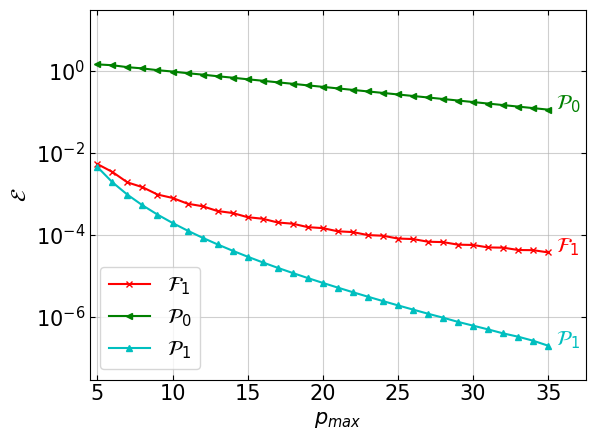
\includegraphics[width=.75\columnwidth]{plots/template_reconstruction_quadratic_sr.png}}\\
%\subfloat[Reconstructing the DBI Template]{\label{fig:b}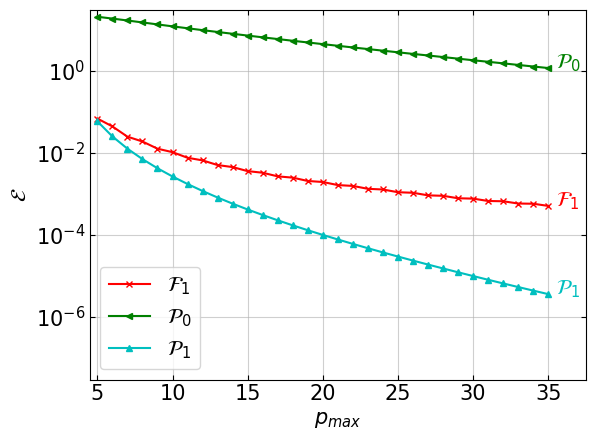
\includegraphics[width=.75\columnwidth]{plots/template_reconstruction_DBI.png}}
\subfloat[Reconstructing the Maldacena Template]{\label{fig:recon_a}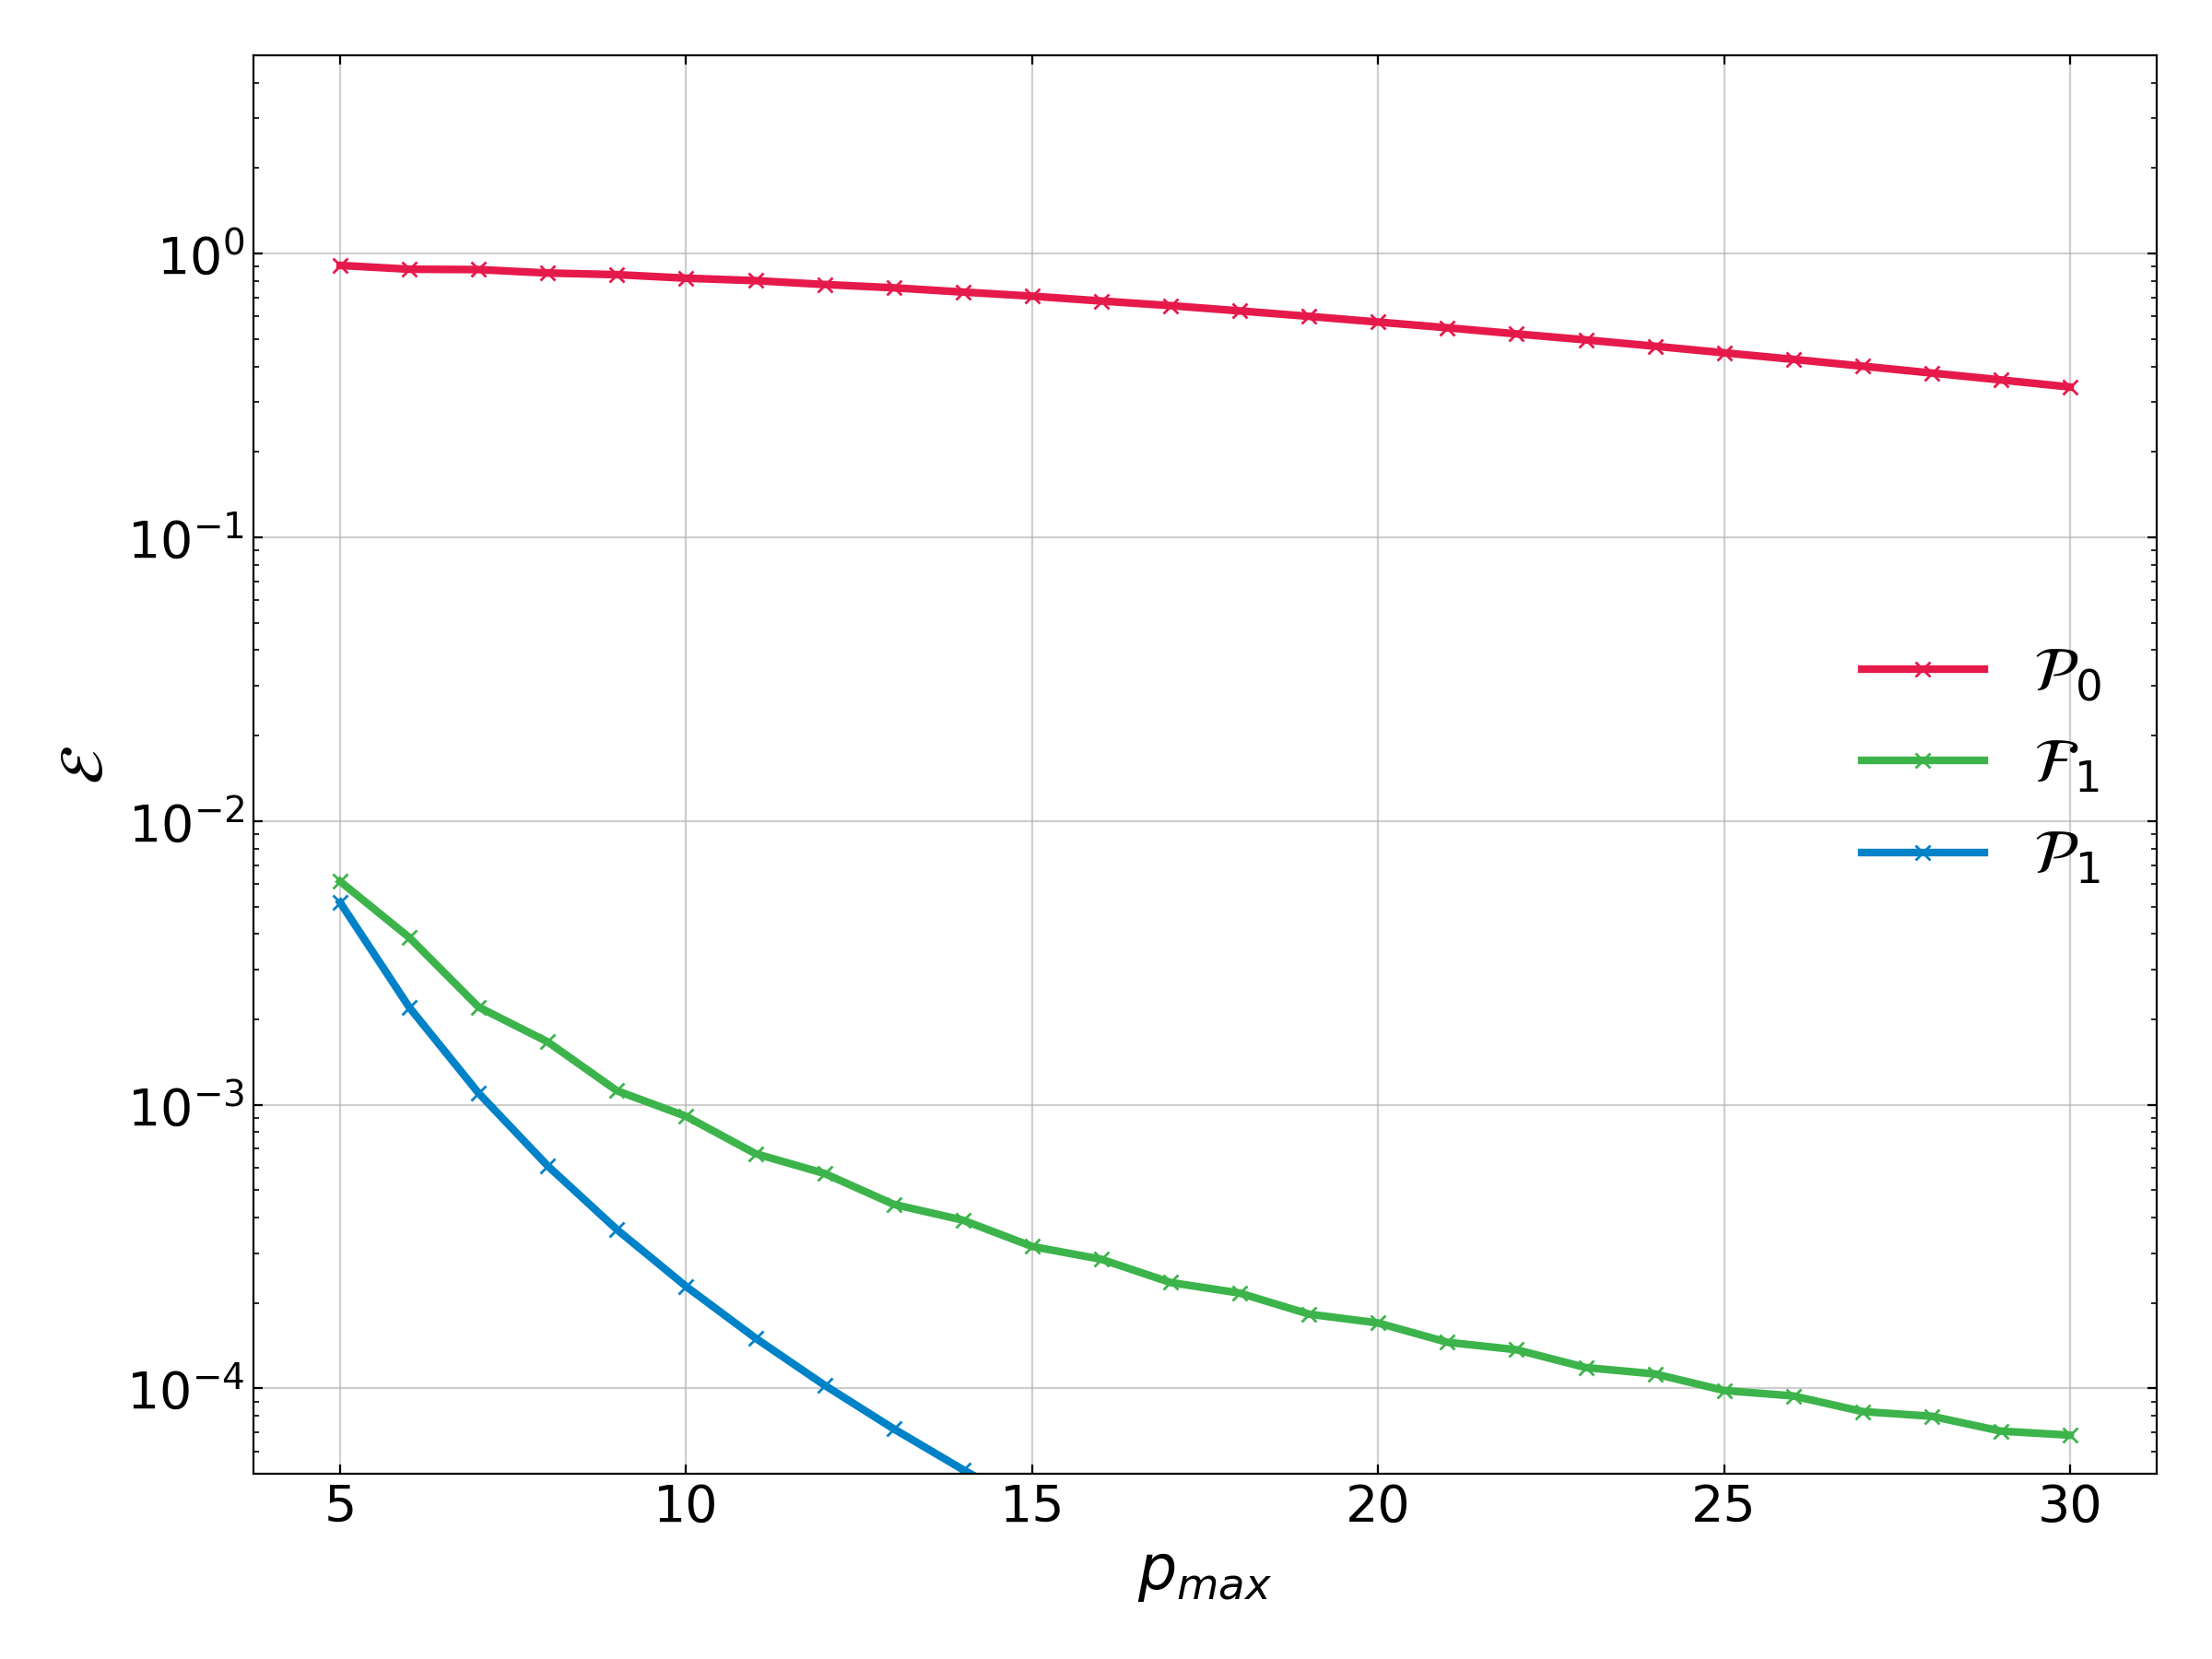
\includegraphics[width=.75\columnwidth]{pmax_reduction_plots_1_1000/malda.png}}\\
\subfloat[Reconstructing the DBI Template]{\label{fig:recon_b}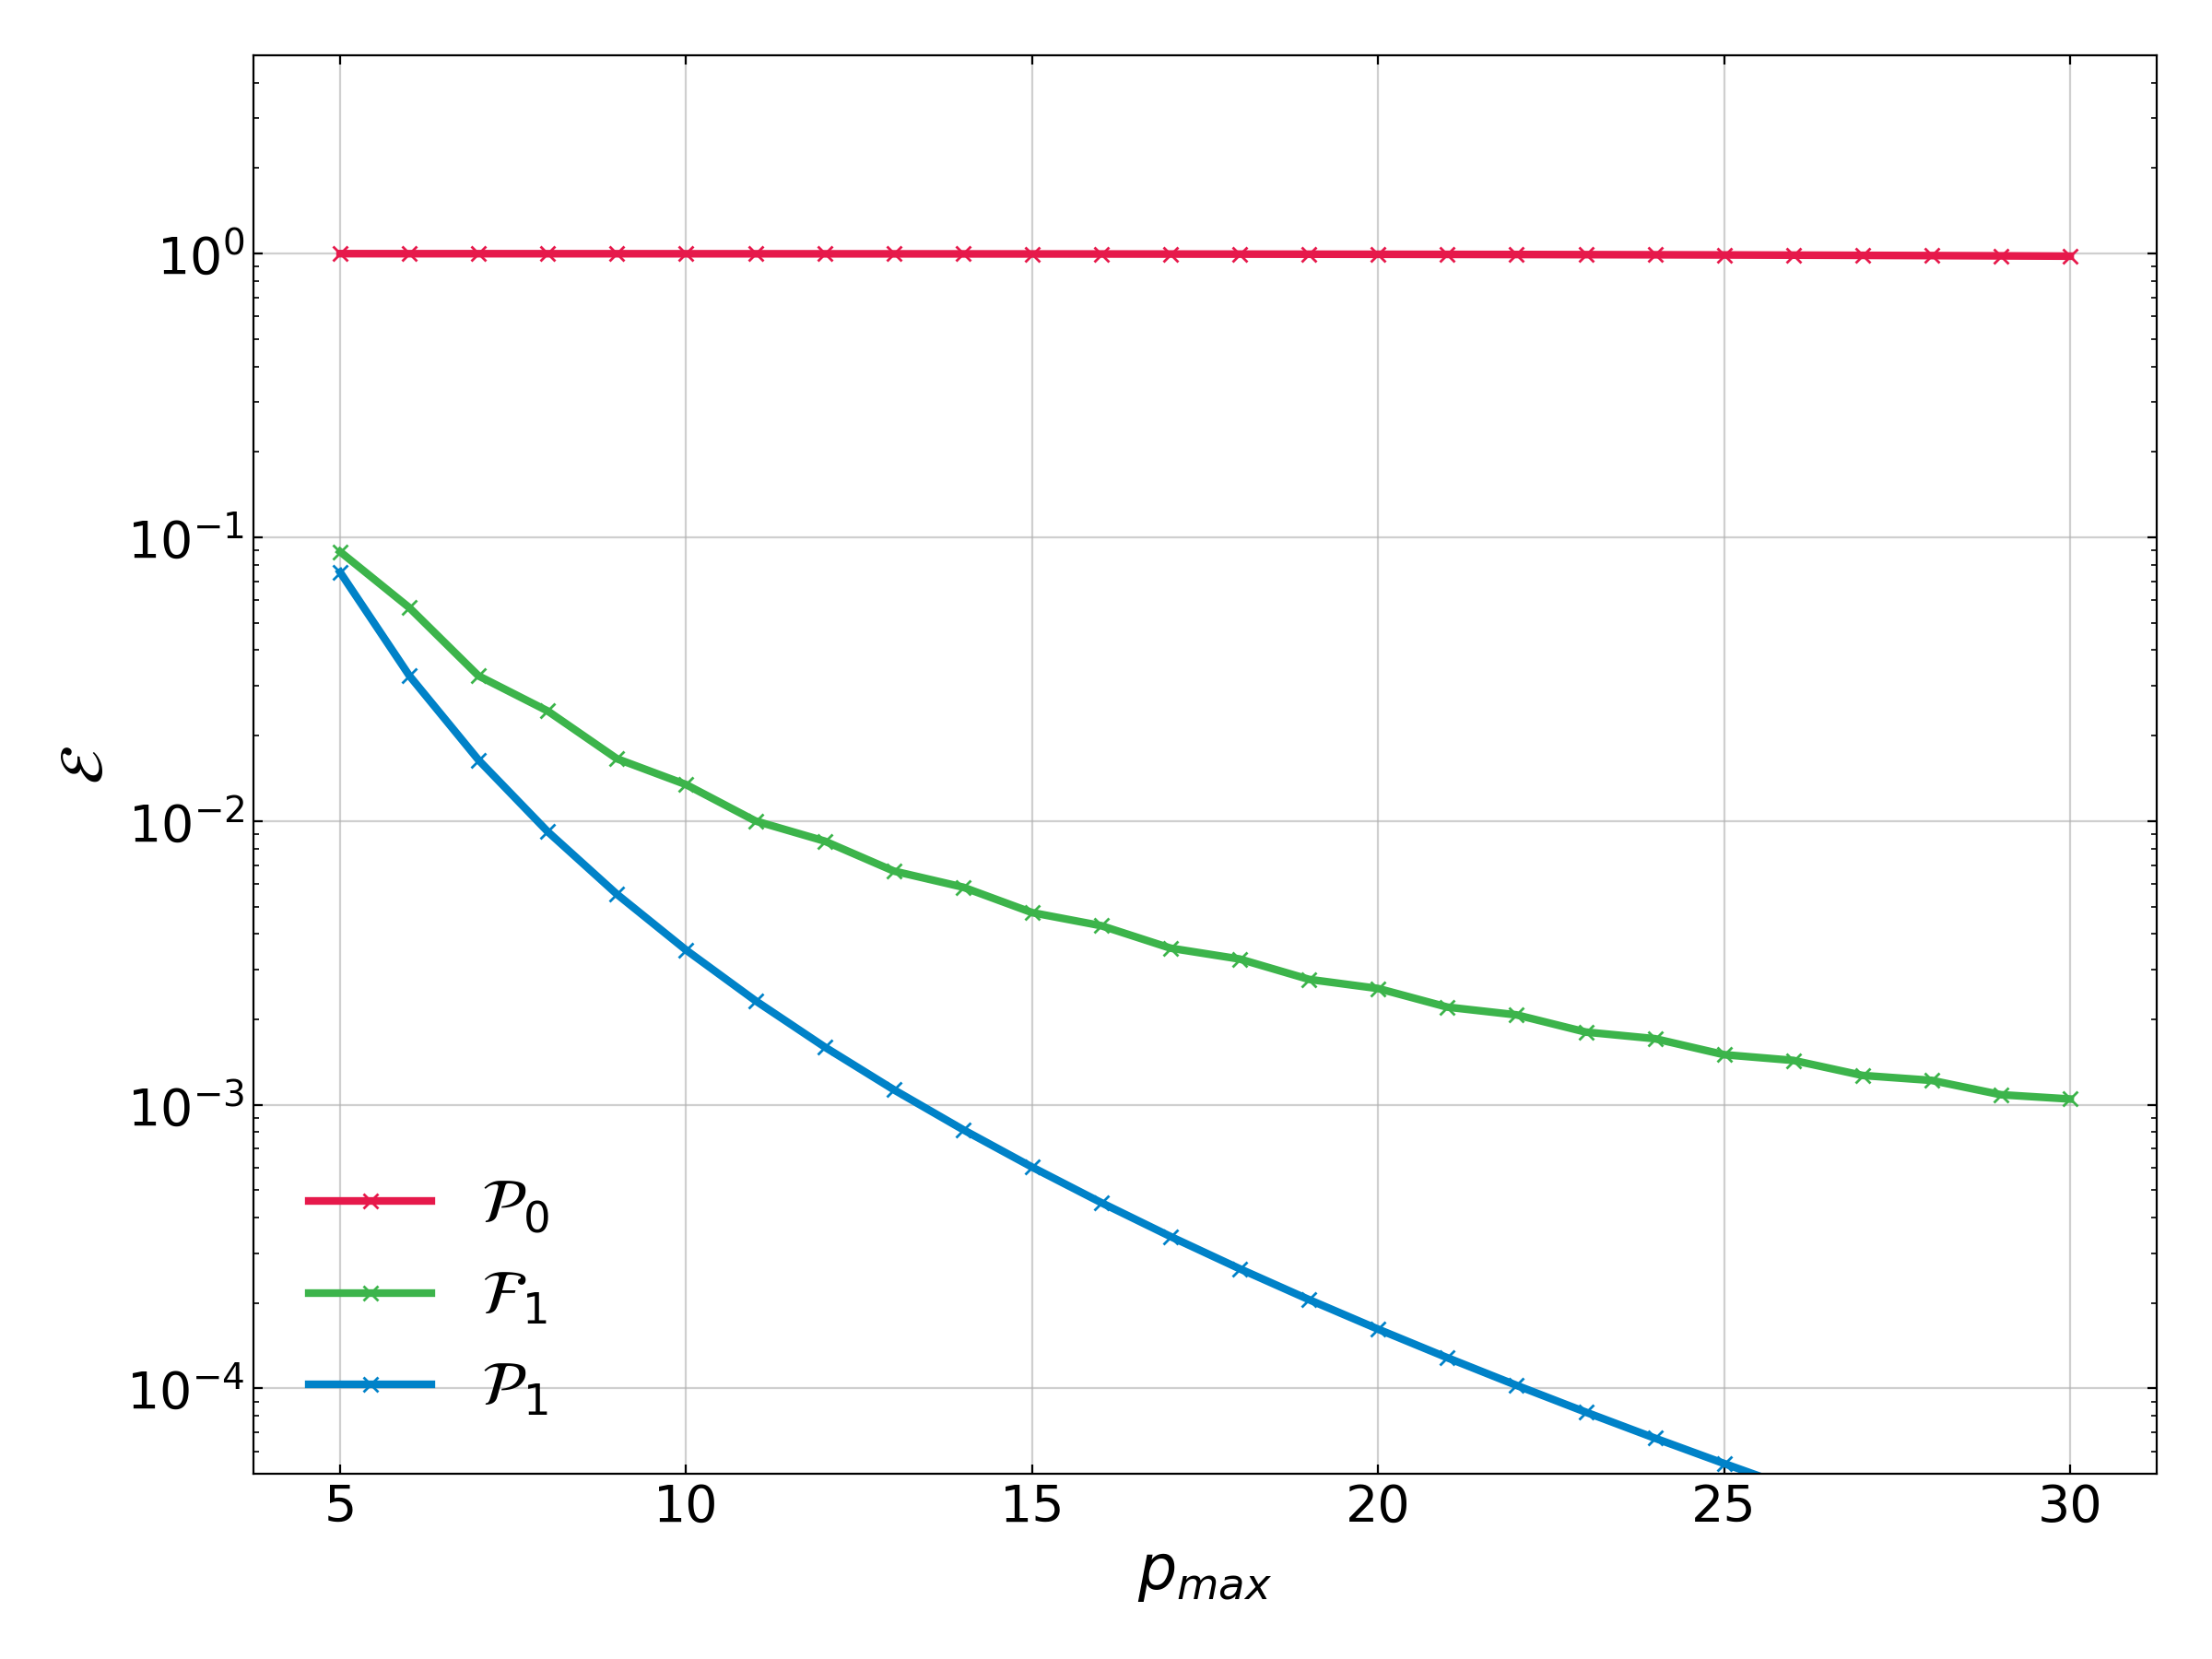
\includegraphics[width=.75\columnwidth]{pmax_reduction_plots_1_1000/dbi.png}}
\caption{
    Convergence comparisons for the Legendre and Fourier basis functions for (a) the Maldacena 
    template~\eqref{malda_shape} and (b) the DBI template~\eqref{dbi_shape}.
    The pure Legendre $\Lbasic$ basis requires many terms to fit the $1/k$ behaviour
    in both Maldacena's template~\eqref{malda_shape} and the $\dbi$ template~\eqref{dbi_shape}.
    In contrast, the $\Linvk$ basis (with an orthogonalised $1/k$ term) mitigates this dramatically, with the 
    error already reduced by a factor of $100$ at $\Pmax=5$.
    The Fourier $\Finvk$ basis performs well, but converges more slowly than the $\Linvk$ basis.
    Note that the convergence errors for~\eqref{dbi_shape} are larger than~\eqref{malda_shape} because of the larger contributions outside the tetrapyd dominating the fit.
    In this plot and the following, unless otherwise stated, $\kmax=1000\kmin$.
}\label{fig:recon_malda_dbi}
\end{figure}


Next, we investigate oscillatory model templates.
The simple feature model~\eqref{cos_shape} and the resonance model~\eqref{ln_cos_shape}
have scale dependence, but no shape dependence (in that they only depend on the perimeter
of the triangle, $K=k_1+k_2+k_3$).
We test our sets of basis functions on these two shapes,
and also when they are multiplied by~\eqref{dbi_shape} to obtain a feature
template with both shape and scale dependence.
As shown in Figure~\ref{fig:recon_osc_dbiosc},
$\Fbasic$ naturally outperform the basis sets built from Legendre modes for a pure oscillation.
However when the equilateral-type $\dbi$ template~\eqref{dbi_shape} is superimposed, even the augmented Fourier modes
$\Finvk$ converge poorly. Instead, the basis sets built from Legendre modes offer a more robust option,
with the $\scalingbasis$ basis performing best.
In Figure~\ref{fig:log_recon_osc_dbiosc} we see that for a logarithmic
oscillation, the $\resobasis$ basis converges in the fewest modes.


\begin{figure}[!pth]
\centering     %%% not \center
%\subfloat[$\cos(f(k_1+k_2+k_3))$]{\label{fig:a}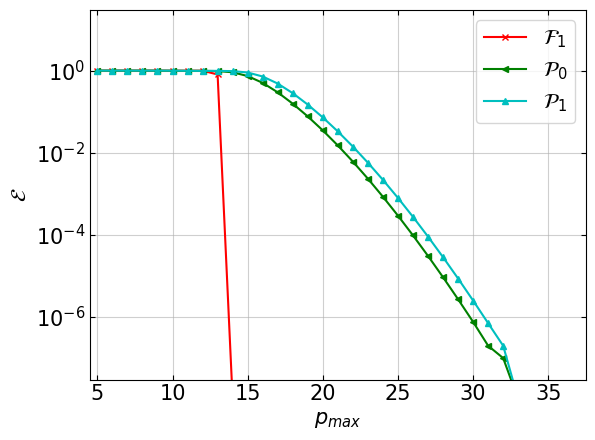
\includegraphics[width=.75\columnwidth]{plots/template_reconstruction_osc5.png}}\\
%\subfloat[$\cos(f(k_1+k_2+k_3))S^{DBI}$]{\label{fig:a}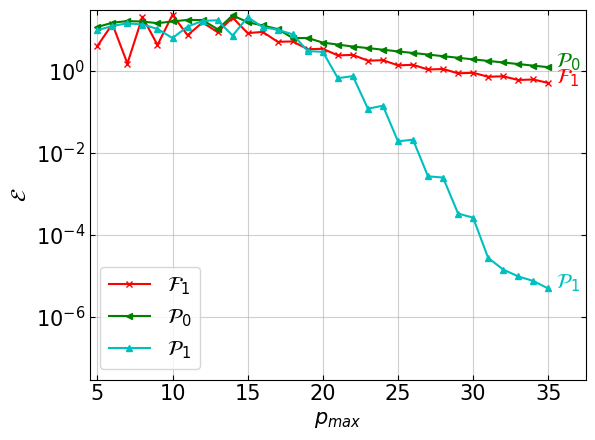
\includegraphics[width=.75\columnwidth]{plots/template_reconstruction_DBI_osc5.png}}
\subfloat[$\cos(f(k_1+k_2+k_3))$]{\label{fig:reduction_a}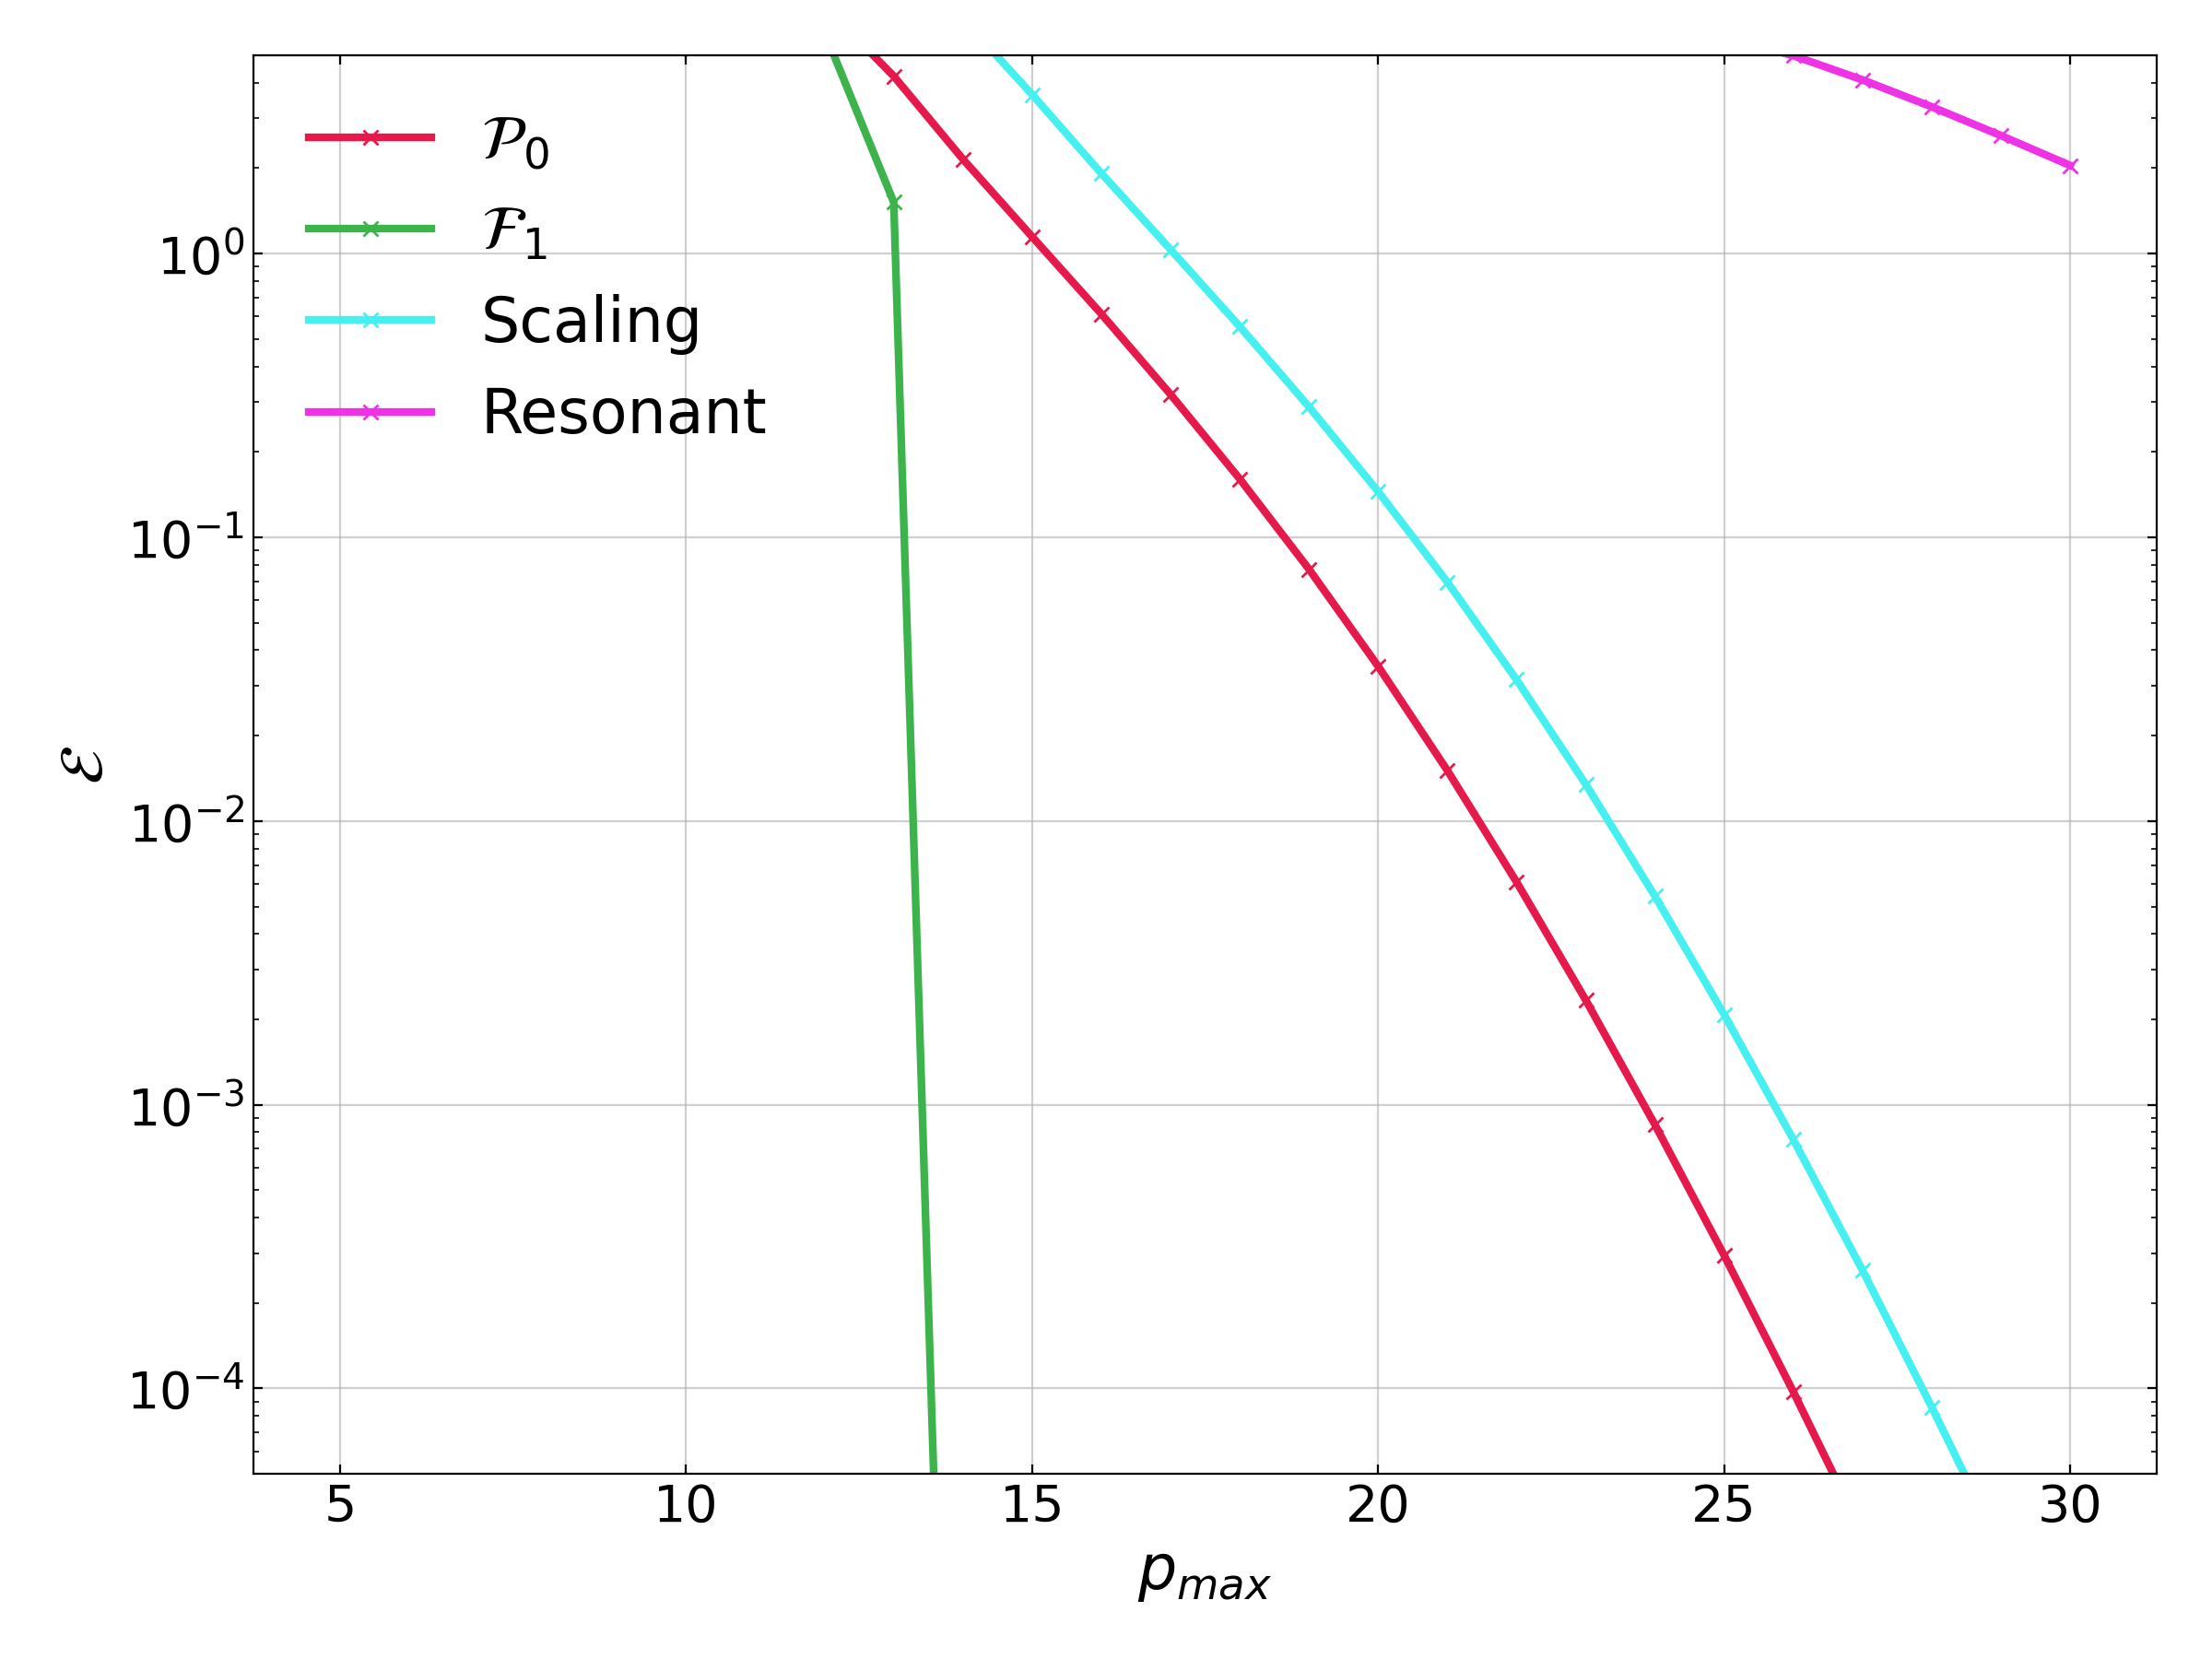
\includegraphics[width=.75\columnwidth]{pmax_reduction_plots_1_1000/cos15.png}}\\
\subfloat[$\cos(f(k_1+k_2+k_3))S^{DBI}$]{\label{fig:reduction_b}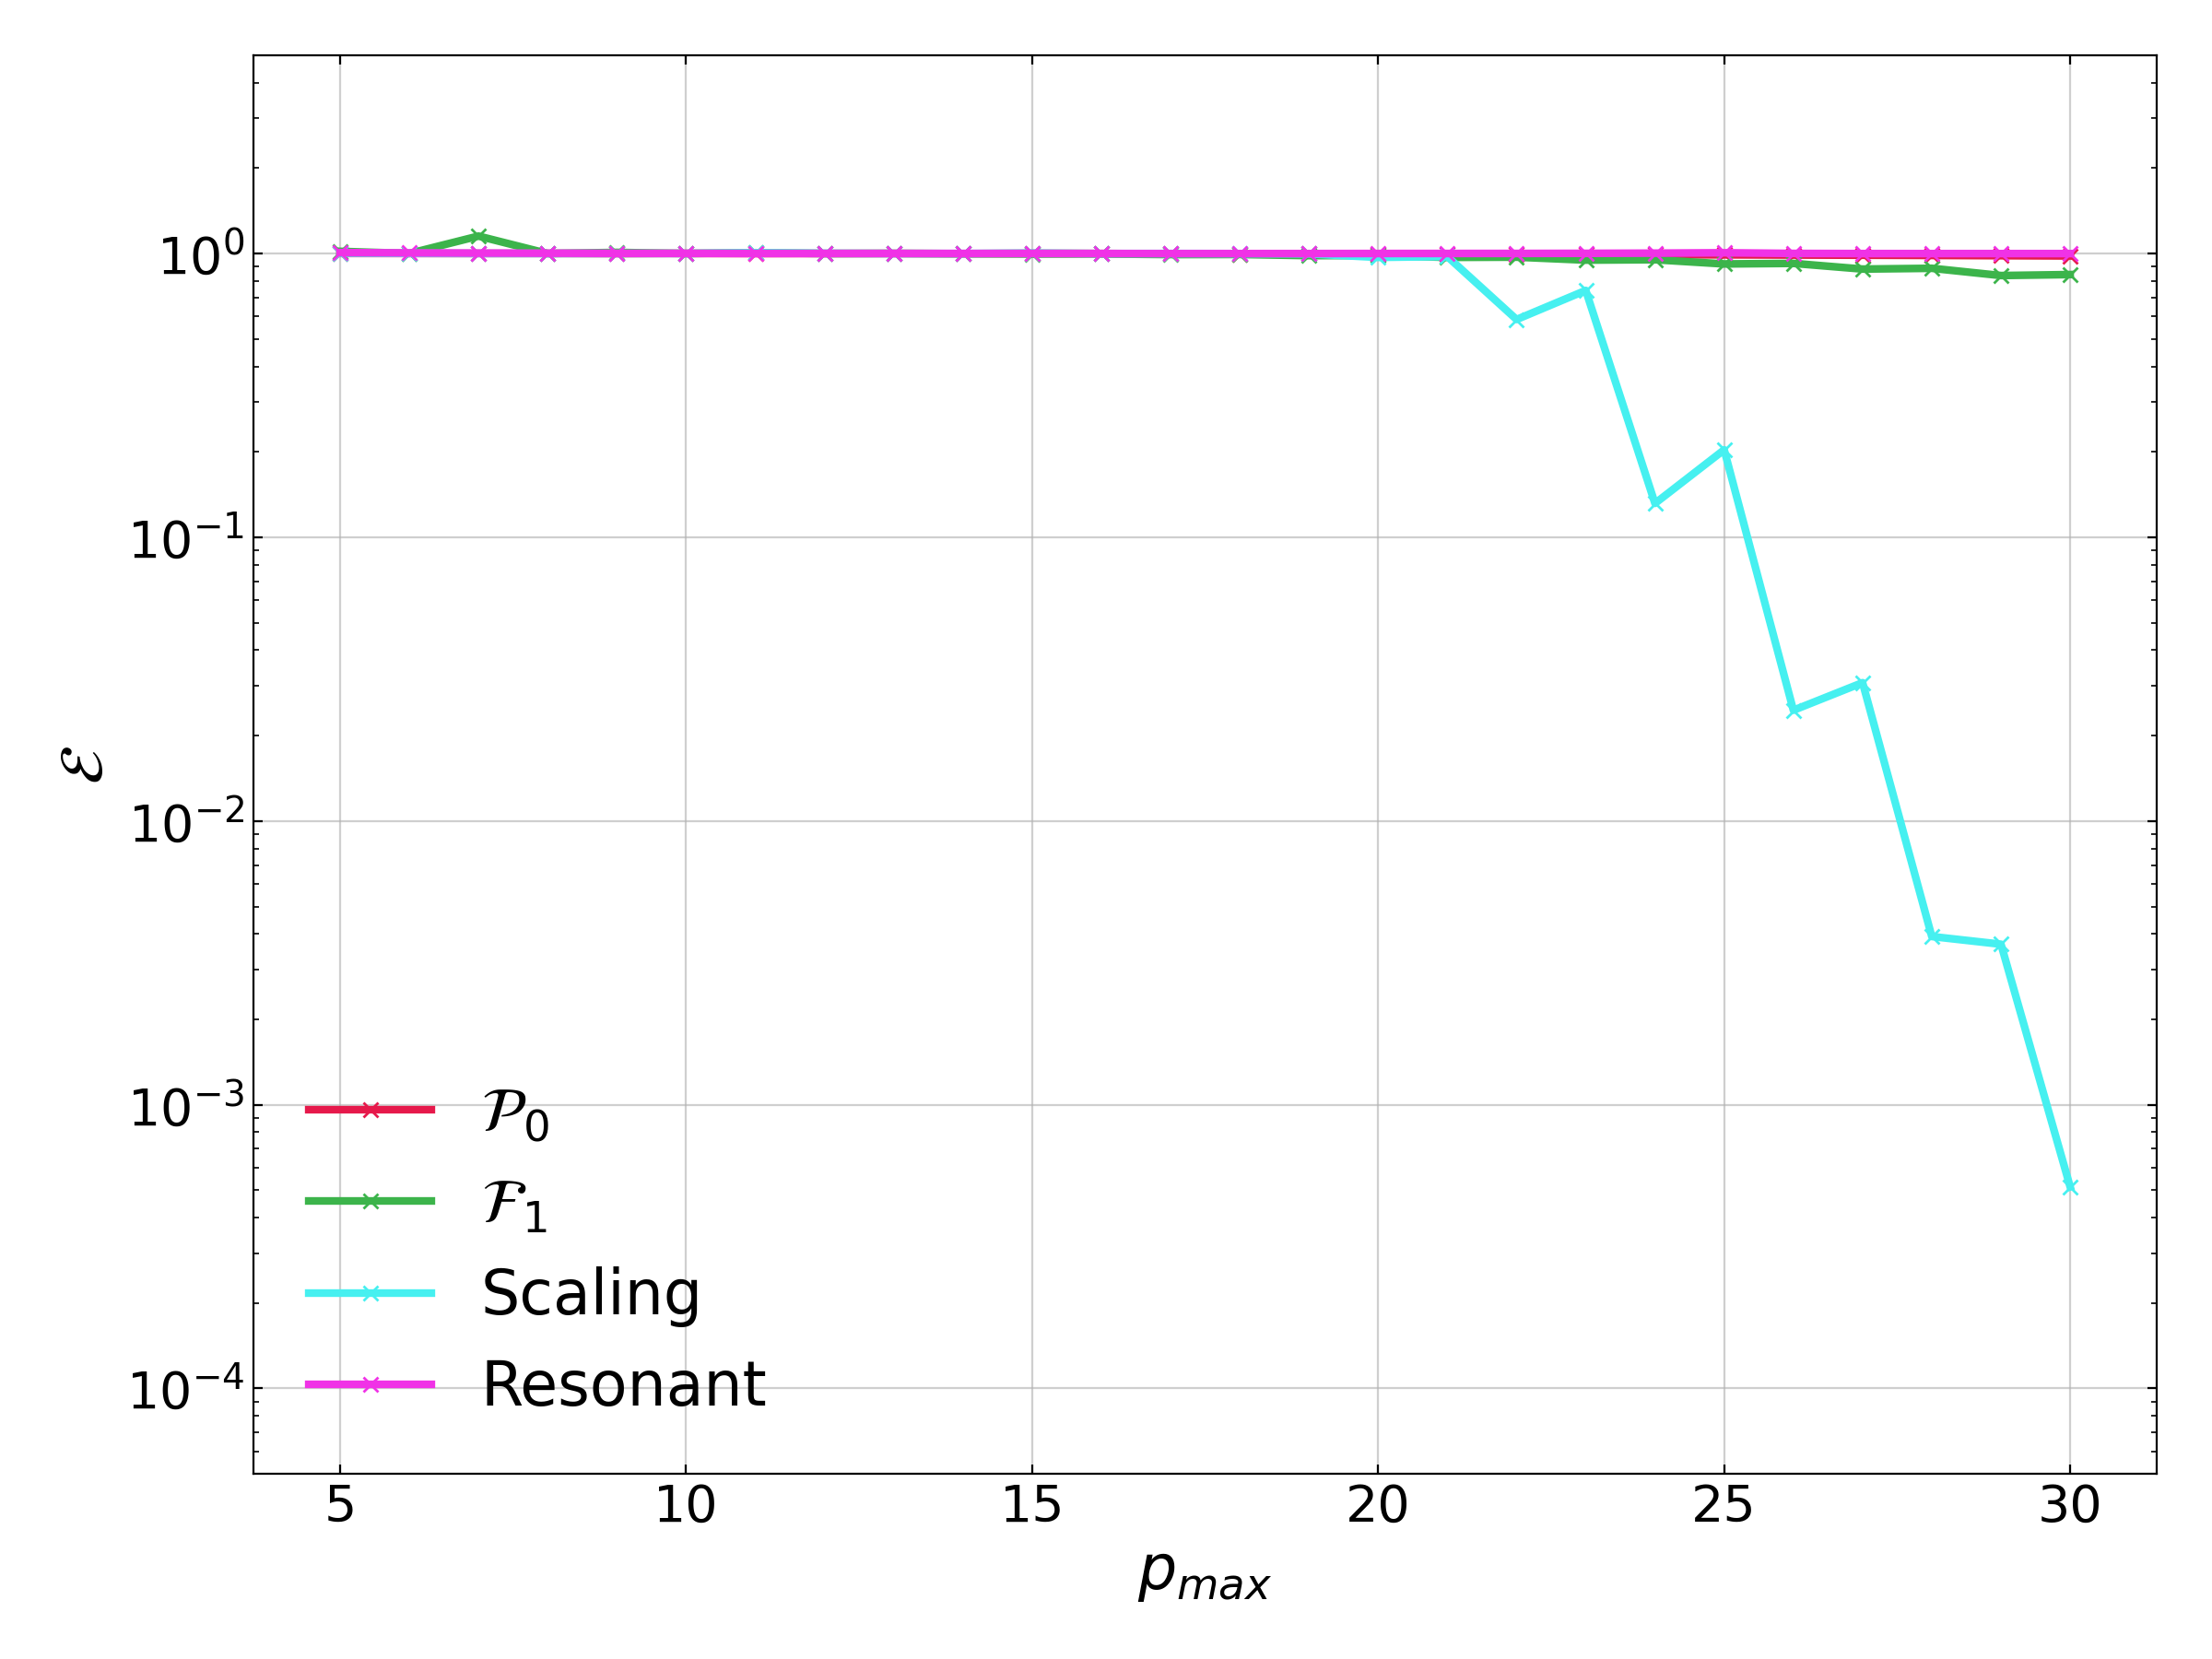
\includegraphics[width=.75\columnwidth]{pmax_reduction_plots_1_1000/dbi_cos15.png}}
\caption{
    Convergence comparison for oscillatory models.
    For linear oscillations we choose $f=150.64$ (so we obtain $15$ whole oscillations in the $k$-range).
    (a) As expected, the $\Finvk$ basis fits an oscillation with
    no shape dependence~\eqref{cos_shape} (that is periodic in the $k$-range) perfectly.
    For this special case, the $\Lbasic$, $\scalingbasis$ and $\resobasis$ sets of basis functions require more modes
    to accurately describe the shape. (b) However, moving to the more complex and realistic case of a
    feature with scale and shape dependence (in this case the product of~\eqref{dbi_shape}
    and~\eqref{cos_shape}), we see that again the $\scalingbasis$ basis converges with the fewest modes.
    Note that before the expansion has fully converged, the fit on the tetrapyd
    can actually degrade slightly when the basis set is extended. This is an artifact
    of fitting on the cube and restricting~\eqref{relative_difference}
    to the physical configurations on the tetrapyd; when considered over the
    entire cube the fit improves monotonically.
    The $\resobasis$ basis, naturally, does not converge well to a linear oscillation.
}\label{fig:recon_osc_dbiosc}
\end{figure}
\begin{figure}[!pth]
\centering     %%% not \center
%\subfloat[$\cos(f\log(k_1+k_2+k_3))$]{\label{fig:a}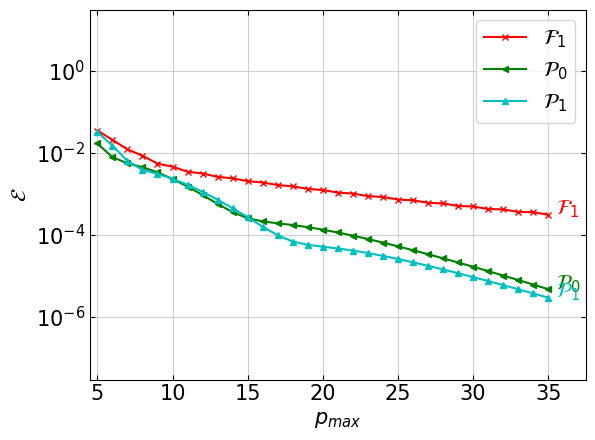
\includegraphics[width=.75\columnwidth]{plots/template_reconstruction_logosc2.png}}\\
%\subfloat[$\cos(f\log(k_1+k_2+k_3))S^{DBI}$]{\label{fig:a}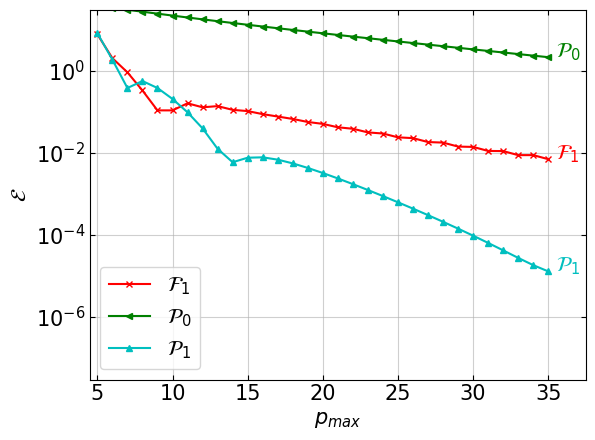
\includegraphics[width=.75\columnwidth]{plots/template_reconstruction_DBI_logosc2.png}}
\subfloat[$\cos(f\log(k_1+k_2+k_3))S^{DBI}$ on the tetrapyd]{\label{fig:reduction_c}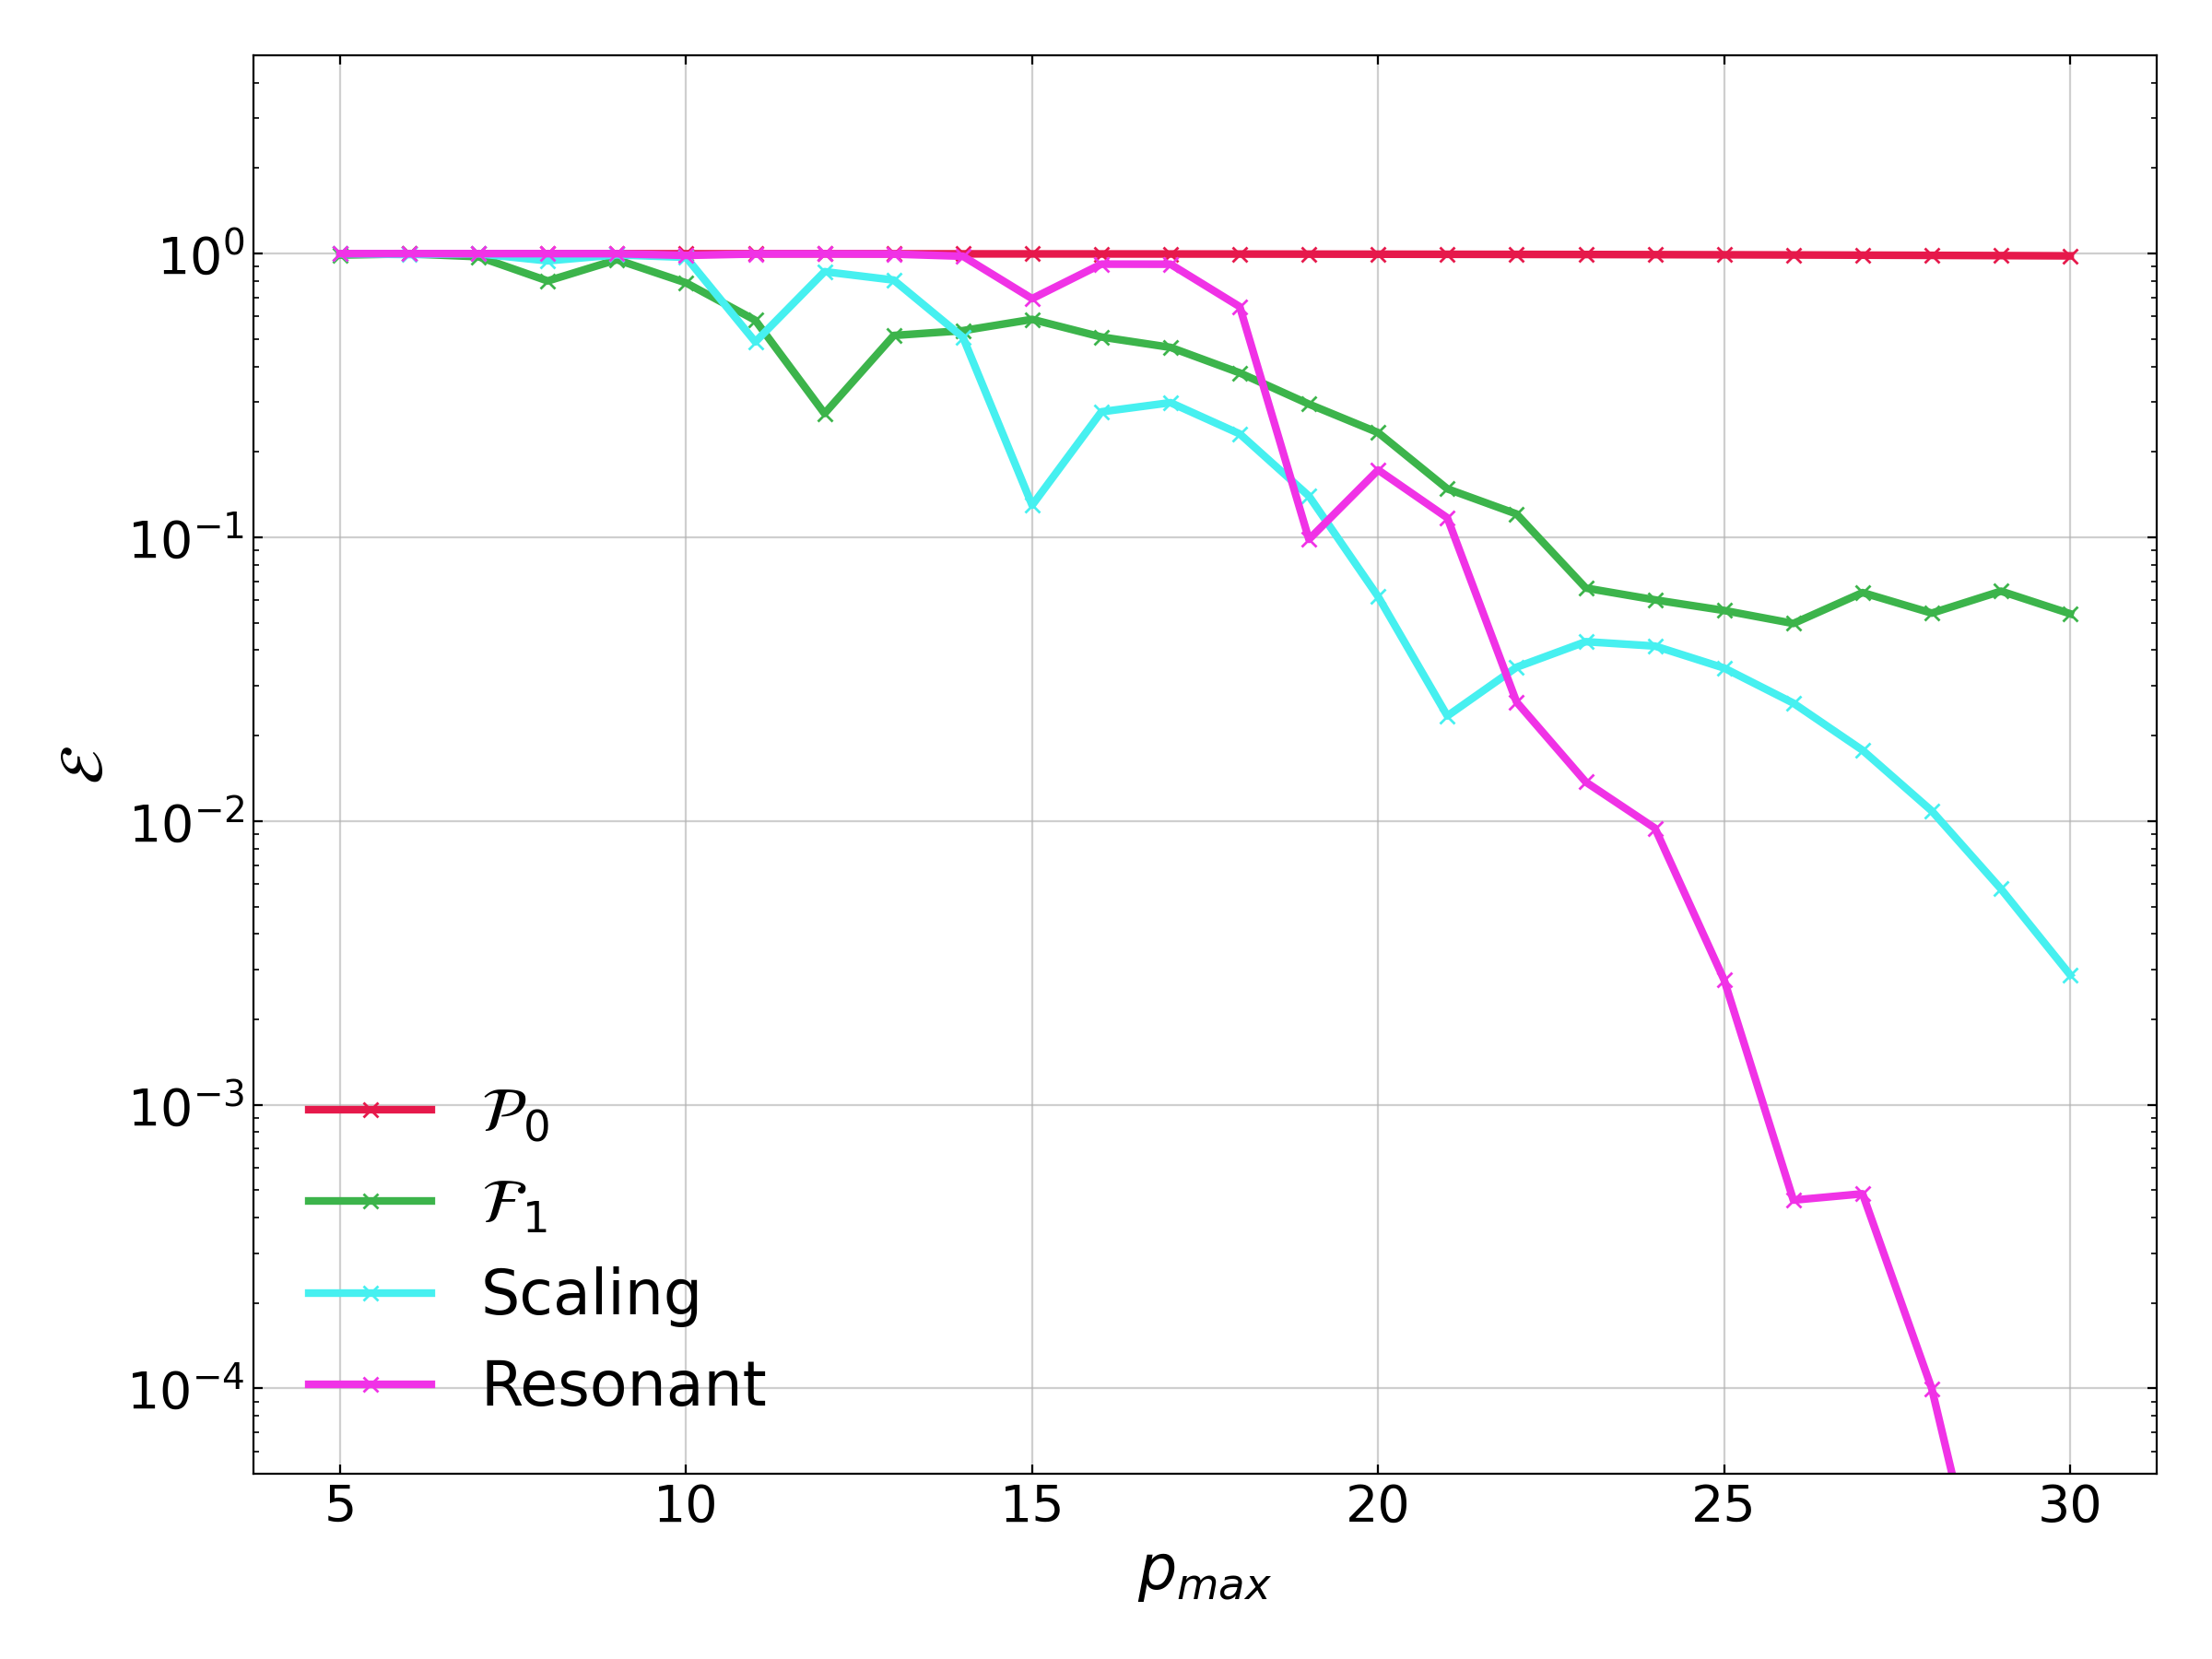
\includegraphics[width=.75\columnwidth]{pmax_reduction_plots_1_1000/dbi_cos5_log.png}}\\
\subfloat[$\cos(f\log(k_1+k_2+k_3))S^{DBI}$ on the cube]{\label{fig:reduction_ca}\includegraphics[width=.75\columnwidth]{pmax_cube_reduction_plots_1_1000/dbi_cos5_log_cube.png}}
\caption{
    %(a) The convergence for a log oscillation model~\eqref{ln_cos_shape} with no shape dependence.
    %For this type of feature, the $\Lbasic$ and $\Linvk$ sets of basis functions require fewer modes
    %to accurately describe the shape than the $\Finvk$ basis.
    %(b)
    %For the more complex and realistic case of a
    We plot the convergence of various basis sets for the more complex case of a resonant
    feature with scale and shape dependence, in this case the product of~\eqref{dbi_shape}
    and~\eqref{ln_cos_shape}.
    We choose $f=4.55$ (so we obtain $5$ whole oscillations in the $k$-range).
    (a) On the tetrapyd, we see that the $\scalingbasis$ basis struggles to converge for this fixed-frequency
    template, due to the combination of the high frequency logarithmic oscillation
    and the non-trivial shape dependence coming from $S^{DBI}(k_1,k_2,k_3)$.
    As expected for logarithmic oscillations,
    the $\resobasis$ basis performs best for this template, confirming that
    the basis functions defined in~\eqref{reso_basis_definition} perform well
    even when there is non-trivial shape dependence.
    (b) On the cube, we see that the results converge orders of magnitude faster---see
    discussion in Section~\ref{sec:large_non_physical}.
}\label{fig:log_recon_osc_dbiosc}
\end{figure}

\begin{figure}[!pth]
\centering
%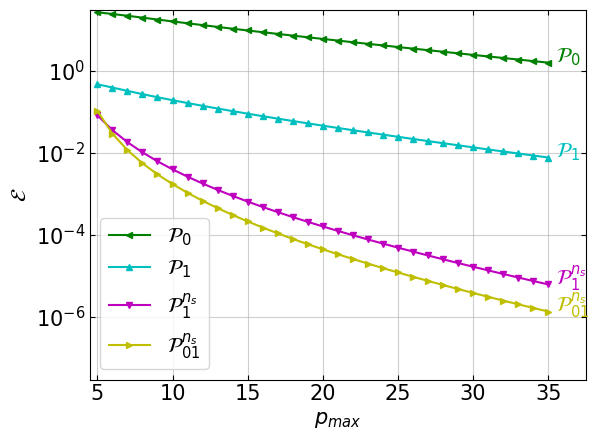
\includegraphics[width=0.8\columnwidth]{plots/template_reconstruction_DBI_ns.png}
%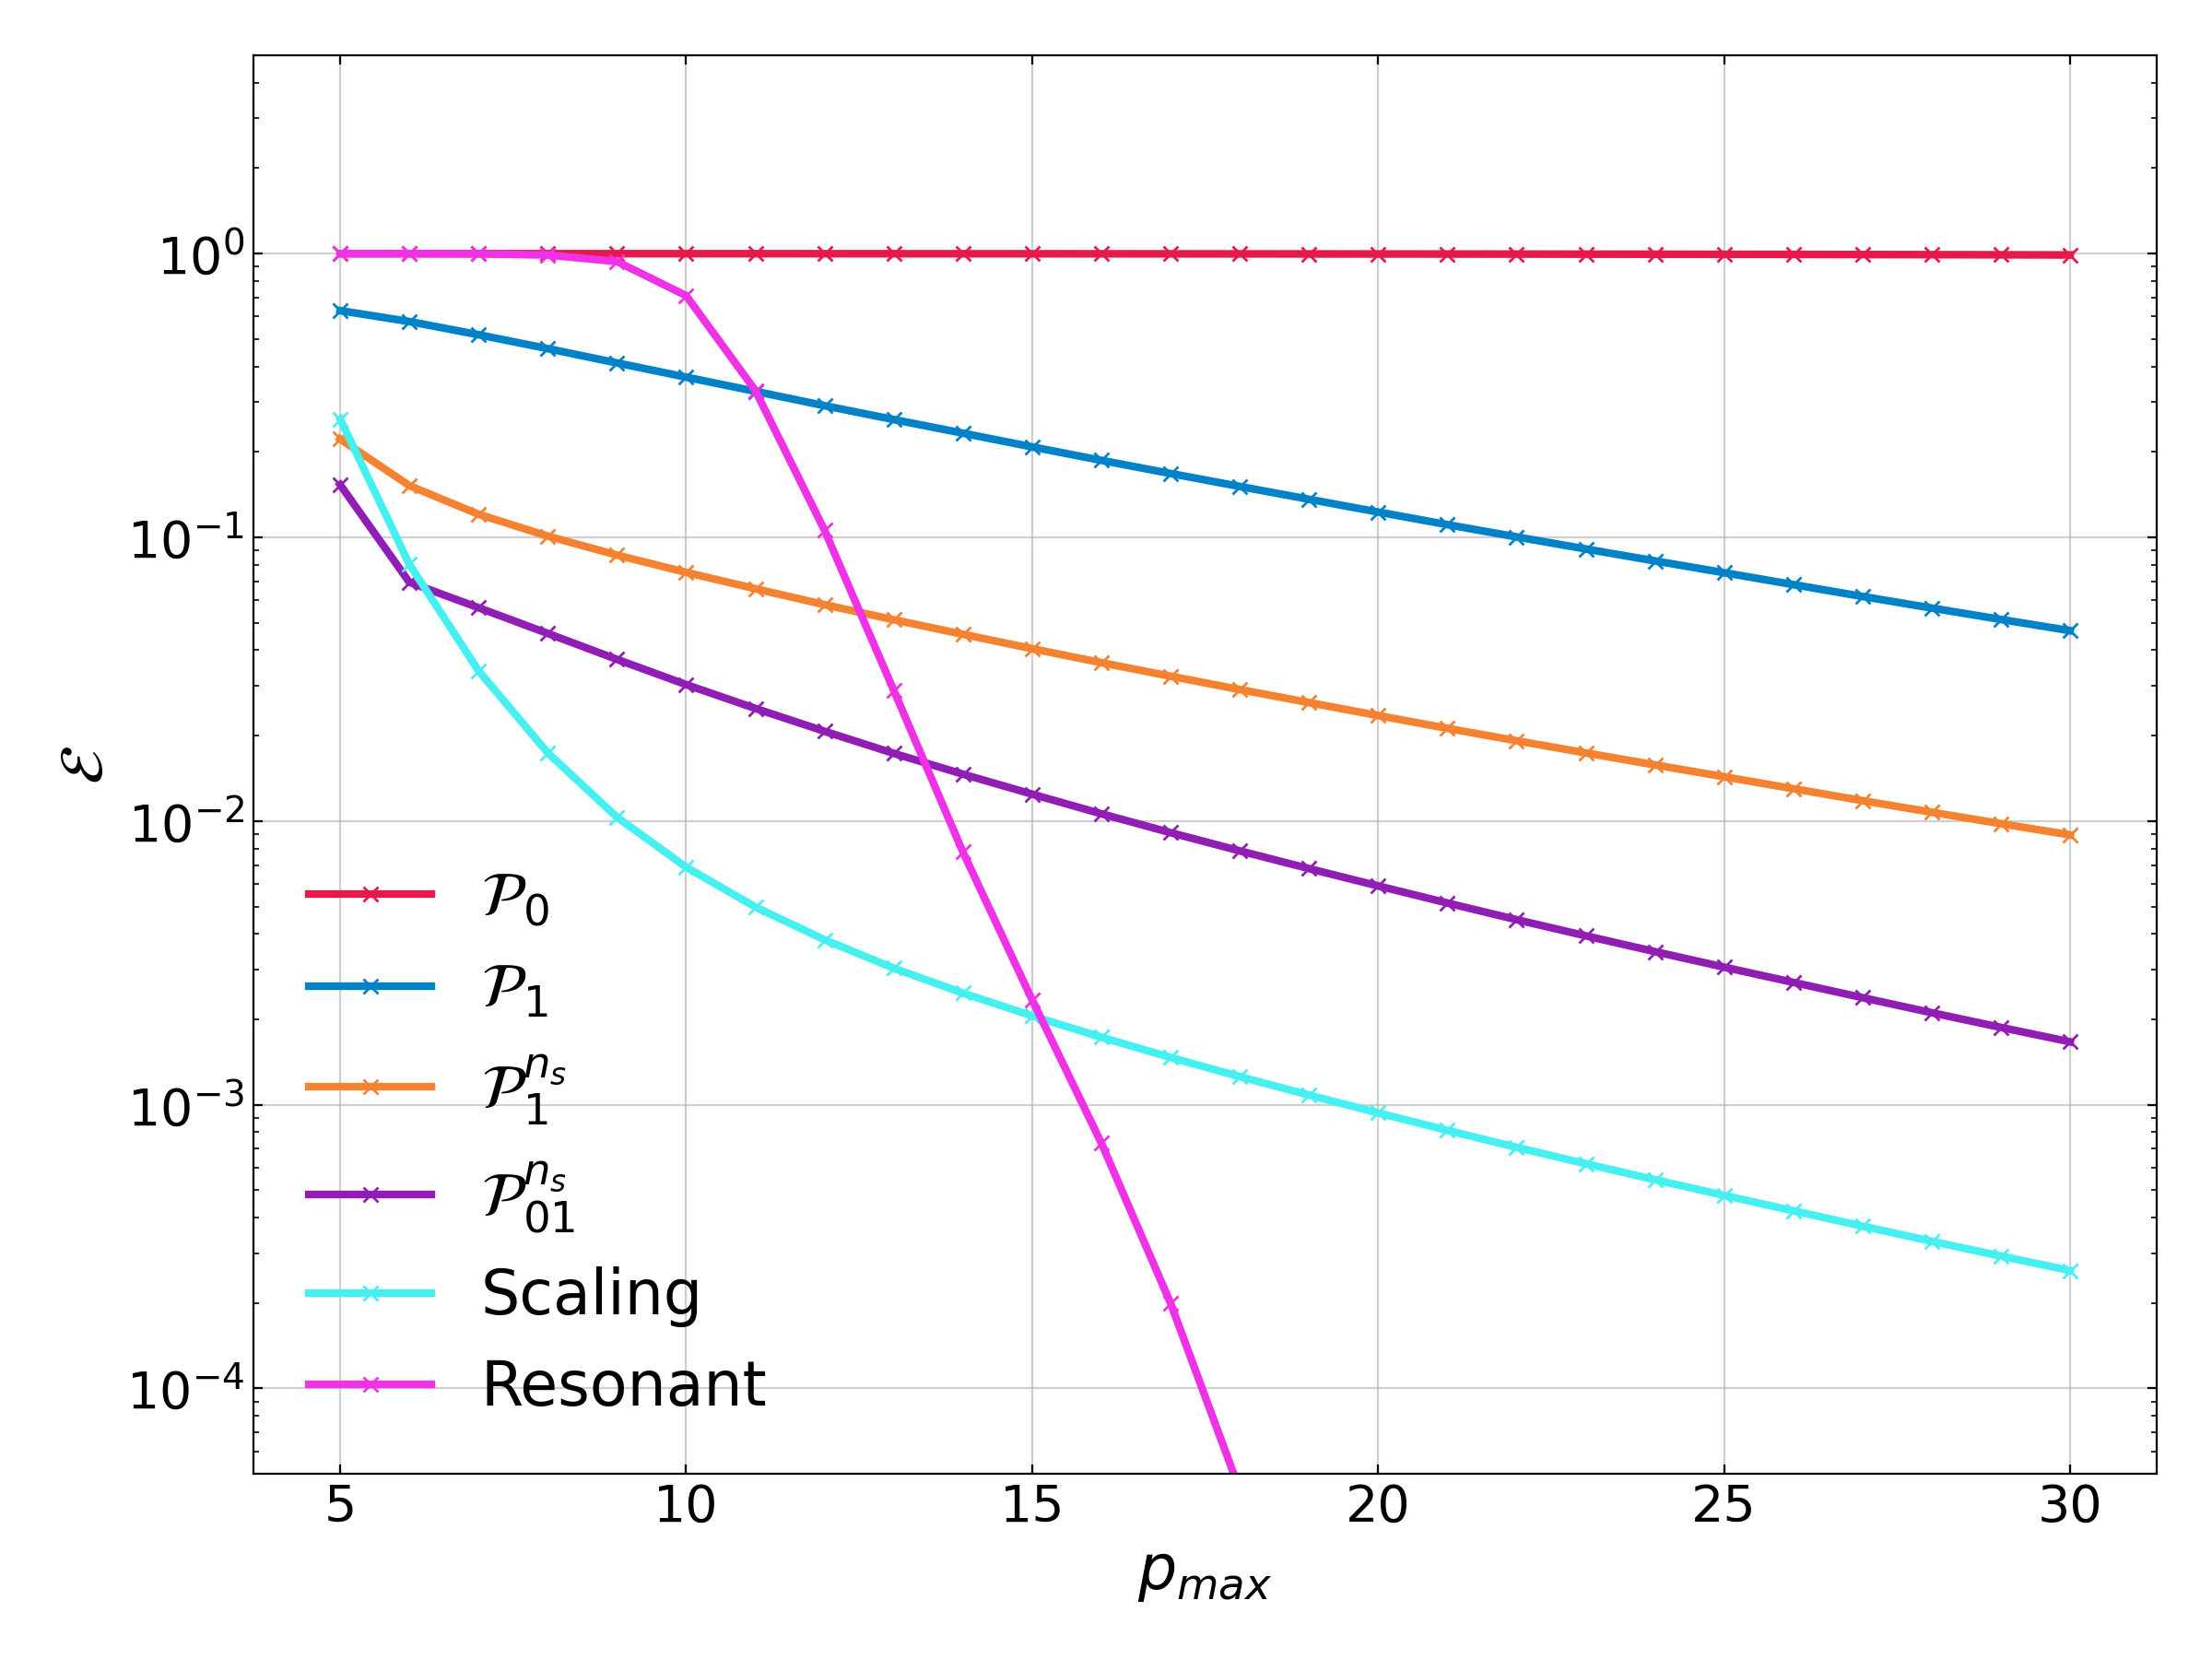
\includegraphics[width=0.8\columnwidth]{pmax_reduction_plots_1_1000/dbi_scaling.png}
\subfloat[$\kmax/\kmin=550$]{\label{fig:scale_550}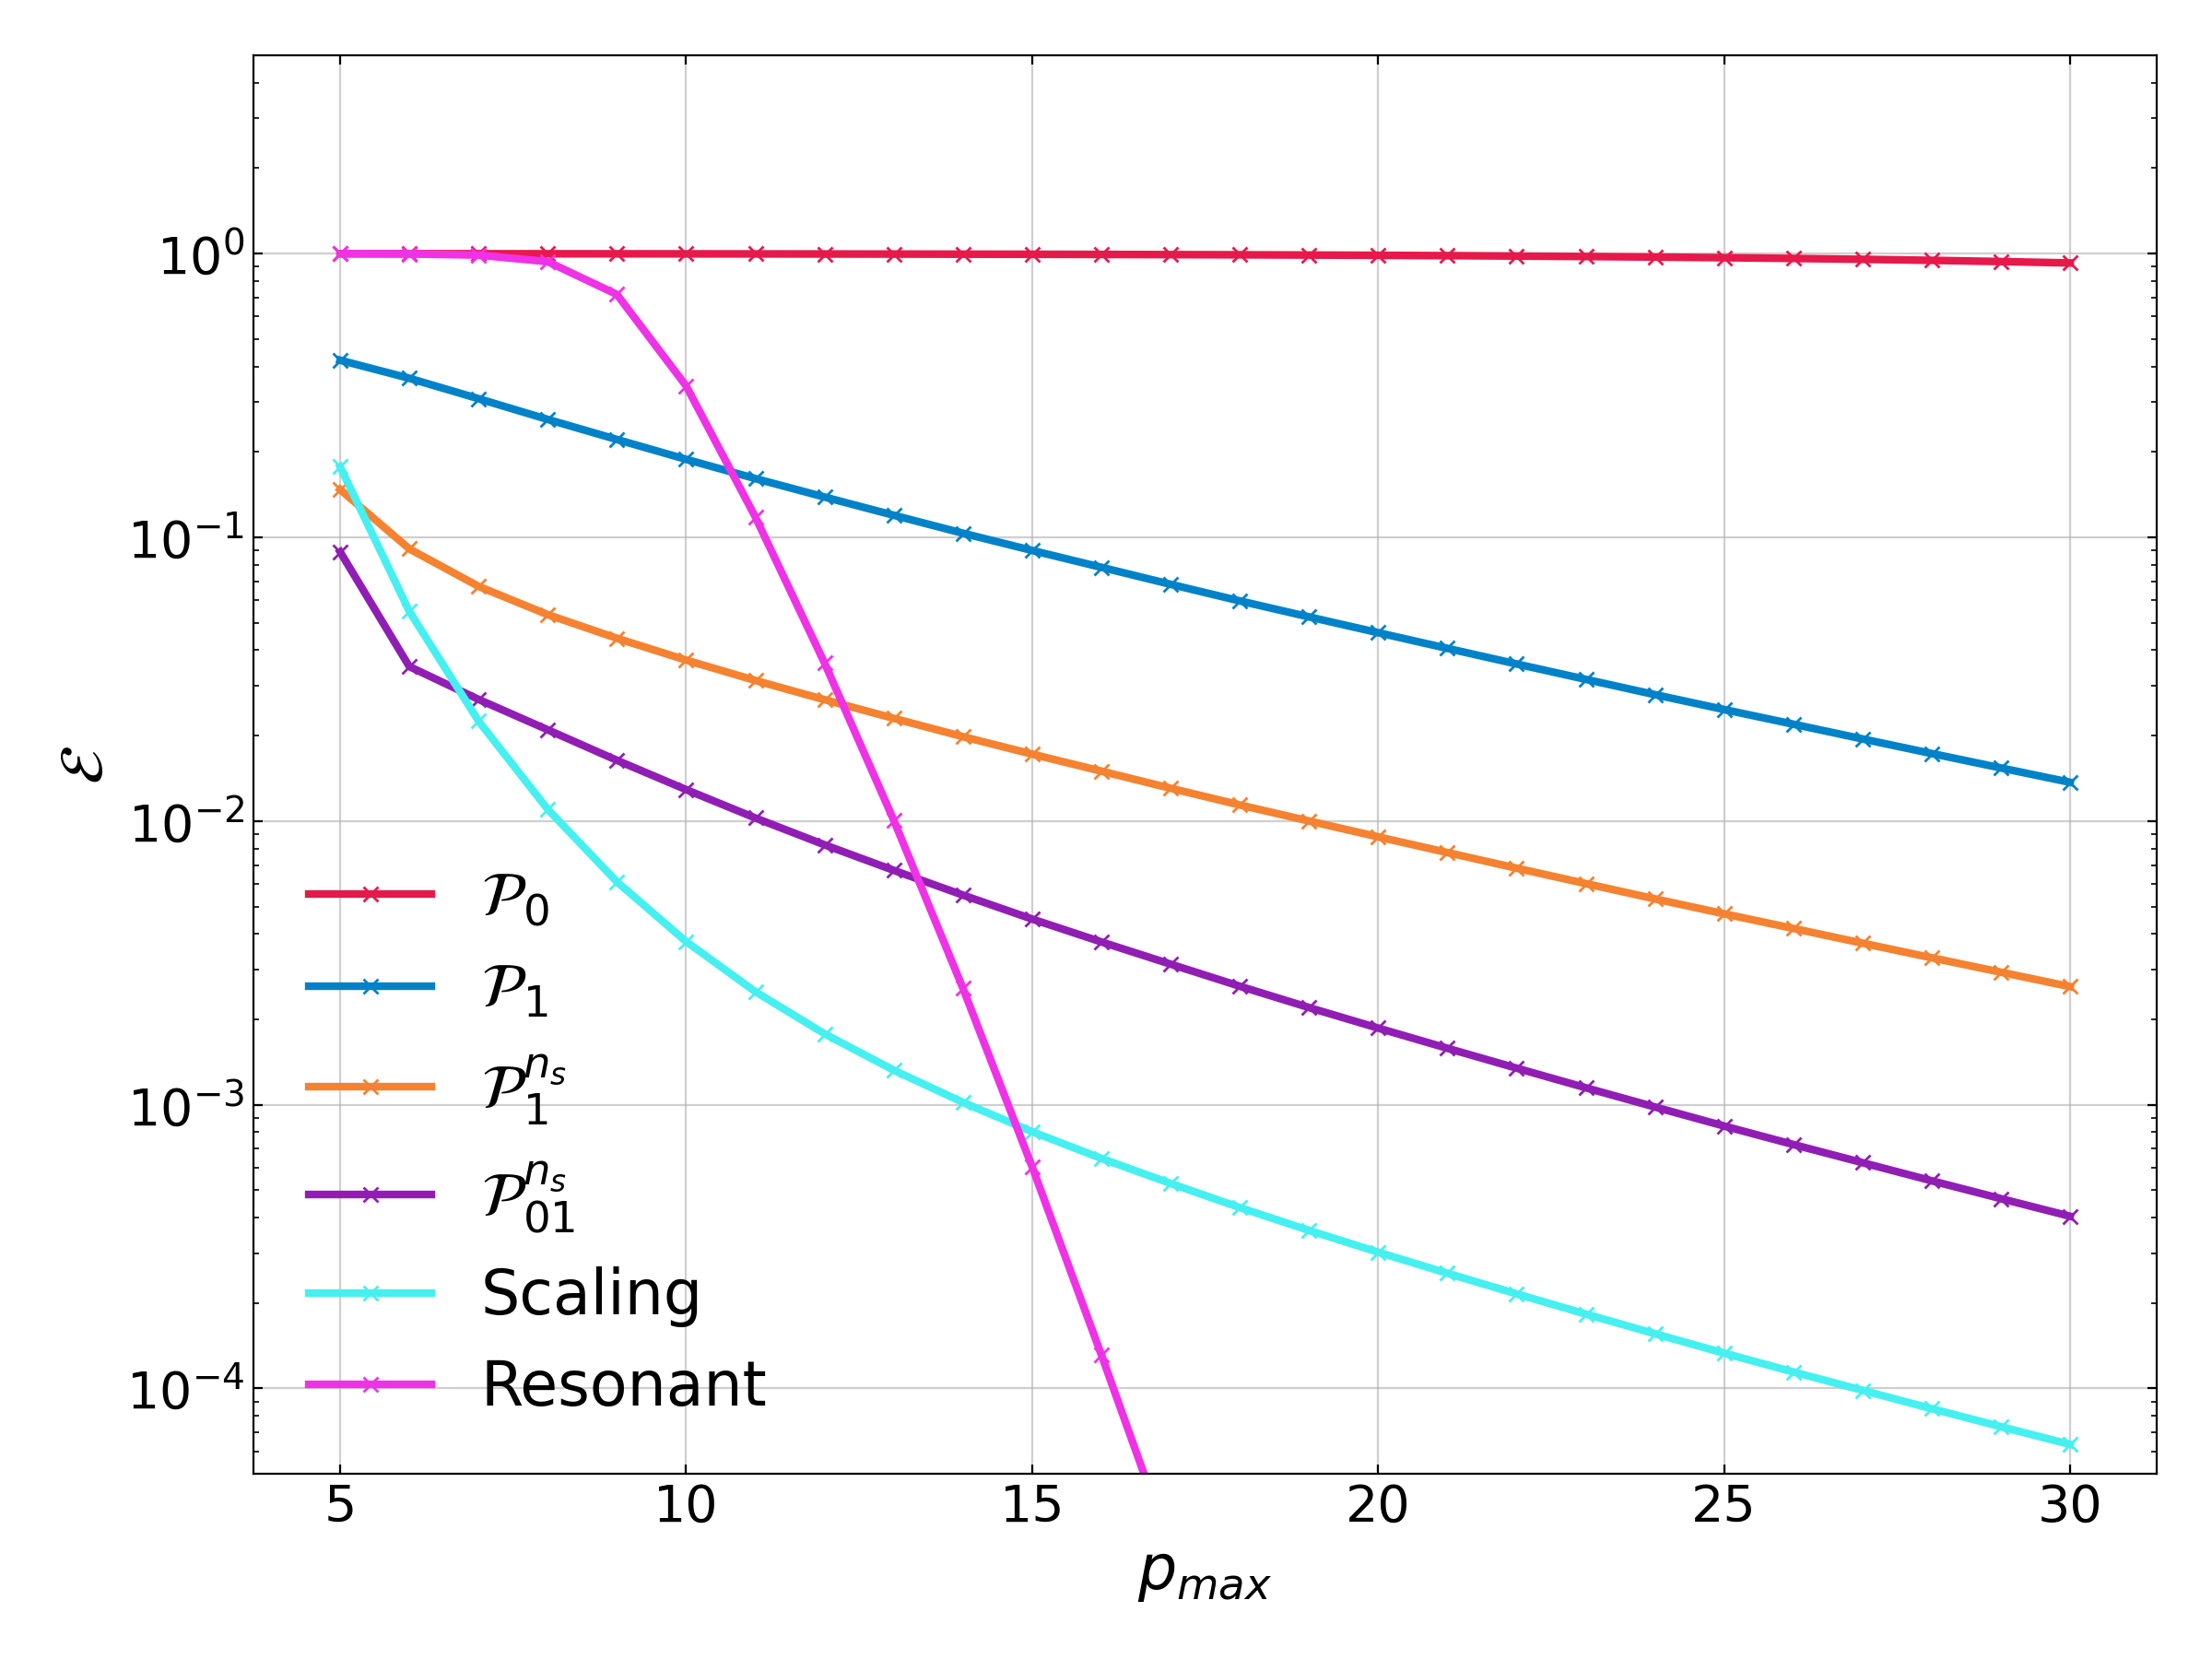
\includegraphics[width=.75\columnwidth]{pmax_reduction_plots_1_550/dbi_scaling.png}}\\
\subfloat[$\kmax/\kmin=1000$]{\label{fig:scale_1000}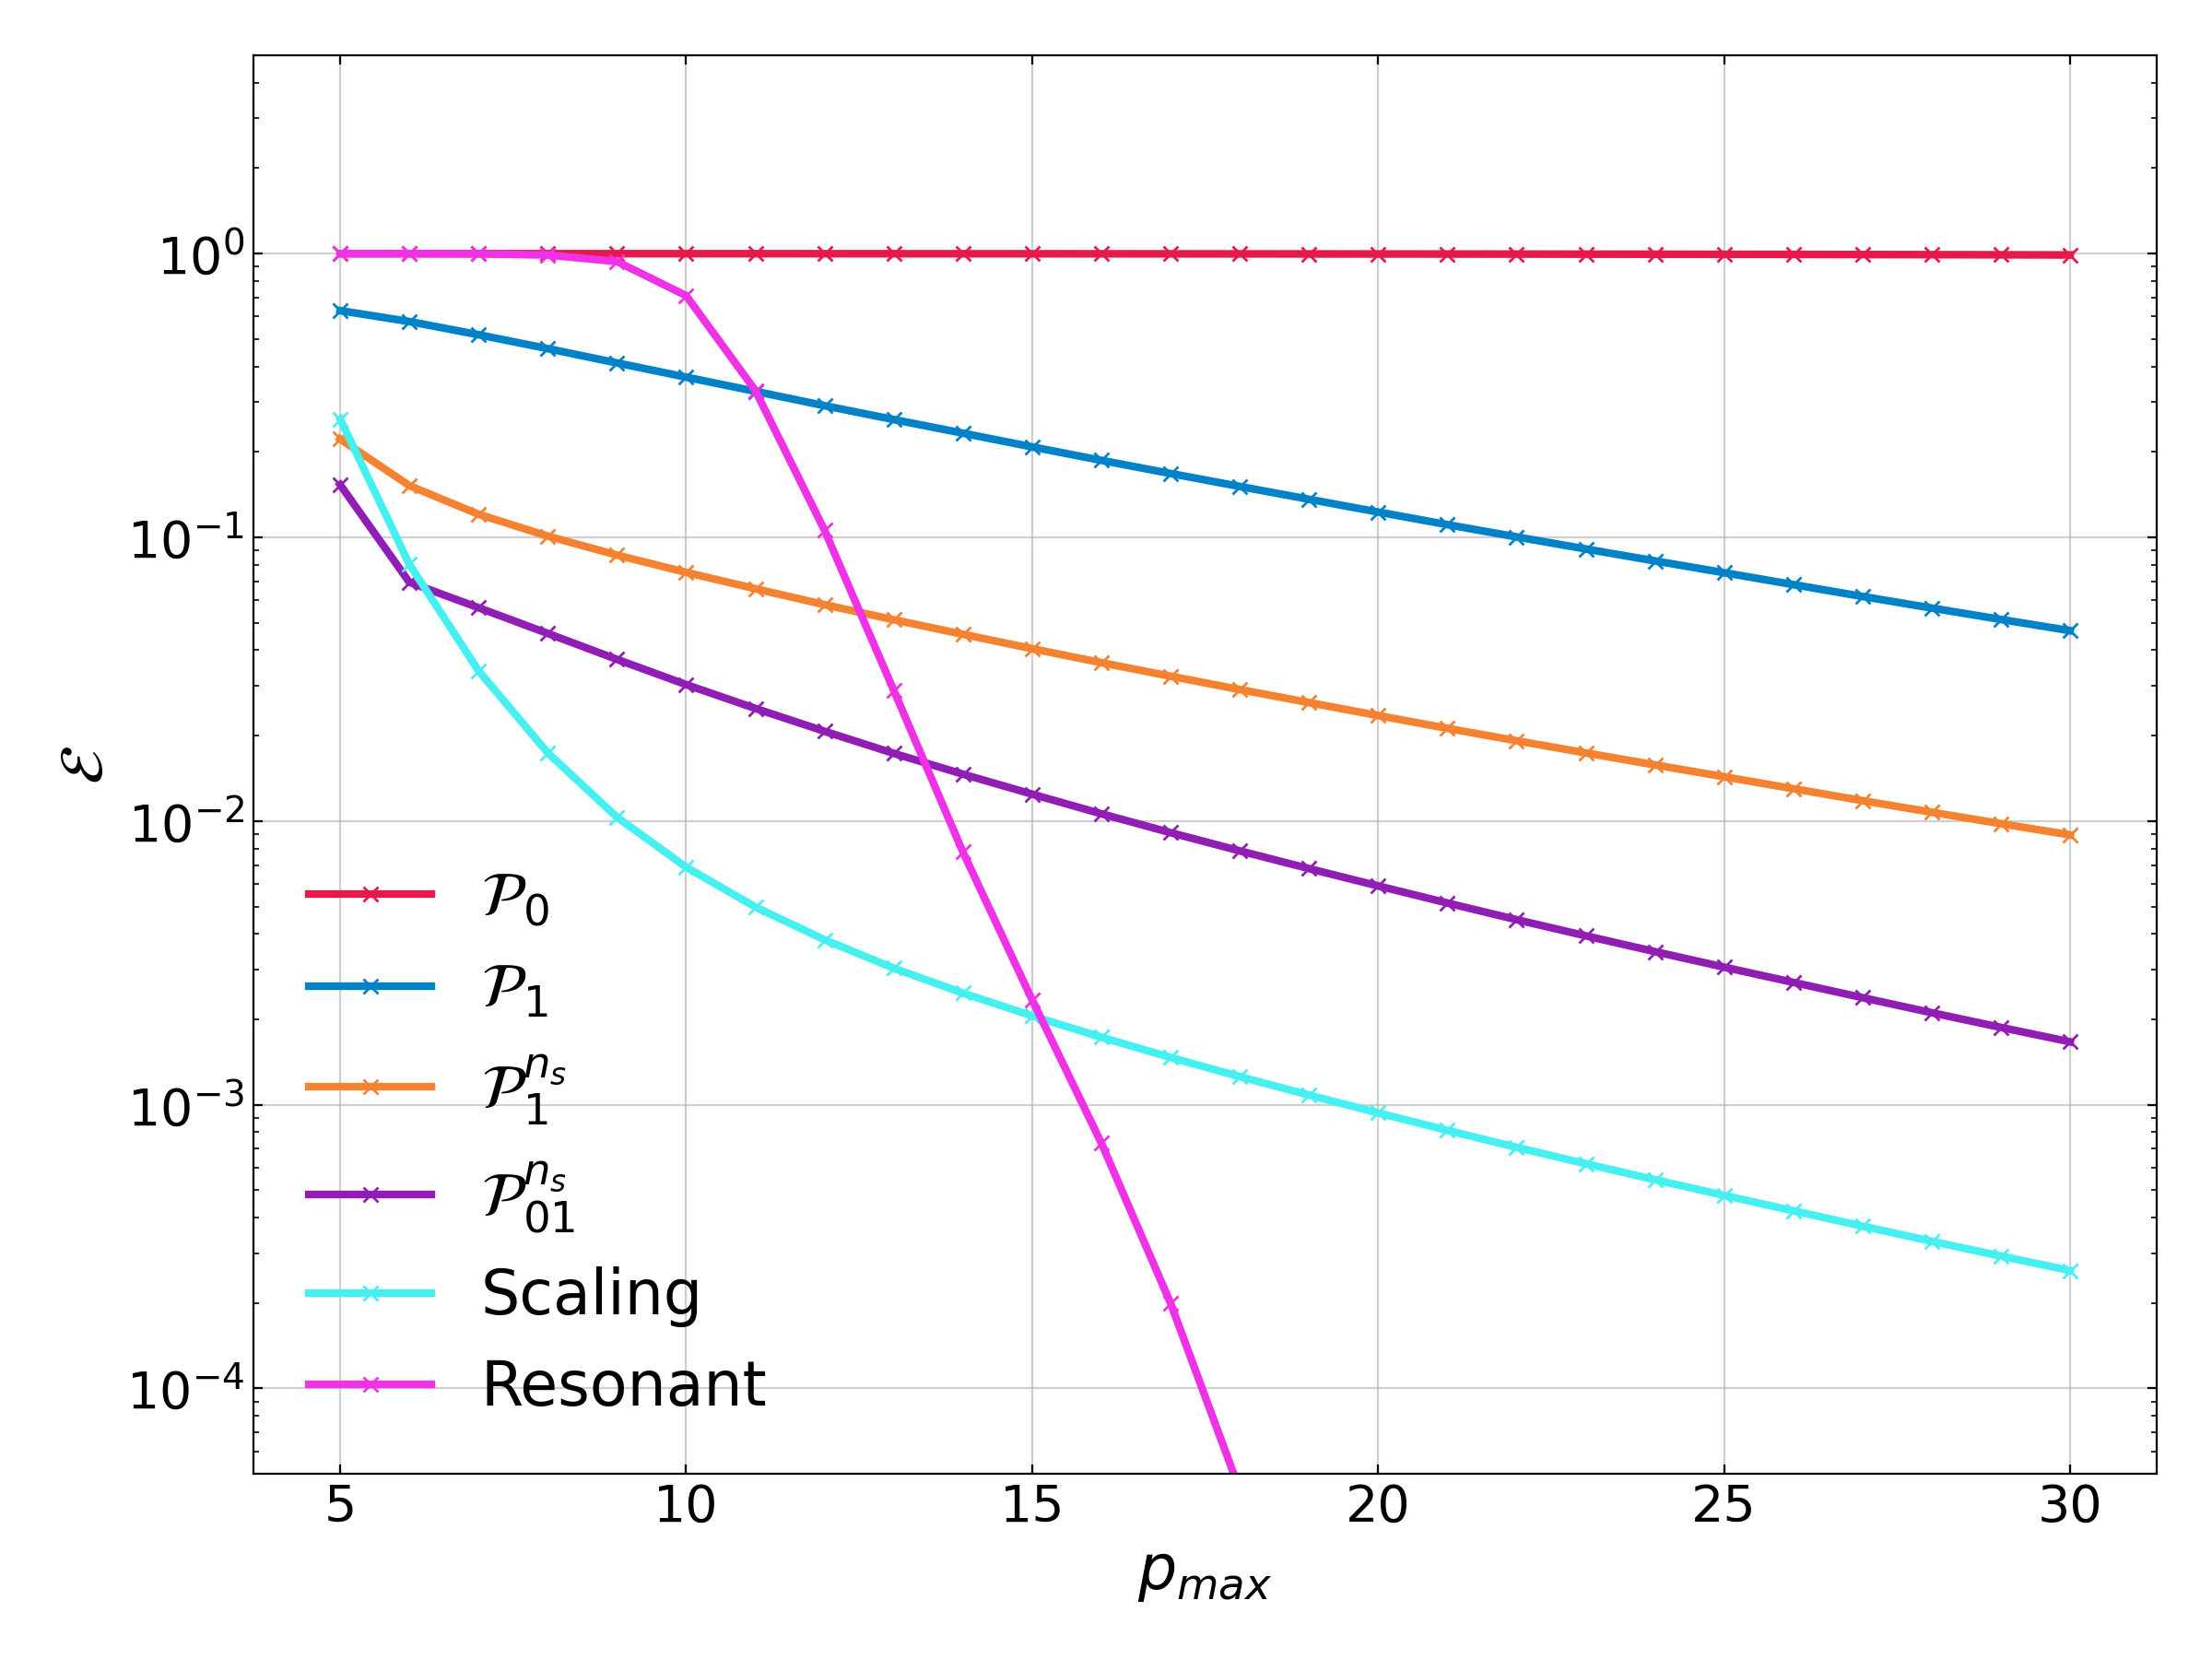
\includegraphics[width=.75\columnwidth]{pmax_reduction_plots_1_1000/dbi_scaling.png}}\\
\caption{
    For the scale-dependent DBI template~\eqref{dbi_prod_shape},
    by including a minimal amount of power spectrum information
    using~\eqref{Lns_inv} and~\eqref{Lns_both} ($\Lnsinv$ with
    $n_s^{*}=0.9649$), we can decrease the convergence error
    by nearly an order of magnitude (compared to $\Linvk$), reaching sub-percent errors at $\Pmax=30$.
    The $\scalingbasis$ basis performs far better again, even without the extra
    power spectrum information.
    By far the fastest convergence, however, results from the $\resobasis$ basis.
    The convergence of this template also has a dependence on $\kmax/\kmin$.
    The convergence power of these basis sets will allow us to efficiently
    capture the scale dependence of the numerically calculated shape function.
    }\label{fig:recon_dbi_ns}
\end{figure}

\begin{figure}[!pth]
\centering
\subfloat[$\cos(\omega(k_1+k_2+k_3))$]{\label{fig:freq_a}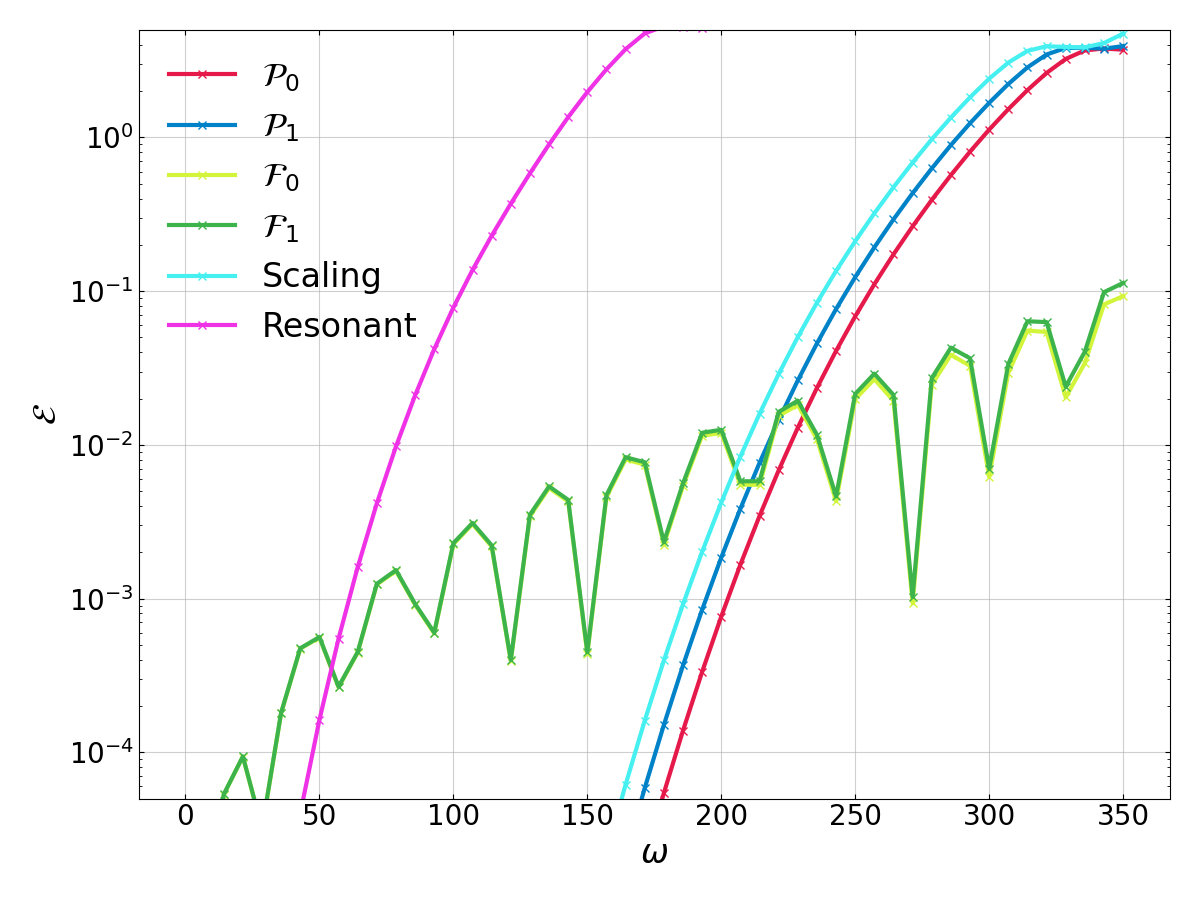
\includegraphics[width=.75\columnwidth]{freq_scan_plots/cos_freq_scan.png}}\\
\subfloat[$\cos(\omega\ln(k_1+k_2+k_3))$]{\label{fig:freq_b}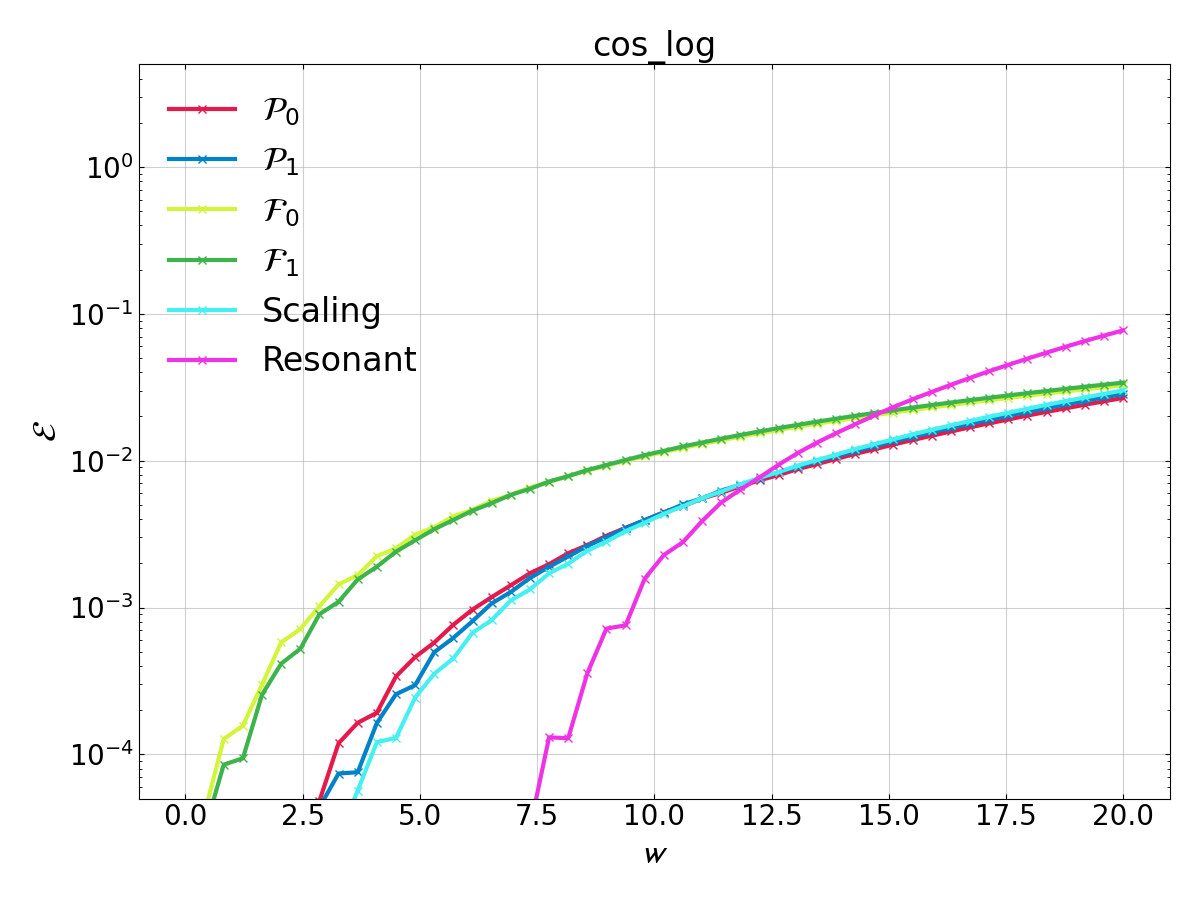
\includegraphics[width=.75\columnwidth]{freq_scan_plots/cos_log_freq_scan.png}}\\
\caption{
    Here we test our basis sets on oscillatory templates, which are a good proxy for feature models.
    These plots are useful to aid in deciding which basis to run $\cmbbest$ for,
    in determining which covers the widest range of features.
    The $\Lnsinv$ basis is not included in every plot, but would always perform between
    the $\Lbasic$ and $\scalingbasis$ basis.
    The basis sets are defined in Table~\ref{tab:basis_summary},
    and some are plotted in figures~\ref{fig:basis_pmax5_plots_a}
          and~\ref{fig:basis_pmax5_plots_b}.
    Basis sets~$\Linvk$ and $\scalingbasis$ work well for the linear oscillations,
    converging up to around $\omega\approx200$.
    For logarithmic oscillations the resonant basis works best, as expected.
    However, the improvement is less dramatic.
    }\label{fig:plot_freq_scan}
\end{figure}
\begin{figure}[!pth]
\centering
\subfloat[$\cos(\omega(k_1+k_2+k_3))S^{DBI}$]{\label{fig:freq_c}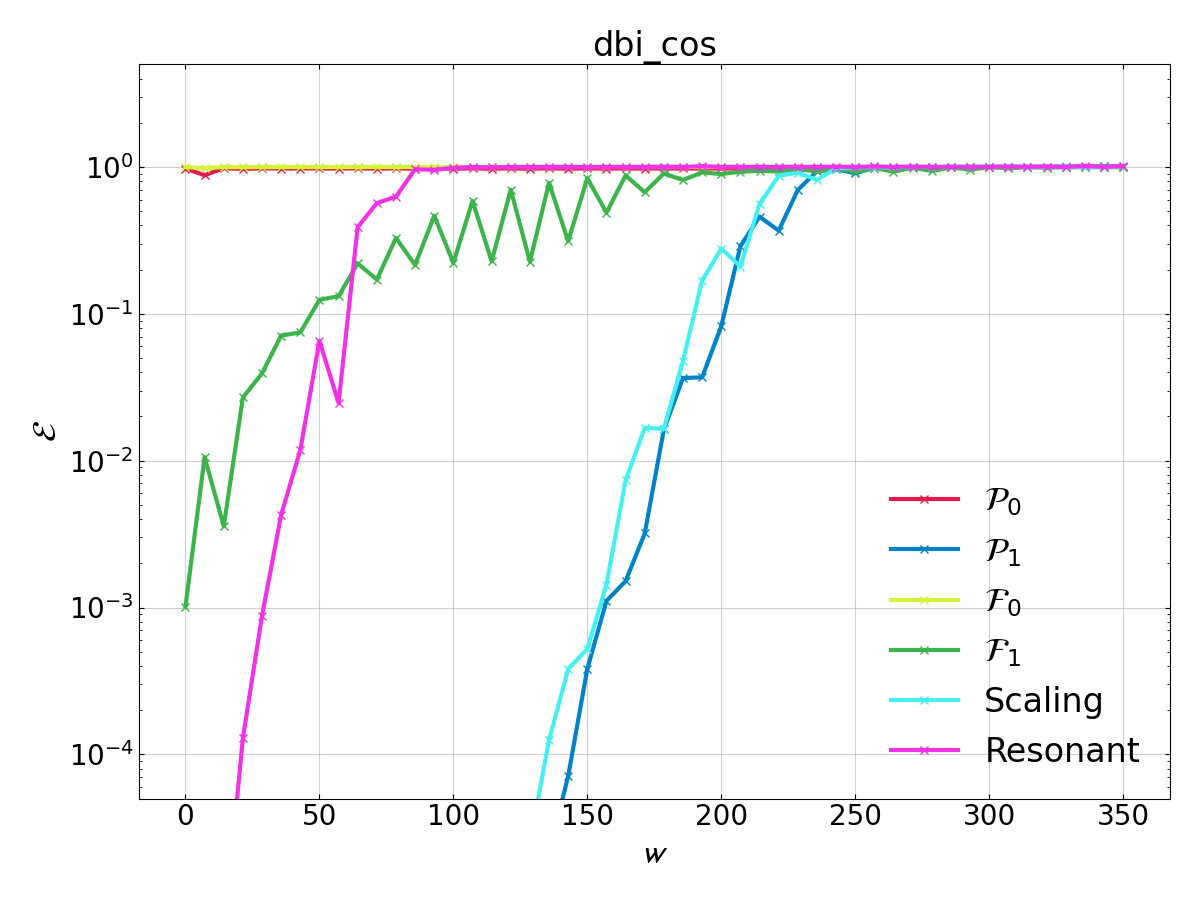
\includegraphics[width=.75\columnwidth]{freq_scan_plots/dbi_cos_freq_scan.png}}\\
\subfloat[$\cos(\omega\ln(k_1+k_2+k_3))S^{DBI}$]{\label{fig:freq_d}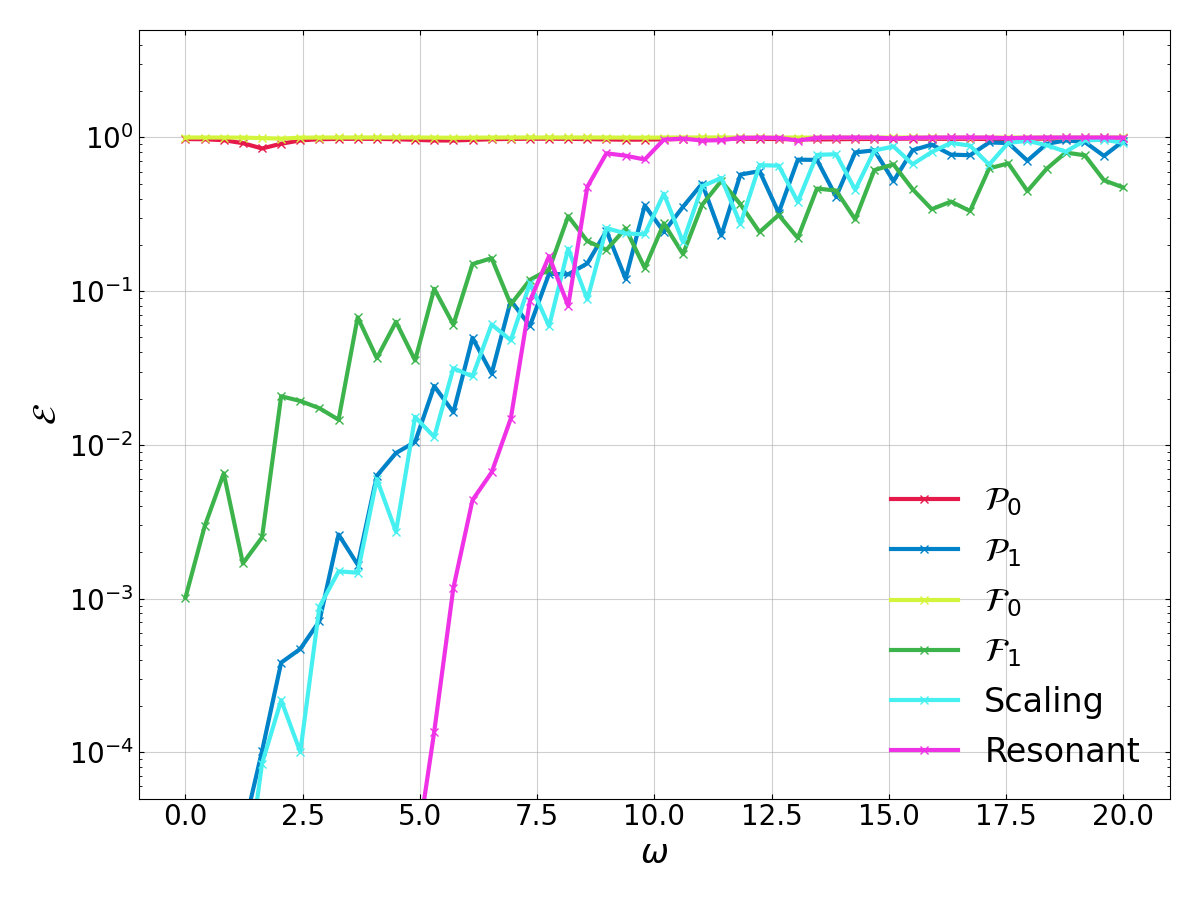
\includegraphics[width=.75\columnwidth]{freq_scan_plots/dbi_cos_log_freq_scan.png}}\\
\caption{
    We hold the basis size $\Pmax$ fixed at $30$ and increase the frequency of
    the oscillatory template.
    For linear oscillations with non-trivial shape dependence (a) we see that
    $\Lnsinv$ and the $\scalingbasis$ basis converge for a significantly larger
    frequency range than the $\resobasis$ basis, as expected.
    We also see that $\Fbasic$ and $\Finvk$ converge very poorly due to the
    DBI shape, only covering around a tenth of the frequency range that
    the $\scalingbasis$ basis converges for, up to $\omega\approx170$.
    For logarithmic oscillations the resonant basis converges best,
    capturing the complex oscillatory templates up to around $\omega\approx7$.
    Beyond this point none of the basis sets converge so the relative
    performance is irrelevant, but we can see that the $\resobasis$ basis
    actually has the largest error in this region---this is due to that basis
    being constructed out of orthogonal Legendre polynomials with
    a log-scaled argument.
    }\label{fig:plot_freq_scan_dbi}
\end{figure}

Finally, we consider convergence in the light of the more subtle scale-dependence due to
the spectral index $n_s$ of the power spectrum.
The simple canonical examples in Figure~\ref{fig:recon_malda_dbi} had shape dependence and no scale dependence,
but this would only be expected of scenarios unrealistically deep in the slow-roll limit.
When we include this scale dependence, using~\eqref{dbi_prod_shape} with $n^*_s$, 
it proves very useful to include these deviations from
integer power laws in the basis functions.  We will now consider two cases, first augmenting
$\Lbasic$ by a scale-dependent $1/k$ term using the orthogonalisation procedure~\eqref{gram_schmidt}, 
\begin{align}\label{Lns_inv}
    q_{\Pmax-1}(k) = \text{Orth}\left[{k^{-1+(n_s^{*}-1)}},~\Lbasic\right],
\end{align}
which we refer to as $\Lnsinv$.
Secondly, we instead augment $\Lbasic$ with an additional scale-dependent terms
\begin{align}\label{Lns_both}
    %q_{\Pmax}(k) = \text{Orth}\left[{k^{(n_s^{*}-1)}},~\Lbasic\right],\qquad  q_{\Pmax\text{$+$}1}(k) = \text{Orth}\left[{k^{-1+(n_s^{*}-1)}},~\Lbasic\right],
    {k^{(n_s^{*}-1)}},\qquad{k^{-1+(n_s^{*}-1)}}
\end{align}
which we refer to as $\Lnsboth$.


    It is worth noting that while $\Lbasic$ with (e.g.) $\Pmax=20$ is a subset of
    $\Lbasic$ with any higher $\Pmax$, $\Lnsinv$ with (e.g.) $\Pmax=20$ is not a subset of
    $\Lnsinv$ with any higher $\Pmax$ as the augmented term will be orthogonalised
    with respect to a different set of functions.


As we see in Figure~\ref{fig:recon_dbi_ns}, for equilateral type shapes
even a small overall scale dependence causes significant degradation in the convergence of
the original augmented Legendre basis $\Linvk$.
However, incorporating the spectral index $n_s$  into the basis functions $\Lnsinv$ and $\Lnsboth$
results again in rapid convergence to the scale-dependent DBI template, which can then be accurately
approximated with a limited number of modes.
We conclude using power spectrum information to augment the basis functions with terms incorporating the expected dependence
on the spectral index enables the efficient approximation of high precision primordial bispectra.
This is still not optimal, however, as the scaling of the bispectrum is not uniquely defined by the
scaling of the power spectrum, so more flexibility would be desirable---we will explore this further
in Section~\ref{sec:scaling_definition}.


\section{The $\scalingbasis$ basis}\label{sec:scaling_definition}
    Despite having the same power spectrum scaling,
    different models can have different bispectrum scalings.
    Therefore while the power spectrum can give us a
    rough estimate of the scaling of the bispectrum,
    the $\Lnsinv$ basis may not converge sufficiently quickly if~\eqref{Lns_inv}
    is not a sufficiently close match to the required scaling.
    We would instead like a basis that could fit
    a range of fractional powers of $k$.
    We achieve this using the $\scalingbasis$ basis.
    The $\scalingbasis$ basis is built using the Legendre polynomials,
    augmented (in the sense of~\eqref{gram_schmidt})
    with
    \begin{align}\label{scaling_basis_definition}
        k^{-1},\qquad \ln(k)k^{-1}
        %q_{\Pmax-2}(k) &= \text{Orth}\left[{k^{-1}},~\Lbasic\right],\\
        %q_{\Pmax-1}(k) &= \text{Orth}\left[{\ln(k)k^{-1}},~\Lbasic\right].
    \end{align}
    This is motivated by
    \begin{align}
        k^\epsilon &= e^{\epsilon\ln\left(\frac{k}{\kmin}\right)+\epsilon\ln(\kmin)}\\
                   &\approx e^{\epsilon\ln\left(\kmin\right)}
                      \left(1+\epsilon\ln\left(\frac{k}{\kmin}\right)\right)
    \end{align}
    which is valid when $\epsilon\ln\left(\kmax/\kmin\right)$ is
    sufficiently small.
    Since for the DBI case the scaling exponent $\epsilon$ is expected to be of the
    same order as $n_s-1$ and $\varepsilon_s$, we see that this
    approximation is good for our case,
    where (as we will discuss in Section~\ref{sec:tradeoff})
    we have $\ln\left(\frac{\kmax}{\kmin}\right)\approx6.91$.
    By adding $k^{-1}$ and $\ln(k)k^{-1}$ separately to our
    basis, their relative coefficient will be set to the value
    which provides the best fit to the final shape,
    providing the flexibility needed to fit shapes with different
    scalings with the same basis, so we have no need to know anything
    about the scaling a priori (except that it is small).


    For the feature templates, for example Figure~\ref{fig:plot_freq_scan},
    we see that the $\scalingbasis$ basis performs equivalently to $\Lnsinv$
    and $\Lbasic$.
    This is because these template have no simple power-law scaling or complex shape dependence,
    and the fit to the oscillatory feature is due to the Legendre polynomials
    in the basis.
    In Figure~\ref{fig:plot_freq_scan_dbi} we see that the $1/k$ behaviour is
    necessary to achieve an acceptable fit, but since these templates
    do not need non-integer scaling, the $\scalingbasis$ basis performs
    equivalently to $\Linvk$, as expected.


    As we can see in Figure~\ref{fig:recon_dbi_ns} however, the $\scalingbasis$ basis
    converges quickly to a DBI template with a realistic scaling. It outperforms
    the $\Lnsinv$ basis, despite not assuming power spectrum information.

\section{The $\resobasis$ basis}\label{sec:resobasis_definition}
    We finally describe a basis specifically designed to capture logarithmic oscillations,
    a type of feature that is usually very difficult to accurately fit.
    This goes against our philosophy of desiring a basis that is not tied to
    any specific shape, which was motivated by the fact that $\cmbbest$
    is expensive but need only be run once per basis.
    However, logarithmic oscillations are an important type of feature in the
    literature~\cite{Planck_NG_2018}.
    Running $\cmbbest$ twice, once for a basis that can cover
    a broad range of general features, and once for
    logarithmic oscillations in particular,
    may be a viable strategy to cover a very broad range of models.


    The $\resobasis$ basis is built using the Legendre polynomials,
    however the argument has been scaled logarithmically.
    It differs from the basis described in~\cite{Funakoshi} in that it
    also includes a factor of $\frac{1}{\sqrt{k}}$ to retain orthogonality.
    We define the $n$th basis element as
    \begin{align}\label{reso_basis_definition}
        \frac{P_n(\bar{k})}{\sqrt{k}}\text{,}\qquad \bar{k}=\frac{2\ln(k)-\ln(\kmin\kmax)}{\ln(\kmax)-\ln(\kmin)}.
    \end{align}
    We then see that
    \begin{align}
        \int_{\kmin}^{\kmax}dk\frac{P_m(\bar{k})}{\sqrt{k}}\frac{P_n(\bar{k})}{\sqrt{k}}
        = \int_{\ln\kmin}^{\ln\kmax}d\ln{k}~P_m(\bar{k})P_n(\bar{k})
        \propto \delta_{mn}
    \end{align}
    so the $\resobasis$ basis is orthogonal
    due to the way we defined $\bar{k}$ for this basis set.

    In Figure~\ref{fig:plot_freq_scan} we see that for linear oscillations, as expected,
    the $\resobasis$ basis converges for a much smaller range for frequencies
    (for fixed basis set size $\Pmax=30$) than the other basis sets we test.
    For logarithmic oscillations however, we see that the range of accessible
    frequencies is nearly doubled when compared to the other basis sets.
    We also note that for logarithmic oscillations,
    wherever we have acceptable convergence the $\resobasis$ basis converges best.
    We also see however that in the frequency range where none of our basis sets
    converge, the $\resobasis$ basis has the largest error. This is because
    the $\resobasis$ basis is designed to be a set of orthogonal logarithmic
    oscillations, and so will be orthogonal to frequencies outside of its range.
    On the other hand, while the $\scalingbasis$ basis (for example) has
    a worse fit for lower frequencies, it has a better fit to higher frequencies as
    it is not orthogonal to them. We emphasise however that this only occurs
    in the region where none of our basis sets provide acceptable convergence
    for $\Pmax=30$.

    We also note the surprising result in Figure~\ref{fig:recon_dbi_ns}
    that the $\resobasis$ basis performs best at converging to the
    scale-dependent DBI template. However, the convergence of the
    $\scalingbasis$ basis is still perfectly adequate in this case.
    \begin{figure}[!pth]
        \centering
        \subfloat[$\Lbasic$]{\label{fig:basis_plot_a}\includegraphics[width=.85\columnwidth]{basis_plot_diagrams/basis_pmax5_plot_P_0}}\\
        \subfloat[$\Linvk$]{\label{fig:basis_plot_b}\includegraphics[width=.85\columnwidth]{basis_plot_diagrams/basis_pmax5_plot_P_1}}\\
        \subfloat[$\scalingbasis$ basis]{\label{fig:basis_plot_e}\includegraphics[width=.85\columnwidth]{basis_plot_diagrams/basis_pmax5_plot_scaling}}\\
        \caption{
            We plot the $\Lbasic$, $\Linvk$ and $\scalingbasis$ basis sets from
            Table~\ref{tab:basis_summary}, for $\Pmax=5$. Note that these sets
            have Legendre polynomial basis elements in common, but differ in
            which functions they are augmented by, which are added to the start of the
            indexing.
        }\label{fig:basis_pmax5_plots_a}
    \end{figure}
    \begin{figure}[!pth]
        %\ContinuedFloat
        \centering
        \subfloat[$\Fbasic$]{\label{fig:basis_plot_c}\includegraphics[width=.85\columnwidth]{basis_plot_diagrams/basis_pmax5_plot_F_0}}\\
        \subfloat[$\Finvk$]{\label{fig:basis_plot_d}\includegraphics[width=.85\columnwidth]{basis_plot_diagrams/basis_pmax5_plot_F_1}}\\
        \subfloat[$\resobasis$ basis]{\label{fig:basis_plot_f}\includegraphics[width=.85\columnwidth]{basis_plot_diagrams/basis_pmax5_plot_reso}}\\
        \caption{
            We plot the $\Fbasic$, $\Finvk$ and $\resobasis$ basis sets from
            Table~\ref{tab:basis_summary}, for $\Pmax=5$. Note that
            $\Fbasic$ and $\Finvk$
            have Fourier basis elements in common, but differ in
            which functions they are augmented by. The $\resobasis$ basis
            differs in all of its basis elements, lacking even
            a constant basis element due to the factor of
            $1/\sqrt{k}$ added to retain orthogonality.
        }\label{fig:basis_pmax5_plots_b}
    \end{figure}


\section{Large non-physical contributions}\label{large_non_physical}
    When a shape is dominated by its non-physical configurations
    (those that do not obey the triangle inequality~\eqref{triangle_inequality})
    then we can see slow convergence on the tetrapyd, despite
    possibly fast convergence on the cube as a whole.
    We will refer to convergence on the tetrapyd as $\totalcortet$
    and the convergence on the cube as $\totalcorcub$.
    For a pure oscillation we see no significant difference between the convergence on the cube
    and on the tetrapyd, as expected for a shape where the physical and non-physical
    configurations are of the same order of magnitude.
    For an oscillation with a DBI shape however, we see a large difference,
    as shown in Figure~\ref{fig:log_recon_osc_dbiosc}.
    On the cube we see fast, monotonic convergence---the $\resobasis$ basis
    and $\scalingbasis$ basis perform well, quickly bringing $\totalcorcub$
    below $0.1\%$.
    On the tetrapyd however, we see that $\totalcortet$ only drops below
    $0.1\%$ for $\Pmax<30$ for the $\resobasis$ basis.


    We also see that the improvement in $\totalcortet$ is no longer
    monotonic, there are regions where increasing $\Pmax$ results in
    a larger $\totalcortet$.
    To understand this it is important to remember that we are not simply
    adding modes as we increase $\Pmax$---the augmented mode is changing
    each time, and thus while we expect $\totalcorcub$ to decrease monotonically,
    there is no such guarantee for point-wise convergence.


    We also notice that $\totalcortet$ stays fixed at $1$ for low values of $\Pmax$.
    This is due to the basis fitting the large non-physical configurations,
    and thus in~\eqref{relative_difference}, $S_2 \gg S_1$ everywhere on the tetrapyd.
    \textcolor{red}{Double check.}


    For the local shape the mean value of the shape function on the entire cube
    (thus accounting for volume effects) is approximately a factor of $40$ larger than the mean
    when restricted to the tetrapyd. For the equilateral template, this factor becomes $-300$.
    This illustrates why the tetrapyd-vs-cube problem is so much more severe for equilateral-type
    shapes than for local shapes, as the non-physical configurations are an order of magnitude
    more dominant.


    This phenomenon is a major obstacle to preserving the separability of the in-in formalism,
    due to the restriction that we must (effectively, if not in a literal sense) fit to the cube---we
    have seen that neglecting it and using a simple basis such as $\Lbasic$ would be disastrous.
    However, as we have seen, the more sophisticated basis sets described in this chapter are capable
    of overcoming this obstacle, without surrendering generality.

\section{A tradeoff between $\Pmax$ and $\kmax/\kmin$}\label{sec:tradeoff}
    While it may not be intuitively apparent, the value of $\kmax/\kmin$
    affects convergence even in the absence of significant features.
    We can see this in Figure~\ref{fig:recon_dbi_ns}.
    In this figure we plot the convergence of various basis sets for the scale-dependent
    DBI template~\eqref{dbi_prod_shape}, for $\kmax/\kmin=550$ and
    for $\kmax/\kmin=1000$. We see that the convergence is slower
    for higher $\kmax/\kmin$. This means that to achieve the same convergence
    for this shape for a higher $\kmax/\kmin$, we must also go to a higher $\Pmax$.
    For example, if one wanted to achieve an accuracy of $0.1\%$ for this shape
    with the $\scalingbasis$ basis,
    one would need $\Pmax=15$ for $\kmax/\kmin=550$
    and $\Pmax=20$ for $\kmax/\kmin=1000$.
    We also see this effect for the scale-invariant DBI shape~\eqref{dbi_shape}
    but it is significantly less dramatic.


    We of course desire to use as much of the available data as we can.
    As such, it is desirable to have the largest possible $k$-range.
    However, as we can see, this must be weighted against the loss
    of descriptive power, as we will then have a smaller set of shapes which
    will converge sufficiently well to be constrained.


    As described in~\cite{Sohn_2021}, if too much of the squeezed limit is lost,
    constraining power on models such as those of the local type is lost (at the $\cmb$ level).
    It is shown in that work that $\kmax/\kmin=1000$ is sufficient, and as we have seen in this chapter
    this value still retains convergence on a range of interesting models at the primordial level.


%\section{Factor basis?}
%    Words~\cite{tensor_decomp_review}.
%\section{Higher $\Pmax$}
%    Going beyond $\Pmax=30$.
%    How high can I go, in terms of parameters that can't be compared to Planck?
\section{Conclusions}
    From the plots presented in this chapter it is clear that the problem of the
    large non-physical off-tetrapyd configurations is vitally important to the feasibility of the
    separable in-in calculation of inflationary bispectra.
    In this setting, where we are effectively forced to fit on the whole cube,
    we find that the basic Legendre polynomials or Fourier series basis sets alone
    are not sufficient to capture the shapes we hope to constrain.
    However, we found that by augmenting the Legendre polynomials with
    basis functions that could capture $1/k$ behaviour, the convergence
    increased dramatically and the range of shapes that could be constrained by
    this pipeline broadens significantly.


    Our basis sets and their definitions are summarised in Table~\ref{tab:basis_summary},
    and a selection are plotted in Figures~\ref{fig:basis_pmax5_plots_a}
    and~\ref{fig:basis_pmax5_plots_b}.
    While $\Lnsinv$ improves significantly over $\Lbasic$ for certain examples,
    as it is tied to a particular scaling it is not an ideal solution. This is due to the desire to create
    a full pipeline, which connects to real $\cmb$ data using $\cmbbest$, and the constraint
    that the expense of that code (for reasonably large $\Pmax$) limits the full pipeline to one (or very few) basis sets.
    Thus we desire a single basis that can capture the broadest range of shapes, including different scalings.
    To improve upon $\Lnsinv$, we introduced the $\scalingbasis$ basis, which is augmented by
    terms which allow it more flexibility in capturing the scaling of the shape function,
    despite being built without any power spectrum information.


    We also presented results from the $\resobasis$ basis, a basis set designed to converge well
    for logarithmic oscillations, an important target due to the resonance mechanism.
    While this goes against the philosophy of developing one basis set that converges well across the
    broadest possible range of bispectrum shapes, it may be useful as an alternative way forward---performing
    two runs of $\cmbbest$, i.e.\ with both the scaling basis (for linear oscillations and general features)
    and the resonant basis (for logarithmic oscillations).


    Possible future improvements in the design of basis sets could be obtained using tensor decomposition methods,
    such as the \textsc{parafac} method described in, for example,~\cite{tensor_decomp_review}.
    Given the output of $\primodal$,
    the coefficients $\alpha_{pqr}$, one could imagine performing a tensor decomposition on $\alpha_{pqr}$,
    approximating it as a sum of outer products of vectors.
    If this decomposition resulted in a compact description, a sum of only a few terms, then it is possible
    the methods of $\cmbbest$ as described in~\cite{Sohn_2021} could be efficiently applied to individual
    models, as this would effectively have a much smaller $\Pmax$. This could allow a very broad,
    but still template-free, analysis of bispectrum constraints on inflationary models.


    Now that we have demonstrated the feasibility of the overall method, in the next chapter we will
    present its detailed implementation in the context of the in-in formalism.





\chapter{Methods and Validation}\label{chapter:methods}
\section{Numerics of mode evolution}
    \subsection{Choice of time coordinate}
    $\tau_s$
    \subsection{The initial conditions}
    When to set IC's for each mode.
    \subsection{Factoring out oscillatory behaviour}
    Swapping variables.
    \subsection{Freeze-out}
    Words
\section{Integration methods}
    \subsection{The $i\varepsilon$ prescription}
    Words
    \subsection{Contrast with previous work}
    Words
    \subsection{Suppression at early times}
    Intuition for suppression from plane wave expansion.
\section{Starting the integration with a pinch}
(Contrast this to $i\varepsilon$!!)
The previous two sections detailed the methods required to calculate
the coefficients $\alpha_n$ in~\eqref{goal}, obtaining an
explicitly separable expression for the shape function.
In this set-up,
there are two kinds of integrals we must compute: integrals over time of
the form~\eqref{inin_kindep}, and integrals over $k$ of the form~\eqref{mode1Dcoeffs_integral}.
The first is done once per coefficient for each vertex, the second is a decomposition
done once for $\zeta_k$ and $\zeta_k'$ each, every timestep.
In this section we detail how to numerically evaluate these
integrals accurately and efficiently.


Since calculating each point in the time integrand requires a
decomposition~\eqref{mode1Dcoeffs_integral}, which is highly oscillatory
at early times, it is worthwhile to consider how to perform the
time integral efficiently. From the form of the Bunch-Davies mode functions,
we expect the dominant frequency (in $\tau_s$) to be $3\kmax$.
Assuming we are earlier than any features that might change this,
we can use this knowledge to sample the integrand at a far lower rate,
building the oscillation into our quadrature weights.
A second important consideration comes from how early we sample the integrand.
We can of course only obtain a point in the time integrand after our mode
functions have burned in from their set initial conditions to their true
attractor trajectory. This means that sampling earlier in the time integrand
requires us to set the initial conditions for the mode functions deeper
in the horizon, a regime in which they are expensive to evolve.


The integrals of the form~\eqref{inin_kindep} that we must calculate have $\tau=-\infty$ as their lower limit.
The highly oscillatory nature of the mode functions in these early times ($\lvert k\tau_s\rvert\gg1$) suppresses the
coefficients of our basis expansion by a factor of $1/\tau_s$.
As noted in~\cite{Funakoshi}, this means that we do not need to
explicitly use the $i\varepsilon$ prescription to force the integrals to converge.
In the case of using the Legendre polynomials as our
basis, we can see this more precisely by considering
the plane wave expansion (e.g.~\cite{finite_ft_legendre}):
\begin{align}\label{exp_expansion}
    e^{-i\bar{k}(\kmax-\kmin)\tau/2} = \sum_{n=0}^{\infty}(2n+1)i^n P_n(\bar{k})j_n(-(\kmax-\kmin)\tau/2)
\end{align}
for $\bar{k}$ in $[-1,1]$. When $(\kmax-\kmin)\tau/2$ is large, the spherical Bessel functions
oscillate with an amplitude $\propto\frac{1}{\tau}$. Thus,
the initial conditions~\eqref{bd_ic} expanded in Legendre polynomials (and similar)
give us suppression of $1/\tau^3$ in~\eqref{inin_kindep}.


While our method has extra suppression compared to configuration-by-configuration methods
(and thus does not need the $i\varepsilon$ prescription to converge)
it still converges rather slowly, as we push the lower limit to earlier times.
This expensive sampling can be wasteful of resources,
especially in a feature scenario where we know this
region will not contribute to the final result.
Care is required however, as starting the integration in the wrong way can easily lead to
errors which can completely swamp the result, since higher order modes
are more sensitive to early times.
The authors of~\cite{chen_easther_lim_1} used an artificial damping term to smoothly
``turn on'' their integrand.
The point at which this is done can then be pushed earlier to check for convergence.
However they found that the details of the damping needed to
be carefully set to avoid underestimating the result.
In~\cite{chen_easther_lim_2} they replaced this method by a ``boundary regulator'';
they split the integral into early and late parts and used integration by parts to
efficiently evaluate the early time contribution.
As our integrand already has extra suppression compared to the configuration-by-configuration
integrands considered in~\cite{chen_easther_lim_1,chen_easther_lim_2},
we can safely use the simpler first method.


We understand this situation by
taking advantage of asymptotic behaviour of highly oscillatory
integrals (for a review see~\cite{iserles_2005}).
Since the leading order term depends on
the value of the non-oscillatory part only at the endpoints,
and the next-to-leading order correction depends on the
derivative only at the endpoints, we can approximate the integral
$\int_{-\infty}^T f(\tau_s)e^{iw\tau_s}d\tau_s$
by replacing the non-oscillatory part $f(\tau_s)$ with a function with
matching value and derivative at $\tau_s=T$,
but which converges far faster.
We use
\begin{align}\label{smooth_cutoff}
f(\tau_s)e^{-\beta^2(\tau_s-T)^2},
\end{align}
for $\tau_s<T$.
In this way, for sufficiently large $T$,
we obtain the accuracy of the
first two terms of the asymptotic expansion
($O(\beta^2/w^2)$, $w=3\kmax$) without needing to explicitly
calculate the derivative at $T$, or needing any phase information (as
one would need to accurately impose a sharp cut on the integrand).


\begin{figure}[!pth]
\centering
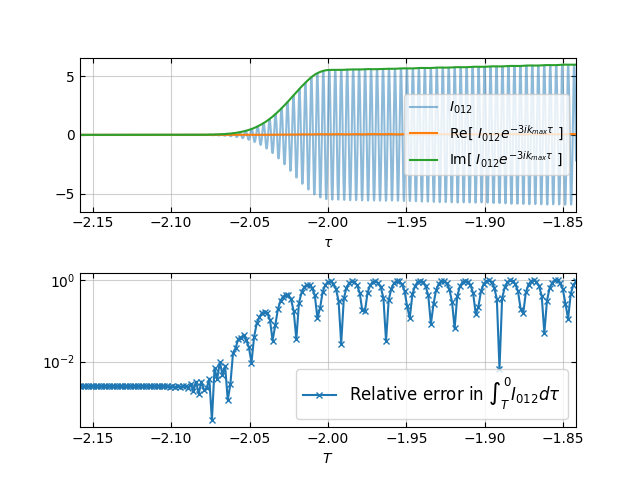
\includegraphics[width=\columnwidth]{plots/time_integrand.png}
\caption{
    A toy example demonstrating the considerations involved in performing the
    time integrals~\eqref{inin_kindep}.
    By carefully starting the time integrations,
    using the form~\eqref{smooth_cutoff}, we can avoid
    errors that would otherwise swamp our result.
    The coefficient being calculated is the
    $\alpha_{012}$ coefficient of the $\Lbasic$ expansion of~\eqref{example_eft2}.
}\label{fig:time_integrands}
\end{figure}

\begin{figure}[!pth]
\centering
    \subfloat[$\mathcal{E}$ for DBI model.]{\label{fig:a}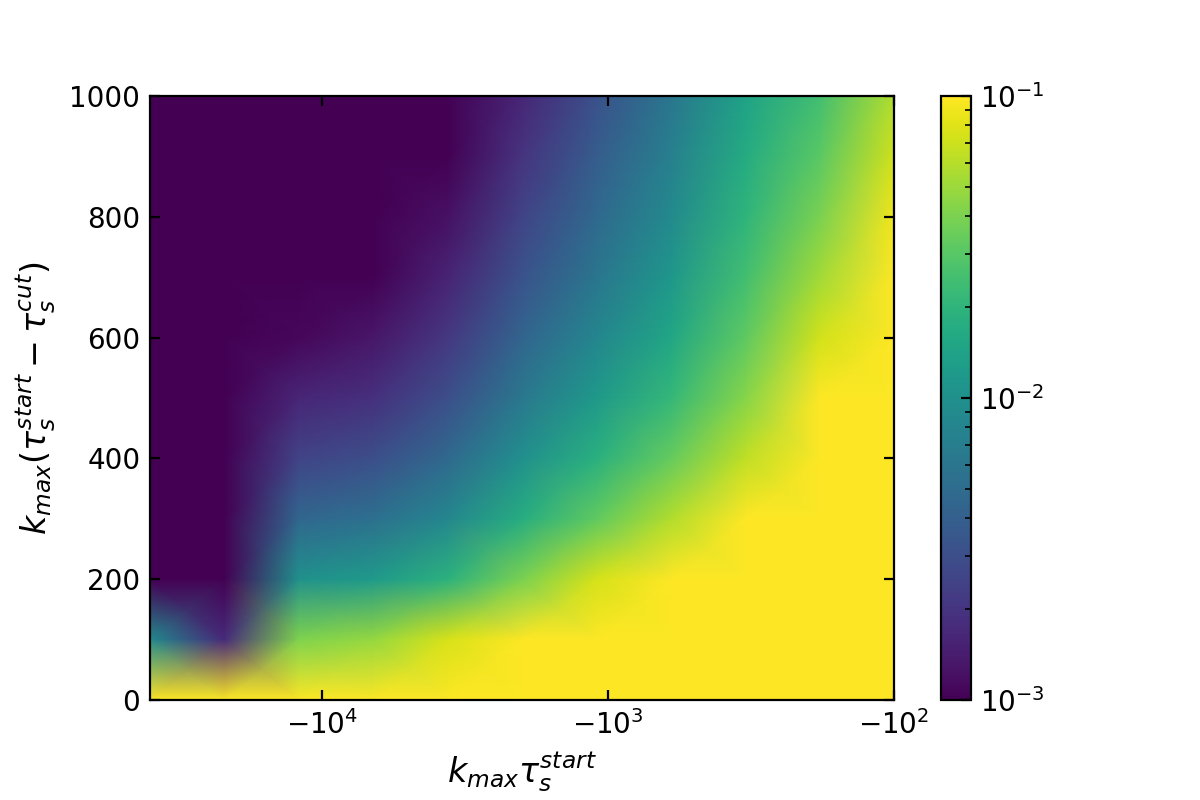
\includegraphics[width=.75\columnwidth]{time_integrand_convergence_plots/time_integrand_convergence_dbi.png}}\\
    \subfloat[$\mathcal{E}$ for resonant model.]{\label{fig:b}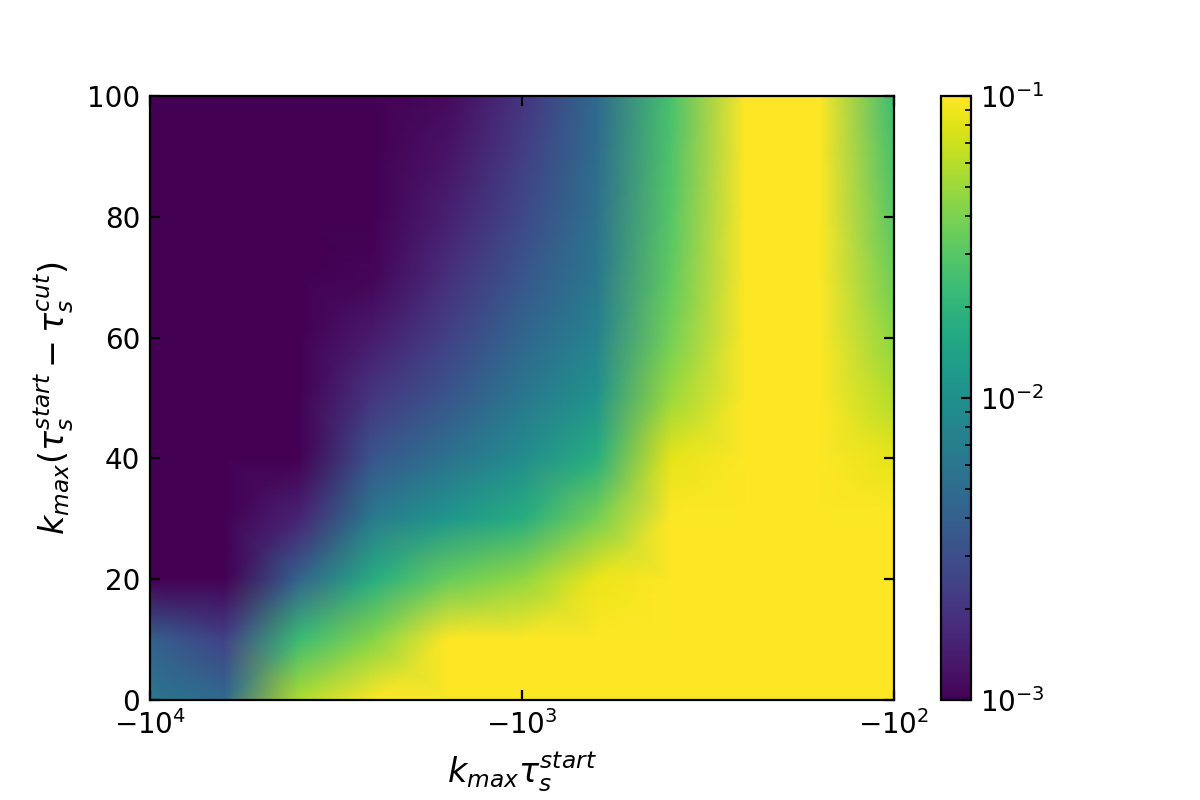
\includegraphics[width=.75\columnwidth]{time_integrand_convergence_plots/time_integrand_convergence_malda_reso_0.02.png}}\\
\caption{
    Here we show the convergence in $\tau_s^{start}$ and $\tau_s^{cut}$ for a DBI scenario and a resonant scenario
    (with a canonical kinetic term, on a quadratic potential).
    Note the different scales on the top and bottom plots.
    We quantify the convergence by plotting the error compared to the fully converged result,
    measured by $\mathcal{E}$.
    In both cases, the error is unacceptably high for a sharp cut, $\tau_s^{start}-\tau_s^{cut}=0$,
    across the entire width of the scan. However, for even moderately positive values of $\tau_s^{start}-\tau_s^{cut}$
    we see that the error can be reduced by orders of magnitude, for the same computational cost
    (i.e.\ the same $\tau_s^{cut}$).
    In both cases we also see that for values of $\tau_s^{start}$ which are too late in time,
    we do not recover the correct result in the range of the scan. This is expected,
    as in this case we are losing relevant physical information.
    }\label{fig:plot_time_integrand_scan}
\end{figure}


We use a damping of the form $e^{-\beta^2{(\tau_s-T)}^2}$ for $\tau_s<T$ to smoothly
set the integrand to zero before a certain initial time, $T$.
As long as $T$ is sufficiently early and $\beta$ is not too large
their precise values have no significant effect on the final result.
For definiteness, we take $\beta/w=1\times10^{-4}$, small enough that
the integrand has many oscillations while it is ``turning on'',
so matches the contribution of an infinite limit to high accuracy.
We demonstrate this in figure~\ref{fig:time_integrands}
for a toy $\Hint=(-1/\tau)\dot{\zeta}^3$,
as in~\eqref{example_eft2}.


We also demonstrate this for a realistic DBI model and resonance model
in figure~\ref{fig:plot_time_integrand_scan}.
Here we reparametrise the damping in a form that with a more obvious physical
interpretation.
We use the form $e^{-100{\left(\frac{{\tau_s^{start}-\tau_s}}{\tau_s^{start}-\tau_s^{cut}}\right)}^2}$.
The point $\tau_s=\tau_s^{start}$ is the earliest point we calculate the integrand for,
i.e.\ before this point we set the integrand to exactly zero---we
see that at this point the integrand is suppressed by a factor of $e^{-100}$.
In figure~\ref{fig:plot_time_integrand_scan} we see that $\tau_s^{start}-\tau_s^{cut}=0$
gives unacceptably large errors across the range of the scan, but for sufficiently large
$\tau_s^{start}$ this is ameliorated by a positive $\tau_s^{start}-\tau_s^{cut}$.
This effect is more relevant for the DBI scenario, as the size of the errors coming
from early times can easily dominate the final result, whereas in the resonant example
the large contributions from the resonance at later times is more robust.
For the resonant scenario~\eqref{eq:resonant_potential} we have $c_s=1$,
so we expect (from~\cite{flauger_pajer_resonant}) the point of resonance $\tau^k_s$
for each mode $k$ to be approximately given by $\tau^k_s = \frac{-\left|\phi'\right|}{2fk}$.
For our example, we have $\phi'\approx-0.14$, $f=0.02$, $\kmin=2.088\times10^{-4}$ and $\kmax=2.088\times10^{-1}$.
This means that we expect the earliest physically relevant time to be
$\tau_s\approx-\frac{0.14}{2(0.02)(2.088\times10^{-4})}\approx-1.7\times10^{4}$.
Indeed, in figure~\ref{fig:plot_time_integrand_scan} we see that $\kmax\tau_s^{start}$ must be
set earlier that $-10^3$ to correctly capture the feature.
\textcolor{red}{CHECK THIS.}


To obtain a $k$-sample we must evolve a Fourier mode from Bunch-Davies initial conditions deep in the horizon
until it becomes constant after horizon crossing.
We denote by $N_k$ the number of Fourier modes we evolve.
Different choices of distributing the k-samples are possible; for example, one could distribute them
with an even spacing, log-spacing or cluster them more densely near $\kmin$ and $\kmax$.
The $k$-integrals themselves can be computed quite efficiently since
at every timestep the integral is over the same sample points.
One can therefore calculate and store the values of the basis functions at each of these points,
along with the integration weights which will depend on the distribution of $k$-samples.
The actual integration at each timestep, the calculation of the 
coefficients in~\eqref{mode1Dcoeffs_integral}, then becomes nothing more
than a dot product of a time-independent array with the
numerically evolved mode functions, for each order up to $\Pmax$.
We have found the best convergence results from distributing the k-samples
according to the prescription of Gauss-Legendre quadrature.


To calculate the basis expansion of the bispectrum using the in-in formalism
we must first calculate the basis expansion of the mode
functions at each timestep~\eqref{mode1Dcoeffs_integral}.
At early times the mode functions are highly oscillatory, taking the form $z_k e^{-ik\tau_s}$
for some much smoother $z_k$.
Directly decomposing this would require evolving more $\zeta_k$ samples
than is practical.
We want an expansion of the form
\begin{align}\label{mode_expansion}
	z_k e^{-ik\tau_s} = \sum_{n=0}^{\infty}\alpha_n q_n(k).
\end{align}
We can obtain this by using standard oscillatory
quadrature, if the $\tau_s$ dependence of the weights does not add too much overhead.
We can also use an expansion of $e^{-ik\tau_s}$
with a known explicit time dependence, for example
the expansion~\eqref{exp_expansion}.


To use this second method,
the first (smooth) factor $z_k$ can be expanded in whatever basis we are working in, $q_n(k)$,
and the second factor (highly oscillatory in $k$) is expanded
in some convenient basis $\tilde{q}_n(k)$
(e.g.\ $\Fbasic$, or $\Lbasic$ using the analytic form~\eqref{exp_expansion}).
Then by precomputing
$q_a(k)\tilde{q}_b(k)$
as a linear combination of the set of basis functions $q_c(k)$
all we need calculate at each timestep is the coefficients
of the smoother $z_k(\tau_s)$, which we then convert to the coefficients
of $F^{(i)}(\tau, k)$. In this way we can retain flexibility in our
bispectrum basis, as well as efficiency and precision in the calculation.
In the case of using $\Lbasic$ for the $\tilde{q}_n(k)$,
assuming the expansion in~\eqref{shapemodeexp} converges,
we need only compute the expansion for $e^{-ik\tau_s}$ to enough
terms that the first $\Pmax$ of the
coefficients in the expansion~\eqref{mode1Dcoeffs_sum} of the $F^{(i)}(\tau, k)$ converge,
not until the actual sum~\eqref{mode1Dcoeffs_sum} converges, since for high enough orders the integrals
in~\eqref{inin_kindep} will integrate to zero.


Clearly, once $\tau_s$ becomes small enough these considerations will no longer be necessary
and we can simply decompose the mode function directly.
We do this around the horizon crossing of the geometric mean of $\kmin$ and $\kmax$.
If there is an extreme feature which causes a large deviation from the usual slow-roll form
this switch will need to be made sooner. 
Also, this method would need to be adapted for non-Bunch-Davies initial conditions.
Since anything related to the basis but independent of the scenario can be
precomputed, certain parts of this calculation do not hurt the efficiency of this
method in the context of, for example, a parameter scan.
Using the methods outlined above,~\eqref{inin_kindep} and~\eqref{mode1Dcoeffs_integral}
can be computed precisely and efficiently in a mostly basis-agnostic context
allowing us to ({\romannumeral 1}) preserve the intrinsic separability of the tree-level
in-in formalism and ({\romannumeral 2}) do so in a way that allows easy exploration of possible
sets of basis functions, to find a set that converges quickly enough to
be useful in comparison with observation.
    \subsection{When to start the integration}
    Words
    \subsection{Dangers of a sharp start}
    Show how easy it is to swamp the result with a sharp start.
    \newpage
\section{Oscillatory weights}
    When to swap, validation.
    Why negative weights are usually bad.
    \newpage
\section{Stopping the integration}
    A note on boundary terms and difficult (time-dep) cancellations.
    \newpage
\section{The interaction Hamiltonian}\label{sec:h_int}
    (Using integration by parts from RP paper.)
The methods detailed in the previous section depend on the separability of
the third-order interaction Hamiltonian, $\Hint$,
and the possibility of including the spatial derivatives in a
numerically accurate and efficient way.
To make precise how our methods take into account the details of
$\Hint$, we will take $P(X,\phi)$ inflation as an example.
The full cubic interaction Hamiltonian, not neglecting boundary terms,
can be calculated as~\cite{px_burrage,chen_ng_0605,seery_ng_0503}
\begin{align}
    \Hint(t)=\ \int d^3x\bigg\{& -\frac{a^3\varepsilon}{H c_s^4}\left(1-c_s^{2}-2c_s^{2}\frac{\lambda}{\Sigma}\right)\dot{\zeta}^3
		+ \frac{a^3\varepsilon}{c_s^{4}}\left(3-3c_s^2-\varepsilon+\eta\right) \zeta\dot{\zeta}^2\nonumber\\
		&- \frac{a\varepsilon}{c_s^{2}}\left(1-c_s^2+\varepsilon+\eta-2\varepsilon_s\right) \zeta(\partial\zeta)^2\nonumber\\
        &- \frac{a^3\varepsilon^2}{2c_s^{4}}(\varepsilon-4)\dot{\zeta}\partial\zeta\partial(\partial^{-2}\dot{\zeta})
        - \frac{a^3\varepsilon^3}{4c_s^4}\partial^2\zeta(\partial(\partial^{-2}\dot{\zeta}))^2\bigg\}\label{interaction_loc}
\end{align}
with $\Sigma=\frac{H^2\varepsilon}{c^2_s}$
and $\lambda = X^2P,_{XX}+\frac{2}{3}X^3P,_{XXX}$.
See~\cite{px_burrage} for further details.


This is commonly quoted with a term proportional to the equation of motion,
but this will never contribute~\cite{px_burrage,bdy_arroja,bdy_passaglia,bdy_rigopoulos}.
We do not need to make a slow-roll approximation
(the quantities defined in~\eqref{slowrollparams} are not required to be small,
except in that we wish to have a successful inflation scenario),
nor do we need to neglect any terms in the interaction Hamiltonian.
We do no field redefinition,
so do not need to add a correction to the final bispectrum.
Following the calculation of~\cite{px_burrage} (see also~\cite{bdy_arroja,bdy_passaglia,bdy_rigopoulos})
we do not work with any boundary terms.
Numerically this is preferable to forms with boundary terms,
whether they come from undoing a field redefinition or from integration by parts.
Since the boundary term contribution will depend on the choice of when to end the integration,
its time dependence must cancel with a late-time time-dependent
contribution of some vertex, requiring us to track the necessary quantities
much longer than otherwise needed to obtain the desired precision.

Schematically, the correction from a field redefinition would look like
\begin{align}
{
\left< \zeta_{\bf{k_1}}\zeta_{\bf{k_2}}\zeta_{\bf{k_3}} \right>
    = \left< \tilde{\zeta}_{\bf{k_1}}\tilde{\zeta}_{\bf{k_2}}\tilde{\zeta}_{\bf{k_3}} \right>
    + \lambda \left< \tilde{\zeta}_{\bf{k_1}}\tilde{\zeta}_{\bf{k_2}} \right>\left< \tilde{\zeta}_{\bf{k_1}}\tilde{\zeta}_{\bf{k_3}} \right>
    + cyclic
}
\end{align}
where $\lambda$ is some function of the slow-roll parameters.
The correction terms will have a time dependence from $\lambda$,
so the $\left< \tilde{\zeta}_{\bf{k_1}}\tilde{\zeta}_{\bf{k_2}}\tilde{\zeta}_{\bf{k_3}} \right>$
term must have some late time contribution to cancel it.
To obtain an accurate result, care would need to be taken with this cancellation,
an unnecessary complication.

By integrating by parts and using the equation of motion,
the interaction Hamiltonian can be rewritten without
picking up boundary terms~\cite{rp_integ_by_parts}.
Using $(3.7)$ from~\cite{rp_integ_by_parts},
with $f=-\varepsilon/(c_s^2H)$,
we obtain the following form:
\begin{align}
    \Hint(t)=\ \int d^3x\bigg\{& -\frac{a^3\varepsilon}{H c_s^4}\left(-c_s^{2}-2c_s^{2}\frac{\lambda}{\Sigma}\right)\dot{\zeta}^3
		+ \frac{a^3\varepsilon}{c_s^{4}}\left(-3c_s^2\right) \zeta\dot{\zeta}^2\nonumber\\
		&- \frac{a\varepsilon}{c_s^{2}}\left(-c_s^2\right) \zeta(\partial\zeta)^2
        - \frac{a\varepsilon}{Hc_s^2}\dot{\zeta}(\partial\zeta)^2\nonumber\\
        &- \frac{a^3\varepsilon^2}{2c_s^{4}}(\varepsilon-4)\dot{\zeta}\partial\zeta\partial(\partial^{-2}\dot{\zeta})
        - \frac{a^3\varepsilon^3}{4c_s^4}\partial^2\zeta(\partial(\partial^{-2}\dot{\zeta}))^2\bigg\}.\label{interaction_eql}
\end{align}
To leading order, this formulation is made up of terms that
give equilateral shapes when the slow-roll parameters are roughly constant.
It was pointed out in~\cite{Funakoshi} that
using~\eqref{interaction_loc} in a scenario that results in an equilateral shape
would require sensitive cancellations in the squeezed limit.
Likewise, using~\eqref{interaction_eql} for a local scenario
would require sensitive cancellations in the equilateral limit.

As mentioned in~\cite{Funakoshi}, the spatial derivatives
can be manipulated into simple prefactors of $k_i$ using the
triangle condition ($\mathbf{k_1}+\mathbf{k_2}+\mathbf{k_3}=0$),
and so preserve the separability of the result.
To absorb these prefactors in our calculation, we precompute
$k^{p}q_a(k)$ as a linear combination of the $q_a(k)$ for the
relevant values of $p$,
from which $V^{(i)}_{P\tilde{P}}$ defined in~\eqref{V_definition} is built.
For certain sets of basis functions this matrix can be calculated analytically,
but it is simpler and more robust to numerically calculate the relevant integral directly.
The processing cost this incurs is small, and must only be
paid once per basis. We note especially that this means the matrix can
be stored and efficiently used in many scenarios.
To summarise,
we calculate the bispectrum contribution from each vertex in $\Hint$ separately:
we assemble the integrands, integrate them with respect to time,
include the prefactors coming from the spatial derivatives,
then sum the resulting sets of basis coefficients.
Of course, these methods are not restricted to this example of $\Hint$.
\newpage
\section{Going to high $\Pmax$}
    How high can I go, in terms of Planck $w$?
    How high can I go, in terms of parameters that can't be compared to Planck?

\section{Validation (on numerical results)}\label{sec:validation}
\subsection{Validation methods}\label{sec:validation_methods}
In this section we validate our implementation of our methods
on different types of non-Gaussianity, sourced in different ways.
While our actual results take the form of a set of mode expansion coefficients $\alpha_n$,
to make contact with previous results in the literature
all of our validation tests take place on the tetrapyd,
the set of physical bispectrum configurations.

We test that our results have converged using~\eqref{relative_difference},
between $\Pmax=45$ and $\Pmax=15$ for the featureless cases,
and between $\Pmax=65$ and $\Pmax=35$ for the cases with features.
We will refer to this as our convergence test.
To verify that our results have converged to the correct shape,
we perform full tetrapyd checks against known analytic results
(where those are available, and in their regimes of validity)
using~\eqref{relative_difference},
and point tests against the PyTransport code for the scenarios
with canonical kinetic terms.
Since all our scenarios are single-field, the most general
test we have is the single-field consistency relation,
which states that for small $k_L/k_S$, the shape function $S(k_S,k_S,k_L)$
must obey~\eqref{eq:sqz_consistency}.
The consistency condition should hold most precisely
at the configurations with smallest $k_L/k_S$,
the most squeezed being the three corners, $(\kmax,\kmax,\kmin)$ and permutations.
We want our test to be on an extended region of the tetrapyd however,
so we choose the line
\begin{align}\label{sqz_line}
    \frac{k_L}{k_S}&=\frac{2\kmin}{\kmax},
\end{align}
which connects $(\kmax,\kmax,2\kmin)$ to $(\kmax/2,\kmax/2,\kmin)$.
We will take $\frac{\kmin}{\kmax}=\frac{1}{550}$, so this is still sufficiently squeezed to be a stringent test.

First, we investigate convergence on simple featureless models,
both local-type~\eqref{eq:quadratic_potential}
and equilateral-type~\eqref{eq:dbi_warp}.
We find that in our chosen basis $\Lnsboth$ our results
converge quickly and robustly as we increase the number of modes,
where we quantify the convergence using~\eqref{relative_difference}.
We compare the converged results against analytic
templates~\eqref{malda_shape} and~\eqref{dbi_shape},
using the full shape information~\eqref{relative_difference},
finding them to match to high accuracy.
Secondly we validate our methods on an example of non-Gaussianity
from a feature: linear oscillations from a sharp step in the
potential~\eqref{eq:kink_potential}. The result converges robustly
across the parameter range we explore. Throughout that range,
we test the converged result using the squeezed limit consistency
condition, and perform point tests against PyTransport,
finding excellent agreement.
For small step size we can further validate against the analytic template
of~\cite{adshead}, using the full shape information, finding agreement
to the expected level given the finite width of the step.
The final type of non-Gaussianity we use for validation on is the resonance
type, logarithmic oscillations generated deep in the horizon~\eqref{eq:resonant_potential}.
We test the converged result against the PyTransport
code, by performing point tests on a slice.
We also present a resonant DBI scenario, with out-of-phase oscillations
in the flattened limit, as pointed out in~\cite{chen_folded_resonant},
resulting from non-Bunch-Davies behaviour of the mode functions.
We also test both resonant scenarios using the squeezed limit consistency condition.


\begin{figure}[!pth]
\centering
    \subfloat{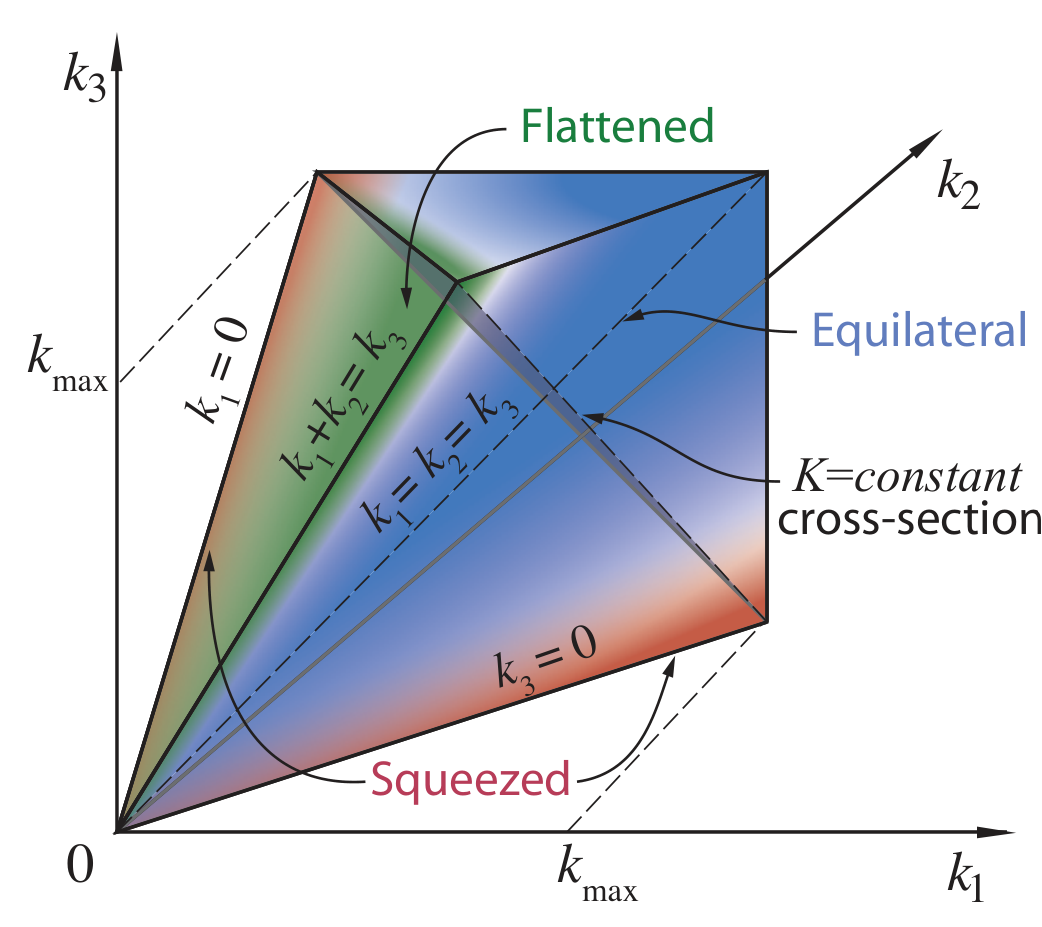
\includegraphics[width=.75\columnwidth]{plots/tetrapyd_3d_colour_split.png}}\\
    \subfloat{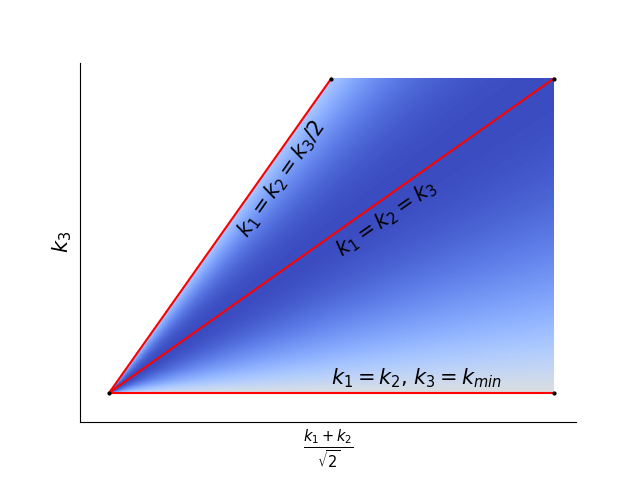
\includegraphics[width=.75\columnwidth]{plots/slice_explained.png}}
\caption{
    For ease of display, we will plot the two-dimensional $k_1=k_2$ slice of the tetrapyd
    for each of our validation examples, as shown schematically here.
    Horizontal lines on this plot have
    constant $k_3$. The bottom edge is $k_3=\kmin$, the top
    edge is $k_3=\kmax$. The right edge is $k_1=k_2=\kmax$, the
    left edge is $k_1=k_2=k_3/2$, i.e.\ the limit imposed by the triangle condition.
    Plotted in red (in the right hand plot) from top-left to bottom-right,
    are the flattened, equilateral and squeezed limits. For comparison,
    half of the tetrapyd is shown in the three-dimensional plot above
    (which was made by \textcolor{red}{WHOM?}).
}\label{slice_explained}
\end{figure}


We display the phenomenology of our various validation examples
by plotting slices through the tetrapyd, as detailed in figure~\ref{slice_explained}.
Along with the phenomenology plots we plot the residual
(with respect to the totally converged result)
on the same slice, relative to the magnitude of the shape~\eqref{rep_val}.
We emphasise that while these plots display slices through the
tetrapyd, our actual result describes the shape function on the
entire three-dimensional volume of the tetrapyd, and
we measure our convergence over this whole space.

While one of the main advantages of this method is its direct link
to the CMB, in this section we only concern ourselves with validating the
code, not the observational viability of the scenarios considered.
We focus on accurately and efficiently calculating the primordial
tree-level comoving bispectrum, validating on models popular in the
literature.
\subsection{Quadratic slow-roll}
The first model we will consider is slow-roll inflation
on a quadratic potential~\eqref{eq:quadratic_potential}.
We consider two scenarios, both with $m=6\times10^{-6}$.
The first is deep in slow-roll, which we achieve by choosing
$\phi_0=1000$; then, choosing $\phi'_0$ according to the
slow-roll approximation, we get
$\frac{1}{2}\phi'^2=\varepsilon\approx0.2\times10^{-5}$.
We can then choose the initial value for $H$ to
satisfy the Friedmann equation to sufficient precision.
The second scenario is chosen to have a value for $n_s^{*}-1$
consistent with the $\textit{Planck}$ result,
by choosing $\phi_0=16.5$, so that $\varepsilon\approx0.8\times10^{-2}$.
The shapes are shown in figure~\ref{slice_plot_malda}.


We choose the first scenario to have such a small value of $\varepsilon$
so that we can use Maldacena's shape~\eqref{malda_shape}
as a precision test.
Indeed, we find that it has a scaled relative difference~\eqref{relative_difference_scaled}
of $2.7\times10^{-5}$ with this shape,
contrasting a scaled relative difference
of $0.077$ with the local template~\eqref{local_shape}.
This confirms that our methods and our implementation in code can accurately
pick up this basic type of featureless non-Gaussianity.


For the second scenario, we cannot validate on
Maldacena's shape~\eqref{malda_shape} or the
local template~\eqref{local_shape},
as for $\epsilon\approx0.8\times10^{-2}$ we only expect
these templates to match the true result to percent level accuracy.
Indeed, we find that our result has a correlation of $0.998$
with both~\eqref{malda_shape} and~\eqref{local_shape},
corresponding (in the sense of~\eqref{relative_difference_scaled})
to a relative difference of $6\%$,
as expected.
Instead, we validate this model using
the squeezed limit test described above,
verifying our result to $0.05\%$.


This is a validation of the convergence of our basis,
reaffirming the template decomposition results of figure~\ref{fig:recon_malda_dbi}
in the setting of the in-in formalism.
It is also a stringent validation of our methods of including the higher-order
coefficients, as insufficient care taken in the early-time sections of
integrals~\eqref{inin_kindep}, or in including the spatial derivatives
from $\Hint$, could have easily swamped the $\Pmax=45$ result.


\begin{figure}[!pth]
\centering
    \subfloat{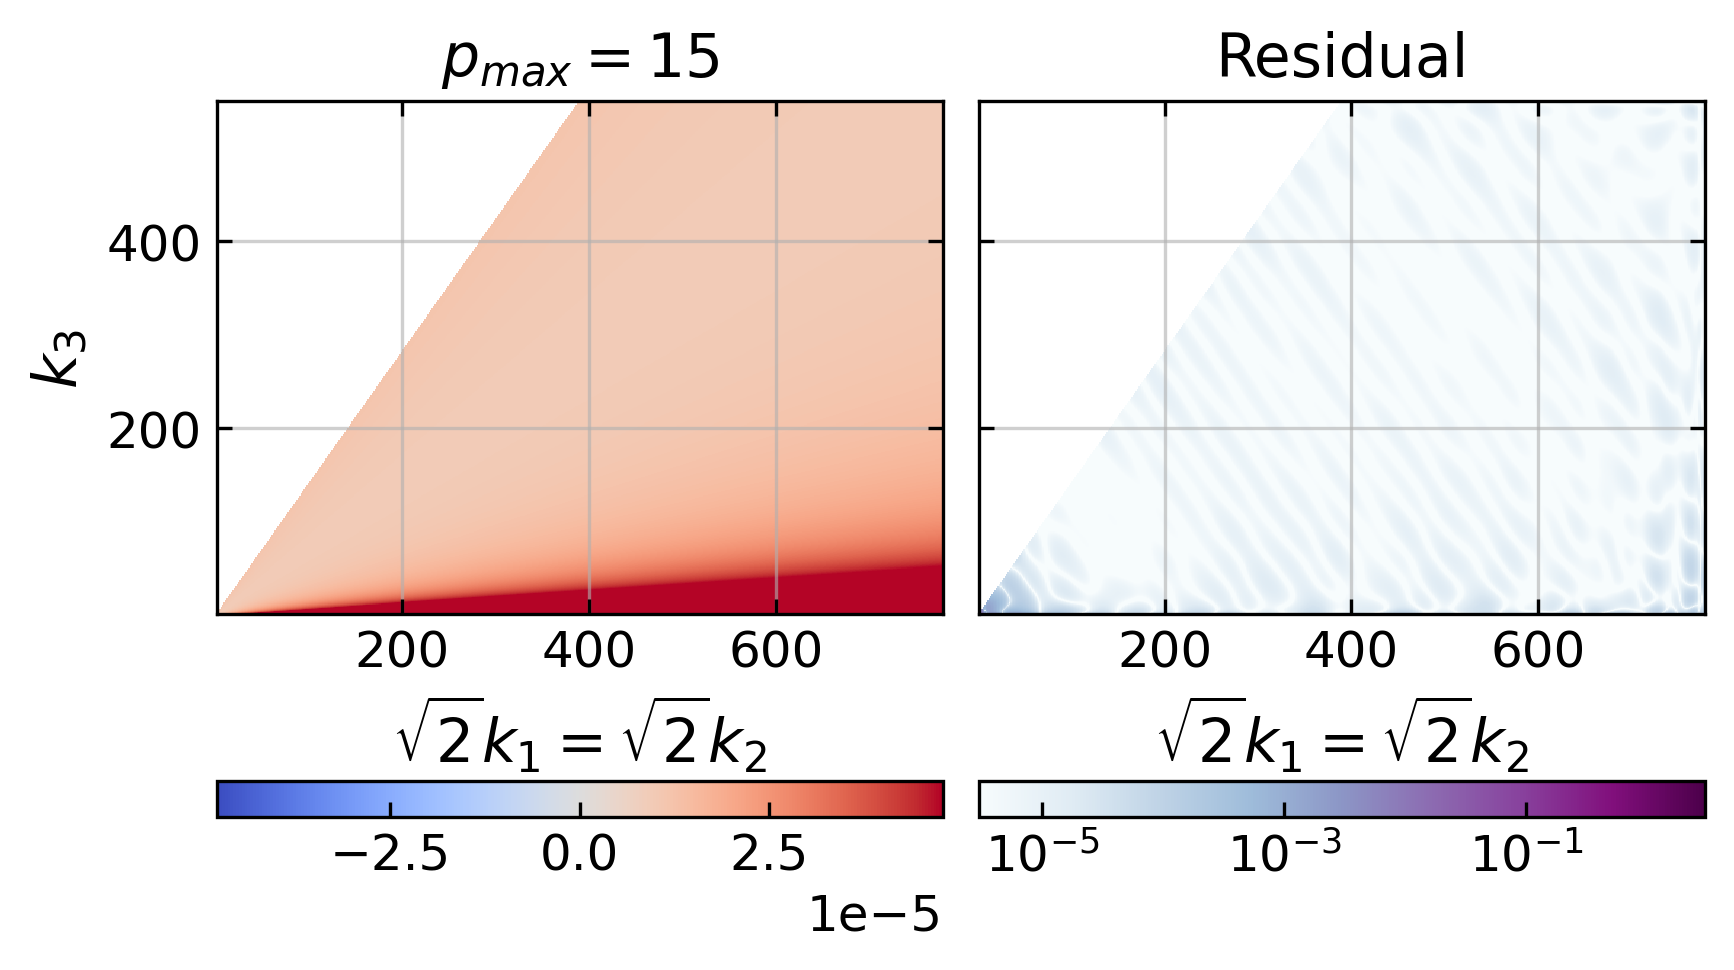
\includegraphics[width=0.99\columnwidth]{plots/tetra_slice_malda_sr_hq.png}}\\[-2ex]
    \subfloat{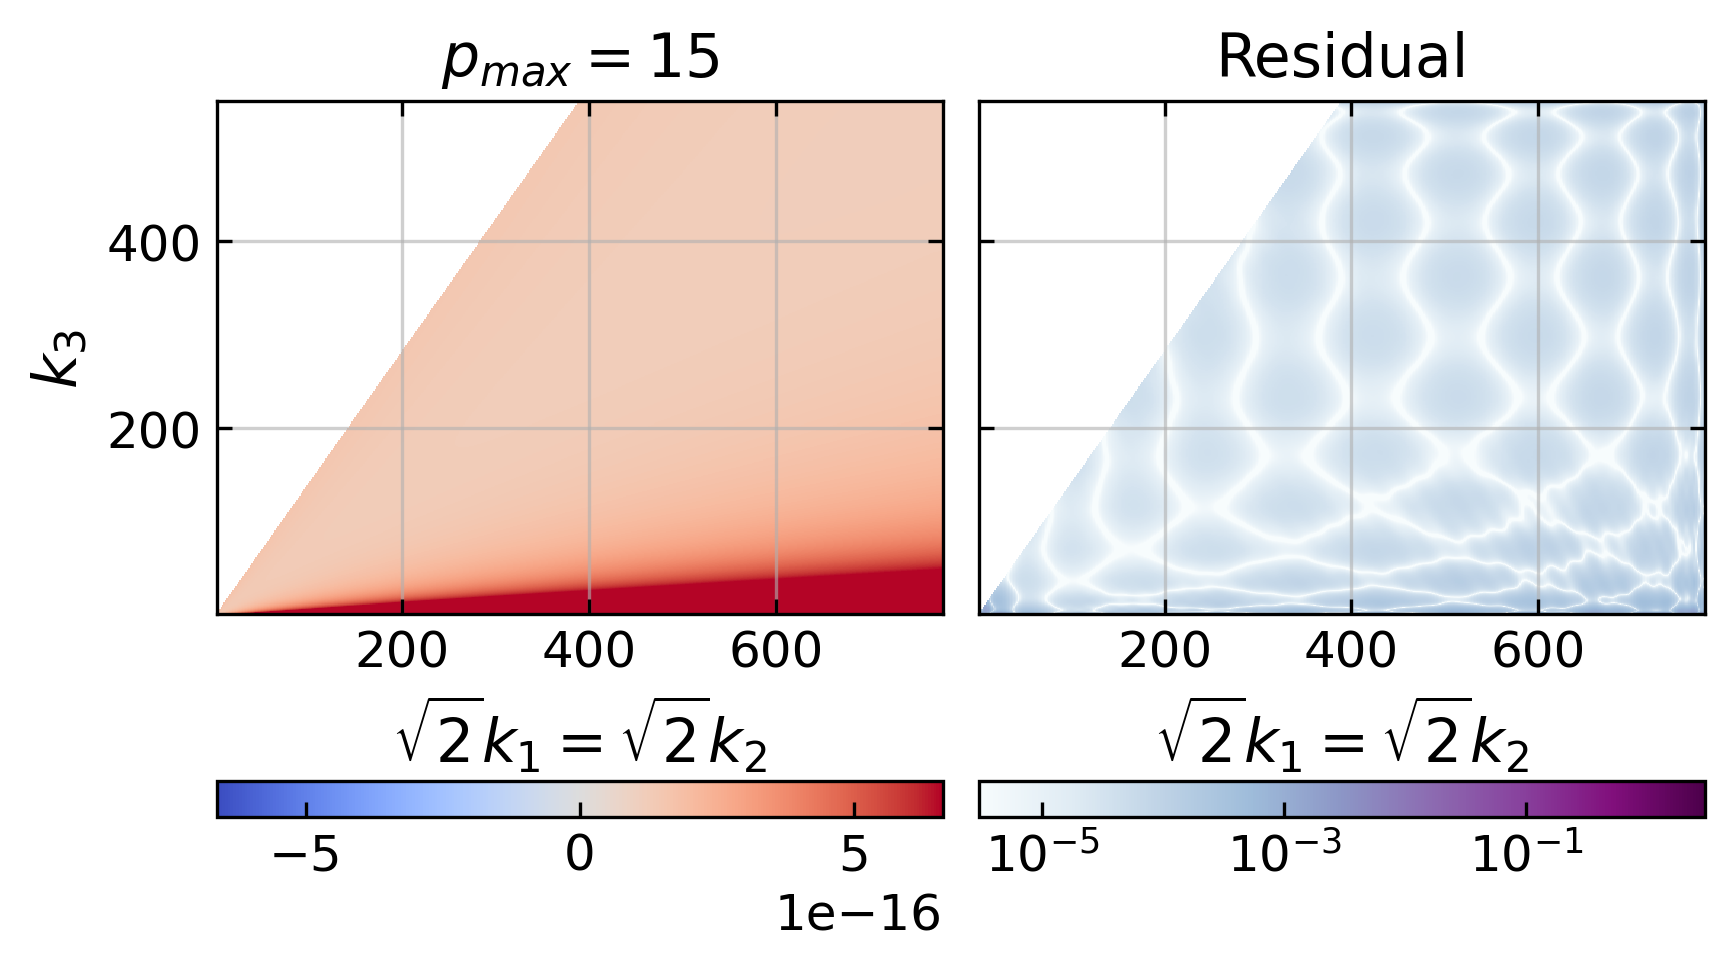
\includegraphics[width=0.99\columnwidth]{plots/tetra_slice_malda_hq.png}}
\caption{
    A canonical single-field model on a quadratic
    potential~\eqref{eq:kink_potential},
    slowly-rolling with $\varepsilon\approx2\times10^{-6}$
    in the top plot, and $\varepsilon\approx0.8\times10^{-2}$
    in the lower plot.
    This shape is dominated by its squeezed limit,
    and has a scale dependence determined by $\varepsilon$,
    very small in the top plot and ``realistic'' in the
    lower plot, relative to the $\textit{Planck}$ power spectrum.
    The first scenario converges well in the $\Linvk$ basis,
    with a relative difference of $2.7\times10^{-5}$
    %2.6764e-05
    between $\Pmax=45$ and $\Pmax=15$.
    The second scenario converges well in the $\Lnsboth$ basis
    (with $n_s^{*}-1 = -0.0325$),
    with a relative difference of $7.9\times10^{-5}$
    % 7.9047e-05
    between $\Pmax=45$ and $\Pmax=15$.
}\label{slice_plot_malda}
\end{figure}


\subsection{DBI inflation}
Next, we show results for a similar pair of scenarios for DBI inflation.
We choose $V_{0}={5.2\times10^{-12}}$~% and $\beta_{IR}=0.29$
with $m=\sqrt{0.29V_0/3}$
in~\eqref{eq:dbi_action} and~\eqref{eq:dbi_warp}.
We choose $\phi_0=0.41$, and then the starting condition
for $H$ according to the slow-roll approximation,
allowing us to choose $\phi'_0$ such that the Friedmann
equation is satisfied to sufficient precision.
The first scenario is deep in slow-roll, with $\lambda_{DBI}=1.9\times10^{18}$, while
the second scenario saturates the $\textit{Planck}$
limit on $c_s$, with $\lambda_{DBI}=1.9\times10^{15}$.
The resulting shapes are shown in figure~\ref{slice_plot_dbi}.


The scenario deep in slow-roll has a error of $0.082\%$
%0.0008243088
relative to the DBI shape~\eqref{dbi_shape},
and $13\%$
%0.1313763404
relative to the equilateral template~\eqref{equil_shape}.
The second scenario has a relative error of $2.9\%$
%0.0293218555
with the scale-invariant DBI shape, and $14\%$ with the equilateral template.
%0.1391026565
Including some scale dependence in the template,
using~\eqref{dbi_ns_shape}, we get a relative error of $0.27\%$.
%0.0026744179
On the line defined by~\eqref{sqz_line},
both scenarios have a sub-percent difference from the
consistency condition, with respect to the equilateral configurations,
which decreases when configurations with a larger $k_S/k_L$ are considered.

Including the minimal information of an individual, approximately
representative value of $n_s^{*}-1$
in $\Lnsboth$ allows us to converge to these smooth shapes quickly
and robustly, overcoming the tetrapyd-vs-cube difficulties described
in~\ref{chapter:decomp}. Our accurate match to these shapes validates our
implementation in code, and the ability of the method
(and our basis in particular) to capture very different types of
bispectrum shapes, local and equilateral.


\begin{figure}[!pth]
\centering
    \subfloat{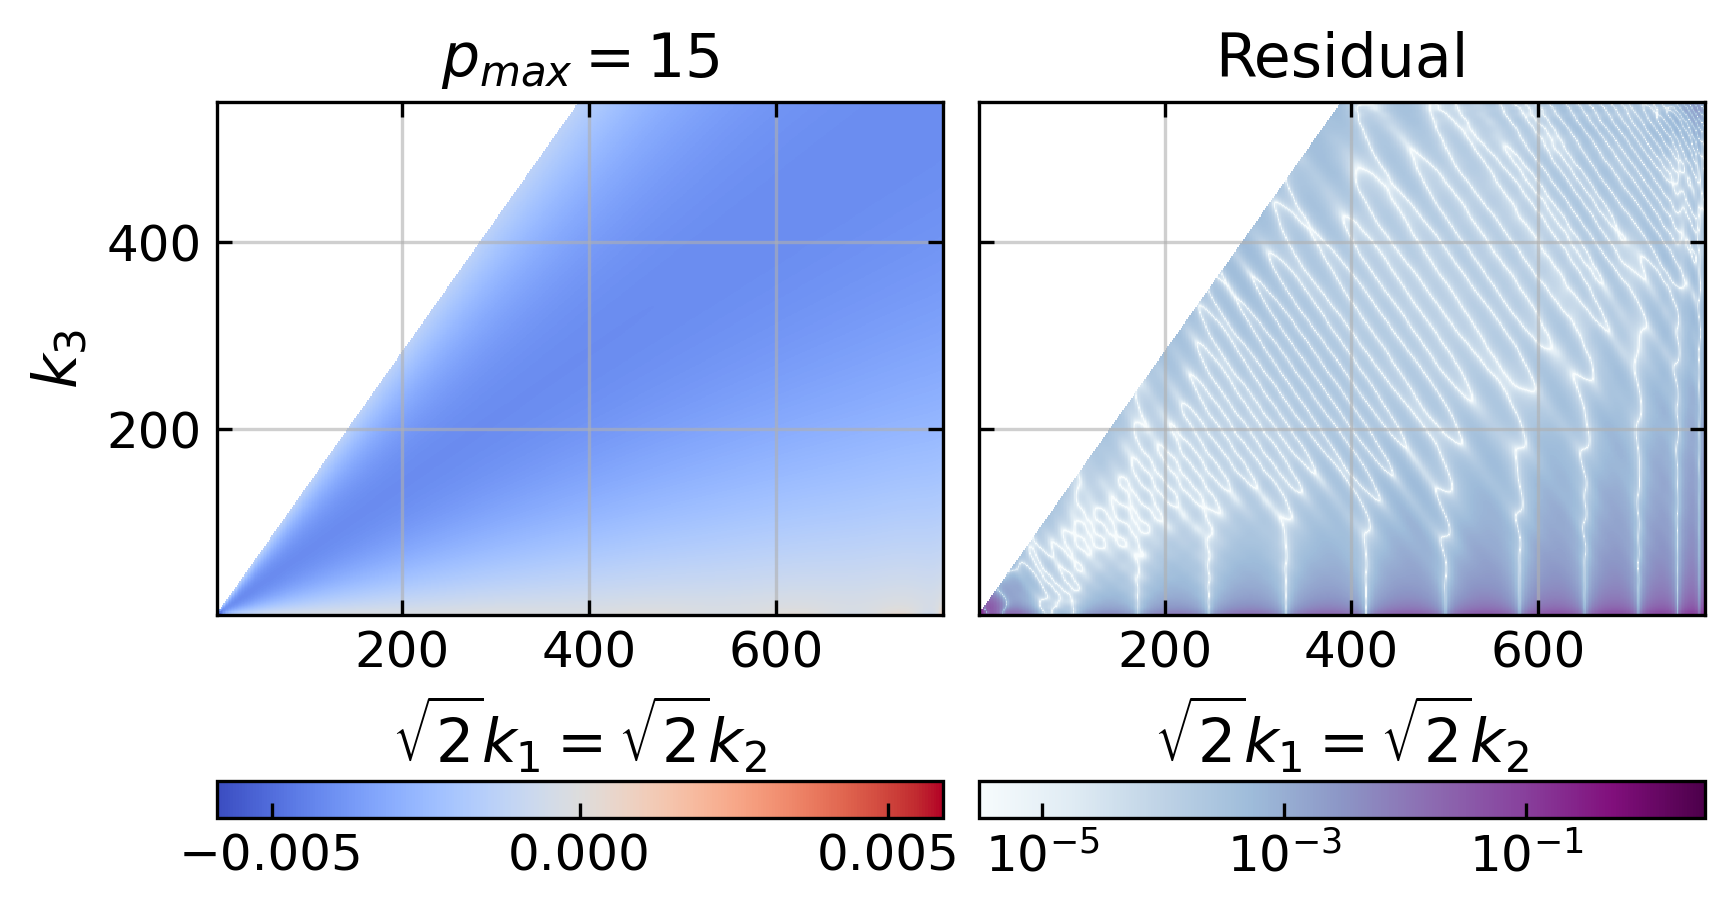
\includegraphics[width=0.99\columnwidth]{plots/tetra_slice_dbi_sr_hq.png}}\\[-2ex]
    \subfloat{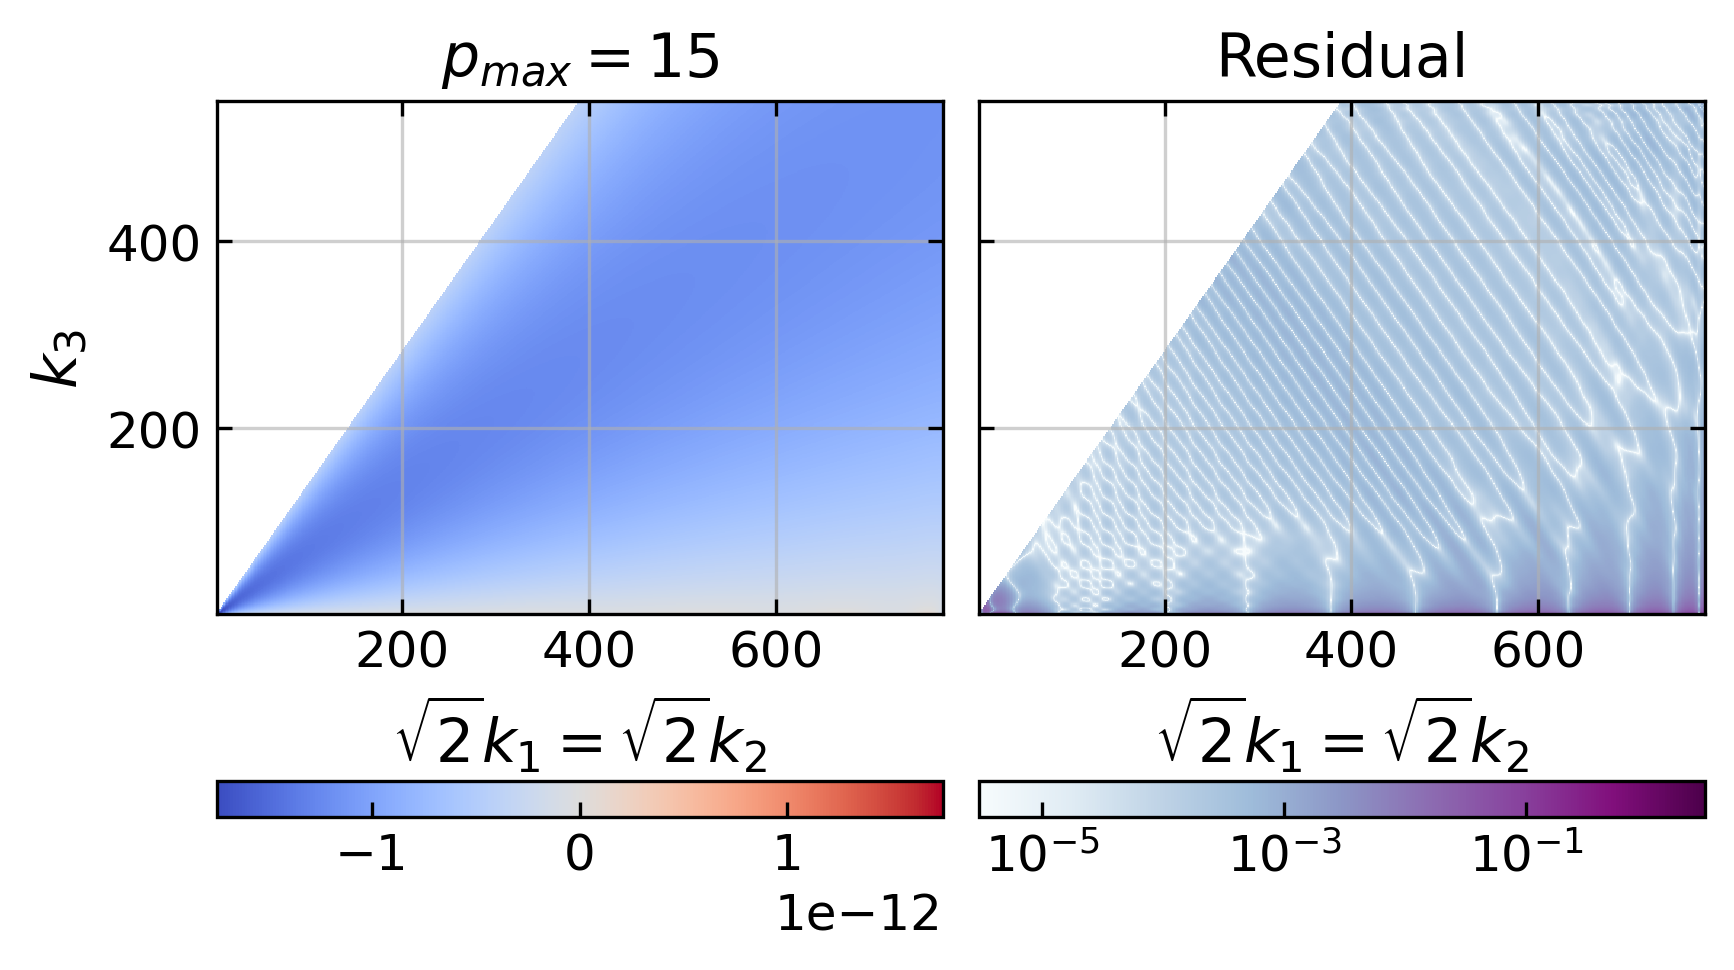
\includegraphics[width=0.99\columnwidth]{plots/tetra_slice_dbi_hq.png}}
\caption{
    The upper plot shows the shape function for a DBI model
    deep in slow-roll. We set
    $\lambda_{DBI}$ in~\eqref{eq:dbi_warp} to $1.9\times10^{18}$,
    obtaining a scenario with $\varepsilon\approx1.9\times10^{-6}$ and
    $c_s=2.3\times10^{-3}$.
    This shape is dominated by its equilateral configurations,
    and has only a slight scale dependence.
    It converges well in the $\Linvk$ basis,
    with a relative difference of $2.1\times10^{-3}$
    % 2.1203e-03
    between $\Pmax=45$ and $\Pmax=15$.
    The lower plot shows a DBI model that saturates the {\it{Planck}}
    limit on $c_s$. We set
    $\lambda_{DBI}$ in~\eqref{eq:dbi_warp} to $1.9\times10^{15}$,
    obtaining a scenario with $\varepsilon\approx8.0\times10^{-5}$ and
    $c_s=8.0\times10^{-2}$.
    This shape is also dominated by its equilateral configurations,
    but has a scale dependence consistent with the measured
    power spectrum.
    It converges well in the $\Lnsboth$ basis
    (with $n_s^{*}-1 = -0.0325$),
    with a relative difference of $1.1\times10^{-3}$
    % 1.1461e-03
    between $\Pmax=45$ and $\Pmax=15$.
}\label{slice_plot_dbi}
\end{figure}


\subsection{Step features}
Moving on from simple featureless bispectra, we present the results of
our validation tests on non-Gaussianity coming from a sharp feature in the potential.
We use the same parameters for the quadratic potential as in the
second scenario in fig~\ref{slice_plot_malda}.
In~\eqref{eq:kink_potential}
we fix $d=1\times10^{-2}$ and $\phi_{f}=15.55$
(as with the second canonical quadratic example, $\phi_0=16.5$).
Figure~\ref{slice_plot_tanh}
shows results for the shape function for two step sizes,
$c=5\times10^{-5}$ and $c=5\times10^{-3}$.
The resulting shape for small step sizes contains simple oscillations,
linear in $k_1+k_2+k_3$,
whose phase is almost constant across the tetrapyd.
When the step size is small, as expected,
our result matches the analytic result of~\cite{adshead},
presented there in equations (48), (54), (55).
We plot a comparison of the result of~\cite{adshead} and our result
in figure~\ref{fig:tanh_scan}.
For larger step size, we check the squeezed limit in figure~\ref{fig:tanh_sqz},
where we also show point tests against the PyTransport code.
Across this range of step sizes, for the resulting shapes we obtain
a full tetrapyd convergence test result
(between $\Pmax=65$ and $\Pmax=35$)
of between $0.17\%$ and $0.15\%$ and
we verify the squeezed limit test to better than $0.5\%$.

These examples show the utility of our methods in
calculating bispectra with non-trivial shape and scale dependence,
going beyond the simple examples of~\cite{Funakoshi}.
They validate the calculation of the high order coefficients,
and show that our code as implemented can handle sharp deviations from slow-roll,
generating non-Gaussianity around horizon crossing.


\begin{figure}[!pth]
\centering
    \subfloat{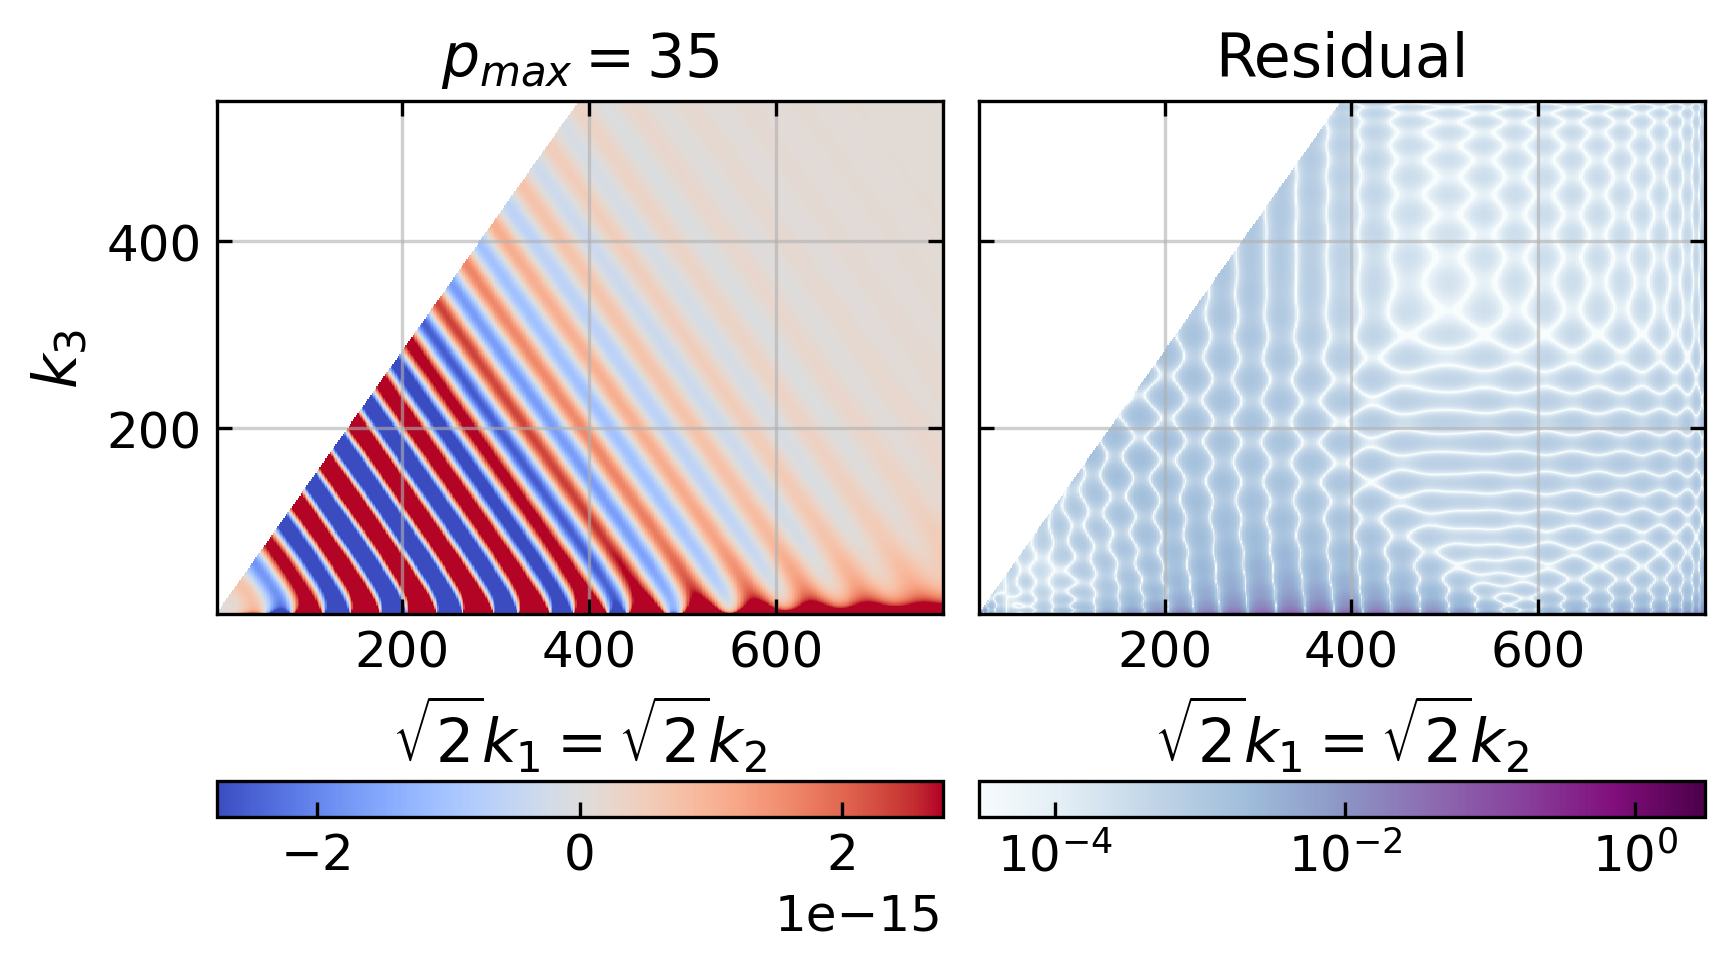
\includegraphics[width=0.99\columnwidth]{plots/tetra_slice_tanh_small_hq.png}}\\[-2ex]
    \subfloat{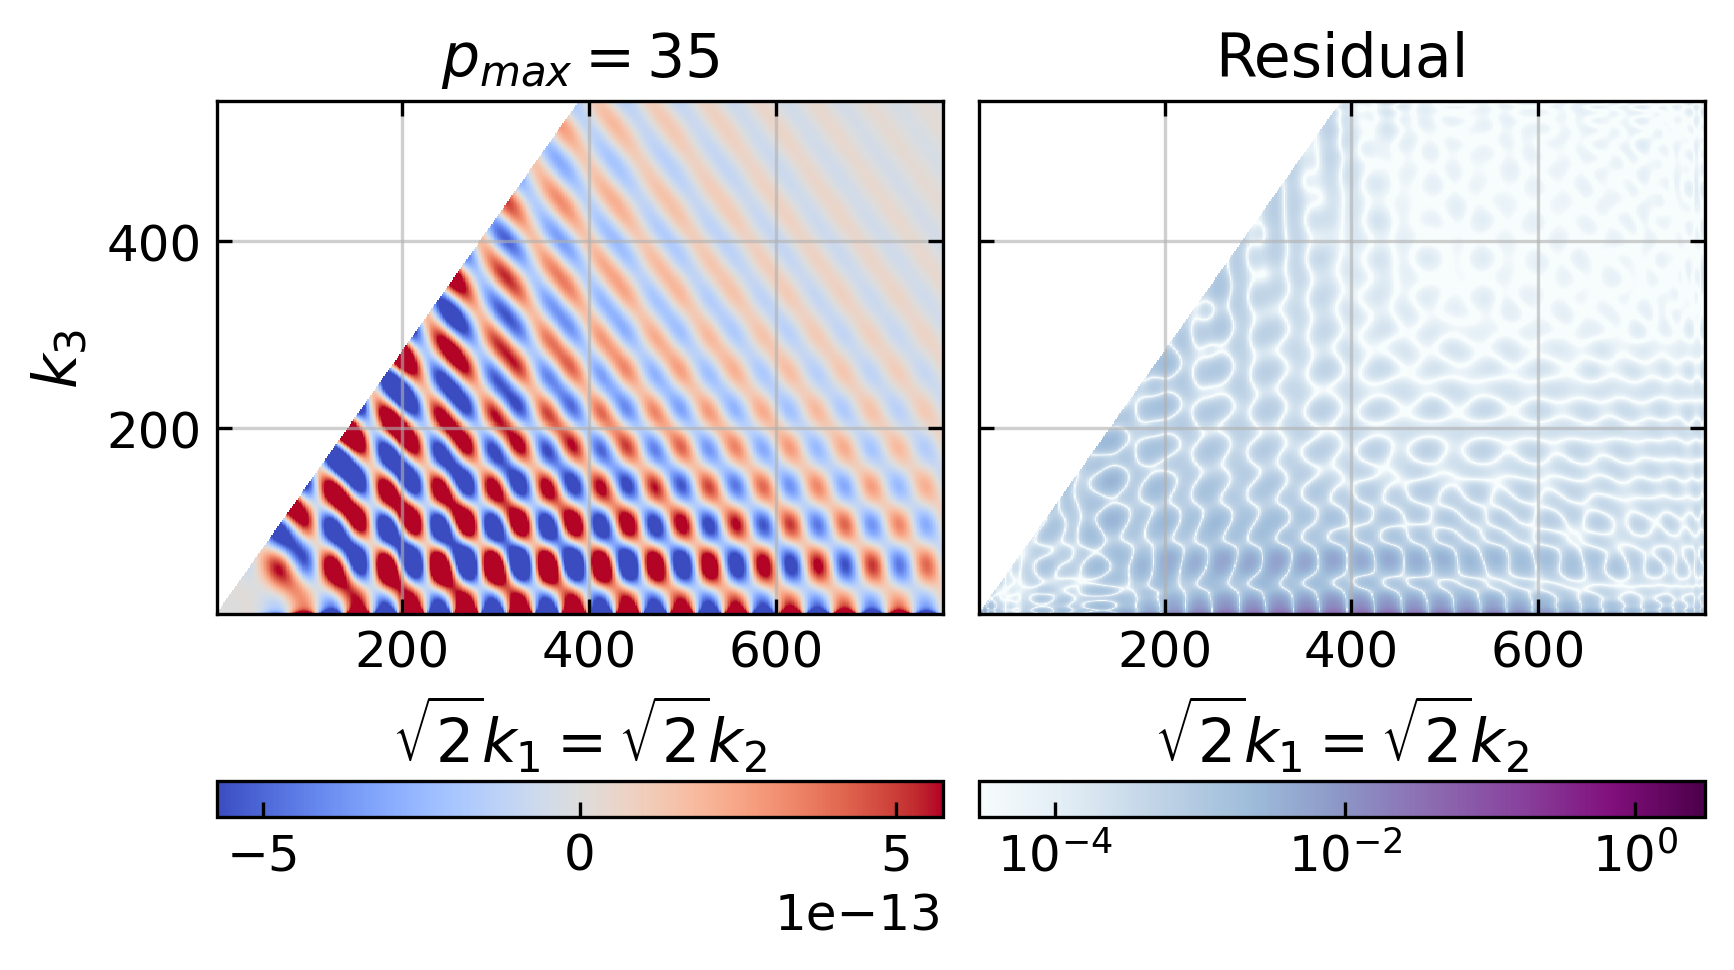
\includegraphics[width=0.99\columnwidth]{plots/tetra_slice_tanh_large_hq.png}}
\caption{
    The tree-level shape function of a feature
    model~\eqref{eq:kink_potential}, shown for step sizes of
    $c=5\times10^{-5}$ (upper plot)
    and $c=5\times10^{-3}$ (lower plot).
    The corresponding expansion parameter values of~\cite{adshead},
    ${\mathcal{C}=6c/(\varepsilon+3c)}$, are $0.035$
    and $1.3$.
    For the smaller step size, the oscillations are almost entirely functions of $K=k_1+k_2+k_3$,
    except for a phase difference in the squeezed limit.
    The dependence is more complicated for $\mathcal{C}=1.3$,
    however our result still converges well.
    In the $\Lnsboth$ basis, with $n_s^{*}-1 = -0.0325$,
    the results have a relative difference of $1.6\times10^{-3}$
    and $1.5\times10^{-3}$, respectively,
    % 1.6406e-03
    % 1.6418e-03
    % 1.4856e-03
    between $\Pmax=65$ and $\Pmax=35$.
}\label{slice_plot_tanh}
\end{figure}
\begin{figure*}
    %\centering
    \subfloat{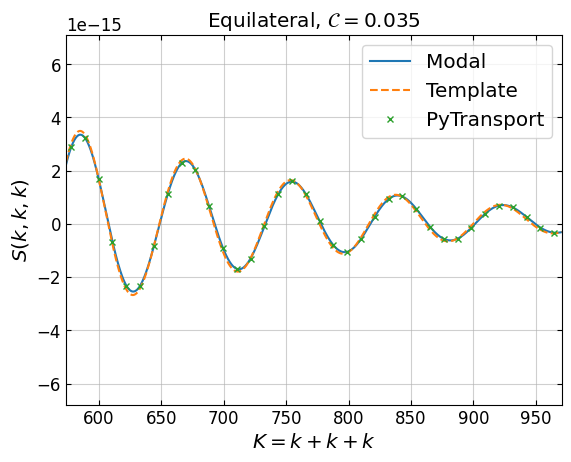
\includegraphics[width=0.49\columnwidth]{plots/tanh_5e-05_equil}}
    \hfill
    \subfloat{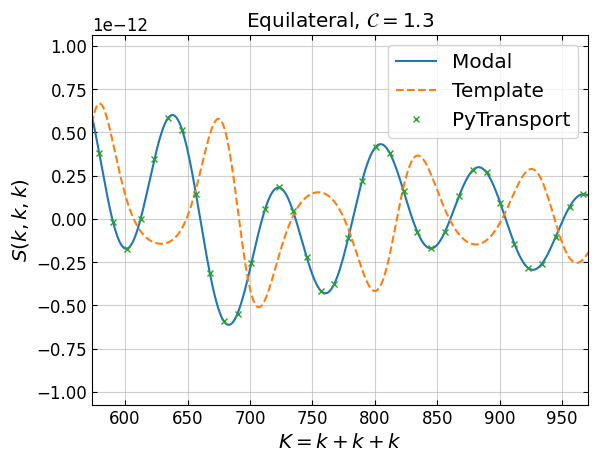
\includegraphics[width=0.50\columnwidth]{plots/tanh_5e-03_equil}}
    \vskip\baselineskip
    \subfloat{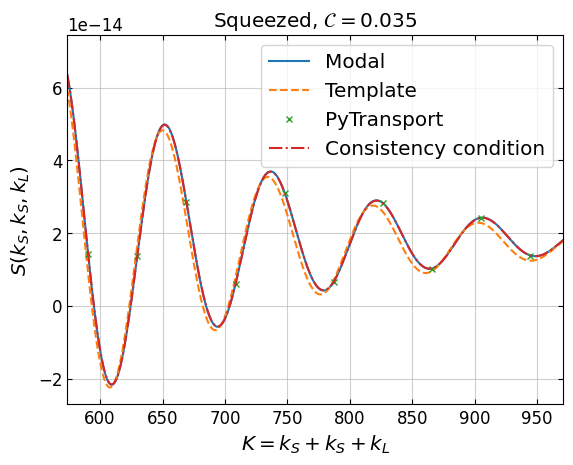
\includegraphics[width=0.49\columnwidth]{plots/tanh_5e-05_sqz}}
    \hfill
    \subfloat{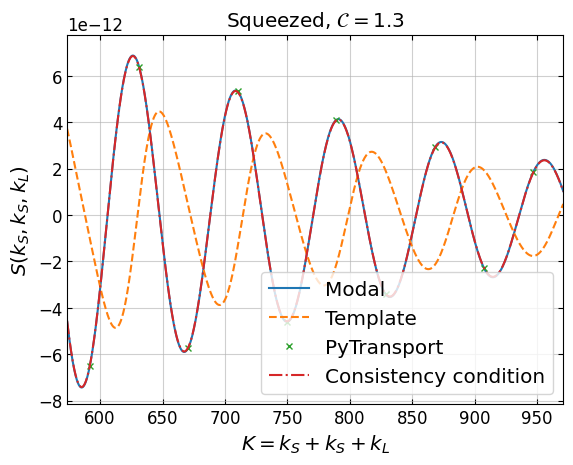
\includegraphics[width=0.49\columnwidth]{plots/tanh_5e-03_sqz}}
\caption{
	In the equilateral limit for the feature models (the top two figures) we validate our modal result
	against the PyTransport result. In the squeezed limit (the bottom two figures)
	we validate against PyTransport, and the consistency condition.
	In both limits, for both step sizes shown, we find excellent agreement.
	For the small step size (the two plots to the left), we additionally
	see a good match to the template of~\cite{adshead}. For the larger step size,
	the template amplitude is still accurate,
    but no longer captures the detailed shape information.
    This validates our code on non-Gaussianity generated by sharp
    features, and illustrates the general usefulness of our method.
	Our numerical results are accurate in a broader range than
	approximate templates, but are still smooth separable functions,
	unlike the results of previous numerical codes.
}\label{fig:tanh_sqz}
\end{figure*}
\begin{figure}[!pth]
\centering
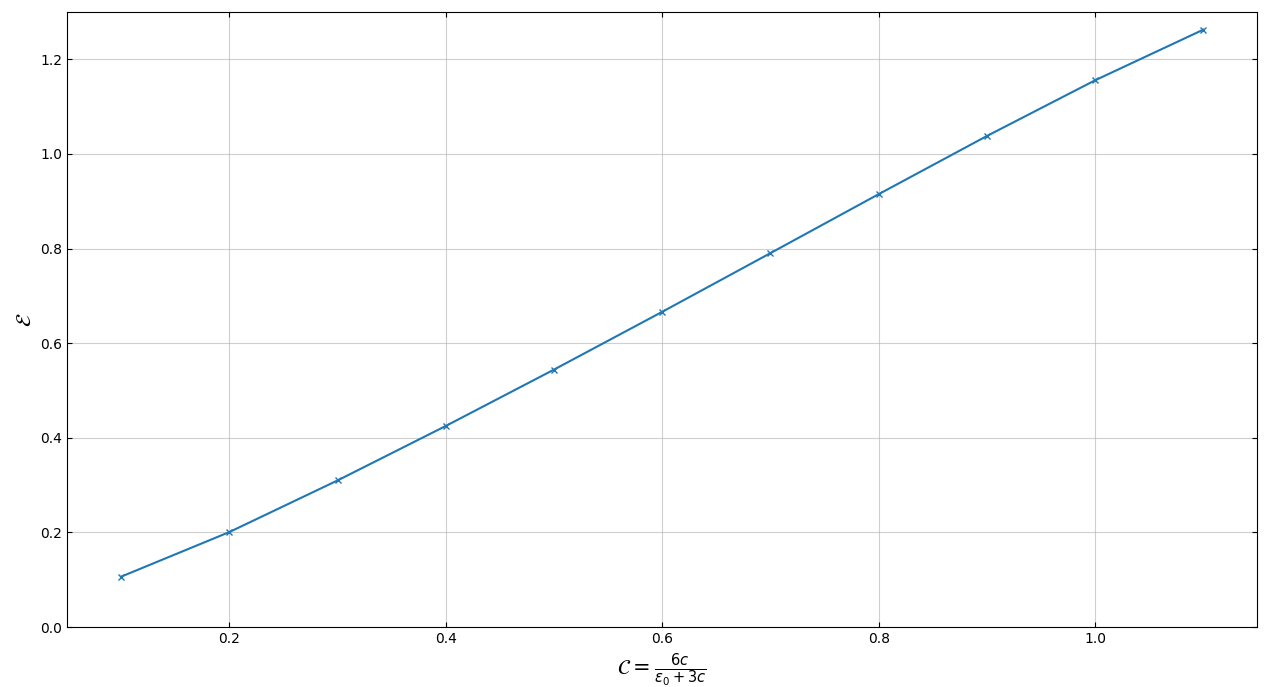
\includegraphics[width=.75\columnwidth]{plots/tanh_scan_C_cropped.png}
\caption{
    We sample more shapes with step sizes between the two
    feature models shown in figure~\ref{slice_plot_tanh}.
    We plot the relative difference,
    integrated over the full tetrapyd
    in the sense of~\eqref{relative_difference},
    between the modal result and the analytic template of~\cite{adshead},
    as a function of the template parameter $\mathcal{C}=\frac{6c}{\varepsilon_0+3c}$
    (where $c$ is the step size and $\varepsilon_0$ is the value of the slow-roll parameter
    $\varepsilon$ at $\phi_{step}$ when $c=0$). We test our result by verifying
    the squeezed limit consistency
    condition to better than 1\% throughout (not shown). The number of oscillations in the
    $k$-range is determined by the conformal time at which the kink in~\eqref{eq:kink_potential}
    occurs, which is kept constant across this scan. The width of the feature was also kept constant.
}\label{fig:tanh_scan}
\end{figure}

\subsection{Resonance features}
Now we further validate our code against two
resonance models. In contrast to the previous sharp kink,
this feature is extended, requiring precision at earlier times.
The first, shown in figure~\ref{pytr_comparison_min},
is a model with a canonical kinetic term, on a
quadratic potential with a superimposed
oscillation~\eqref{eq:resonant_potential}.
We take $bf=10^{-7}$, and $f=10^{-2}$.
The resulting bispectrum has oscillations logarithmic in $k_1+k_2+k_3$.
In figure~\ref{pytr_comparison_min} we see the excellent agreement
between our result and the PyTransport result, once initial conditions
in both codes are set early enough to achieve convergence.
This validates the code on non-Gaussianity generated deeper
in the horizon. Note the change of phase in the squeezed limit,
though this is expected to be unobservable.
We obtain a full tetrapyd convergence test result
(between $\Pmax=65$ and $\Pmax=35$)
of $0.93\%$, a squeezed limit test result of $1.1\%$
(along the line defined by~\eqref{sqz_line}),
and a relative difference of $3.0\%$ with respect to the
PyTransport result,
although this is only integrated over the two-dimensional slice presented in
figure~\ref{pytr_comparison_min}.


The time taken for the PyTransport code (per configuration) varies by a factor of around forty
between the equilateral limit and the squeezed limit,
as we show in figure~\ref{pytr_comparison_min}.
While the PyTransport code is extremely fast at calculating the shape function
for a single $k$-configuration,
to obtain this two-dimensional slice through the tetrapyd took around seven hours;
to obtain the shape function on the full three-dimensional tetrapyd would take much longer.
In contrast, our code took less than an hour on the same machine to calculate
the full shape function, not limited to the shown slice.
The overall speed increase is, therefore, a factor on the order of $10^2$ to $10^3$
for the full shape information, speaking only on the level of primordial
phenomenology, in addition to the advantage that our result is in a form
designed to be compared with observation.
We expect that our implementation can be optimised beyond this.


The second scenario we consider here also has an
oscillation superimposed on its potential, but this time
is a non-canonical model, the DBI model.
The resulting bispectrum is shown in figure~\ref{slice_plot_dbi_reso}.
Note especially the out-of-phase oscillations in the flattened limit,
which are potentially observable.
For the purpose of displaying this phenomenology, we place a window
on the oscillation in the potential, smoothing out the resulting oscillations
in the shape at low $k_1+k_2+k_3$, to aid convergence.
This validates our code on non-Gaussianity generated by deviations from Bunch-Davies
behaviour~\cite{chen_folded_resonant,features_bartolo}.
We obtain a convergence test result (between $\Pmax=65$ and $\Pmax=35$)
of $0.15\%$, and a squeezed limit test result of $6.5\%$.


\begin{figure}[!pth]
\centering
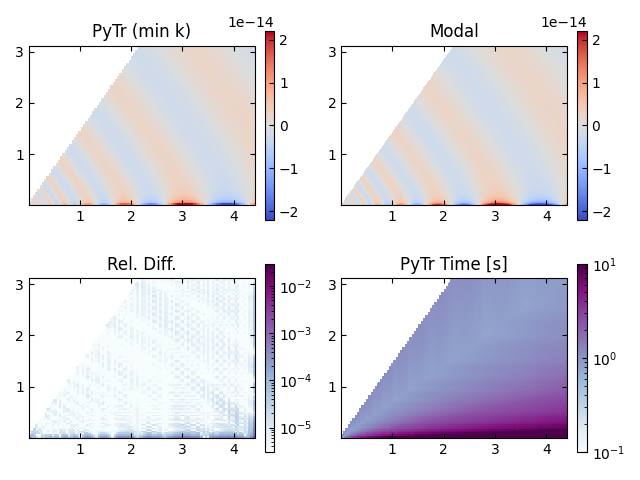
\includegraphics[width=0.99\columnwidth]{plots/slice_min_100.png}
\caption{
    Resonance on a quadratic potential~\eqref{eq:resonant_potential},
    testing our result using point tests against the
    PyTransport code.
    The logarithmic oscillations in the shape function are generated by periodic
    features deep in the horizon.
    The differences between our result and the PyTransport result
    are sufficiently small throughout that we can consider this
    a validation of our code on non-Gaussianity generated by periodic
    features deep in the horizon.
    In the $\Lnsboth$ basis, with $n_s^{*}-1 = -0.0325$,
    our result has a relative difference of $9.6\times10^{-3}$
    % 9.5587e-03
    between $\Pmax=65$ and $\Pmax=35$.
}\label{pytr_comparison_min}
\end{figure}

\begin{figure}[!pth]
\centering
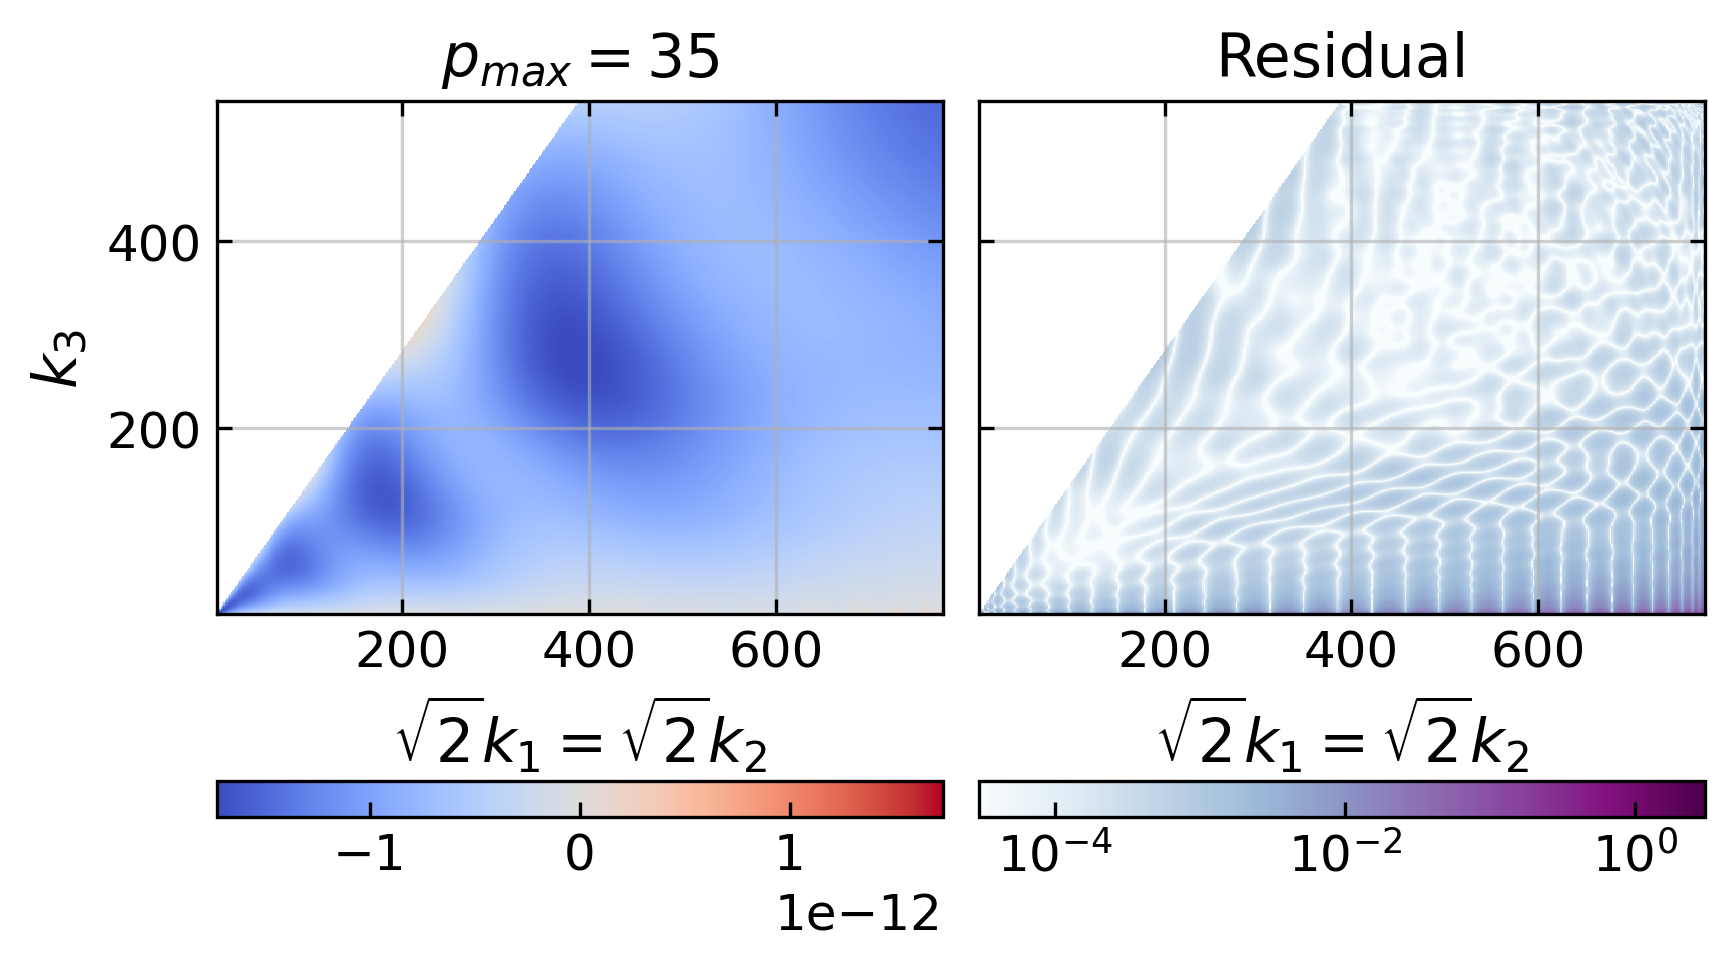
\includegraphics[width=0.99\columnwidth]{plots/tetra_slice_dbi_reso_bump_hq_coolwarm.png}
\caption{
    Non-Gaussianity generated by periodic
    features in a DBI model, including a phase difference
    in the flattened limit as described in~\cite{chen_folded_resonant}.
    For the purposes of demonstrating the phenomenology,
    we have placed an envelope on the oscillations in the potential
    to aid convergence.
    In the $\Lnsboth$ basis, with $n_s^{*}-1 = -0.0325$,
    the result has a relative difference of $1.9\times10^{-3}$
    % 1.9482e-03
    between $\Pmax=65$ and $\Pmax=35$.
}\label{slice_plot_dbi_reso}
\end{figure}
\newpage
\section{Speed comparison vs PyTransport.}
    Something BINGO can't do?
\newpage
%\section{TO-DO: Map distinguishability of templates at primordial level}
%    To determine where to usefully scan.
%\newpage
\section{Conclusion}
    \subsection{My methods have been validated on interesting examples}
    Words
    \subsection{Separable methods for high orders and features for the first time}
    Words
    \subsection{Full shape info far faster than previous numerical methods}
    Words

%\bibliographystyle{unsrt}
%\bibliographystyle{JHEP}
%\bibliography{thesis}


%%%%%%%%%%%%%%%%%%%%%%%%%%%%%%%%%%%%%%%%%%%%%%%%%%%%%%%%%%%%%%%%%%%%%%%%%%%%%%%%
%% Chapter 3:
%%
%%\chapter{Primordial results}
\section{Abstract}\label{sec:primordial_abstract}
\section{High $p_{max}$}\label{sec:high_pmax}
\subsection{How high can I push $p_{max}$?}
How high can I push $p_{max}$?



%%%%%%%%%%%%%%%%%%%%%%%%%%%%%%%%%%%%%%%%%%%%%%%%%%%%%%%%%%%%%%%%%%%%%%%%%%%%%%%%
%% Chapter 4:
%%
%\newcommand{\eps}{\epsilon}
\newcommand{\Pmax}{p_\text{max}} 	
\newcommand{\Hint}{H_{int}}
\newcommand{\kbar}{\bar{k}}
\newcommand{\Delk}{\Delta}
\newcommand{\Sumk}{\Sigma}
\newcommand{\Qrot}{Q_{pq}(\tau_s)}
\newcommand{\shapecor}{\mathcal{S}}
\newcommand{\ampcor}{\mathcal{A}}
\newcommand{\totalcor}{\mathcal{E}}
\newcommand{\threeLs}{L_p(\kbar_1)L_q(\kbar_2)L_r(\kbar_3)}
\newcommand{\threePs}{P_p(\kbar_1)P_q(\kbar_2)P_r(\kbar_3)}
\newcommand{\threeQs}{Q_p(k_1)Q_q(k_2)Q_r(k_3)}
\newcommand{\Lbasic}{\mathcal{P}_0}
\newcommand{\Linvk}{\mathcal{P}_1}
\newcommand{\Lnsinv}{\mathcal{P}^{n_s}_1}
\newcommand{\Lnsboth}{\mathcal{P}^{n_s}_{01}}
\newcommand{\Linvksq}{\mathcal{P}_2}
\newcommand{\Lns}{\mathcal{P}^{n_s}_2}
\newcommand{\Fbasic}{\mathcal{F}_0}
\newcommand{\Finvk}{\mathcal{F}_1}
\newcommand{\Finvksq}{\mathcal{F}_2}
\newcommand{\quadpot}{V_{\phi^2}(\phi)}
%\newcommand{\threeqs}{q_p(\kbar_1)\,q_r(\kbar_2)\,q_s(\kbar_3)}
\newcommand{\threeqs}{q_p(k_1)\,q_r(k_2)\,q_s(k_3)}
\newcommand{\threeqstilde}{q_{\tilde{p}}(k_1)\,q_{\tilde{r}}(k_2)\,q_{\tilde{s}}(k_3)}
\newcommand{\kmin}{{k_\text{min}}}
\newcommand{\kmax}{{k_\text{max}}}
\newcommand{\fnl}{f_{NL}}
\newcommand{\fnllocal}{f^{local}_{NL}}
\newcommand{\fnlequil}{f^{equil}_{NL}}
\newcommand{\fnlortho}{f^{ortho}_{NL}}

\chapter{Constraints}\label{chapter:constraints}
\section{Connecting to $\cmbbest$}
\textcolor{red}{We don't get an exact match, maybe due
to $140$ Gaussian simulations vs. Modal's $~300$.
Or perhaps it is simply a statistical fluctuation.}
    The goal here is to validate our pipeline by reproducing the $\planck$~result
    from~\cite{Planck_NG_2018}, equation (55):
    \begin{align}
        c_s^{DBI}&\ge0.079\qquad(95\%,~T~\text{only}).
    \end{align}
    We would not expect to reproduce this exactly due to
    \textcolor{red}{Lack of maps? Different approximations? Numerics?}
    Though we can estimate a reasonable disagreement by looking at
    the expected scatter between the $\planck$ estimators, and by calculating
    \textcolor{red}{$\sigma$??}.

\section{Set-up of the scan}
The potential we use is the IR one discussed in~\cite{Bean_ir_dbi} as discussed \textcolor{red}{earlier}.
See also~\cite{Chen_dbi, warp_features_dbi} for useful discussions.


    We use equation~\eqref{eq:dbi_warp}, with $\beta_{IR}\in[0.1885, 0.58]$.
    We find that $\beta_{IR}=0.331$ produces $c_s^{*}=0.0794$,
    which is close to the above constraint.
    Thus, we roughly expect to find that $\beta_{IR}<0.331$ is ruled out
    (for all the other scenario parameters held fixed).
    We also have that $\ln\left(10^{10}A_s\right)$ for each scenario
    is within $3.044\pm0.014$ across the scan,
    and that $n_s^{*}$ is within $0.9649\pm0.0042$ across the scan.
    This set-up produces a scenario with ($*$ denotes horizon crossing of the pivot scale):
%    \begin{tabular}{lrrrrrrrrrr}
%        \toprule
%        $\beta_{IR}$ &    $c_s^{*}$ &  $\varepsilon_s^{*}$ &   $\varepsilon^{*}$ &   $n_s^{*}$ &  $n_{NG}^{*}$ &   $\phi^{*}$ &     $H^{*}$ &   $\eta^{*}$ \\
%        \midrule
%        $1.89\times 10^{-1}$  &  $1.39\times 10^{-1}$  &  $  8.57\times 10^{-3}$  &  $7.44\times 10^{-5}$  &  $-3.50\times 10^{-2}$  &  $-8.72\times 10^{-2}$  &  $5.19\times 10^{-1}$  &  $1.31\times 10^{-6}$  &  $2.63\times 10^{-2}$ \\
%        $5.80\times 10^{-1}$  &  $4.50\times 10^{-2}$  &  $  8.67\times 10^{-3}$  &  $2.31\times 10^{-4}$  &  $-3.63\times 10^{-2}$  &  $-8.99\times 10^{-2}$  &  $5.15\times 10^{-1}$  &  $1.30\times 10^{-6}$  &  $2.71\times 10^{-2}$ \\
%        \bottomrule
%    \end{tabular}
    \\
    \\
\begin{table}[h!]
  \begin{center}
    \begin{tabular}{lrrrrrrr}
        \toprule
        $\beta_{IR}$ &    $c_s^{*}$ &  $\varepsilon_s^{*}$ &   $\varepsilon^{*}$ &   $n_s^{*}$ &  $n_{NG}^{*}$\\
        \midrule
        $1.89\times 10^{-1}$  &  $1.39\times 10^{-1}$  &  $  8.57\times 10^{-3}$  &  $7.44\times 10^{-5}$  &  $9.650\times 10^{-1}$  &  $-8.72\times 10^{-2}$\\
        $5.80\times 10^{-1}$  &  $4.50\times 10^{-2}$  &  $  8.67\times 10^{-3}$  &  $2.31\times 10^{-4}$  &  $9.637\times 10^{-1}$  &  $-8.99\times 10^{-2}$\\
        \bottomrule
    \end{tabular}
    \caption{Summary of scenario parameters across the scan.}\label{tab:scan_summary}
  \end{center}
\end{table}
    \\
    \\
\begin{table}[h!]
  \begin{center}
    \begin{tabular}{lrrr}
        \toprule
        $\beta_{IR}$ &  $\phi^{*}$ &     $H^{*}$ &   $\eta^{*}$ \\
        \midrule
        $1.89\times 10^{-1}$  &  $5.19\times 10^{-1}$  &  $1.31\times 10^{-6}$  &  $2.63\times 10^{-2}$ \\
        $5.80\times 10^{-1}$  &  $5.15\times 10^{-1}$  &  $1.30\times 10^{-6}$  &  $2.71\times 10^{-2}$ \\
        \bottomrule
    \end{tabular}
    \caption{Summary of scenario parameters across the scan.}\label{tab:scan_summary2}
  \end{center}
\end{table}
    \\
    \\
    We now show convergence results for $\Lnsinv$ with $\Pmax=30$.
    For this basis the match to the template is good in the equilateral limit, but quite poor in the squeezed limit.
    \\
    \\
\begin{table}[h!]
  \begin{center}
    \begin{tabular}{lrrrr}
        \toprule
        $\beta_{IR}$ & Sum Template & Product Template & Bare Template & With $\Pmax=25$ \\
        \midrule
        $1.89\times 10^{-1}$  &  $6.15\times 10^{-3}$  &  $7.22\times 10^{-3}$  &  $5.16\times 10^{-2}$  &  $5.3\times 10^{-3}$ \\
        $5.80\times 10^{-1}$  &  $4.51\times 10^{-3}$  &  $3.63\times 10^{-3}$  &  $5.28\times 10^{-2}$  &  $2.6\times 10^{-3}$ \\
        \bottomrule
    \end{tabular}
    \caption{
        Comparing the $\Lnsinv(\Pmax=30)$ result compared to
        templates~\eqref{dbi_shape},~\eqref{dbi_sum_shape} and~\eqref{dbi_prod_shape}.
        We also refit the result with $\Lnsinv(\Pmax=25)$, and compare with the full
        result to estimate the convergence at the primordial level.
    }\label{fig:template_errors}
  \end{center}
\end{table}
    \\
    \\
    The convergence in the $\scalingbasis$ basis is better,
    falling in the range $[1.02\times 10^{-4}, 9.24\times 10^{-4}]$.
    However, for this analysis the $\cmbbest$ code had only been run for
    the $\Lnsinv$ basis. We see that it is sufficient in any case.
    When we examine the convergence to the sum~\eqref{dbi_sum_shape}
    and product~\eqref{dbi_prod_shape} scaling templates,
    in figure~\ref{fig:dbi_primodal_scan_template_corrs_log30},
    we see that neither is obviously the better match to the numerical result.
    This is due to the numerical result having a non-zero squeezed limit
    coming from the usual slow-roll suppressed local-type contributions
    (as in~\eqref{malda_shape}) which are neglected in the DBI templates.
    \\
\begin{figure}[!pth]
\centering
\includegraphics[width=\columnwidth]{dbi_scan_template_corrs_plots/dbi_primodal_scan_template_corrs_log30.png}
\caption{
    The $\scalingbasis$ basis converges well across the scan range.
    We see that the bare DBI template is a poor match to the true numerical result.
    This is mostly due to the error in the overall magnitude.
    Once this is corrected, we see that the numerical result matches the
    approximate template to better than $1\%$. As the convergence of the
    numerical result is better than $0.1\%$ for the $\scalingbasis$ basis
    we can see that sum scaling~\eqref{dbi_sum_shape} and the
    product scaling~\eqref{dbi_prod_shape} perform
    comparably in matching the numerical result. This is mostly
    due to those templates neglecting the usual slow-roll suppressed
    contributions (as in~\eqref{malda_shape}),
    which do in fact become relevant to the primordial
    bispectrum deep enough into the squeezed limit, due to their local-type shape.
}\label{fig:dbi_primodal_scan_template_corrs_log30}
\end{figure}
\begin{figure}[!pth]
\centering
\includegraphics[width=\columnwidth]{dbi_scan_template_corrs_plots/dbi_primodal_scan_template_corrs_p1ns30}
\caption{
    The $\Lnsinv$ basis is sufficiently convergent across the scan range
    to obtain the desired constraint.
    We see that the convergence error is only slightly better than the error
    in the slow-roll corrected templates.
}\label{fig:dbi_primodal_scan_template_corrs_p1ns}
\end{figure}
    \\
\section{Compare convergence at primordial level to convergence at $f_{NL}$ level}
    We will compare primordial convergence to CMB convergence,
    by comparing the $\Pmax=29$ and $\Pmax=30$ results.
    This will show that the CMB convergence is slightly better, i.e.\ that
    the squeezed limit (which is where the primordial shape converges most slowly)
    is suppressed.
    At the $\cmb$ level, the convergence is $O(10^{-5})$. What is it for $\Pmax=29$?
    at the primordial level?
    For DBI, and also for DBI resonance?
\section{Validate this convergence by reproducing $\planck$ constraint using DBI template decomposition.}
    \begin{figure}[htbp!]
        \centering
        \includegraphics[width=0.9\textwidth]{wuhyun_plots/dbi_sound_speed_scan_annotated.pdf}
        \caption{
            \textcolor{red}{To replace the above---need to make less cramped!}
            Our constraint on DBI inflation. Here $c_s^{DBI}$ is not an input parameter
            (unlike in the template case), instead it is time dependent, and the plotted
            value is taken from the horizon crossing of the pivot scale. We find that $\beta_{IR}<0.5$
            %0.464
            is outside of our $2\sigma$ confidence interval. This plot was obtained by
            scanning across values of $\beta_{IR}$ and calculating the corresponding primordial bispectra
            using $\primodal$, then projecting those bispectra onto the $\cmb$
            and comparing them to the $\planck$ $\cmb$ temperature data using
            $\cmbbest$. Since the amplitude is fixed by the scenario, we rule out a
            scenario by ruling out $f_{NL}^{DBI}=1$.
            Note that the constraint obtained for $\Pmax=30$ and $\Pmax=29$ is identical,
            so we can be confident that our constraint has converged in $\Pmax$.
        }\label{fig:dbi_sound_speed_scan}
    \end{figure}
    \begin{figure}[htbp!]
        \centering
        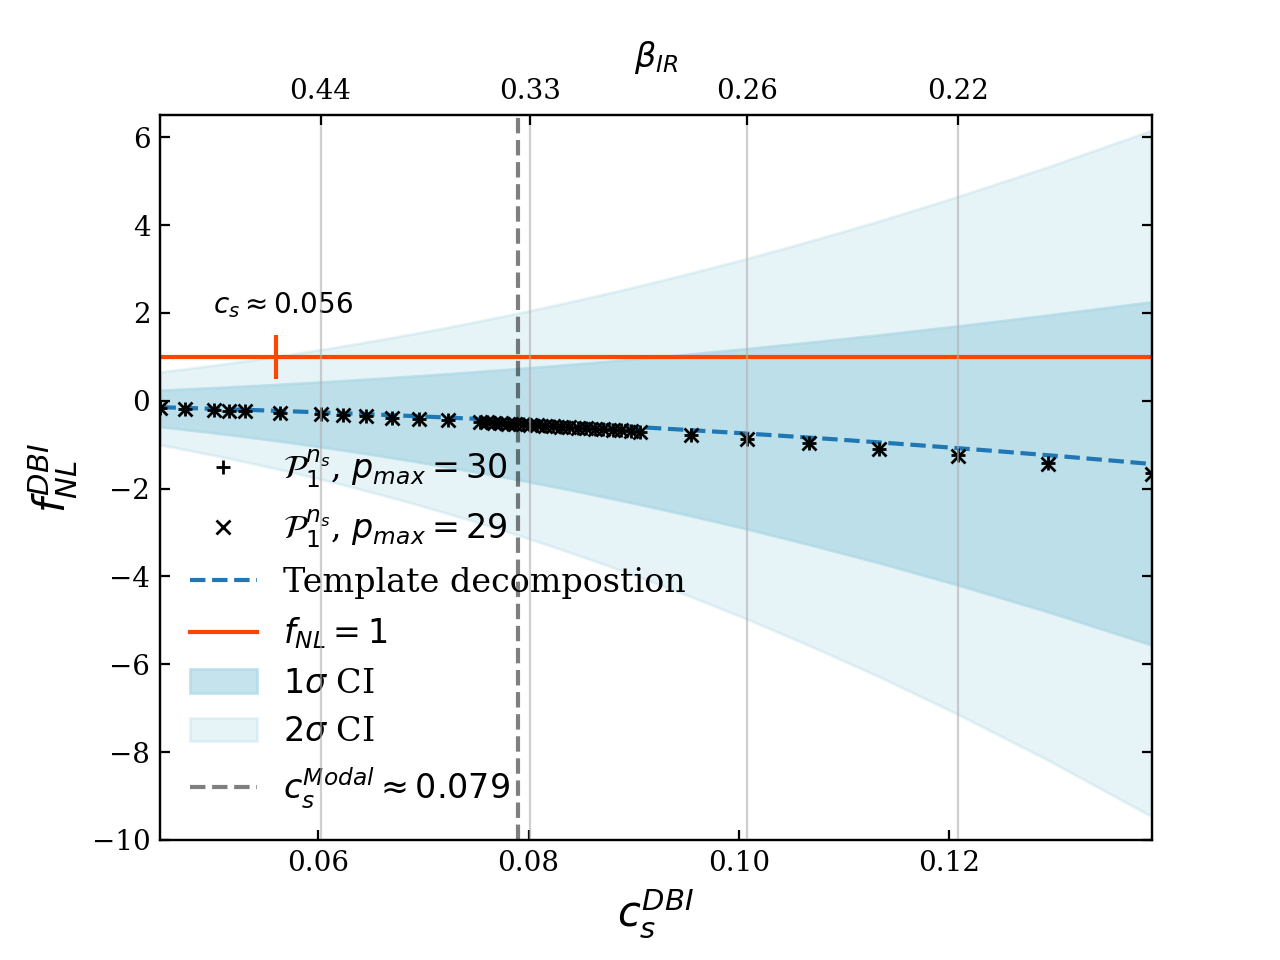
\includegraphics[width=0.9\textwidth]{wuhyun_plots/beta_ir_constraint_busy.png}
        \caption{
            Our constraint on DBI inflation. Here $c_s^{DBI}$ is not an input parameter
            (unlike in the template case), instead it is time dependent, and the plotted
            value is taken from the horizon crossing of the pivot scale. We find that $\beta_{IR}<0.5$
            %0.464
            is outside of our $2\sigma$ confidence interval. This plot was obtained by
            scanning across values of $\beta_{IR}$ and calculating the corresponding primordial bispectra
            using $\primodal$, then projecting those bispectra onto the $\cmb$
            and comparing them to the $\planck$ $\cmb$ temperature data using
            $\cmbbest$. Since the amplitude is fixed by the scenario, we rule out a
            scenario by ruling out $f_{NL}^{DBI}=1$.
            Note that the constraint obtained for $\Pmax=30$ and $\Pmax=29$ is identical,
            so we can be confident that our constraint has converged in $\Pmax$.
            We can see that the $\cmbbest$ result does not agree with the $\modal$ result,
            but as we see in figure~\ref{fig:equil_constraints_comparison},
            the discrepancy is not unexpected. We discuss possible explanations
            \textcolor{red}{in the text}.
        }\label{fig:dbi_sound_speed_scan_beta}
    \end{figure}
    \begin{figure}[htbp!]
        \centering
        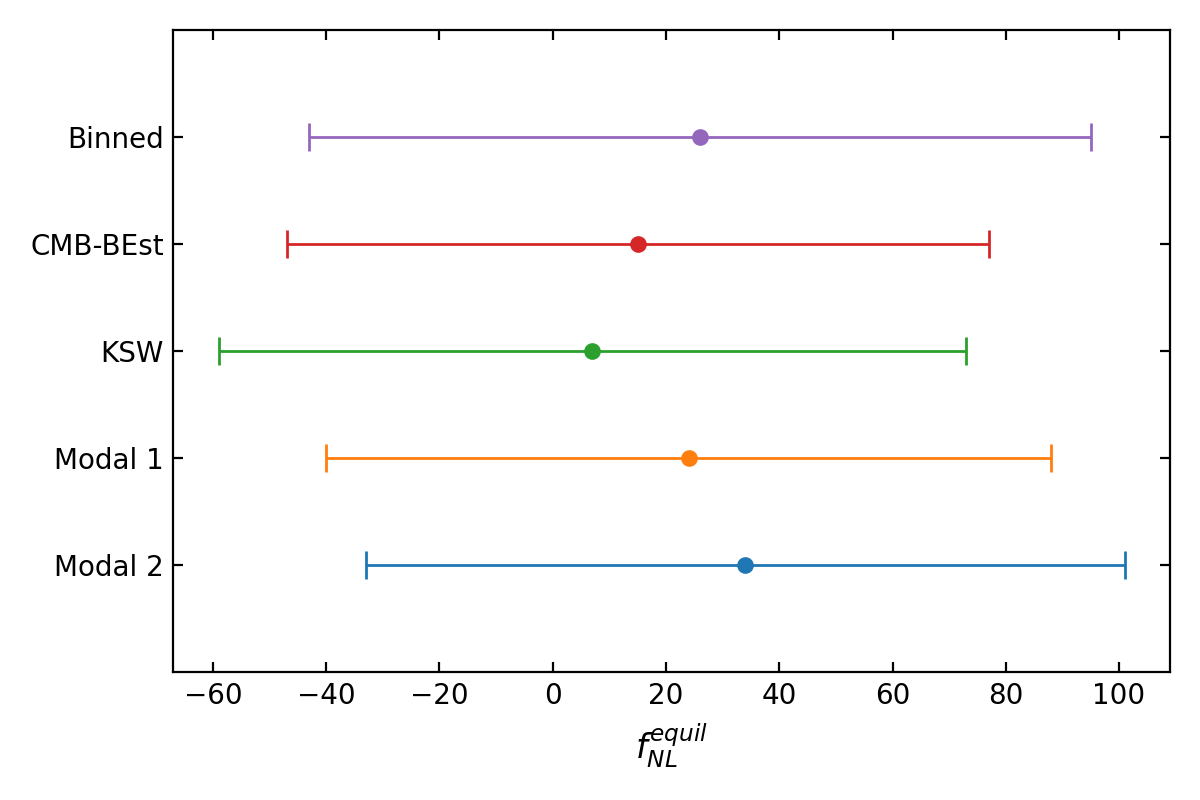
\includegraphics[width=0.9\textwidth]{wuhyun_plots/fnl_equil_planck_scatter.png}
        \caption{
            A comparison of the various estimation methods used in $\planck$
            (as presented in table 5 of~\cite{Planck_NG_2018}).
            We plot the constraints obtained by each method for $\fnlequil$,
            as well as the constraint obtained by $\cmbbest$ (presented in~\cite{Sohn_2021})
            along with their $68\%$ uncertainty margin.
            We see that while the estimators do not agree, there is no discrepancy with any
            significance---in particular, we see that $\cmbbest$ is not an outlier.
        }\label{fig:equil_constraints_comparison}
    \end{figure}

\section{Then, check how the scaling from the real numerical result affects this.}
    Here we will compare template decompositions to Primodal results.
    This will tell us how large the slow-roll corrections are to the
    final CMB result, but not anything about the primordial convergence.
    The main slow-roll corrections are a correction to the amplitude,
    and a deviation from perfect scale-dependence.
%\section{EFT stuff, build off Enrico's recent work.}
%    Words


%%%%%%%%%%%%%%%%%%%%%%%%%%%%%%%%%%%%%%%%%%%%%%%%%%%%%%%%%%%%%%%%%%%%%%%%%%%%%%%%
%% Chapter 5:
%%
\chapter{Conclusions}\label{chapter:conclusion}

\section{Summary}
Through the work detailed in this thesis the inherent separability of the tree level in-in formalism
has been exploited, using expansions in separable basis functions.
Following the modal philosophy of~\cite{FergShell_1,FergShell_2,FergShell_3}, and building on the basic idea of~\cite{Funakoshi},
this method obviates the requirement of considering an approximate separable template,
which was a limitation of previous analyses. Instead,
the goal is to work with the full numerically calculated tree-level inflationary bispectrum of the scenario
being considered. The output is not a grid of points, but a set of coefficients of
the explicitly separable basis expansion.
This preserves the separability and therefore allows us to skip the usual template-approximation step.
We have:
\begin{itemize}
    \item developed practical sets of such basis functions, showing the overall method
to be feasible by testing them on realistic and interesting shapes.
    \item developed efficient and robust methods of applying the in-in formalism
to an inflation scenario, to generate shape coefficients for some given basis.
    \item applied these methods to a particular
inflation scenario, and used the separability of our result to connect to the methods of~\cite{Sohn_2021}.
This allowed us to place a constraint on that scenario, using $\planck$ $\cmb$ data.
\end{itemize}
Through this work we developed this separable approach into a practical and efficient numerical methodology.
%allowing it to be applied to a
%wider and more complicated range of bispectrum phenomenology than previously,
%as we demonstrated in our validation examples.
%This is an important step forward towards observational
%pipelines which can directly confront specific models of inflation using the full bispectrum
%information in a template-free analysis.
These methods and basis sets have been implemented in the $\primodal$ code, which calculates
the shape coefficients for a given inflation scenario, in a given basis.
We have explored and contrasted the advantages of the various basis sets we described, and thoroughly
validated our methods on single-field inflation models with non-trivial phenomenology.
This validation showed that our calculation of these coefficients is fast and accurate to high orders.


The latter part of this bispectrum estimation pipeline
connects the shape coefficient output of $\primodal$ to the $\cmb$.
This part of the pipeline is described and
validated in~\cite{Sohn_2021} and implemented in the $\cmbbest$ code.
In chapter~\ref{chapter:constraints} we tested the integration of the $\primodal$ and $\cmbbest$
parts of the pipeline.
We scanned across a fundamental parameter, $\bir$, of the $\dbi$ model of inflation.
Our goal was to obtain a constraint on this parameter using our
template-free analysis---we found 
$\bir\le0.46$ at $95\%$ confidence using $\planck$ temperature data.
This differed from the equivalent constraint found by the $\modal$ estimator
in the $\planck$ analysis, but the results were sufficiently in agreement that we
can take this as a broad validation of our pipeline.


\section{Discussion}
In this work we recast the calculation of the tree-level primordial bispectrum~\eqref{inin_integral}
into a form that explicitly preserves its separability.
We emphasise again that this work has two main advantages over previous
numerical methods. The more immediate is that by calculating the primordial
bispectrum in terms of an expansion in some basis, the full bispectrum can
be obtained much more efficiently than through repetitive integration
separately for each $k$-configuration. The second (and more important)
advantage is the link to observations.
Unlike previous numerical and semi-analytic methods,
once the shape function is expressed in some basis as in~\eqref{goal},
the integral~\eqref{eq:reduced_cmb} and other computationally intensive steps involved
in estimating a particular bispectrum in the $\cmb$, can be precomputed. Since this
large cost is only paid once per basis, once a basis
which converges well for a broad range of models
has been found, an extremely broad exploration of primordial bispectra becomes immediately feasible in the $\cmb$.
%Making explicit the $k$-dependence in this way also opens the door to vast increases in efficiency in
%connecting to other observables, by precomputation using the basis set, then performing a (relatively) cheap
%scan over inflation parameters.


Our work here goes beyond that of~\cite{Funakoshi} in that our careful methodology
allows us to accurately and efficiently go to much higher orders.
%in particular our methods of starting the time integrals~\eqref{inin_kindep}
%and of including the spatial derivative terms in the calculation.
This allowed us to present this method for feature bispectra for the first time,
with linear oscillations, logarithmic oscillations, and complicated shape dependence.
%demonstrating the efficient exploration of much more general primordial bispectrum phenomenology.
We also identified and addressed the effects
of the non-physical $k$-configurations on convergence within the three-dimensional tetrapyd.
We explored, for the first time, possible basis set choices in the context of those effects.
We showed rapid convergence on a broad range of scenarios,
including cases with oscillatory features with non-trivial shape dependence,
using our augmented basis sets.


The immediate application of this work is the efficient exploration of
bispectrum phenomenology, as our methods can much more quickly
converge to the full shape information than previous numerical methods,
which relied on calculating the shape function point-by-point, for each $k$-configuration separately.
We have implemented these methods for single field scenarios
with a varying sound speed, scenarios which
have a rich feature phenomenology. An important goal, however, will be extending
these methods to the case of multiple-field inflation.
These goals support those laid out in the recent community white paper~\cite{astro2020_png},
by improving predictions of the phenomenology of non-linearities in the very early universe.
%The ability to efficiently compare the phenomenology of these scenarios to observation and thus
%constrain the space of theories is a very worthwhile goal, though the phenomenology is also of interest in its own right.

While the phenomenology is of interest in its own right,
the main advantage of our methods is that it will enable
direct constraints of parameters of inflationary scenarios which do not have
standard bispectrum templates, thus obtaining new constraints on inflationary parameters.
These new constraints will come from exploiting the existing $\planck$ data in
new ways, and from data from future experiments.
Using the basis sets and the separable formulation of the in-in calculation developed in this work,
%it will be possible to reproduce and improve upon the established constraints on inflation models,
it will be possible to obtain constraints using the full shape dependence,
strengthening the connection between the very early universe and the universe we
find ourselves in today.


%%%%%%%%%%%%%%%%%%%%%%%%%%%%%%%%%%%%%%%%%%%%%%%%%%%%%%%%%%%%%%%%%%%%%%%%%%%%%%%%
%% References:
%%
% If you include some work not referenced in the main text (e.g. using \nocite{}), consider changing "References" to "Bibliography".
%

% \renewcommand to change default "Bibliography" to "References"
\renewcommand{\bibname}{References}
\cleardoublepage
\phantomsection
\addcontentsline{toc}{chapter}{References}
\nocite{*}
\bibliographystyle{JHEP}
\bibliography{thesis}



%%%%%%%%%%%%%%%%%%%%%%%%%%%%%%%%%%%%%%%%%%%%%%%%%%%%%%%%%%%%%%%%%%%%%%%%%%%%%%%%
%% Appendix:
%%

\appendix

\chapter{Appendices}
\section{Efficient numerics}
Efficient evaluation and numerical usage of the coefficients (vander, etc).
Numeric choices that aren't specific to mode evolution, etc.
Gauss-Legendre integration, fixed weights.
\section{Tools used}
Numpy, Scipy, Jupyter Notebooks, QUADPTS...?
\section{Transport method for the Modal coeffs}\label{appendix_modal_transport}
Infinite hierarchy of coupled equations.
Choose a basis to make it nice?
Real vs Imag...?
Sounds cool, not worth pursuing.
One could imagine applying the same philosophy to our method.
Certainly, at first sight this seems more natural, that if the core
quantities in our method are the coefficients in some basis expansion,
why not evolve them directly? Why take the apparently circuitous route
of evolving the $\zeta_k(\tau)$, and decomposing them at every timestep?
The answer is that the ``equations of motion'' for the coefficients of the expansion
obtained by substituting the mode expansion of $\zeta_k(\tau)$ into~\eqref{modefneqn}
are coupled in an infinite hierarchy.



%%%%%%%%%%%%%%%%%%%%%%%%%%%%%%%%%%%%%%%%%%%%%%%%%%%%%%%%%%%%%%%%%%%%%%%%%%%%%%%%
%% Index:
%%
\printthesisindex

\end{document}
